
\documentclass[11pt,twoside]{book}
%Versión 4.0
% paquetes-----------------------------------------------------------------------------------------
\usepackage{lipsum} % para pruebas
\usepackage{pdftexcmds} %Para switch case
\usepackage[
paperwidth = 8.5in,
paperheight = 11in,
left = 1.25in,
right = 0.75in,
top = 0.950in,
bottom = 0.925in
]{geometry}
\usepackage{varwidth}
\usepackage{amsmath}
\usepackage{amsfonts}
\usepackage{amssymb}
\usepackage{graphicx}
\usepackage{pdfpages}
\usepackage{setspace} 
\usepackage{xltxtra}
\usepackage{enumitem}
\usepackage{xifthen}
\usepackage{xargs}
\usepackage{booktabs}
\usepackage{multirow}
\usepackage{pdflscape}
\usepackage{rotating}
\usepackage{bigstrut}
\usepackage{longtable}
\usepackage{fancyhdr}
\usepackage{url}
\usepackage{tocloft}
\usepackage[hidelinks, verbose]{hyperref}
\usepackage{colortbl}
\usepackage{multirow}
\usepackage{multicol}
\usepackage{changepage}
\usepackage[skins, breakable, hooks]{tcolorbox}
\usepackage[input-decimal-markers={.}, input-ignore={,}, group-separator={,}]{siunitx}
\usepackage{polyglossia}
\usepackage{tikz}
\usetikzlibrary{calc}
\usetikzlibrary{positioning}
\usepackage{array}
\usepackage{ragged2e} %Sirve para justificar texto
% \usepackage{fontspec} % se carga en xltxtra
% \usepackage{fixltx2e} % fixltx2e is not required with releases after 2015. All fixes are now in the LaTeX kernel.
% FIN-paquetes-------------------------------------------------------------------------------------
\setlength{\columnsep}{1.1cm} % estaba luego de multicol
\strictpagecheck % algo de changepage
\setmainlanguage{spanish} % de polyglossia
% leer pag 4 https://mirrors.ucr.ac.cr/CTAN/macros/latex/required/tools/array.pdf
% nuevos tipos de columnas
\newcolumntype{x}[1]{>{\centering\arraybackslash}p{#1}}
\newcolumntype{g}[1]{>{\raggedleft\arraybackslash}p{#1}}
\newcolumntype{q}[1]{>{\raggedright\arraybackslash}p{#1}}
% Tipo de letra
\usepackage[abspath]{currfile}
\setmainfont[
	Path=\currfileabsdir,
	BoldFont = Fuentes/OpenSans-CondBold.ttf ,
	ItalicFont = Fuentes/OpenSans-CondLightItalic.ttf ,
	BoldItalicFont = Fuentes/OpenSans-CondLightItalic.ttf
]{OpenSans-CondLight.ttf}
\newfontfamily\Bold{Open Sans Condensed Bold}
\newfontfamily\Sans{Open Sans}
\newfontfamily\SansBold{Open Sans Bold}
\newfontfamily\Italic{Open Sans Condensed Light Italic}
\newfontfamily\Logos{Latin Modern Roman}
\newfontfamily\Cinzel{Open Sans}
% diagramas de tikz
\tikzset{
    max width/.style args={#1}{
        execute at begin node={\begin{varwidth}{#1}},
        execute at end node={\end{varwidth}}
    }
}
\usetikzlibrary{shapes.geometric, arrows}
\tikzstyle{arrow} = [thick,->,>=stealth, to path={-| (\tikztotarget)}]
\tikzstyle{iniciofin} = [rectangle, minimum width=2cm, minimum height=0.7cm, text centered, draw=black, fill=blue!30, rounded corners]
\tikzstyle{process} = [rectangle, minimum width=3.5cm, minimum height=2cm, text centered, draw=black, max width=3.5cm]
\tikzstyle{decision} = [diamond, minimum width=3cm, minimum height=1cm, text centered, draw=black]
\tikzstyle{aux} = [fill=white,inner sep=0,outer sep=0]
\tikzstyle{diagrama} = [node distance=4cm, auto,scale=0.7, every node/.style={scale=0.7}]

% Estilo de página en blanco en el índice
\newcommand{\blank}{\addtocontents{toc}{\protect\thispagestyle{empty}}}

%título y fuente
\newcommand{\titulodoc}{Nombre del documento}
\newcommand{\lafuente}{Estadísticas INE}

\newcounter{Cuadro}[chapter]
\renewcommand{\theCuadro}{\thechapter.\arabic{Cuadro}}

\newcommand{\titulocuadro}[1]{\addtocounter{Cuadro}{1}
{\Bold\color{color1}{\normalsize Cuadro \theCuadro $\,-$  #1 }}
}

%%%%%%%%%%% Diseño global del documento
%	\setlength{\headsep}{0pt}
%	\setlength{\footskip}{46pt}
\setlength{\parindent}{1.5em}		%sangría
\setlength{\parskip}{2ex}		%separación entre párrafos  

%Distancias
\newlength{\cuadri} 
\setlength{\cuadri}{0.125in}

%Formato de contenidos
\setlength{\cftbeforetoctitleskip}{0em}
\AtBeginDocument{\addtocontents{toc}{\protect\thispagestyle{empty}}} 

\makeatletter
\renewcommand*\l@subsection{\@dottedtocline{2}{5.2em}{3.2em}}
\makeatother

\renewcommand{\thesection}{\thechapter.\arabic{section}}

\cftsetpnumwidth{2\cuadri}
\cftsetrmarg{8\cuadri}
\renewcommand{\cftsecnumwidth}{2.5\cuadri}
\renewcommand{\cftchapnumwidth}{2\cuadri}
\renewcommand{\cftsecindent}{2\cuadri}

%Colores base del documento
\definecolor{color1}{rgb}{0,0,0} % -Negro
%\definecolor{color2}{rgb}{0.56,0.36,0.65} %Debe ir en porcentaje de rgb (i.e. decimal) - morado rosadón
\definecolor{color2}{rgb}{0.45,0.44,0.78} % - Lila
%\definecolor{color2}{rgb}{0.09,0.47,0.27} % - Verde feminista
\definecolor{color3}{rgb}{0.2,0.2,0.5} %Debe ir en porcentaje de rgb (i.e. decimal) - Morado oscuro

%Para que las páginas en blanco no estén numeradas
\let\origdoublepage\cleardoublepage
\newcommand{\clearemptydoublepage}{
\clearpage
{\pagestyle{empty}\origdoublepage}
}
\let\cleardoublepage\clearemptydoublepage

%%%%%%%% Llamadas y notas al pie
\makeatletter
\newcommand{\markerspace}{\@ifnextchar.
{$\!$}{\@ifnextchar,
    {$\!$}{\@ifnextchar;
        {$\!$}{\@ifnextchar:
            {$\!$}{$\ $}
        }
    }
}}
\makeatother

\newcounter{numllamada}
\newcounter{numtextollamada}
\setcounter{numllamada}{0}
\setcounter{numtextollamada}{0}

\newcommand{\llamada}[1][\thenumllamada]{
	\stepcounter{numllamada}
	\begingroup
	\setcounter{mpfootnote}{#1}
	\renewcommand\thefootnote\thempfootnote$\hspace{0.2ex}$\footnotemark
	\endgroup
	\markerspace
}

\newcommand{\notita}[2][\thenumtextollamada]{
\stepcounter{numtextollamada}
\stepcounter{numllamada}
$\hspace{0.2ex}$
\footnote[#1]{#2}
}

\newcommand{\textollamada}[2][\thenumtextollamada]{
\ifthenelse{\equal{#1}{*}}
{
\begingroup
\renewcommand\thefootnote\thempfootnote\footnotetext[0]{#2\\[-1.7ex]}
\endgroup
}{
\stepcounter{numtextollamada}
\begingroup
\renewcommand\thefootnote\thempfootnote\footnotetext[#1]{#2}
\endgroup
}}

%redefinición de footnote
\newlength{\footnoterulewidth}
\setlength{\footnoterulewidth}{2.5cm}
\newlength{\footnoteruleheight}
\setlength{\footnoteruleheight}{.4pt} 
\makeatletter
\renewcommand{\footnoterule}{
	\kern -3pt
	\color{color2}
	\hrule width 
	\footnoterulewidth height 
	\footnoteruleheight
	\kern
	\dimexpr 3pt - \footnoteruleheight \relax
} 
\makeatother

\makeatletter
\renewcommand\@makefntext[1]{
	\noindent
	\makebox[1em][r]{\scriptsize\@makefnmark}
	\scriptsize#1
}
\makeatother

%%%%%%%%%%% tablas
\LTcapwidth=1.234\textwidth
\setlength{\arrayrulewidth}{0.8pt}
\arrayrulecolor{color2}

% Definición del comando cajita

\newtcolorbox{cajita-arriba}{
	width = 52\cuadri,
	height = 35\cuadri,
	enlarge left by = 0pt,
	enlarge top by = 1\cuadri,
	enlarge bottom by = 2\cuadri,
	nobeforeafter,
	opacityback=0, % Pone fondo transparente
	opacityframe=0, % Pone fondo transparente
	colframe=black, % Pone fondo transparente
%	colframe = white, % obsoleto, se dejó para referencia
%	colback = white, % obsoleto, se dejó para referencia
	left = -3pt,
	right = 0pt,
	bottom = 0pt,
	top = -3pt,
	arc = 0pt,
	boxrule = 0pt
}

\newtcolorbox{cajita-abajo}{
	width = 52\cuadri,
	height = 35\cuadri,
	enlarge top by = 0pt,
	enlarge left by = 0pt,
	enlarge bottom by = -2\cuadri,
	nobeforeafter,
	opacityback=0, % Pone fondo transparente
	opacityframe=0, % Pone fondo transparente
	colframe=black, % Pone fondo transparente
%	colframe = white, % obsoleto, se dejó para referencia
%	colback = white, % obsoleto, se dejó para referencia
	left = -3pt,
	right = 0pt,
	bottom = 0pt,
	top = -3pt,
	arc = 0pt,
	boxrule = 0pt
}

\newtcolorbox{cajota-unica}{
	width = 52\cuadri,
	height = 72\cuadri,
	enlarge left by = 0pt,
	enlarge top by  = 1\cuadri,
	enlarge bottom by = -2\cuadri,
	nobeforeafter,
	opacityback=0, % Pone fondo transparente
	opacityframe=0, % Pone fondo transparente
	colframe=black, % Pone fondo transparente
%	colframe = white, % obsoleto, se dejó para referencia
%	colback = white, % obsoleto, se dejó para referencia
	left = -3pt,
	right = 0pt,
	bottom =  0pt,
	top = -3pt,
	arc = 0pt,
	boxrule = 0pt
}

\newtcolorbox{descripcion-cajita}{
	width = 18\cuadri,
	height = 30.8\cuadri,
	nobeforeafter,
	opacityback=0, % Pone fondo transparente
	opacityframe=0, % Pone fondo transparente
	colframe=black, % Pone fondo transparente
	%colframe = white, % obsoleto, se dejó para referencia 
	%colback = white, % obsoleto, se dejó para referencia 
	left = -3pt,
	right = -3pt,
	bottom = -3pt,
	top = -8pt,
	arc = 0pt,
	boxrule = 0pt,
	enlarge bottom by = -29.78\cuadri
}

\newtcolorbox{grafica-cajita}{
	width = 32\cuadri,
	height = 30.8\cuadri,
	nobeforeafter,
	opacityback=0, % Pone fondo transparente
	opacityframe=0, % Pone fondo transparente
	colframe=black, % Pone fondo transparente
%	colframe = white, % obsoleto, se dejó para referencia
%	colback = white, % obsoleto, se dejó para referencia
	left = -3pt,
	right = -3pt,
	bottom = -3pt,
	top = -2pt,
	arc = 0pt,
	boxrule = 0pt,
	enlarge bottom by = -29.78\cuadri
}
% Cajas para fondos de capítulo y encabezado
\newtcolorbox{fondo-capitulo}{
	width = 8.5in,
	height = 11in,
	skin = enhancedmiddle, 
	nobeforeafter,
	watermark graphics = Plantilla/Capitulo_CEEG_2022.pdf,
	watermark opacity = 1.0,
	watermark overzoom = 1.0,
	enlarge left by=-1.475in,
	enlarge top by = -0.95in,
	enlarge bottom by = -20\cuadri,
	boxrule = 0pt,
	colframe = white,
	left = -3pt,
	bottom = -1pt,
	top = 8\cuadri,
	right = -3pt,
	arc = 0pt
}

% Cajas para agregar ODS



\newcommand{\cajitaODS}[1]{%
	\ifthenelse{ \equal{#1}{1} }{%
			\begin{tcolorbox}[
			width = 1.5cm,
	height = 1.5cm,
	skin = enhancedmiddle, 
	nobeforeafter,
	watermark graphics = Plantilla/ODS/ods1.pdf,
	watermark opacity = 1.0,
	watermark overzoom = 1.0,
	enlarge top by = 0.01in,
	enlarge bottom by = -1.5cm,
	boxrule = 0pt,
	colframe = white,
	colback = white,
	left = -3pt,
	bottom = -5in,
	top = -10\cuadri,
	right = -3pt,
	arc = 0pt]
\end{tcolorbox}	
	}%
	{}%
	\ifthenelse{\equal{#1}{2}}{%
			\begin{tcolorbox}[
			width = 1.5cm,
			height = 1.5cm,
			skin = enhancedmiddle, 
			nobeforeafter,
			watermark graphics = Plantilla/ODS/ods2.pdf,
			watermark opacity = 1.0,
			watermark overzoom = 1.0,
			enlarge top by = 0.01in,
			enlarge bottom by = -1.5cm,
			boxrule = 0pt,
			colframe = white,
			colback = white,
			left = -3pt,
			bottom = -5in,
			top = -10\cuadri,
			right = -3pt,
			arc = 0pt]
		\end{tcolorbox}	
	}%
	{}
		\ifthenelse{\equal{#1}{3}}{%
			\begin{tcolorbox}[
			width = 1.5cm,
	height = 1.5cm,
	skin = enhancedmiddle, 
	nobeforeafter,
	watermark graphics = Plantilla/ODS/ods3.pdf,
	watermark opacity = 1.0,
	watermark overzoom = 1.0,
	enlarge top by = 0.01in,
	enlarge bottom by = -1.5cm,
	boxrule = 0pt,
	colframe = white,
	colback = white,
	left = -3pt,
	bottom = -5in,
	top = -10\cuadri,
	right = -3pt,
	arc = 0pt]
\end{tcolorbox}	
	}%
	{}
		\ifthenelse{\equal{#1}{4}}{%
			\begin{tcolorbox}[
	width = 1.5cm,
	height = 1.5cm,
	skin = enhancedmiddle, 
	nobeforeafter,
	watermark graphics = Plantilla/ODS/ods4.pdf,
	watermark opacity = 1.0,
	watermark overzoom = 1.0,
	enlarge top by = 0.01in,
	enlarge bottom by = -1.5cm,
	boxrule = 0pt,
	colframe = white,
	colback = white,
	left = -3pt,
	bottom = -5in,
	top = -10\cuadri,
	right = -3pt,
	arc = 0pt]
\end{tcolorbox}	
	}%
	{}
		\ifthenelse{\equal{#1}{5}}{%
			\begin{tcolorbox}[
	width = 1.5cm,
	height = 1.5cm,
	skin = enhancedmiddle, 
	nobeforeafter,
	watermark graphics = Plantilla/ODS/ods5.pdf,
	watermark opacity = 1.0,
	watermark overzoom = 1.0,
	enlarge top by = 0.01in,
	enlarge bottom by = -1.5cm,
	boxrule = 0pt,
	colframe = white,
	colback = white,
	left = -3pt,
	bottom = -5in,
	top = -10\cuadri,
	right = -3pt,
	arc = 0pt]
\end{tcolorbox}	
	}%
	{}
		\ifthenelse{\equal{#1}{6}}{%
			\begin{tcolorbox}[
	width = 1.5cm,
	height = 1.5cm,
	skin = enhancedmiddle, 
	nobeforeafter,
	watermark graphics = Plantilla/ODS/ods6.pdf,
	watermark opacity = 1.0,
	watermark overzoom = 1.0,
	enlarge top by = 0.01in,
	enlarge bottom by = -1.5cm,
	boxrule = 0pt,
	colframe = white,
	colback = white,
	left = -3pt,
	bottom = -5in,
	top = -10\cuadri,
	right = -3pt,
	arc = 0pt]
\end{tcolorbox}	
	}%
	{}
		\ifthenelse{\equal{#1}{7}}{%
			\begin{tcolorbox}[
	width = 1.5cm,
	height = 1.5cm,
	skin = enhancedmiddle, 
	nobeforeafter,
	watermark graphics = Plantilla/ODS/ods7.pdf,
	watermark opacity = 1.0,
	watermark overzoom = 1.0,
	enlarge top by = 0.01in,
	enlarge bottom by = -1.5cm,
	boxrule = 0pt,
	colframe = white,
	colback = white,
	left = -3pt,
	bottom = -5in,
	top = -10\cuadri,
	right = -3pt,
	arc = 0pt]
\end{tcolorbox}	
	}%
	{}
		\ifthenelse{\equal{#1}{8}}{%
			\begin{tcolorbox}[
	width = 1.5cm,
	height = 1.5cm,
	skin = enhancedmiddle, 
	nobeforeafter,
	watermark graphics = Plantilla/ODS/ods8.pdf,
	watermark opacity = 1.0,
	watermark overzoom = 1.0,
	enlarge top by = 0.01in,
	enlarge bottom by = -1.5cm,
	boxrule = 0pt,
	colframe = white,
	colback = white,
	left = -3pt,
	bottom = -5in,
	top = -10\cuadri,
	right = -3pt,
	arc = 0pt]
\end{tcolorbox}	
	}%
	{}
	
			\ifthenelse{\equal{#1}{9}}{%
		\begin{tcolorbox}[
			width = 1.5cm,
			height = 1.5cm,
			skin = enhancedmiddle, 
			nobeforeafter,
			watermark graphics = Plantilla/ODS/ods9.pdf,
			watermark opacity = 1.0,
			watermark overzoom = 1.0,
			enlarge top by = 0.01in,
			enlarge bottom by = -1.5cm,
			boxrule = 0pt,
			colframe = white,
			colback = white,
			left = -3pt,
			bottom = -5in,
			top = -10\cuadri,
			right = -3pt,
			arc = 0pt]
		\end{tcolorbox}	
	}%
	{}
	
			\ifthenelse{\equal{#1}{10}}{%
		\begin{tcolorbox}[
			width = 1.5cm,
			height = 1.5cm,
			skin = enhancedmiddle, 
			nobeforeafter,
			watermark graphics = Plantilla/ODS/ods10.pdf,
			watermark opacity = 1.0,
			watermark overzoom = 1.0,
			enlarge top by = 0.01in,
			enlarge bottom by = -1.5cm,
			boxrule = 0pt,
			colframe = white,
			colback = white,
			left = -3pt,
			bottom = -5in,
			top = -10\cuadri,
			right = -3pt,
			arc = 0pt]
		\end{tcolorbox}	
	}%
	{}
	
			\ifthenelse{\equal{#1}{11}}{%
		\begin{tcolorbox}[
			width = 1.5cm,
			height = 1.5cm,
			skin = enhancedmiddle, 
			nobeforeafter,
			watermark graphics = Plantilla/ODS/ods11.pdf,
			watermark opacity = 1.0,
			watermark overzoom = 1.0,
			enlarge top by = 0.01in,
			enlarge bottom by = -1.5cm,
			boxrule = 0pt,
			colframe = white,
			colback = white,
			left = -3pt,
			bottom = -5in,
			top = -10\cuadri,
			right = -3pt,
			arc = 0pt]
		\end{tcolorbox}	
	}%
	{}
	
			\ifthenelse{\equal{#1}{12}}{%
		\begin{tcolorbox}[
			width = 1.5cm,
			height = 1.5cm,
			skin = enhancedmiddle, 
			nobeforeafter,
			watermark graphics = Plantilla/ODS/ods12.pdf,
			watermark opacity = 1.0,
			watermark overzoom = 1.0,
			enlarge top by = 0.01in,
			enlarge bottom by = -1.5cm,
			boxrule = 0pt,
			colframe = white,
			colback = white,
			left = -3pt,
			bottom = -5in,
			top = -10\cuadri,
			right = -3pt,
			arc = 0pt]
		\end{tcolorbox}	
	}%
	{}
	
			\ifthenelse{\equal{#1}{13}}{%
		\begin{tcolorbox}[
			width = 1.5cm,
			height = 1.5cm,
			skin = enhancedmiddle, 
			nobeforeafter,
			watermark graphics = Plantilla/ODS/ods13.pdf,
			watermark opacity = 1.0,
			watermark overzoom = 1.0,
			enlarge top by = 0.01in,
			enlarge bottom by = -1.5cm,
			boxrule = 0pt,
			colframe = white,
			colback = white,
			left = -3pt,
			bottom = -5in,
			top = -10\cuadri,
			right = -3pt,
			arc = 0pt]
		\end{tcolorbox}	
	}%
	{}
	
			\ifthenelse{\equal{#1}{14}}{%
		\begin{tcolorbox}[
			width = 1.5cm,
			height = 1.5cm,
			skin = enhancedmiddle, 
			nobeforeafter,
			watermark graphics = Plantilla/ODS/ods14.pdf,
			watermark opacity = 1.0,
			watermark overzoom = 1.0,
			enlarge top by = 0.01in,
			enlarge bottom by = -1.5cm,
			boxrule = 0pt,
			colframe = white,
			colback = white,
			left = -3pt,
			bottom = -5in,
			top = -10\cuadri,
			right = -3pt,
			arc = 0pt]
		\end{tcolorbox}	
	}%
	{}
	
			\ifthenelse{\equal{#1}{15}}{%
		\begin{tcolorbox}[
			width = 1.5cm,
			height = 1.5cm,
			skin = enhancedmiddle, 
			nobeforeafter,
			watermark graphics = Plantilla/ODS/ods15.pdf,
			watermark opacity = 1.0,
			watermark overzoom = 1.0,
			enlarge top by = 0.01in,
			enlarge bottom by = -1.5cm,
			boxrule = 0pt,
			colframe = white,
			colback = white,
			left = -3pt,
			bottom = -5in,
			top = -10\cuadri,
			right = -3pt,
			arc = 0pt]
		\end{tcolorbox}	
	}%
	{}
	
			\ifthenelse{\equal{#1}{16}}{%
		\begin{tcolorbox}[
			width = 1.5cm,
			height = 1.5cm,
			skin = enhancedmiddle, 
			nobeforeafter,
			watermark graphics = Plantilla/ODS/ods16.pdf,
			watermark opacity = 1.0,
			watermark overzoom = 1.0,
			enlarge top by = 0.01in,
			enlarge bottom by = -1.5cm,
			boxrule = 0pt,
			colframe = white,
			colback = white,
			left = -3pt,
			bottom = -5in,
			top = -10\cuadri,
			right = -3pt,
			arc = 0pt]
		\end{tcolorbox}	
	}%
	{}
	
			\ifthenelse{\equal{#1}{17}}{%
		\begin{tcolorbox}[
			width = 1.5cm,
			height = 1.5cm,
			skin = enhancedmiddle, 
			nobeforeafter,
			watermark graphics = Plantilla/ODS/ods17.pdf,
			watermark opacity = 1.0,
			watermark overzoom = 1.0,
			enlarge top by = 0.01in,
			enlarge bottom by = -1.5cm,
			boxrule = 0pt,
			colframe = white,
			colback = white,
			left = -3pt,
			bottom = -5in,
			top = -10\cuadri,
			right = -3pt,
			arc = 0pt]
		\end{tcolorbox}	
	}%
	{}
	
}

\newcommand{\cajitaODSArriba}[1]{%
				\ifthenelse{\equal{#1}{1}}{%
				\begin{tcolorbox}[
			width = 1.5cm,
			height = 1.5cm,
			skin = enhancedmiddle, 
			nobeforeafter,
			watermark graphics = Plantilla/ODS/ods1.pdf,
			watermark opacity = 1.0,
			watermark overzoom = 1.0,
			enlarge top by = -5mm,
			enlarge bottom by = -1cm,
			boxrule = 0pt,
			colframe = white,
			colback = white,
			arc = 0pt]
		\end{tcolorbox}	
	}%
	{}
	
					\ifthenelse{\equal{#1}{2}}{%
		\begin{tcolorbox}[
			width = 1.5cm,
			height = 1.5cm,
			skin = enhancedmiddle, 
			nobeforeafter,
			watermark graphics = Plantilla/ODS/ods2.pdf,
			watermark opacity = 1.0,
			watermark overzoom = 1.0,
			enlarge top by = -5mm,
			enlarge bottom by = -1cm,
			boxrule = 0pt,
			colframe = white,
			colback = white,
			arc = 0pt]
		\end{tcolorbox}	
	}%
	{}
					\ifthenelse{\equal{#1}{3}}{%
		\begin{tcolorbox}[
			width = 1.5cm,
			height = 1.5cm,
			skin = enhancedmiddle, 
			nobeforeafter,
			watermark graphics = Plantilla/ODS/ods3.pdf,
			watermark opacity = 1.0,
			watermark overzoom = 1.0,
			enlarge top by = -5mm,
			enlarge bottom by = -1cm,
			boxrule = 0pt,
			colframe = white,
			colback = white,
			arc = 0pt]
		\end{tcolorbox}	
	}%
	{}
	
					\ifthenelse{\equal{#1}{4}}{%
		\begin{tcolorbox}[
			width = 1.5cm,
			height = 1.5cm,
			skin = enhancedmiddle, 
			nobeforeafter,
			watermark graphics = Plantilla/ODS/ods4.pdf,
			watermark opacity = 1.0,
			watermark overzoom = 1.0,
			enlarge top by = -5mm,
			enlarge bottom by = -1cm,
			boxrule = 0pt,
			colframe = white,
			colback = white,
			arc = 0pt]
		\end{tcolorbox}	
	}%
	{}
	
					\ifthenelse{\equal{#1}{5}}{%
		\begin{tcolorbox}[
			width = 1.5cm,
			height = 1.5cm,
			skin = enhancedmiddle, 
			nobeforeafter,
			watermark graphics = Plantilla/ODS/ods5.pdf,
			watermark opacity = 1.0,
			watermark overzoom = 1.0,
			enlarge top by = -5mm,
			enlarge bottom by = -1cm,
			boxrule = 0pt,
			colframe = white,
			colback = white,
			arc = 0pt]
		\end{tcolorbox}	
	}%
	{}
	
					\ifthenelse{\equal{#1}{6}}{%
		\begin{tcolorbox}[
			width = 1.5cm,
			height = 1.5cm,
			skin = enhancedmiddle, 
			nobeforeafter,
			watermark graphics = Plantilla/ODS/ods6.pdf,
			watermark opacity = 1.0,
			watermark overzoom = 1.0,
			enlarge top by = -5mm,
			enlarge bottom by = -1cm,
			boxrule = 0pt,
			colframe = white,
			colback = white,
			arc = 0pt]
		\end{tcolorbox}	
	}%
	{}
	
					\ifthenelse{\equal{#1}{7}}{%
		\begin{tcolorbox}[
			width = 1.5cm,
			height = 1.5cm,
			skin = enhancedmiddle, 
			nobeforeafter,
			watermark graphics = Plantilla/ODS/ods7.pdf,
			watermark opacity = 1.0,
			watermark overzoom = 1.0,
			enlarge top by = -5mm,
			enlarge bottom by = -1cm,
			boxrule = 0pt,
			colframe = white,
			colback = white,
			arc = 0pt]
		\end{tcolorbox}	
	}%
	{}
	
					\ifthenelse{\equal{#1}{8}}{%
		\begin{tcolorbox}[
			width = 1.5cm,
			height = 1.5cm,
			skin = enhancedmiddle, 
			nobeforeafter,
			watermark graphics = Plantilla/ODS/ods8.pdf,
			watermark opacity = 1.0,
			watermark overzoom = 1.0,
			enlarge top by = -5mm,
			enlarge bottom by = -1cm,
			boxrule = 0pt,
			colframe = white,
			colback = white,
			arc = 0pt]
		\end{tcolorbox}	
	}%
	{}
	
					\ifthenelse{\equal{#1}{9}}{%
		\begin{tcolorbox}[
			width = 1.5cm,
			height = 1.5cm,
			skin = enhancedmiddle, 
			nobeforeafter,
			watermark graphics = Plantilla/ODS/ods9.pdf,
			watermark opacity = 1.0,
			watermark overzoom = 1.0,
			enlarge top by = -5mm,
			enlarge bottom by = -1cm,
			boxrule = 0pt,
			colframe = white,
			colback = white,
			arc = 0pt]
		\end{tcolorbox}	
	}%
	{}
	
					\ifthenelse{\equal{#1}{10}}{%
		\begin{tcolorbox}[
			width = 1.5cm,
			height = 1.5cm,
			skin = enhancedmiddle, 
			nobeforeafter,
			watermark graphics = Plantilla/ODS/ods10.pdf,
			watermark opacity = 1.0,
			watermark overzoom = 1.0,
			enlarge top by = -5mm,
			enlarge bottom by = -1cm,
			boxrule = 0pt,
			colframe = white,
			colback = white,
			arc = 0pt]
		\end{tcolorbox}	
	}%
	{}
	
					\ifthenelse{\equal{#1}{11}}{%
		\begin{tcolorbox}[
			width = 1.5cm,
			height = 1.5cm,
			skin = enhancedmiddle, 
			nobeforeafter,
			watermark graphics = Plantilla/ODS/ods11.pdf,
			watermark opacity = 1.0,
			watermark overzoom = 1.0,
			enlarge top by = -5mm,
			enlarge bottom by = -1cm,
			boxrule = 0pt,
			colframe = white,
			colback = white,
			arc = 0pt]
		\end{tcolorbox}	
	}%
	{}
	
					\ifthenelse{\equal{#1}{12}}{%
		\begin{tcolorbox}[
			width = 1.5cm,
			height = 1.5cm,
			skin = enhancedmiddle, 
			nobeforeafter,
			watermark graphics = Plantilla/ODS/ods12.pdf,
			watermark opacity = 1.0,
			watermark overzoom = 1.0,
			enlarge top by = -5mm,
			enlarge bottom by = -1cm,
			boxrule = 0pt,
			colframe = white,
			colback = white,
			arc = 0pt]
		\end{tcolorbox}	
	}%
	{}
	
					\ifthenelse{\equal{#1}{13}}{%
		\begin{tcolorbox}[
			width = 1.5cm,
			height = 1.5cm,
			skin = enhancedmiddle, 
			nobeforeafter,
			watermark graphics = Plantilla/ODS/ods13.pdf,
			watermark opacity = 1.0,
			watermark overzoom = 1.0,
			enlarge top by = -5mm,
			enlarge bottom by = -1cm,
			boxrule = 0pt,
			colframe = white,
			colback = white,
			arc = 0pt]
		\end{tcolorbox}	
	}%
	{}
	
					\ifthenelse{\equal{#1}{14}}{%
		\begin{tcolorbox}[
			width = 1.5cm,
			height = 1.5cm,
			skin = enhancedmiddle, 
			nobeforeafter,
			watermark graphics = Plantilla/ODS/ods14.pdf,
			watermark opacity = 1.0,
			watermark overzoom = 1.0,
			enlarge top by = -5mm,
			enlarge bottom by = -1cm,
			boxrule = 0pt,
			colframe = white,
			colback = white,
			arc = 0pt]
		\end{tcolorbox}	
	}%
	{}
	
					\ifthenelse{\equal{#1}{15}}{%
		\begin{tcolorbox}[
			width = 1.5cm,
			height = 1.5cm,
			skin = enhancedmiddle, 
			nobeforeafter,
			watermark graphics = Plantilla/ODS/ods15.pdf,
			watermark opacity = 1.0,
			watermark overzoom = 1.0,
			enlarge top by = -5mm,
			enlarge bottom by = -1cm,
			boxrule = 0pt,
			colframe = white,
			colback = white,
			arc = 0pt]
		\end{tcolorbox}	
	}%
	{}
	
					\ifthenelse{\equal{#1}{16}}{%
		\begin{tcolorbox}[
			width = 1.5cm,
			height = 1.5cm,
			skin = enhancedmiddle, 
			nobeforeafter,
			watermark graphics = Plantilla/ODS/ods16.pdf,
			watermark opacity = 1.0,
			watermark overzoom = 1.0,
			enlarge top by = -5mm,
			enlarge bottom by = -1cm,
			boxrule = 0pt,
			colframe = white,
			colback = white,
			arc = 0pt]
		\end{tcolorbox}	
	}%
	{}
	
					\ifthenelse{\equal{#1}{17}}{%
		\begin{tcolorbox}[
			width = 1.5cm,
			height = 1.5cm,
			skin = enhancedmiddle, 
			nobeforeafter,
			watermark graphics = Plantilla/ODS/ods17.pdf,
			watermark opacity = 1.0,
			watermark overzoom = 1.0,
			enlarge top by = -5mm,
			enlarge bottom by = -1cm,
			boxrule = 0pt,
			colframe = white,
			colback = white,
			arc = 0pt]
		\end{tcolorbox}	
	}%
	{}


}


\newtcolorbox{parte-toc}{
	width = 52\cuadri,
	enlarge left by = 0pt,
	enlarge top by = 0\cuadri,
	enlarge bottom by = 0\cuadri,
	nobeforeafter,
	colframe = color1!90!black,
	colback = white,
	left = 3pt,
	right = 0pt,
	bottom = 0pt,
	top = 0pt,
	arc = 0pt,
	boxrule = 0pt,
	leftrule = 4pt
}

\newtcolorbox{fondo-parte}{
	width=8.5in,
	height=11in,
	skin=enhancedmiddle,
	nobeforeafter,
	watermark graphics=Plantilla/parte.pdf,
	watermark opacity=1.0,
	watermark overzoom=1.0,
	enlarge left by=-1.455in,
	enlarge top by=-0.95in, 
	enlarge bottom by=-20\cuadri,
	boxrule=0pt,
	colframe=white,
	left=-3pt,
	bottom=-1pt,
	top=8\cuadri,
	right=-3pt,
	arc=0pt
}

\newtcolorbox{fondo-capitulo-no-descripcion}{
	width=8.5in,
	height=11in,
	skin=enhancedmiddle,
	nobeforeafter,
	watermark graphics=Plantilla/Apendice_CEEG_2022.pdf,
	watermark opacity=1.0,
	watermark overzoom=1.0,
	enlarge left by=-1.475in,
	enlarge top by=-0.95in,
	enlarge bottom by=-20\cuadri,
	boxrule=0pt,
	colframe=white,
	left=-3pt,
	bottom=-1pt,
	top=8\cuadri,
	right=-3pt,
	arc=0pt
}

\newtcolorbox{numcapitulo}{
	height=1.2in,
	width=1.12in,
	enlarge top by= -1.3in,
	enlarge bottom by=-0.47in,
	boxrule=3pt,arc=3pt,
	colframe=white,
	colback=white,
	right=2pt,
	left=3pt,
	top=14pt,
	bottom=2pt
}

\newtcolorbox{encabezadoimpar}{
	width=8.5in,
	height=11.01in,
	skin=enhancedmiddle,
	nobeforeafter,
	watermark graphics=Plantilla/Cintillo_Derecha_CEEG_2022.pdf,
%	watermark opacity=1.0,
	watermark overzoom=1.0,
	enlarge left by=-1.25in,
	enlarge top by=-0.51in,
	enlarge bottom by=3\cuadri,
	boxrule=0pt, colframe=white,
	left=0.71in,
	bottom=-1pt,
	top=2.5\cuadri,
	right=0.71in,
	arc=0pt
}

\newtcolorbox{encabezadopar}{
	width=8.5in,
	height=11.01in,
	skin=enhancedmiddle,
	nobeforeafter,
	watermark graphics=Plantilla/Cintillo_Izquierda_CEEG_2022.pdf,
	watermark opacity=1.0,
	watermark overzoom=1.0,
	enlarge left by=-0.75in,
	enlarge top by=-0.51in,
	enlarge bottom by=3\cuadri,
	boxrule=0pt,
	colframe=white,
	left=0.71in,
	bottom=-1pt,
	top=2.5\cuadri,
	right=0.71in,
	arc=0pt
}

\newtcbox{numpag}{
	colback=color1,
	colframe=color1,
	arc=0pt,
	top=3pt,
	bottom=2pt,
	left=3pt,
	right=3pt,
	nobeforeafter,
	enlarge top by=-0.125in
}

%%%%%%%%%%% Encabezado y pie de página
\fancypagestyle{estandar}{
	\fancyhf{}
	\renewcommand{\headrulewidth}{0pt}
	\fancyhead[CO]{
		\begin{encabezadoimpar}
		\end{encabezadoimpar}
	}
	\fancyfoot[RO]{
		\color{color3}{\capituloencabezado \ \ }
		\color{color3}
		\raisebox{0.5mm}{$\mid$}
		\color{color3}
		\textbf{ \ \ \ \thepage}
	}
	\fancyhead[CE]{
		\begin{encabezadopar}
		\end{encabezadopar}
	}
	\fancyhead[CO]{
		\begin{encabezadoimpar}
		\end{encabezadoimpar}
	}
	\fancyfoot[LE]{
		\color{color3}
		\textbf{\thepage \ \ \ }
		\color{black}
		\raisebox{0.5mm}{$\mid$}
		\color{color3}{ \ \  \titulodoc}
	}
}

\fancypagestyle{soloarriba}{
	\fancyhf{}
	\renewcommand{\headrulewidth}{0pt}
	\fancyhead[CO]{
		\begin{encabezadoimpar}
		\end{encabezadoimpar}
	}
	\fancyfoot[RO]{}
	\fancyhead[CE]{
		\begin{encabezadopar}
		\end{encabezadopar}
	}
	\fancyfoot[LE]{}
}

\pagestyle{estandar}

%%%%%%%%%%% Macros de cajitas
%  El comando se escribe así: \cajita[Sección en índice]{Sección en cuerpo}{Descripción}{Título gráfica}{Desagregación}{Gráfica con \includegraphics o tikz}{Fuente}
\newcounter{updown}
\setcounter{updown}{0}

\newcommand{\cajitaalternante}[1]{
\ifthenelse{\equal{\theupdown}{0}}{
	\noindent
	\begin{cajita-arriba}
		\phantomsection
		\stepcounter{section} #1
	\end{cajita-arriba}
	\setcounter{updown}{1}
	}{
	\noindent
	\begin{cajita-abajo}
		\phantomsection
		\stepcounter{section} #1
	\end{cajita-abajo}
	\setcounter{updown}{0}
	}
}

\newcommand{\titulizador}[1]{
	\begin{tabular}{@{}p{3.5\cuadri}p{3pt}@{}p{46.0\cuadri}}
		& &\\[-1\cuadri]
		\textbf{\color{color3}\huge \thesection}$\ $ & & \textbf{\color{color3}\huge #1}\\[-1\cuadri]
	\end{tabular}
}

\newcommand{\titulizadormanual}[2]{
	\begin{tabular}{@{}p{3.5\cuadri}|p{3pt}@{}p{46.0\cuadri}}
		& &\\[-1\cuadri]
		\textbf{\color{color2}\Large #2}$\ $ & &\textbf{\Large #1}\\[-1\cuadri]
		& &\\[-0.8pt] \cline{2-3}
	\end{tabular}
}

\newcommand{\cajitaderecha}[8][]{%
	\ifthenelse{\isempty{#1}}{
		\cajitaalternante{
			\addcontentsline{toc}{section}{\numberline{\thesection} #2}
			\addtocontents{toc}{\protect\thispagestyle{empty}}
			\titulizador{#2}
			\begin{tabular}[b]{@{}p{17.5\cuadri}@{}p{1.5\cuadri}@{} x{34\cuadri}@{}x{3\cuadri}}
				 &  &  &  \\[\cuadri]
				\begin{descripcion-cajita}
					\parskip 6pt\parindent 1em 
					#3
				\end{descripcion-cajita}
				&  &
				\begin{grafica-cajita}
				\begin{center}
					\ifthenelse{\isempty{#4}}{}{{\textbf{\color{color2}#4}}\\[-1pt]}
					\ifthenelse{\isempty{#5}}{
						$\ $\\[-0.1\cuadri]
					}{
						{\footnotesize\texttwelveudash$\,\,$#5$\,\,$\texttwelveudash}\\[0.6\cuadri]
					}
					#6
					\begin{flushleft}
						$\ $\\[-2\cuadri]
						\ \ \ \footnotesize Fuente: #7
					\end{flushleft}
				\end{center}
			
				\end{grafica-cajita}& \ifthenelse{\isempty{#8}}{}{\cajitaODS{#8} }
			\end{tabular}
		}
	}{
		\cajitaalternante{
			\addcontentsline{toc}{section}{\numberline{\thesection} #1}
			\addtocontents{toc}{\protect\thispagestyle{empty}}
			\titulizador{#2}

			\begin{tabular}[b]{@{}p{17.5\cuadri}@{}p{1.5\cuadri}@{} x{34\cuadri}@{}x{3\cuadri}}
				 &  &  & \\[\cuadri]
				\begin{descripcion-cajita}
					\parskip 6pt\parindent 1em%
					#3
				\end{descripcion-cajita}
				&  &
				\begin{grafica-cajita}
					\begin{center}
						\ifthenelse{\isempty{#4}}{}{{\textbf{\color{color2}#4}}\\[-1pt]}%
						\ifthenelse{\isempty{#5}}{
							$\ $\\[-0.1\cuadri]
						}{
							{\footnotesize\texttwelveudash$\,\,$#5$\,\,$\texttwelveudash}\\[0.6\cuadri]
						}
						#6
						\begin{flushleft}
							$\ $\\[-2\cuadri]
							\ \ \ \footnotesize Fuente: #7
						\end{flushleft}
					\end{center}
				\end{grafica-cajita} & & \ifthenelse{\isempty{#8}}{}{\cajitaODS{#8} }
			\end{tabular}
		}
	}
}

\newcommand{\cajitaizquierda}[8][]{
	\ifthenelse{\isempty{#1}}{
		\cajitaalternante{
			\addcontentsline{toc}{section}{\numberline{\thesection} #2}
			\addtocontents{toc}{\protect\thispagestyle{empty}}
			\titulizador{#2}
			\begin{tabular}[b]{@{}p{34\cuadri}@{}p{0\cuadri}@{} x{17.5\cuadri}@{}x{7\cuadri}}
				&  &  &  \\[\cuadri]
				\begin{grafica-cajita}
					\begin{center}
						\ifthenelse{\isempty{#4}}{}{{\textbf{\color{color2}#4}}\\[-1pt]}%
						\ifthenelse{\isempty{#5}}{
							$\ $\\[-0.1\cuadri]
						}{
							{\footnotesize\texttwelveudash$\,\,$#5$\,\,$\texttwelveudash}\\[0.6\cuadri]
						}
						#6
						\begin{flushleft}
							$\ $\\[-2\cuadri]
							\ \ \ \footnotesize Fuente: #7
						\end{flushleft}
					\end{center}
				\end{grafica-cajita}
				& &
				\begin{descripcion-cajita}
					\parskip 6pt\parindent 1em%
					#3
				\end{descripcion-cajita} & \ifthenelse{\isempty{#8}}{}{\cajitaODSArriba{#8} }
			\end{tabular}
		}
	}{
		\cajitaalternante{
			\addcontentsline{toc}{section}{\numberline{\thesection} #1}
			\addtocontents{toc}{\protect\thispagestyle{empty}}
			\titulizador{#2}
			\begin{tabular}[b]{@{}p{34\cuadri}@{}p{0\cuadri}@{} x{17.5\cuadri}@{}x{7\cuadri}}
				&  &  & \\[0.5\cuadri]
				\begin{grafica-cajita}
					\begin{center}
						\ifthenelse{\isempty{#4}}{}{{\textbf{\color{color2}#4}}\\[-1pt]}%
						\ifthenelse{\isempty{#5}}{
							$\ $\\[-0.1\cuadri]
						}{
							{\footnotesize\texttwelveudash$\,\,$#5$\,\,$\texttwelveudash}\\[0.6\cuadri]
						}
						#6
						\begin{flushleft}
							$\ $\\[-2\cuadri]
							\ \ \ \footnotesize Fuente: #7
						\end{flushleft}
					\end{center}
				\end{grafica-cajita}
				& &
				\begin{descripcion-cajita}
					\parskip 6pt\parindent 1em%
					#3
				\end{descripcion-cajita}& \ifthenelse{\isempty{#8}}{}{\cajitaODSArriba{#8} }
			\end{tabular}
		}
	}
}

\newcommand{\cajita}[8][]{
	\ifthenelse{\equal{\theupdown}{0}}{
		\cajitaizquierda[#1]{#2}{#3}{#4}{#5}{#6}{#7}{#8}
	}{
		\cajitaderecha[#1]{#2}{#3}{#4}{#5}{#6}{#7}{#8}
	}
}
%%%%%%%%%%%%%%%  Cajita manual
\newcommand{\cajitaderechamanual}[8][]{
	\ifthenelse{\isempty{#1}}{
		\cajitaalternante{
			\addcontentsline{toc}{section}{\numberline{\thesection} #2}
			\addtocontents{toc}{\protect\thispagestyle{empty}}
			\titulizadormanual{#2}{#8}
			\begin{tabular}[b]{@{}p{17.5\cuadri}@{}p{1.5\cuadri}@{} x{34\cuadri}@{}}
				& &\\[0.5\cuadri]
				\begin{descripcion-cajita}
				\parskip 6pt\parindent 1em
				#3
				\end{descripcion-cajita}
				& &
				\begin{grafica-cajita}
					\begin{center}
						\ifthenelse{\isempty{#4}}{}{{\textbf{\color{color2}#4}}\\[-1pt]}
						\ifthenelse{\isempty{#5}}{
							$\ $\\[-0.1\cuadri]
						}{
							{\footnotesize\texttwelveudash$\,\,$#5$\,\,$\texttwelveudash}\\[0.6\cuadri]
						}
						#6
						\begin{flushleft}
							$\ $\\[-2\cuadri]
							\ \ \ \footnotesize Fuente: #7
						\end{flushleft}
					\end{center}
				\end{grafica-cajita}
			\end{tabular}
		}
	}{
		\cajitaalternante{
			\addcontentsline{toc}{section}{\numberline{\thesection} #1}
			\addtocontents{toc}{\protect\thispagestyle{empty}}
			\titulizadormanual{#2}{#8}
			\begin{tabular}[b]{@{}p{17.5\cuadri}@{}p{1.5\cuadri}@{} x{34\cuadri}@{}}
				& &\\[0.5\cuadri]
				\begin{descripcion-cajita}
					\parskip 6pt\parindent 1em
					#3
					\end{descripcion-cajita}
					& &
				\begin{grafica-cajita}
					\begin{center}
						\ifthenelse{\isempty{#4}}{}{{\textbf{\color{color2}#4}}\\[-1pt]}%
						\ifthenelse{\isempty{#5}}{
							$\ $\\[-0.1\cuadri]
						}{
							{\footnotesize\texttwelveudash$\,\,$#5$\,\,$\texttwelveudash}\\[0.6\cuadri]
						}
						#6
						\begin{flushleft}
							$\ $\\[-2\cuadri]
							\ \ \ \footnotesize Fuente: #7
						\end{flushleft}
					\end{center}
				\end{grafica-cajita}
			\end{tabular}
		}
	}
}

\newcommand{\cajitaizquierdamanual}[8][]{
	\ifthenelse{\isempty{#1}}{
		\cajitaalternante{
			\addcontentsline{toc}{section}{\numberline{\thesection} #2}
			\addtocontents{toc}{\protect\thispagestyle{empty}}
			\titulizadormanual{#2}{#8}
			\begin{tabular}[b]{@{}p{34\cuadri}@{}p{0\cuadri}@{} x{17.5\cuadri}@{}}
				& &\\[0.5\cuadri]
				\begin{grafica-cajita}
					\begin{center}
						\ifthenelse{\isempty{#4}}{}{{\textbf{\color{color2}#4}}\\[-1pt]}
						\ifthenelse{\isempty{#5}}{
							$\ $\\[-0.1\cuadri]
						}{
							{\footnotesize\texttwelveudash$\,\,$#5$\,\,$\texttwelveudash}\\[0.6\cuadri]
						}
						#6
						\begin{flushleft}
							$\ $\\[-2\cuadri]
							\ \ \ \footnotesize Fuente: #7
						\end{flushleft}
					\end{center}
				\end{grafica-cajita}
				& &
				\begin{descripcion-cajita}
					\parskip 6pt\parindent 1em
					#3
				\end{descripcion-cajita}
			\end{tabular}
		}
	}{
	\cajitaalternante{
		\addcontentsline{toc}{section}{\numberline{\thesection} #1}
		\addtocontents{toc}{\protect\thispagestyle{empty}}
		\titulizadormanual{#2}{#8}
		\begin{tabular}[b]{@{}p{34\cuadri}@{}p{0\cuadri}@{} x{17.5\cuadri}@{}}
			& &\\[0.5\cuadri]
			\begin{grafica-cajita}
				\begin{center}
					\ifthenelse{\isempty{#4}}{}{{\textbf{\color{color2}#4}}\\[-1pt]}
					\ifthenelse{\isempty{#5}}{
						$\ $\\[-0.1\cuadri]
					}{
						{\footnotesize\texttwelveudash$\,\,$#5$\,\,$\texttwelveudash}\\[0.6\cuadri]
					}
					#6
					\begin{flushleft}
						$\ $\\[-2\cuadri]
						\ \ \ \footnotesize Fuente: #7
					\end{flushleft}
				\end{center}
			\end{grafica-cajita}
			& &
			\begin{descripcion-cajita}
				\parskip 6pt\parindent 1em
				#3
			\end{descripcion-cajita}
		\end{tabular}
		}
	}
}

\newcommand{\cajitamanual}[8][]{
	\ifthenelse{\equal{\theupdown}{0}}{
		\cajitaizquierdamanual[#1]{#2}{#3}{#4}{#5}{#6}{#7}{#8}
	}{
		\cajitaderechamanual[#1]{#2}{#3}{#4}{#5}{#6}{#7}{#8}
	}
}

%%%%%%%%%%%%%%%  Cajita de tabla
\newcommand{\cajitaizquierdatabla}[7][]{
	\ifthenelse{\isempty{#1}}{
		\cajitaalternante{
			\addcontentsline{toc}{section}{\numberline{\thesection} #2}
			\addtocontents{toc}{\protect\thispagestyle{empty}}
			\titulizador{#2}
			\begin{tabular}[b]{@{}p{34\cuadri}@{}p{0\cuadri}@{} x{17.5\cuadri}@{}}
				& &\\[0.5\cuadri]
				\begin{grafica-cajita}
					\begin{center}
						\ifthenelse{\isempty{#4}}{}{{\textbf{\color{color2}#4}}\\[-1pt]}
						\ifthenelse{\isempty{#5}}{$\ $\\[-0.1\cuadri]}{
							{\footnotesize\texttwelveudash$\,\,$#5$\,\,$\texttwelveudash}\\[0.6\cuadri]}
						\ifthenelse{\isempty{#7}}{\renewcommand{\lafuente}{Estadísticas INE}}{\renewcommand{\lafuente}{#7}}
						\begin{tabular}{l}
							#6\\[4mm]
							$\ $\\[-3.5mm]
							{\footnotesize $\ \ \ $Fuente: \lafuente}
						\end{tabular}
					\end{center}
				\end{grafica-cajita}
				& &
				\begin{descripcion-cajita}
					\parskip 6pt\parindent 1em
					#3
				\end{descripcion-cajita}
			\end{tabular}
		}
	}{
		\cajitaalternante{
			\addcontentsline{toc}{section}{\numberline{\thesection} #1}
			\addtocontents{toc}{\protect\thispagestyle{empty}}
			\titulizador{#2}
			\begin{tabular}[b]{@{}p{34\cuadri}@{}p{0\cuadri}@{} x{17.5\cuadri}@{}}
				& &\\[0.5\cuadri]
				\begin{grafica-cajita}
					\begin{center}
						\ifthenelse{\isempty{#4}}{}{{\textbf{\color{color2}#4}}\\[-1pt]}
						\ifthenelse{\isempty{#5}}{
							$\ $\\[-0.1\cuadri]
						}{
							{\footnotesize\texttwelveudash$\,\,$#5$\,\,$\texttwelveudash}\\[0.6\cuadri]
						}
						\ifthenelse{\isempty{#7}}{
							\renewcommand{\lafuente}{Estadísticas INE}
						}{
							\renewcommand{\lafuente}{#7}
						}
						\begin{tabular}{l}
							#6\\[4mm]
							$\ $\\[-3.5mm]
							{\footnotesize $\ \ \ $Fuente: \lafuente}
						\end{tabular}
					\end{center}
				\end{grafica-cajita}
				& &
				\begin{descripcion-cajita}
					\parskip 6pt\parindent 1em
					#3
				\end{descripcion-cajita}
			\end{tabular}
		}
	}
}

\newcommand{\cajitaderechatabla}[7][]{
	\ifthenelse{\isempty{#1}}{
		\cajitaalternante{
			\addcontentsline{toc}{section}{\numberline{\thesection} #2}
			\addtocontents{toc}{\protect\thispagestyle{empty}}
			\titulizador{#2}
			\begin{tabular}[b]{@{}p{17.5\cuadri}@{}p{1.5\cuadri}@{} x{34\cuadri}@{}}
				& &\\[0.5\cuadri]
				\begin{descripcion-cajita}
					\parskip 6pt\parindent 1em
					#3
				\end{descripcion-cajita}
				& &
				\begin{grafica-cajita}
					\begin{center}
						\ifthenelse{\isempty{#4}}{}{{\textbf{\color{color2}#4}}\\[-1pt]}
						\ifthenelse{\isempty{#5}}{$\ $\\[-0.1\cuadri]}{
							{\footnotesize\texttwelveudash$\,\,$#5$\,\,$\texttwelveudash}\\[0.6\cuadri]}
						\ifthenelse{\isempty{#7}}{\renewcommand{\lafuente}{Estadísticas INE}}{\renewcommand{\lafuente}{#7}}
						\begin{tabular}{l}
							#6\\[4mm]
							$\ $\\[-3.5mm]
							{\footnotesize $\ \ \ $Fuente: \lafuente}
						\end{tabular}
					\end{center}
				\end{grafica-cajita}
			\end{tabular}
		}
	}{
		\cajitaalternante{
			\addcontentsline{toc}{section}{\numberline{\thesection} #1}
			\addtocontents{toc}{\protect\thispagestyle{empty}}
			\titulizador{#2}
			
			\begin{tabular}[b]{@{}p{17.5\cuadri}@{}p{1.5\cuadri}@{} x{34\cuadri}@{}}
				& &\\[0.5\cuadri]
				\begin{descripcion-cajita}
					\parskip 6pt\parindent 1em
					#3
				\end{descripcion-cajita}
				& &
				\begin{grafica-cajita}
					\begin{center}
						\ifthenelse{\isempty{#4}}{}{{\textbf{\color{color2}#4}}\\[-1pt]}
						\ifthenelse{\isempty{#5}}{$\ $\\[-0.1\cuadri]}{
							{\footnotesize\texttwelveudash$\,\,$#5$\,\,$\texttwelveudash}\\[0.6\cuadri]}
						\ifthenelse{\isempty{#7}}{\renewcommand{\lafuente}{Estadísticas INE}}{\renewcommand{\lafuente}{#7}}
						\begin{tabular}{l}
							#6\\[4mm]
							$\ $\\[-3.5mm]
							{\footnotesize $\ \ \ $Fuente: \lafuente}
						\end{tabular}
					\end{center}
				\end{grafica-cajita}
			\end{tabular}
		}
	}
}

\newcommand{\cajitatabla}[7][]{
	\ifthenelse{\equal{\theupdown}{0}}{
		\cajitaizquierdatabla[#1]{#2}{#3}{#4}{#5}{#6}{#7}
	}{
		\cajitaderechatabla[#1]{#2}{#3}{#4}{#5}{#6}{#7}
	}
}
% seguir con psudo-pep8
%%%%%%%%%%%%%%%% Macro de cajota

\newcommand{\cajota}[7][]{
\noindent\begin{cajota-unica}\phantomsection\stepcounter{section}
\ifthenelse{\equal{\theupdown}{0}}{}{\setcounter{updown}{0}}
\ifthenelse{\isempty{#1}}{
\addcontentsline{toc}{section}{\numberline{\thesection} #2}
\addtocontents{toc}{\protect\thispagestyle{empty}}
\titulizador{#2}}{
\addcontentsline{toc}{section}{\numberline{\thesection} #1}
\addtocontents{toc}{\protect\thispagestyle{empty}}
\titulizador{#2}
}

\begin{center}
\ifthenelse{\isempty{#4}}{}{{\large\textbf{\color{color2}#4}}\\[2pt]}
\ifthenelse{\isempty{#5}}{$\ $\\[0.5\cuadri]}{
	{\normalsize\texttwelveudash$\,\,$#5$\,\,$\texttwelveudash}\\[4.0\cuadri]}
#6
\begin{flushleft}
$\ $\\[-1.5\cuadri]
\normalsize Fuente: #7 $\ \ \ $ 
\end{flushleft}
\parskip 6pt\parindent 2em
$\ $\\[0.3cm]

#3$\ $\\[-1\cuadri]
\end{center}
$\ $\\[-3\cuadri]

\end{cajota-unica}
}

%%%%%%%%% Cajota de Tabla

\newcommand{\cajotatabla}[7][]{
	\noindent\begin{cajota-unica}\phantomsection\stepcounter{section}
		\ifthenelse{\equal{\theupdown}{0}}{}{\setcounter{updown}{0}}
		\ifthenelse{\isempty{#1}}{
			\addcontentsline{toc}{section}{\numberline{\thesection} #2}
			\addtocontents{toc}{\protect\thispagestyle{empty}}
			\titulizador{#2}}{
			\addcontentsline{toc}{section}{\numberline{\thesection} #1}
			\addtocontents{toc}{\protect\thispagestyle{empty}}
			\titulizador{#2}
		}
		\parskip 6pt\parindent 2em
		$\ $\\
		
		#3$\ $\\[-1\cuadri]
		
		\begin{center}
			\ifthenelse{\isempty{#4}}{}{{\textbf{\color{color2}#4}}\\[-1pt]}
			\ifthenelse{\isempty{#5}}{$\ $\\[0.2\cuadri]}{
			{\footnotesize\texttwelveudash$\,\,$#5$\,\,$\texttwelveudash}\\[2.0\cuadri]}
		\ifthenelse{\isempty{#7}}{\renewcommand{\lafuente}{Estadísticas INE}}{\renewcommand{\lafuente}{#7}}
			\begin{tabular}{l}
				#6\\[4mm]
				$\ $\\[-3.5mm]
				{\footnotesize $\ \ \ $Fuente: \lafuente}
			\end{tabular}
		\end{center}
		$\ $\\[-3\cuadri]
		
	\end{cajota-unica}
	
	
}

%%%%%%%%%% Macro de capítulo

%previos

\newcommand{\capituloencabezado}{}

\newcommand{\capitulocondescripcion}[2]{%
\begin{fondo-capitulo}
$\ $\\[7\cuadri]
\begin{center}
\begin{tabular}{p{4.75in}}
 \fontsize{2.5in}{3em}\selectfont\color{color3}\centering\textbf{\thechapter}\\[1cm]
 \fontsize{1in}{0.2em}\selectfont\color{color3}\Bold\centering #1
\end{tabular}
\\[1cm]

\begin{tabular}{p{5.5in}}
 \parskip 2.5ex \parindent 2em \Large #2
\end{tabular} 
\end{center}
\end{fondo-capitulo}
}

\newcommand{\capitulosindescripcion}[1]{%
\begin{fondo-capitulo-no-descripcion}
$\ $\\[10\cuadri]
\begin{center}
\begin{tabular}{p{4.75in}}
 \fontsize{2.5in}{3em}\selectfont\color{color3}\centering\textbf{\thechapter} \\[1cm]
 \fontsize{1in}{0.2em}\selectfont\color{color3}\Bold\centering #1 
 \end{tabular}
\end{center}
\end{fondo-capitulo-no-descripcion}
}

\newcommand{\rayitatoc}{\addtocontents{toc}{\protect\addvspace{0.2\baselineskip}{\color{color2}\hrule height 0.9pt} \addvspace{0.6\baselineskip} \color{color1}} }

% El macro definitivo
\newcommand{\partes}{}
\newcommand{\INEchaptercarta}[3][]{%
\cleardoublepage\stepcounter{chapter}\addtocontents{toc}{\protect\addvspace{0.6\baselineskip}\color{color3}}%
\phantomsection
\ifthenelse{\isempty{#1}}{
	\addcontentsline{toc}{chapter}{\numberline{\thechapter}#2}
	\renewcommand{\capituloencabezado}{#2}
}{
	\addcontentsline{toc}{chapter}{\numberline{\thechapter}#1}
	\renewcommand{\capituloencabezado}{#1}
}
\thispagestyle{empty}
\ifthenelse{\equal{\partes}{}}{\rayitatoc}{}
\addtocontents{toc}{\color{color1}\addvspace{0.2\baselineskip}}
\ifthenelse{\equal{\unexpanded{#3}}{}}{
	\capitulosindescripcion{#2}
}{
	\capitulocondescripcion{#2}{#3}
}
\cleardoublepage
\setcounter{section}{0}
\setcounter{updown}{0}
\setcounter{footnote}{0}
}

%%%%%%%%%%  PARTES

\newcommand{\partesindescripcion}[1]{%
\begin{fondo-parte}
$\ $\\[17.65\cuadri]
\begin{tabular}{p{1.4in}p{5.75in}}
 & \begin{tabular}[t]{x{5.75in}}
\Cinzel \fontsize{0.4in}{3.5em}\selectfont \textbf{PARTE \Roman{parte}}\\[0.4in] \hline
\\[-0.08in]
\Cinzel\fontsize{0.4in}{3.5em}\selectfont {\color{color1} #1}  \\[0.2in]\hline
 \end{tabular} \\ 
\end{tabular}
\end{fondo-parte}
}

\newcommand{\partecondescripcion}[2]{%
\begin{fondo-parte}
$\ $\\[7.00\cuadri]
\begin{tabular}{p{1.4in}p{5.75in}}
 &  \begin{tabular}[t]{x{5.75in}} 
\Cinzel\fontsize{0.4in}{3.5em}\selectfont \textbf{PARTE \Roman{parte}}\\[0.4in] \hline
\\[-0.08in]
\Cinzel\fontsize{0.4in}{3.5em}\selectfont {\color{color1} #1} 
  \\[0.2in]\hline
 \end{tabular} \\ 
\end{tabular}\\[0.85in]

\begin{tabular}{p{1.4in}p{5.75in}}
 &\parskip 2.5ex \parindent 2em \Logos\LARGE
 \begin{multicols}{2}
 #2
\end{multicols}
\\ 
\end{tabular} 
\end{fondo-parte}
}

% El macro de parte definitivo

\newcounter{parte}
\setcounter{parte}{0}

\newcommand{\INEpartecarta}[3][]{%
	\cleardoublepage\stepcounter{parte}\addtocontents{toc}{\protect\addvspace{3.1\baselineskip}\color{color2!60!black}}%
	\phantomsection
	\ifthenelse{\isempty{#1}}{
	\addtocontents{toc}{\protect \textbf{\Cinzel\large PARTE {\Roman{parte}} }\\[1.0mm] {\Cinzel\large #2 }\\[-2.5mm]
			\protect \par} \rayitatoc	
		}{
\addtocontents{toc}{\protect \textbf{\Cinzel\large PARTE {\Roman{parte}} }\\[1.0mm] {\Cinzel\large #1 }\\[-2.5mm]
	\protect \par} \rayitatoc
}
\thispagestyle{empty}%
\addtocontents{toc}{\protect\addvspace{-0.1\baselineskip}\color{black}}%
\ifthenelse{\equal{\unexpanded{#3}}{}}{%
	\partesindescripcion{#2}
}{%
\partecondescripcion{#2}{#3}
}

\cleardoublepage
\setcounter{section}{0}
\setcounter{updown}{0}
}

%%%%%%%%

\let\oldappendix\appendix

\renewcommand{\appendix}{
\cleardoublepage
\oldappendix

$\ $
\vspace{6.6cm}

\thispagestyle{empty}
\begin{center}
	\fontsize{16mm}{1em}\selectfont\Bold \color{color3} APÉNDICES
\end{center}
\addtocontents{toc}{\protect\addvspace{0.6\baselineskip}}
\addcontentsline{toc}{chapter}{APÉNDICES}
\cleardoublepage
\renewcommand{\rayitatoc}{}
}

% % % % % % % % % % % % % % % % % % % % % % % % % % % %
%  Parte en construcción

% De la ENEI vieja.
\newtcolorbox{fondo}{width=6.5in, height=9in, nobeforeafter, boxrule=0pt, colframe=white, left=-3pt, bottom=-1in, top=-13pt, right=0pt, arc=0pt, enlarge bottom by= -3in, colback= white}
\newcommand{\hoja}[1]{\noindent\begin{fondo} #1 \end{fondo}\clearpage}


\newcommand{\titulo}[1]{
$\ $\\[0.3in]
\noindent{\color{color1}\LARGE \textbf{#1}}\\[-0.1in]
{\color{color1}\hrule}
$\ $\\[-0.1in]
}

\renewcommand{\titulodoc}{Compendio Estadístico con Enfoque de Género 2022}


\begin{document}
	
	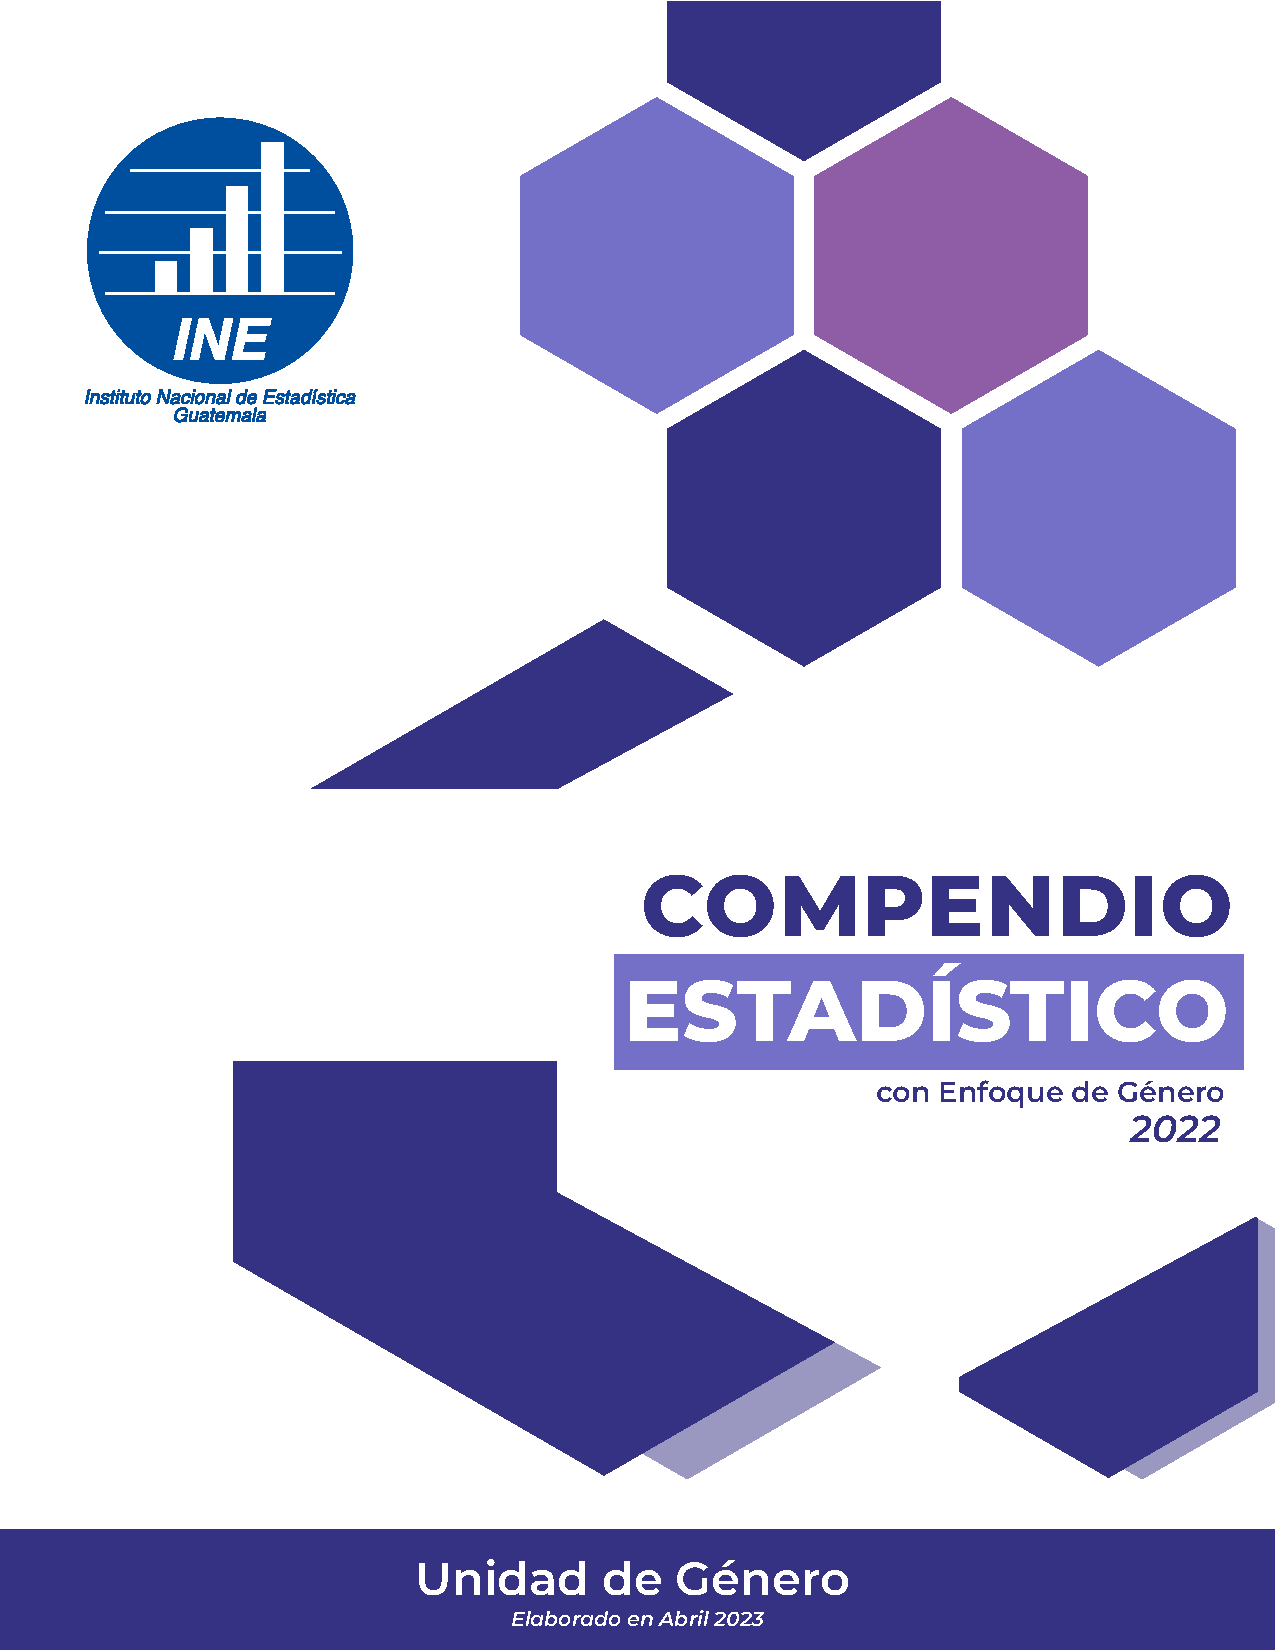
\includepdf{Plantilla/Portada_CEEG_2022.pdf}
	\cleardoublepage
	\thispagestyle{soloarriba}
	\begin{center}
		{\Bold \LARGE AUTORIDADES}\\[1cm]
{\Bold \large \color{color3} JUNTA  DIRECTIVA} \\[0.4cm]
{\Bold Ministerio de Economía}\\ 
Titular: Janio Moacyr Rosales Alegría \\ 
Suplente: Francisca de Jesús Cárdenas Morán\\[0.4cm]

{\Bold Ministerio de Finanzas Públicas}\\ 
Titular: Edwin Oswaldo Martínez Cameros\\ 
Suplente: José Hugo Valle Alegría\\[0.4cm]

{\Bold Ministerio de Agricultura, Ganadería y Alimentación}\\ 
Titular: Edgar René De León Moreno\\ 
Suplente: César Vinicio Arreaga Morales\\[0.4cm]

{\Bold Ministerio de Energía y Minas}\\ 
Titular: Alberto Pimentel Mata\\ 
Suplente: Oscar Rafael Pérez Ramírez\\[0.4cm]

{\Bold Secretaría de Planificación y Programación de la Presidencia}\\ 
Titular: Luz Keila Virginia Gramajo Vilchez\\ 
Suplente: Manuel Augusto Alonzo Araujo\\[0.4cm]

{\Bold Banco de Guatemala}\\ 
Titular: Álvaro González Ricci \\ 
Suplente: José Alfredo Blanco Valdés\\[0.4cm]

{\Bold Universidad de San Carlos de Guatemala}\\ 
Titular: Sindy Massiel Godínez Bautista\\ 
Suplente: José Lara Samayoa\\[0.4cm]

{\Bold Universidades Privadas}\\ 
Titular: Miguel Ángel Franco de León\\ 
Suplente: Oscar Leonel Herrera Velásquez\\[0.4cm]

{\Bold Comité Coordinador de Asociaciones Agrícolas, Comerciales, Industriales y Financieras}\\ 
Titular: Hugo Leonel Maúl Rivas\\ 
Suplente: Ricardo Antonio Rodríguez Martínez\\[0.4cm]

{\Bold \large \color{color3} GERENCIA}\\[0.2cm]
Gerente: Brenda Izabel Miranda Consuegra\\ 
Subgerente Técnico: Hugo Allan García Monterrosa\\ 
Subgerente Administrativo Financiero: Marco Antonio Mejía Villatoro\\ 

	\end{center}
	\cleardoublepage
	$\ $
	\vspace{0.0cm}
	\thispagestyle{soloarriba}
	\begin{center}
		{\Bold \LARGE EQUIPO RESPONSABLE}\\[2cm]
%{\Bold \large \color{color1!89!black} REVISIÓN GENERAL}\\[0.2cm]
%Brenda Izabel Miranda Consuegra\\[0.8cm]
{\Bold \large \color{color1!89!black} EQUIPO TÉCNICO}\\[0.2cm]
Brenda Izabel Miranda Consuegra\\
Hugo Allan García Monterrosa\\
Edgar Edwardo Herrarte Rodríguez\\
Julio Roberto Ramírez Pacheco \\
Luis Fernando Castellanos Bonilla \\
María Eugenia Guzmán Chete\\
Cristian Miguel Cabrera Ayala\\
Marvin Isaac Reyes López\\
Patricia Eugenia Hernandez García\\
Paula Natalia Gálvez Molina\\
Rodrigo Rafael Castillo Chong\\
Gerardo Ernesto Rodríguez\\
Mario Raul Soto Gómez\\
Luis Alberto Peñate López\\[0.8cm]
{\Bold \large \color{color1!89!black} DIAGRAMACIÓN Y DISEÑO}\\[0.2cm]
Andrea Michelle Rojas Salvatierra\\[0.8cm]

	\end{center}
	\cleardoublepage
	$\ $
	\vspace{0.0cm}
	\thispagestyle{soloarriba}
	\begin{center}
{\Bold \LARGE \color{color3} PRESENTACIÓN}\\[2cm]
\end{center}

EN PROCESO
\begin{center}
Brenda Izabel Miranda Consuegra\\
\textbf{Gerente}
\end{center}


	\cleardoublepage
	$\ $\\[2cm]
	\tableofcontents
	\pagestyle{estandar}	
	\vspace{0.0cm}
	\clearpage
	\setcounter{page}{0}
	
	\INEchaptercarta{Población y demografía}{Capítulo dedicado a mostrar una composición general de las personas que habitan en el territorio guatemalteco respecto al tamaño y la estructura de la población diferenciada por sexo, por edad, contribuyendo a la construcción de indicadores de la dinámica demográfica, a nivel nacional con un enfoque de género y pueblos.}
	\cajota{Población por sexo, según grupos de edad}{Para el 2022, el grupo de edad de 15 a 19 años tiene la población más grande de los grupos de edad con 956,598.8 miles de personas. El siguiente grupo más poblado es de 0 a 4 años de edad con 1681.9 miles de personas. Por el contrario,  la población de 100 años o más cuenta con la menor cantidad de personas de todos los grupos con 1.2 miles de personas. }{Población por sexo, según grupos de edad (miles de personas), 2022}{República de Guatemala, Instituto Nacional de Estadística}{\begin{tikzpicture}[x=1pt,y=1pt, scale=1.75]% Created by tikzDevice version 0.12.4 on 2023-04-04 13:49:55
% !TEX encoding = UTF-8 Unicode
\definecolor{fillColor}{RGB}{255,255,255}
\path[use as bounding box,fill=fillColor,fill opacity=0.00] (0,0) rectangle (289.08,198.74);
\begin{scope}
\path[clip] (  0.00,  0.00) rectangle (289.08,198.74);
\definecolor{drawColor}{RGB}{255,255,255}
\definecolor{fillColor}{RGB}{255,255,255}

\path[draw=drawColor,line width= 0.6pt,line join=round,line cap=round,fill=fillColor] (  0.00,  0.00) rectangle (289.08,198.74);
\end{scope}
\begin{scope}
\path[clip] (  0.00,  0.00) rectangle (289.08,198.74);
\definecolor{fillColor}{RGB}{54,50,131}

\path[fill=fillColor] ( 49.83, 33.17) rectangle (128.50, 40.01);

\path[fill=fillColor] ( 50.06, 40.77) rectangle (128.50, 47.62);

\path[fill=fillColor] ( 53.08, 48.38) rectangle (128.50, 55.22);

\path[fill=fillColor] ( 47.93, 55.98) rectangle (128.50, 62.83);

\path[fill=fillColor] ( 55.37, 63.59) rectangle (128.50, 70.43);

\path[fill=fillColor] ( 66.82, 71.19) rectangle (128.50, 78.03);

\path[fill=fillColor] ( 77.71, 78.79) rectangle (128.50, 85.64);

\path[fill=fillColor] ( 81.13, 86.40) rectangle (128.50, 93.24);

\path[fill=fillColor] ( 90.24, 94.00) rectangle (128.50,100.85);

\path[fill=fillColor] ( 96.76,101.61) rectangle (128.50,108.45);

\path[fill=fillColor] (101.65,109.21) rectangle (128.50,116.06);

\path[fill=fillColor] (105.47,116.82) rectangle (128.50,123.66);

\path[fill=fillColor] (109.95,124.42) rectangle (128.50,131.27);

\path[fill=fillColor] (113.42,132.03) rectangle (128.50,138.87);

\path[fill=fillColor] (118.19,139.63) rectangle (128.50,146.47);

\path[fill=fillColor] (121.23,147.24) rectangle (128.50,154.08);

\path[fill=fillColor] (123.82,154.84) rectangle (128.50,161.68);

\path[fill=fillColor] (125.59,162.44) rectangle (128.50,169.29);

\path[fill=fillColor] (127.43,170.05) rectangle (128.50,176.89);

\path[fill=fillColor] (128.15,177.65) rectangle (128.50,184.50);

\path[fill=fillColor] (128.43,185.26) rectangle (128.50,192.10);
\definecolor{fillColor}{RGB}{116,112,200}

\path[fill=fillColor] (128.50, 33.17) rectangle (208.89, 40.01);

\path[fill=fillColor] (128.50, 40.77) rectangle (208.64, 47.62);

\path[fill=fillColor] (128.50, 48.38) rectangle (205.73, 55.22);

\path[fill=fillColor] (128.50, 55.98) rectangle (207.08, 62.83);

\path[fill=fillColor] (128.50, 63.59) rectangle (196.62, 70.43);

\path[fill=fillColor] (128.50, 71.19) rectangle (183.82, 78.03);

\path[fill=fillColor] (128.50, 78.79) rectangle (173.20, 85.64);

\path[fill=fillColor] (128.50, 86.40) rectangle (169.09, 93.24);

\path[fill=fillColor] (128.50, 94.00) rectangle (162.08,100.85);

\path[fill=fillColor] (128.50,101.61) rectangle (155.53,108.45);

\path[fill=fillColor] (128.50,109.21) rectangle (152.06,116.06);

\path[fill=fillColor] (128.50,116.82) rectangle (148.32,123.66);

\path[fill=fillColor] (128.50,124.42) rectangle (145.04,131.27);

\path[fill=fillColor] (128.50,132.03) rectangle (141.84,138.87);

\path[fill=fillColor] (128.50,139.63) rectangle (138.12,146.47);

\path[fill=fillColor] (128.50,147.24) rectangle (135.12,154.08);

\path[fill=fillColor] (128.50,154.84) rectangle (132.74,161.68);

\path[fill=fillColor] (128.50,162.44) rectangle (130.97,169.29);

\path[fill=fillColor] (128.50,170.05) rectangle (129.36,176.89);

\path[fill=fillColor] (128.50,177.65) rectangle (128.75,184.50);

\path[fill=fillColor] (128.50,185.26) rectangle (128.54,192.10);
\end{scope}
\begin{scope}
\path[clip] (  0.00,  0.00) rectangle (289.08,198.74);
\definecolor{drawColor}{gray}{0.30}

\node[text=drawColor,anchor=base east,inner sep=0pt, outer sep=0pt, scale=  0.80] at ( 34.93, 33.46) {0-4};

\node[text=drawColor,anchor=base east,inner sep=0pt, outer sep=0pt, scale=  0.80] at ( 34.93, 41.07) {5-9};

\node[text=drawColor,anchor=base east,inner sep=0pt, outer sep=0pt, scale=  0.80] at ( 34.93, 48.67) {10-14};

\node[text=drawColor,anchor=base east,inner sep=0pt, outer sep=0pt, scale=  0.80] at ( 34.93, 56.28) {15-19};

\node[text=drawColor,anchor=base east,inner sep=0pt, outer sep=0pt, scale=  0.80] at ( 34.93, 63.88) {20-24};

\node[text=drawColor,anchor=base east,inner sep=0pt, outer sep=0pt, scale=  0.80] at ( 34.93, 71.49) {25-29};

\node[text=drawColor,anchor=base east,inner sep=0pt, outer sep=0pt, scale=  0.80] at ( 34.93, 79.09) {30-34};

\node[text=drawColor,anchor=base east,inner sep=0pt, outer sep=0pt, scale=  0.80] at ( 34.93, 86.69) {35-39};

\node[text=drawColor,anchor=base east,inner sep=0pt, outer sep=0pt, scale=  0.80] at ( 34.93, 94.30) {40-44};

\node[text=drawColor,anchor=base east,inner sep=0pt, outer sep=0pt, scale=  0.80] at ( 34.93,101.90) {45-49};

\node[text=drawColor,anchor=base east,inner sep=0pt, outer sep=0pt, scale=  0.80] at ( 34.93,109.51) {50-54};

\node[text=drawColor,anchor=base east,inner sep=0pt, outer sep=0pt, scale=  0.80] at ( 34.93,117.11) {55-59};

\node[text=drawColor,anchor=base east,inner sep=0pt, outer sep=0pt, scale=  0.80] at ( 34.93,124.72) {60-64};

\node[text=drawColor,anchor=base east,inner sep=0pt, outer sep=0pt, scale=  0.80] at ( 34.93,132.32) {65-69};

\node[text=drawColor,anchor=base east,inner sep=0pt, outer sep=0pt, scale=  0.80] at ( 34.93,139.93) {70-74};

\node[text=drawColor,anchor=base east,inner sep=0pt, outer sep=0pt, scale=  0.80] at ( 34.93,147.53) {75-79};

\node[text=drawColor,anchor=base east,inner sep=0pt, outer sep=0pt, scale=  0.80] at ( 34.93,155.14) {80-84};

\node[text=drawColor,anchor=base east,inner sep=0pt, outer sep=0pt, scale=  0.80] at ( 34.93,162.74) {85-89};

\node[text=drawColor,anchor=base east,inner sep=0pt, outer sep=0pt, scale=  0.80] at ( 34.93,170.34) {90-94};

\node[text=drawColor,anchor=base east,inner sep=0pt, outer sep=0pt, scale=  0.80] at ( 34.93,177.95) {95-99};

\node[text=drawColor,anchor=base east,inner sep=0pt, outer sep=0pt, scale=  0.80] at ( 34.93,185.55) {100+};
\end{scope}
\begin{scope}
\path[clip] (  0.00,  0.00) rectangle (289.08,198.74);
\definecolor{drawColor}{gray}{0.20}

\path[draw=drawColor,line width= 0.6pt,line join=round] ( 37.13, 36.59) --
	( 39.88, 36.59);

\path[draw=drawColor,line width= 0.6pt,line join=round] ( 37.13, 44.19) --
	( 39.88, 44.19);

\path[draw=drawColor,line width= 0.6pt,line join=round] ( 37.13, 51.80) --
	( 39.88, 51.80);

\path[draw=drawColor,line width= 0.6pt,line join=round] ( 37.13, 59.40) --
	( 39.88, 59.40);

\path[draw=drawColor,line width= 0.6pt,line join=round] ( 37.13, 67.01) --
	( 39.88, 67.01);

\path[draw=drawColor,line width= 0.6pt,line join=round] ( 37.13, 74.61) --
	( 39.88, 74.61);

\path[draw=drawColor,line width= 0.6pt,line join=round] ( 37.13, 82.22) --
	( 39.88, 82.22);

\path[draw=drawColor,line width= 0.6pt,line join=round] ( 37.13, 89.82) --
	( 39.88, 89.82);

\path[draw=drawColor,line width= 0.6pt,line join=round] ( 37.13, 97.43) --
	( 39.88, 97.43);

\path[draw=drawColor,line width= 0.6pt,line join=round] ( 37.13,105.03) --
	( 39.88,105.03);

\path[draw=drawColor,line width= 0.6pt,line join=round] ( 37.13,112.63) --
	( 39.88,112.63);

\path[draw=drawColor,line width= 0.6pt,line join=round] ( 37.13,120.24) --
	( 39.88,120.24);

\path[draw=drawColor,line width= 0.6pt,line join=round] ( 37.13,127.84) --
	( 39.88,127.84);

\path[draw=drawColor,line width= 0.6pt,line join=round] ( 37.13,135.45) --
	( 39.88,135.45);

\path[draw=drawColor,line width= 0.6pt,line join=round] ( 37.13,143.05) --
	( 39.88,143.05);

\path[draw=drawColor,line width= 0.6pt,line join=round] ( 37.13,150.66) --
	( 39.88,150.66);

\path[draw=drawColor,line width= 0.6pt,line join=round] ( 37.13,158.26) --
	( 39.88,158.26);

\path[draw=drawColor,line width= 0.6pt,line join=round] ( 37.13,165.87) --
	( 39.88,165.87);

\path[draw=drawColor,line width= 0.6pt,line join=round] ( 37.13,173.47) --
	( 39.88,173.47);

\path[draw=drawColor,line width= 0.6pt,line join=round] ( 37.13,181.08) --
	( 39.88,181.08);

\path[draw=drawColor,line width= 0.6pt,line join=round] ( 37.13,188.68) --
	( 39.88,188.68);
\end{scope}
\begin{scope}
\path[clip] (  0.00,  0.00) rectangle (289.08,198.74);
\definecolor{drawColor}{gray}{0.20}

\path[draw=drawColor,line width= 0.6pt,line join=round] ( 47.93, 29.28) --
	( 47.93, 32.03);

\path[draw=drawColor,line width= 0.6pt,line join=round] ( 88.21, 29.28) --
	( 88.21, 32.03);

\path[draw=drawColor,line width= 0.6pt,line join=round] (128.50, 29.28) --
	(128.50, 32.03);

\path[draw=drawColor,line width= 0.6pt,line join=round] (168.69, 29.28) --
	(168.69, 32.03);

\path[draw=drawColor,line width= 0.6pt,line join=round] (208.89, 29.28) --
	(208.89, 32.03);
\end{scope}
\begin{scope}
\path[clip] (  0.00,  0.00) rectangle (289.08,198.74);
\definecolor{drawColor}{gray}{0.30}

\node[text=drawColor,anchor=base,inner sep=0pt, outer sep=0pt, scale=  0.80] at ( 47.93, 20.82) {851.9};

\node[text=drawColor,anchor=base,inner sep=0pt, outer sep=0pt, scale=  0.80] at ( 88.21, 20.82) {426};

\node[text=drawColor,anchor=base,inner sep=0pt, outer sep=0pt, scale=  0.80] at (128.50, 20.82) {0};

\node[text=drawColor,anchor=base,inner sep=0pt, outer sep=0pt, scale=  0.80] at (168.69, 20.82) {425};

\node[text=drawColor,anchor=base,inner sep=0pt, outer sep=0pt, scale=  0.80] at (208.89, 20.82) {850.1};
\end{scope}
\begin{scope}
\path[clip] (  0.00,  0.00) rectangle (289.08,198.74);
\definecolor{drawColor}{RGB}{0,0,0}

\node[text=drawColor,anchor=base,inner sep=0pt, outer sep=0pt, scale=  1.00] at (128.41,  8.14) {Población en miles de personas};
\end{scope}
\begin{scope}
\path[clip] (  0.00,  0.00) rectangle (289.08,198.74);
\definecolor{drawColor}{RGB}{0,0,0}

\node[text=drawColor,rotate= 90.00,anchor=base,inner sep=0pt, outer sep=0pt, scale=  1.00] at ( 13.32,112.63) {Grupo de edad};
\end{scope}
\begin{scope}
\path[clip] (  0.00,  0.00) rectangle (289.08,198.74);
\definecolor{fillColor}{RGB}{255,255,255}

\path[fill=fillColor] (227.94, 83.26) rectangle (283.58,142.01);
\end{scope}
\begin{scope}
\path[clip] (  0.00,  0.00) rectangle (289.08,198.74);
\definecolor{drawColor}{RGB}{0,0,0}

\node[text=drawColor,anchor=base west,inner sep=0pt, outer sep=0pt, scale=  1.00] at (233.44,127.38) {Sexo};
\end{scope}
\begin{scope}
\path[clip] (  0.00,  0.00) rectangle (289.08,198.74);
\definecolor{fillColor}{gray}{0.95}

\path[fill=fillColor] (233.44,104.66) rectangle (249.34,120.55);
\end{scope}
\begin{scope}
\path[clip] (  0.00,  0.00) rectangle (289.08,198.74);
\definecolor{fillColor}{RGB}{54,50,131}

\path[fill=fillColor] (234.15,105.37) rectangle (248.63,119.84);
\end{scope}
\begin{scope}
\path[clip] (  0.00,  0.00) rectangle (289.08,198.74);
\definecolor{fillColor}{gray}{0.95}

\path[fill=fillColor] (233.44, 88.76) rectangle (249.34,104.66);
\end{scope}
\begin{scope}
\path[clip] (  0.00,  0.00) rectangle (289.08,198.74);
\definecolor{fillColor}{RGB}{116,112,200}

\path[fill=fillColor] (234.15, 89.47) rectangle (248.63,103.94);
\end{scope}
\begin{scope}
\path[clip] (  0.00,  0.00) rectangle (289.08,198.74);
\definecolor{drawColor}{RGB}{0,0,0}

\node[text=drawColor,anchor=base west,inner sep=0pt, outer sep=0pt, scale=  0.80] at (254.84,109.48) {Mujer};
\end{scope}
\begin{scope}
\path[clip] (  0.00,  0.00) rectangle (289.08,198.74);
\definecolor{drawColor}{RGB}{0,0,0}

\node[text=drawColor,anchor=base west,inner sep=0pt, outer sep=0pt, scale=  0.80] at (254.84, 93.58) {Hombre};
\end{scope}
\end{tikzpicture}}{INE - Proyecciones 2020} %1

\cajita{Población por sexo, según dominio de estudio}{Para 2022, según las proyecciones de población del Instituto Nacional de Estadística, en la República de Guatemala habitaban 17,357,886 personas. }{Población por sexo, según dominio de estudio (porcentaje), 2022}{República de Guatemala, Instituto Nacional de Estadística}{\begin{tikzpicture}[x=1pt,y=1pt, scale = 1.25]% Created by tikzDevice version 0.12.4 on 2023-04-20 12:31:17
% !TEX encoding = UTF-8 Unicode
\end{tikzpicture}}{INE - ENEI 2022}{} %2

\cajita{Población por sexo, según Pueblos}{Para 2022, el 31.2\% de la población guatemalteca estaba compuesta por mujeres ladinas. El 27.8\% eran hombres ladinos, y el 19.6\% mujeres mayas. El 0.1\% eran mujeres garífunas, otro 0.1\% hombres garífunas, y 0.1\% mujeres extranjeras. \footnote{Afrodescendiente*: Afrodescendiente/Creole/Afro mestizo.}}{Población por sexo, según Pueblos (porcentaje), 2022}{República de Guatemala, Instituto Nacional de Estadística}{\begin{tikzpicture}[x=1pt,y=1pt]% Created by tikzDevice version 0.12.4 on 2023-05-02 12:30:50
% !TEX encoding = UTF-8 Unicode
\definecolor{fillColor}{RGB}{255,255,255}
\path[use as bounding box,fill=fillColor,fill opacity=0.00] (0,0) rectangle (289.08,198.74);
\begin{scope}
\path[clip] (  0.00,  0.00) rectangle (289.08,198.74);

\path[] (  0.00,  0.00) rectangle (289.08,198.74);
\end{scope}
\begin{scope}
\path[clip] (  0.00,  0.00) rectangle (289.08,198.74);
\definecolor{fillColor}{RGB}{54,50,131}

\path[fill=fillColor] ( 80.50,171.20) rectangle ( 85.23,183.01);

\path[fill=fillColor] ( 80.50, 92.52) rectangle ( 81.24,104.32);

\path[fill=fillColor] ( 80.50,118.75) rectangle (279.15,130.55);

\path[fill=fillColor] ( 80.50, 40.07) rectangle ( 88.59, 51.87);

\path[fill=fillColor] ( 80.50, 66.29) rectangle ( 81.13, 78.10);

\path[fill=fillColor] ( 80.50,144.98) rectangle (205.38,156.78);
\definecolor{fillColor}{RGB}{116,112,200}

\path[fill=fillColor] ( 80.50,183.01) rectangle ( 84.35,194.81);

\path[fill=fillColor] ( 80.50,104.32) rectangle ( 81.11,116.13);

\path[fill=fillColor] ( 80.50,130.55) rectangle (257.44,142.35);

\path[fill=fillColor] ( 80.50, 51.87) rectangle ( 89.16, 63.67);

\path[fill=fillColor] ( 80.50, 78.10) rectangle ( 81.45, 89.90);

\path[fill=fillColor] ( 80.50,156.78) rectangle (188.23,168.58);
\definecolor{drawColor}{RGB}{0,0,0}

\node[text=drawColor,anchor=base west,inner sep=0pt, outer sep=0pt, scale=  0.68] at ( 89.50,173.42) {0.7};

\node[text=drawColor,anchor=base west,inner sep=0pt, outer sep=0pt, scale=  0.68] at ( 85.51, 94.73) {0.1};

\node[text=drawColor,anchor=base west,inner sep=0pt, outer sep=0pt, scale=  0.68] at (279.12,120.96) {31.2};

\node[text=drawColor,anchor=base west,inner sep=0pt, outer sep=0pt, scale=  0.63] at ( 92.86, 42.28) {1.3};

\node[text=drawColor,anchor=base west,inner sep=0pt, outer sep=0pt, scale=  0.63] at ( 85.40, 68.51) {0.1};

\node[text=drawColor,anchor=base west,inner sep=0pt, outer sep=0pt, scale=  0.63] at (211.36,147.19) {19.6};

\node[text=drawColor,anchor=base west,inner sep=0pt, outer sep=0pt, scale=  0.63] at ( 88.62,186.53) {0.6};

\node[text=drawColor,anchor=base west,inner sep=0pt, outer sep=0pt, scale=  0.63] at ( 85.38,107.85) {0.1};

\node[text=drawColor,anchor=base west,inner sep=0pt, outer sep=0pt, scale=  0.63] at (263.41,134.07) {27.8};

\node[text=drawColor,anchor=base west,inner sep=0pt, outer sep=0pt, scale=  0.63] at ( 93.44, 55.39) {1.4};

\node[text=drawColor,anchor=base west,inner sep=0pt, outer sep=0pt, scale=  0.63] at ( 85.73, 81.62) {0.2};

\node[text=drawColor,anchor=base west,inner sep=0pt, outer sep=0pt, scale=  0.63] at (194.20,160.30) {16.9};

\path[] ( 70.56, 51.87) --
	(289.08, 51.87);

\path[] ( 70.56, 78.10) --
	(289.08, 78.10);

\path[] ( 70.56,104.32) --
	(289.08,104.32);

\path[] ( 70.56,130.55) --
	(289.08,130.55);

\path[] ( 70.56,156.78) --
	(289.08,156.78);

\path[] ( 70.56,183.01) --
	(289.08,183.01);

\path[] ( 70.56, 36.13) rectangle (289.08,198.74);
\end{scope}
\begin{scope}
\path[clip] (  0.00,  0.00) rectangle (289.08,198.74);

\path[] ( 70.56, 36.13) --
	( 70.56,198.74);
\end{scope}
\begin{scope}
\path[clip] (  0.00,  0.00) rectangle (289.08,198.74);
\definecolor{drawColor}{RGB}{0,0,0}

\node[text=drawColor,anchor=base east,inner sep=0pt, outer sep=0pt, scale=  1.00] at ( 65.61, 47.96) {Afrodescendiente*};

\node[text=drawColor,anchor=base east,inner sep=0pt, outer sep=0pt, scale=  1.00] at ( 65.61, 74.19) {Extranjero};

\node[text=drawColor,anchor=base east,inner sep=0pt, outer sep=0pt, scale=  1.00] at ( 65.61,100.41) {Garífuna};

\node[text=drawColor,anchor=base east,inner sep=0pt, outer sep=0pt, scale=  1.00] at ( 65.61,126.64) {Ladino};

\node[text=drawColor,anchor=base east,inner sep=0pt, outer sep=0pt, scale=  1.00] at ( 65.61,152.87) {Maya};

\node[text=drawColor,anchor=base east,inner sep=0pt, outer sep=0pt, scale=  1.00] at ( 65.61,179.10) {Xinka};
\end{scope}
\begin{scope}
\path[clip] (  0.00,  0.00) rectangle (289.08,198.74);

\path[] ( 67.81, 51.87) --
	( 70.56, 51.87);

\path[] ( 67.81, 78.10) --
	( 70.56, 78.10);

\path[] ( 67.81,104.32) --
	( 70.56,104.32);

\path[] ( 67.81,130.55) --
	( 70.56,130.55);

\path[] ( 67.81,156.78) --
	( 70.56,156.78);

\path[] ( 67.81,183.01) --
	( 70.56,183.01);
\end{scope}
\begin{scope}
\path[clip] (  0.00,  0.00) rectangle (289.08,198.74);

\path[] ( 70.56, 36.13) --
	(289.08, 36.13);
\end{scope}
\begin{scope}
\path[clip] (  0.00,  0.00) rectangle (289.08,198.74);

\path[] ( 80.50, 33.38) --
	( 80.50, 36.13);

\path[] (144.15, 33.38) --
	(144.15, 36.13);

\path[] (207.80, 33.38) --
	(207.80, 36.13);

\path[] (271.45, 33.38) --
	(271.45, 36.13);
\end{scope}
\begin{scope}
\path[clip] (  0.00,  0.00) rectangle (289.08,198.74);
\definecolor{fillColor}{RGB}{255,255,255}

\path[fill=fillColor] (131.74, -0.00) rectangle (227.91, 22.38);
\end{scope}
\begin{scope}
\path[clip] (  0.00,  0.00) rectangle (289.08,198.74);
\definecolor{fillColor}{gray}{0.95}

\path[fill=fillColor] (132.74,  5.50) rectangle (144.12, 16.88);
\end{scope}
\begin{scope}
\path[clip] (  0.00,  0.00) rectangle (289.08,198.74);
\definecolor{fillColor}{RGB}{54,50,131}

\path[fill=fillColor] (133.40,  6.16) rectangle (143.46, 16.22);  %cuadro leyenda mujeres
\end{scope}
\begin{scope}
\path[clip] (  0.00,  0.00) rectangle (289.08,198.74);
\definecolor{fillColor}{gray}{0.95}

\path[fill=fillColor] (182.28,  5.50) rectangle (193.66, 16.88);
\end{scope}
\begin{scope}
\path[clip] (  0.00,  0.00) rectangle (289.08,198.74);
\definecolor{fillColor}{RGB}{116,112,200}

\path[fill=fillColor] (182.94,  6.16) rectangle (193.00, 16.22);
\end{scope}
\begin{scope}
\path[clip] (  0.00,  0.00) rectangle (289.08,198.74);
\definecolor{drawColor}{RGB}{0,0,0}

\node[text=drawColor,anchor=base west,inner sep=0pt, outer sep=0pt, scale=  0.80] at (149.62,  8.06) {Mujeres};
\end{scope}
\begin{scope}
\path[clip] (  0.00,  0.00) rectangle (289.08,198.74);
\definecolor{drawColor}{RGB}{0,0,0}

\node[text=drawColor,anchor=base west,inner sep=0pt, outer sep=0pt, scale=  0.80] at (199.16,  8.06) {Hombres};
\end{scope}
\end{tikzpicture}}{INE - ENEI 2022}{} %3

\cajota{Población por sexo, según comunidad lingüística}{Para el 2018, se muestra el número de personas por sexo pertenecientes a las 22 comunidades lingüísticas Maya. Se observa que en la mayoría de comunidades existe una mayor población de mujeres, con excepción de la comunidad Itza’.}{Población por sexo, según comunidad lingüística (número de personas), 2018}{República de Guatemala, Instituto Nacional de Estadística}{\begin{tikzpicture}[x=1pt,y=1pt, scale=1.75]% Created by tikzDevice version 0.12.4 on 2023-05-08 10:54:28
% !TEX encoding = UTF-8 Unicode
\definecolor{fillColor}{RGB}{255,255,255}
\path[use as bounding box,fill=fillColor,fill opacity=0.00] (0,0) rectangle (289.08,198.74);
\begin{scope}
\path[clip] (  0.00,  0.00) rectangle (289.08,198.74);
\definecolor{drawColor}{RGB}{255,255,255}
\definecolor{fillColor}{RGB}{255,255,255}

\path[draw=drawColor,line width= 0.6pt,line join=round,line cap=round,fill=fillColor] (  0.00,  0.00) rectangle (289.08,198.74);
\end{scope}
\begin{scope}
\path[clip] (  0.00,  0.00) rectangle (289.08,198.74);
\definecolor{fillColor}{RGB}{54,50,131}

\path[fill=fillColor] (134.05,  6.77) rectangle (213.87, 14.38);

\path[fill=fillColor] (137.61, 15.23) rectangle (213.87, 22.84);

\path[fill=fillColor] (131.67, 23.68) rectangle (213.87, 31.29);

\path[fill=fillColor] (136.88, 32.14) rectangle (213.87, 39.75);

\path[fill=fillColor] (133.91, 40.60) rectangle (213.87, 48.21);

\path[fill=fillColor] (135.04, 49.05) rectangle (213.87, 56.66);

\path[fill=fillColor] (141.56, 57.51) rectangle (213.87, 65.12);

\path[fill=fillColor] (134.14, 65.97) rectangle (213.87, 73.58);

\path[fill=fillColor] (132.55, 74.42) rectangle (213.87, 82.03);

\path[fill=fillColor] (134.24, 82.88) rectangle (213.87, 90.49);

\path[fill=fillColor] (136.05, 91.34) rectangle (213.87, 98.95);

\path[fill=fillColor] (133.87, 99.79) rectangle (213.87,107.41);

\path[fill=fillColor] (137.35,108.25) rectangle (213.87,115.86);

\path[fill=fillColor] (135.08,116.71) rectangle (213.87,124.32);

\path[fill=fillColor] (137.45,125.16) rectangle (213.87,132.78);

\path[fill=fillColor] (134.62,133.62) rectangle (213.87,141.23);

\path[fill=fillColor] (137.98,142.08) rectangle (213.87,149.69);

\path[fill=fillColor] (133.67,150.54) rectangle (213.87,158.15);

\path[fill=fillColor] (136.52,158.99) rectangle (213.87,166.60);

\path[fill=fillColor] (135.40,167.45) rectangle (213.87,175.06);

\path[fill=fillColor] (137.08,175.91) rectangle (213.87,183.52);

\path[fill=fillColor] (134.83,184.36) rectangle (213.87,191.97);
\definecolor{fillColor}{RGB}{116,112,200}

\path[fill=fillColor] ( 62.19,  6.77) rectangle (134.05, 14.38);

\path[fill=fillColor] ( 62.19, 15.23) rectangle (137.61, 22.84);

\path[fill=fillColor] ( 62.19, 23.68) rectangle (131.67, 31.29);

\path[fill=fillColor] ( 62.19, 32.14) rectangle (136.88, 39.75);

\path[fill=fillColor] ( 62.19, 40.60) rectangle (133.91, 48.21);

\path[fill=fillColor] ( 62.19, 49.05) rectangle (135.04, 56.66);

\path[fill=fillColor] ( 62.19, 57.51) rectangle (141.56, 65.12);

\path[fill=fillColor] ( 62.19, 65.97) rectangle (134.14, 73.58);

\path[fill=fillColor] ( 62.19, 74.42) rectangle (132.55, 82.03);

\path[fill=fillColor] ( 62.19, 82.88) rectangle (134.24, 90.49);

\path[fill=fillColor] ( 62.19, 91.34) rectangle (136.05, 98.95);

\path[fill=fillColor] ( 62.19, 99.79) rectangle (133.87,107.41);

\path[fill=fillColor] ( 62.19,108.25) rectangle (137.35,115.86);

\path[fill=fillColor] ( 62.19,116.71) rectangle (135.08,124.32);

\path[fill=fillColor] ( 62.19,125.16) rectangle (137.45,132.78);

\path[fill=fillColor] ( 62.19,133.62) rectangle (134.62,141.23);

\path[fill=fillColor] ( 62.19,142.08) rectangle (137.98,149.69);

\path[fill=fillColor] ( 62.19,150.54) rectangle (133.67,158.15);

\path[fill=fillColor] ( 62.19,158.99) rectangle (136.52,166.60);

\path[fill=fillColor] ( 62.19,167.45) rectangle (135.40,175.06);

\path[fill=fillColor] ( 62.19,175.91) rectangle (137.08,183.52);

\path[fill=fillColor] ( 62.19,184.36) rectangle (134.83,191.97);
\definecolor{drawColor}{RGB}{255,255,255}

\node[text=drawColor,anchor=base,inner sep=0pt, outer sep=0pt, scale=  0.78] at (173.96,  7.54) {84,649};

\node[text=drawColor,anchor=base,inner sep=0pt, outer sep=0pt, scale=  0.78] at (175.74, 16.00) {33,167};

\node[text=drawColor,anchor=base,inner sep=0pt, outer sep=0pt, scale=  0.78] at (172.77, 24.45) {6,796};

\node[text=drawColor,anchor=base,inner sep=0pt, outer sep=0pt, scale=  0.78] at (175.37, 32.91) {57,071};

\node[text=drawColor,anchor=base,inner sep=0pt, outer sep=0pt, scale=  0.78] at (173.89, 41.37) {17,735};

\node[text=drawColor,anchor=base,inner sep=0pt, outer sep=0pt, scale=  0.78] at (174.46, 49.83) {47,496};

\node[text=drawColor,anchor=base,inner sep=0pt, outer sep=0pt, scale=  0.78] at (177.71, 58.28) {1,395};

\node[text=drawColor,anchor=base,inner sep=0pt, outer sep=0pt, scale=  0.78] at (174.00, 66.74) {70,087};

\node[text=drawColor,anchor=base,inner sep=0pt, outer sep=0pt, scale=  0.78] at (173.21, 75.20) {29,077};

\node[text=drawColor,anchor=base,inner sep=0pt, outer sep=0pt, scale=  0.78] at (174.06, 83.65) {882,288};

\node[text=drawColor,anchor=base,inner sep=0pt, outer sep=0pt, scale=  0.78] at (174.96, 92.11) {548,134};

\node[text=drawColor,anchor=base,inner sep=0pt, outer sep=0pt, scale=  0.78] at (173.87,100.57) {444,217};

\node[text=drawColor,anchor=base,inner sep=0pt, outer sep=0pt, scale=  0.78] at (175.61,109.02) {1,695};

\node[text=drawColor,anchor=base,inner sep=0pt, outer sep=0pt, scale=  0.78] at (174.47,117.48) {24,144};

\node[text=drawColor,anchor=base,inner sep=0pt, outer sep=0pt, scale=  0.78] at (175.66,125.94) {88,987};

\node[text=drawColor,anchor=base,inner sep=0pt, outer sep=0pt, scale=  0.78] at (174.25,134.39) {108,680};

\node[text=drawColor,anchor=base,inner sep=0pt, outer sep=0pt, scale=  0.78] at (175.92,142.85) {685,495};

\node[text=drawColor,anchor=base,inner sep=0pt, outer sep=0pt, scale=  0.78] at (173.77,151.31) {6,841};

\node[text=drawColor,anchor=base,inner sep=0pt, outer sep=0pt, scale=  0.78] at (175.19,159.76) {8,860};

\node[text=drawColor,anchor=base,inner sep=0pt, outer sep=0pt, scale=  0.78] at (174.64,168.22) {1,716};

\node[text=drawColor,anchor=base,inner sep=0pt, outer sep=0pt, scale=  0.78] at (175.48,176.68) {53,668};

\node[text=drawColor,anchor=base,inner sep=0pt, outer sep=0pt, scale=  0.78] at (174.35,185.14) {2,558};

\node[text=drawColor,anchor=base,inner sep=0pt, outer sep=0pt, scale=  0.78] at ( 98.12,  7.54) {76,209};

\node[text=drawColor,anchor=base,inner sep=0pt, outer sep=0pt, scale=  0.78] at ( 99.90, 16.00) {32,798};

\node[text=drawColor,anchor=base,inner sep=0pt, outer sep=0pt, scale=  0.78] at ( 96.93, 24.45) {5,745};

\node[text=drawColor,anchor=base,inner sep=0pt, outer sep=0pt, scale=  0.78] at ( 99.53, 32.91) {55,361};

\node[text=drawColor,anchor=base,inner sep=0pt, outer sep=0pt, scale=  0.78] at ( 98.05, 41.37) {15,906};

\node[text=drawColor,anchor=base,inner sep=0pt, outer sep=0pt, scale=  0.78] at ( 98.62, 49.83) {43,895};

\node[text=drawColor,anchor=base,inner sep=0pt, outer sep=0pt, scale=  0.78] at (101.87, 58.28) {1,531};

\node[text=drawColor,anchor=base,inner sep=0pt, outer sep=0pt, scale=  0.78] at ( 98.16, 66.74) {63,242};

\node[text=drawColor,anchor=base,inner sep=0pt, outer sep=0pt, scale=  0.78] at ( 97.37, 75.20) {25,160};

\node[text=drawColor,anchor=base,inner sep=0pt, outer sep=0pt, scale=  0.78] at ( 98.21, 83.65) {798,263};

\node[text=drawColor,anchor=base,inner sep=0pt, outer sep=0pt, scale=  0.78] at ( 99.12, 92.11) {520,222};

\node[text=drawColor,anchor=base,inner sep=0pt, outer sep=0pt, scale=  0.78] at ( 98.03,100.57) {398,035};

\node[text=drawColor,anchor=base,inner sep=0pt, outer sep=0pt, scale=  0.78] at ( 99.77,109.02) {1,665};

\node[text=drawColor,anchor=base,inner sep=0pt, outer sep=0pt, scale=  0.78] at ( 98.63,117.48) {22,334};

\node[text=drawColor,anchor=base,inner sep=0pt, outer sep=0pt, scale=  0.78] at ( 99.82,125.94) {87,635};

\node[text=drawColor,anchor=base,inner sep=0pt, outer sep=0pt, scale=  0.78] at ( 98.40,134.39) {99,328};

\node[text=drawColor,anchor=base,inner sep=0pt, outer sep=0pt, scale=  0.78] at (100.08,142.85) {684,512};

\node[text=drawColor,anchor=base,inner sep=0pt, outer sep=0pt, scale=  0.78] at ( 97.93,151.31) {6,097};

\node[text=drawColor,anchor=base,inner sep=0pt, outer sep=0pt, scale=  0.78] at ( 99.35,159.76) {8,513};

\node[text=drawColor,anchor=base,inner sep=0pt, outer sep=0pt, scale=  0.78] at ( 98.80,168.22) {1,601};

\node[text=drawColor,anchor=base,inner sep=0pt, outer sep=0pt, scale=  0.78] at ( 99.64,176.68) {52,344};

\node[text=drawColor,anchor=base,inner sep=0pt, outer sep=0pt, scale=  0.78] at ( 98.51,185.14) {2,351};
\end{scope}
\begin{scope}
\path[clip] (  0.00,  0.00) rectangle (289.08,198.74);
\definecolor{drawColor}{RGB}{0,0,0}

\node[text=drawColor,anchor=base east,inner sep=0pt, outer sep=0pt, scale=  0.80] at ( 49.66,  7.45) {Achi};

\node[text=drawColor,anchor=base east,inner sep=0pt, outer sep=0pt, scale=  0.80] at ( 49.66, 15.90) {Akateka};

\node[text=drawColor,anchor=base east,inner sep=0pt, outer sep=0pt, scale=  0.80] at ( 49.66, 24.36) {Awakateka};

\node[text=drawColor,anchor=base east,inner sep=0pt, outer sep=0pt, scale=  0.80] at ( 49.66, 32.82) {Ch'orti'};

\node[text=drawColor,anchor=base east,inner sep=0pt, outer sep=0pt, scale=  0.80] at ( 49.66, 41.27) {Chalchiteka};

\node[text=drawColor,anchor=base east,inner sep=0pt, outer sep=0pt, scale=  0.80] at ( 49.66, 49.73) {Chuj};

\node[text=drawColor,anchor=base east,inner sep=0pt, outer sep=0pt, scale=  0.80] at ( 49.66, 58.19) {Itza'};

\node[text=drawColor,anchor=base east,inner sep=0pt, outer sep=0pt, scale=  0.80] at ( 49.66, 66.65) {Ixil};

\node[text=drawColor,anchor=base east,inner sep=0pt, outer sep=0pt, scale=  0.80] at ( 49.66, 75.10) {Jakalteko/Popti'};

\node[text=drawColor,anchor=base east,inner sep=0pt, outer sep=0pt, scale=  0.80] at ( 49.66, 83.56) {K'iche'};

\node[text=drawColor,anchor=base east,inner sep=0pt, outer sep=0pt, scale=  0.80] at ( 49.66, 92.02) {Kaqchiquel};

\node[text=drawColor,anchor=base east,inner sep=0pt, outer sep=0pt, scale=  0.80] at ( 49.66,100.47) {Mam};

\node[text=drawColor,anchor=base east,inner sep=0pt, outer sep=0pt, scale=  0.80] at ( 49.66,108.93) {Mopan};

\node[text=drawColor,anchor=base east,inner sep=0pt, outer sep=0pt, scale=  0.80] at ( 49.66,117.39) {Poqomam};

\node[text=drawColor,anchor=base east,inner sep=0pt, outer sep=0pt, scale=  0.80] at ( 49.66,125.84) {Poqomchi'};

\node[text=drawColor,anchor=base east,inner sep=0pt, outer sep=0pt, scale=  0.80] at ( 49.66,134.30) {Q'anjob'al};

\node[text=drawColor,anchor=base east,inner sep=0pt, outer sep=0pt, scale=  0.80] at ( 49.66,142.76) {Q'eqchi'};

\node[text=drawColor,anchor=base east,inner sep=0pt, outer sep=0pt, scale=  0.80] at ( 49.66,151.21) {Sakapulteka};

\node[text=drawColor,anchor=base east,inner sep=0pt, outer sep=0pt, scale=  0.80] at ( 49.66,159.67) {Sipakapense};

\node[text=drawColor,anchor=base east,inner sep=0pt, outer sep=0pt, scale=  0.80] at ( 49.66,168.13) {Tektiteka};

\node[text=drawColor,anchor=base east,inner sep=0pt, outer sep=0pt, scale=  0.80] at ( 49.66,176.58) {Tz'utujil};

\node[text=drawColor,anchor=base east,inner sep=0pt, outer sep=0pt, scale=  0.80] at ( 49.66,185.04) {Uspanteka};
\end{scope}
\begin{scope}
\path[clip] (  0.00,  0.00) rectangle (289.08,198.74);
\definecolor{fillColor}{RGB}{255,255,255}

\path[fill=fillColor] (232.46, 74.52) rectangle (283.58,124.23);
\end{scope}
\begin{scope}
\path[clip] (  0.00,  0.00) rectangle (289.08,198.74);
\definecolor{fillColor}{gray}{0.95}

%\path[fill=fillColor] (237.96, 91.40) rectangle (249.34,102.78);
\end{scope}
\begin{scope}
\path[clip] (  0.00,  0.00) rectangle (289.08,198.74);
\definecolor{fillColor}{RGB}{54,50,131}

\path[fill=fillColor] (240.62, 94.06) rectangle (248.67,102.12);
\end{scope}
\begin{scope}
\path[clip] (  0.00,  0.00) rectangle (289.08,198.74);
\definecolor{fillColor}{gray}{0.95}

%\path[fill=fillColor] (237.96, 80.02) rectangle (249.34, 91.40);
\end{scope}
\begin{scope}
\path[clip] (  0.00,  0.00) rectangle (289.08,198.74);
\definecolor{fillColor}{RGB}{116,112,200}

\path[fill=fillColor] (240.62, 84.68) rectangle (248.67, 92.74);
\end{scope}
\begin{scope}
\path[clip] (  0.00,  0.00) rectangle (289.08,198.74);
\definecolor{drawColor}{RGB}{0,0,0}

\node[text=drawColor,anchor=base west,inner sep=0pt, outer sep=0pt, scale=  0.80] at (254.84, 95.96) {Mujeres};
\end{scope}
\begin{scope}
\path[clip] (  0.00,  0.00) rectangle (289.08,198.74);
\definecolor{drawColor}{RGB}{0,0,0}

\node[text=drawColor,anchor=base west,inner sep=0pt, outer sep=0pt, scale=  0.80] at (254.84, 85.98) {Hombres};
\end{scope}
\end{tikzpicture}}{INE - Censo 2018} %4

\cajota{Población por sexo, según tipo de vivienda}{Para 2022, el 49.4\% de mujeres residía en casas formales al igual que el 43.4\%. Por el contrario, un 0.3\% de mujeres y un 0.3\% de hombres residían en ranchos.  }{Población por sexo, según tipo de vivienda (porcentaje), 2022}{República de Guatemala, Instituto Nacional de Estadística}{\begin{tikzpicture}[x=1pt,y=1pt, scale = 1.75]% Created by tikzDevice version 0.12.4 on 2023-04-25 12:07:28
% !TEX encoding = UTF-8 Unicode
\definecolor{fillColor}{RGB}{255,255,255}
\path[use as bounding box,fill=fillColor,fill opacity=0.00] (0,0) rectangle (289.08,198.74);
\begin{scope}
\path[clip] (  0.00,  0.00) rectangle (289.08,198.74);
\definecolor{drawColor}{RGB}{255,255,255}
\definecolor{fillColor}{RGB}{255,255,255}

\path[draw=drawColor,line width= 0.6pt,line join=round,line cap=round,fill=fillColor] (  0.00,  0.00) rectangle (289.08,198.74);
\end{scope}
\begin{scope}
\path[clip] (  0.00,  0.00) rectangle (289.08,198.74);
\definecolor{fillColor}{RGB}{54,50,131}

\path[fill=fillColor] (133.87, 47.02) rectangle (209.81, 79.51);

\path[fill=fillColor] (129.74, 10.92) rectangle (209.81, 43.41);

\path[fill=fillColor] (134.34,119.23) rectangle (209.81,151.72);

\path[fill=fillColor] (138.27,155.33) rectangle (209.81,187.83);

\path[fill=fillColor] (140.58, 83.12) rectangle (209.81,115.62);
\definecolor{fillColor}{RGB}{116,112,200}

\path[fill=fillColor] ( 67.17, 47.02) rectangle (133.87, 79.51);

\path[fill=fillColor] ( 67.17, 10.92) rectangle (129.74, 43.41);

\path[fill=fillColor] ( 67.17,119.23) rectangle (134.34,151.72);

\path[fill=fillColor] ( 67.17,155.33) rectangle (138.27,187.83);

\path[fill=fillColor] ( 67.17, 83.12) rectangle (140.58,115.62);
\definecolor{drawColor}{RGB}{255,255,255}

\node[text=drawColor,anchor=base,inner sep=0pt, outer sep=0pt, scale=  0.78] at (171.84, 60.23) {49.4};

\node[text=drawColor,anchor=base,inner sep=0pt, outer sep=0pt, scale=  0.78] at (169.77, 24.13) {0.9};

\node[text=drawColor,anchor=base,inner sep=0pt, outer sep=0pt, scale=  0.78] at (172.07,132.44) {0.3};

\node[text=drawColor,anchor=base,inner sep=0pt, outer sep=0pt, scale=  0.78] at (174.04,168.55) {0.7};

\node[text=drawColor,anchor=base,inner sep=0pt, outer sep=0pt, scale=  0.78] at (175.19, 96.34) {1.8};

\node[text=drawColor,anchor=base,inner sep=0pt, outer sep=0pt, scale=  0.78] at (100.52, 60.23) {43.4};

\node[text=drawColor,anchor=base,inner sep=0pt, outer sep=0pt, scale=  0.78] at ( 98.45, 24.13) {0.7};

\node[text=drawColor,anchor=base,inner sep=0pt, outer sep=0pt, scale=  0.78] at (100.75,132.44) {0.3};

\node[text=drawColor,anchor=base,inner sep=0pt, outer sep=0pt, scale=  0.78] at (102.72,168.55) {0.7};

\node[text=drawColor,anchor=base,inner sep=0pt, outer sep=0pt, scale=  0.78] at (103.87, 96.34) {2.0};
\end{scope}
\begin{scope}
\path[clip] (  0.00,  0.00) rectangle (289.08,198.74);
\definecolor{drawColor}{RGB}{0,0,0}

\node[text=drawColor,anchor=base east,inner sep=0pt, outer sep=0pt, scale=  0.80] at ( 55.08, 24.04) {Apartamento};

\node[text=drawColor,anchor=base east,inner sep=0pt, outer sep=0pt, scale=  0.80] at ( 55.08, 60.14) {Casa formal};

\node[text=drawColor,anchor=base east,inner sep=0pt, outer sep=0pt, scale=  0.80] at ( 55.08, 96.24) {Casa improvisada};

\node[text=drawColor,anchor=base east,inner sep=0pt, outer sep=0pt, scale=  0.80] at ( 55.08,132.35) {Cuarto vecindad};

\node[text=drawColor,anchor=base east,inner sep=0pt, outer sep=0pt, scale=  0.80] at ( 55.08,168.45) {Rancho};
\end{scope}
\begin{scope}
\path[clip] (  0.00,  0.00) rectangle (289.08,198.74);
\definecolor{fillColor}{RGB}{255,255,255}

\path[fill=fillColor] (227.94, 70.00) rectangle (283.58,128.74);
\end{scope}
\begin{scope}
\path[clip] (  0.00,  0.00) rectangle (289.08,198.74);
\definecolor{drawColor}{RGB}{0,0,0}

\node[text=drawColor,anchor=base west,inner sep=0pt, outer sep=0pt, scale=  1.00] at (233.44,114.11) {Sexo};
\end{scope}
\begin{scope}
\path[clip] (  0.00,  0.00) rectangle (289.08,198.74);
\definecolor{fillColor}{gray}{0.95}

\path[fill=fillColor] (233.44, 91.40) rectangle (249.34,107.30);
\end{scope}
\begin{scope}
\path[clip] (  0.00,  0.00) rectangle (289.08,198.74);
\definecolor{fillColor}{RGB}{54,50,131}

\path[fill=fillColor] (234.15, 92.11) rectangle (248.63,106.59);
\end{scope}
\begin{scope}
\path[clip] (  0.00,  0.00) rectangle (289.08,198.74);
\definecolor{fillColor}{gray}{0.95}

\path[fill=fillColor] (233.44, 75.50) rectangle (249.34, 91.40);
\end{scope}
\begin{scope}
\path[clip] (  0.00,  0.00) rectangle (289.08,198.74);
\definecolor{fillColor}{RGB}{116,112,200}

\path[fill=fillColor] (234.15, 76.21) rectangle (248.63, 90.69);
\end{scope}
\begin{scope}
\path[clip] (  0.00,  0.00) rectangle (289.08,198.74);
\definecolor{drawColor}{RGB}{0,0,0}

\node[text=drawColor,anchor=base west,inner sep=0pt, outer sep=0pt, scale=  0.80] at (254.84, 96.22) {Mujer};
\end{scope}
\begin{scope}
\path[clip] (  0.00,  0.00) rectangle (289.08,198.74);
\definecolor{drawColor}{RGB}{0,0,0}

\node[text=drawColor,anchor=base west,inner sep=0pt, outer sep=0pt, scale=  0.80] at (254.84, 80.32) {Hombre};
\end{scope}
\end{tikzpicture}}{INE - ENEI 2022} %5

\cajota{Mapa departamental por número de mujeres}{Este es un mapa departamental por sexo :)}{Proyección de población de mujeres por departamento (número de mujeres), 2022}{República de Guatemala, Instituto Nacional de Estadística}{\\[-0.5cm]\includegraphics[width=0.75\textwidth]{Graficas/mapa_departamental.png}}{INE - Proyecciones 2020} %6

\cajota{Mapa municipal por número de mujeres}{Para 2022, según estimaciones del Instituto Nacional de Estadística, el municipio con mayor población de mujeres fue el municipio de Guatemala con 630,634 mujeres, seguido de Mixco con 269,358 mujeres. Los municipios con menor proyección poblacional de mujeres fueron Santa María Visitación con 1,354 mujeres y San Marcos La Laguna con 1,531 mujeres.  }{Proyección de población de mujeres por municipio (número de mujeres), 2022}{República de Guatemala, Instituto Nacional de Estadística}{\\[-0.5cm]\includegraphics[width=0.75\textwidth]{Graficas/mapa_municipal.png}}{INE - Proyecciones 2020} %7

\cajita{Esperanza de vida al nacer por sexo}{La esperanza de vida al nacer indica la cantidad de años que se espera que viva la persona nacida en un periodo de tiempo determinado. En Guatemala, las mujeres tienen una esperanza de vida mayor que los hombres. El período de referencia es tomado hasta el 30 junio de cada año. }{Serie histórica de esperanza de vida (número de años), 2017-2022}{República de Guatemala, Instituto Nacional de Estadística, 2018 - 2021}{\begin{tikzpicture}[x=1pt,y=1pt]% Created by tikzDevice version 0.12.4 on 2023-05-15 10:48:14
% !TEX encoding = UTF-8 Unicode
\definecolor{fillColor}{RGB}{255,255,255}
\path[use as bounding box,fill=fillColor,fill opacity=0.00] (0,0) rectangle (289.08,198.74);
\begin{scope}
\path[clip] (  0.00,  0.00) rectangle (289.08,198.74);

\path[] (  0.00,  0.00) rectangle (289.08,198.74);
\end{scope}
\begin{scope}
\path[clip] (  0.00,  0.00) rectangle (289.08,198.74);
\definecolor{drawColor}{RGB}{54,50,131}

\path[draw=drawColor,line width= 1.7pt,line join=round] ( 31.91,128.88) --
	( 85.96,130.22) --
	(140.01,131.55) --
	(194.06,132.89) --
	(248.11,134.22);
\definecolor{drawColor}{RGB}{116,112,200}

\path[draw=drawColor,line width= 1.7pt,line join=round] ( 31.91, 85.49) --
	( 85.96, 86.82) --
	(140.01, 88.16) --
	(194.06, 89.49) --
	(248.11, 90.83);
\definecolor{drawColor}{RGB}{0,0,0}

\node[text=drawColor,anchor=base,inner sep=0pt, outer sep=0pt, scale=  1.02] at ( 31.91,116.97) {75.8};

\node[text=drawColor,anchor=base east,inner sep=0pt, outer sep=0pt, scale=  1.02] at ( 82.83,130.22) {76.0};

\node[text=drawColor,anchor=base east,inner sep=0pt, outer sep=0pt, scale=  1.02] at (136.88,131.55) {76.2};

\node[text=drawColor,anchor=base east,inner sep=0pt, outer sep=0pt, scale=  1.02] at (190.94,132.89) {76.4};

\node[text=drawColor,anchor=base,inner sep=0pt, outer sep=0pt, scale=  1.02] at (248.11,138.19) {76.6};

\node[text=drawColor,anchor=base,inner sep=0pt, outer sep=0pt, scale=  1.02] at ( 31.91, 73.58) {69.3};

\node[text=drawColor,anchor=base east,inner sep=0pt, outer sep=0pt, scale=  1.02] at ( 82.83, 86.82) {69.5};

\node[text=drawColor,anchor=base east,inner sep=0pt, outer sep=0pt, scale=  1.02] at (136.88, 88.16) {69.7};

\node[text=drawColor,anchor=base east,inner sep=0pt, outer sep=0pt, scale=  1.02] at (190.94, 89.49) {69.9};

\node[text=drawColor,anchor=base,inner sep=0pt, outer sep=0pt, scale=  1.02] at (248.11, 94.80) {70.1};

\path[draw=drawColor,line width= 0.1pt,line join=round] (-281.58, 23.41) -- (561.61, 23.41);

\path[] ( -0.52, 15.40) rectangle (280.54,191.63);

\path[] ( -0.52, 40.10) --
	(280.54, 40.10);

\path[] ( -0.52, 73.47) --
	(280.54, 73.47);

\path[] ( -0.52,106.85) --
	(280.54,106.85);

\path[] ( -0.52,140.23) --
	(280.54,140.23);

\path[] ( -0.52,173.61) --
	(280.54,173.61);

\path[] ( -0.52, 23.41) --
	(280.54, 23.41);

\path[] ( -0.52, 56.79) --
	(280.54, 56.79);

\path[] ( -0.52, 90.16) --
	(280.54, 90.16);

\path[] ( -0.52,123.54) --
	(280.54,123.54);

\path[] ( -0.52,156.92) --
	(280.54,156.92);

\path[] ( -0.52,190.29) --
	(280.54,190.29);

\path[] ( 31.91, 15.40) --
	( 31.91,191.63);

\path[] ( 85.96, 15.40) --
	( 85.96,191.63);

\path[] (140.01, 15.40) --
	(140.01,191.63);

\path[] (194.06, 15.40) --
	(194.06,191.63);

\path[] (248.11, 15.40) --
	(248.11,191.63);

\path[] ( -0.52, 15.40) rectangle (280.54,191.63);
\end{scope}
\begin{scope}
\path[clip] (  0.00,  0.00) rectangle (289.08,198.74);

\path[] ( -0.52, 15.40) --
	( -0.52,191.63);
\end{scope}
\begin{scope}
\path[clip] (  0.00,  0.00) rectangle (289.08,198.74);
\definecolor{drawColor}{RGB}{255,255,255}

\node[text=drawColor,text opacity=0.00,anchor=base east,inner sep=0pt, outer sep=0pt, scale=  1.00] at ( -5.47, 19.50) {60};

\node[text=drawColor,text opacity=0.00,anchor=base east,inner sep=0pt, outer sep=0pt, scale=  1.00] at ( -5.47, 52.88) {65};

\node[text=drawColor,text opacity=0.00,anchor=base east,inner sep=0pt, outer sep=0pt, scale=  1.00] at ( -5.47, 86.25) {70};

\node[text=drawColor,text opacity=0.00,anchor=base east,inner sep=0pt, outer sep=0pt, scale=  1.00] at ( -5.47,119.63) {75};

\node[text=drawColor,text opacity=0.00,anchor=base east,inner sep=0pt, outer sep=0pt, scale=  1.00] at ( -5.47,153.01) {80};

\node[text=drawColor,text opacity=0.00,anchor=base east,inner sep=0pt, outer sep=0pt, scale=  1.00] at ( -5.47,186.39) {85};
\end{scope}
\begin{scope}
\path[clip] (  0.00,  0.00) rectangle (289.08,198.74);

\path[] ( -3.27, 23.41) --
	( -0.52, 23.41);

\path[] ( -3.27, 56.79) --
	( -0.52, 56.79);

\path[] ( -3.27, 90.16) --
	( -0.52, 90.16);

\path[] ( -3.27,123.54) --
	( -0.52,123.54);

\path[] ( -3.27,156.92) --
	( -0.52,156.92);

\path[] ( -3.27,190.29) --
	( -0.52,190.29);
\end{scope}
\begin{scope}
\path[clip] (  0.00,  0.00) rectangle (289.08,198.74);

\path[] ( -0.52, 15.40) --
	(280.54, 15.40);
\end{scope}
\begin{scope}
\path[clip] (  0.00,  0.00) rectangle (289.08,198.74);

\path[] ( 31.91, 12.65) --
	( 31.91, 15.40);

\path[] ( 85.96, 12.65) --
	( 85.96, 15.40);

\path[] (140.01, 12.65) --
	(140.01, 15.40);

\path[] (194.06, 12.65) --
	(194.06, 15.40);

\path[] (248.11, 12.65) --
	(248.11, 15.40);
\end{scope}
\begin{scope}
\path[clip] (  0.00,  0.00) rectangle (289.08,198.74);
\definecolor{drawColor}{RGB}{0,0,0}

\node[text=drawColor,anchor=base,inner sep=0pt, outer sep=0pt, scale=  1.00] at ( 31.91,  1.32) {2017-2018};

\node[text=drawColor,anchor=base,inner sep=0pt, outer sep=0pt, scale=  1.00] at ( 85.96,  1.32) {2018-2019};

\node[text=drawColor,anchor=base,inner sep=0pt, outer sep=0pt, scale=  1.00] at (140.01,  1.32) {2019-2020};

\node[text=drawColor,anchor=base,inner sep=0pt, outer sep=0pt, scale=  1.00] at (194.06,  1.32) {2020-2021};

\node[text=drawColor,anchor=base,inner sep=0pt, outer sep=0pt, scale=  1.00] at (248.11,  1.32) {2021-2022};
\end{scope}
\begin{scope}
\path[clip] (  0.00,  0.00) rectangle (289.08,198.74);
\coordinate (apoyo) at (54.45,189.21);
\coordinate (longitudFicticia) at (7.11,9.53);
\coordinate (longitud) at (7.11,7.11);
\coordinate (desX) at (137.12,0);
\coordinate (desY) at (0,1.21);
\definecolor[named]{ct1}{HTML}{
363283
}
\definecolor[named]{ct2}{HTML}{
7470C8
}
\definecolor[named]{ctb1}{HTML}{
363283
}
\definecolor[named]{ctb2}{HTML}{
7470C8
}
\path [fill=none] (apoyo) rectangle ($(apoyo)+(longitudFicticia)$)
node [xshift=0.3cm,inner sep=0pt, outer sep=0pt,midway,right,scale = 1]{Mujeres};
\draw [color = ctb1,fill=ct1] ( $(apoyo)  + (desY) $) rectangle ($(apoyo)+ (desY) +(longitud)$);
\path [fill=none] ($(apoyo)+(desX)$) rectangle ($(apoyo)+(desX)+(longitudFicticia)$)
node [xshift=0.3cm,inner sep=0pt, outer sep=0pt,midway,right,scale = 1]{Hombres};
\draw [color = ctb2 ,fill=ct2] ( $(apoyo)  + (desY) + (desX) $) rectangle ($(apoyo)+ (desY)+ (desX) +(longitud)$);
\end{scope}
\end{tikzpicture}}{INE y CELADE - 2019}{} %8

\cajita{Tasa global de fecundidad (mujeres 15 a 49 años)}{El valor de la Tasa Global de Fecundidad (TGF) se interpreta como el número de hijos e hijas, que en promedio tendría una mujer de una cohorte hipotética de mujeres no expuestas al riesgo de muerte desde el inicio hasta el fin del periodo fértil y que, a partir del momento en que se inicia la reproducción están expuestas a las tasas de fecundidad por edad de la población en estudio. 

En Guatemala tanto en 2020 como en 2021 se reportó la misma tasa de 2.3 hijas(os) por mujer.}{Serie histórica de tasa global de fecundidad (número de hijas(os) por mujer), 2018-2021}{República de Guatemala, Instituto Nacional de Estadística}{\begin{tikzpicture}[x=1pt,y=1pt]% Created by tikzDevice version 0.12.4 on 2023-04-21 15:59:15
% !TEX encoding = UTF-8 Unicode
\definecolor{fillColor}{RGB}{255,255,255}
\path[use as bounding box,fill=fillColor,fill opacity=0.00] (0,0) rectangle (289.08,198.74);
\begin{scope}
\path[clip] (  0.00,  0.00) rectangle (289.08,198.74);

\path[] (  0.00,  0.00) rectangle (289.08,198.74);
\end{scope}
\begin{scope}
\path[clip] (  0.00,  0.00) rectangle (289.08,198.74);
\definecolor{drawColor}{RGB}{54,50,131}

\path[draw=drawColor,line width= 1.7pt,line join=round] ( 48.88, 67.15) --
	(113.23, 68.90) --
	(177.58,133.72) --
	(241.93,181.76);
\definecolor{drawColor}{RGB}{0,0,0}

\node[text=drawColor,anchor=base,inner sep=0pt, outer sep=0pt, scale=  1.02] at ( 48.88, 55.23) {2.3};

\node[text=drawColor,anchor=base east,inner sep=0pt, outer sep=0pt, scale=  1.02] at (111.00, 68.90) {2.3};

\node[text=drawColor,anchor=base east,inner sep=0pt, outer sep=0pt, scale=  1.02] at (175.35,133.72) {2.5};

\node[text=drawColor,anchor=base,inner sep=0pt, outer sep=0pt, scale=  1.02] at (241.93,185.73) {2.6};

\path[draw=drawColor,line width= 0.1pt,line join=round] (-260.00, 32.76) -- (550.81, 32.76);

\path[] ( 10.27, 25.31) rectangle (280.54,189.21);

\path[] ( 10.27, 33.20) --
	(280.54, 33.20);

\path[] ( 10.27, 64.32) --
	(280.54, 64.32);

\path[] ( 10.27, 95.43) --
	(280.54, 95.43);

\path[] ( 10.27,126.54) --
	(280.54,126.54);

\path[] ( 10.27,157.66) --
	(280.54,157.66);

\path[] ( 10.27,188.77) --
	(280.54,188.77);

\path[] ( 10.27, 48.76) --
	(280.54, 48.76);

\path[] ( 10.27, 79.87) --
	(280.54, 79.87);

\path[] ( 10.27,110.99) --
	(280.54,110.99);

\path[] ( 10.27,142.10) --
	(280.54,142.10);

\path[] ( 10.27,173.22) --
	(280.54,173.22);

\path[] ( 48.88, 25.31) --
	( 48.88,189.21);

\path[] (113.23, 25.31) --
	(113.23,189.21);

\path[] (177.58, 25.31) --
	(177.58,189.21);

\path[] (241.93, 25.31) --
	(241.93,189.21);

\path[] ( 10.27, 25.31) rectangle (280.54,189.21);
\end{scope}
\begin{scope}
\path[clip] (  0.00,  0.00) rectangle (289.08,198.74);

\path[] ( 10.27, 25.31) --
	( 10.27,189.21);
\end{scope}
\begin{scope}
\path[clip] (  0.00,  0.00) rectangle (289.08,198.74);
\definecolor{drawColor}{RGB}{255,255,255}

\node[text=drawColor,text opacity=0.00,anchor=base east,inner sep=0pt, outer sep=0pt, scale=  1.00] at (  5.32, 44.85) {2.2};

\node[text=drawColor,text opacity=0.00,anchor=base east,inner sep=0pt, outer sep=0pt, scale=  1.00] at (  5.32, 75.96) {2.3};

\node[text=drawColor,text opacity=0.00,anchor=base east,inner sep=0pt, outer sep=0pt, scale=  1.00] at (  5.32,107.08) {2.4};

\node[text=drawColor,text opacity=0.00,anchor=base east,inner sep=0pt, outer sep=0pt, scale=  1.00] at (  5.32,138.19) {2.5};

\node[text=drawColor,text opacity=0.00,anchor=base east,inner sep=0pt, outer sep=0pt, scale=  1.00] at (  5.32,169.31) {2.6};
\end{scope}
\begin{scope}
\path[clip] (  0.00,  0.00) rectangle (289.08,198.74);

\path[] (  7.52, 48.76) --
	( 10.27, 48.76);

\path[] (  7.52, 79.87) --
	( 10.27, 79.87);

\path[] (  7.52,110.99) --
	( 10.27,110.99);

\path[] (  7.52,142.10) --
	( 10.27,142.10);

\path[] (  7.52,173.22) --
	( 10.27,173.22);
\end{scope}
\begin{scope}
\path[clip] (  0.00,  0.00) rectangle (289.08,198.74);

\path[] ( 10.27, 25.31) --
	(280.54, 25.31);
\end{scope}
\begin{scope}
\path[clip] (  0.00,  0.00) rectangle (289.08,198.74);

\path[] ( 48.88, 22.56) --
	( 48.88, 25.31);

\path[] (113.23, 22.56) --
	(113.23, 25.31);

\path[] (177.58, 22.56) --
	(177.58, 25.31);

\path[] (241.93, 22.56) --
	(241.93, 25.31);
\end{scope}
\begin{scope}
\path[clip] (  0.00,  0.00) rectangle (289.08,198.74);
\definecolor{drawColor}{RGB}{0,0,0}

\node[text=drawColor,rotate= 90.00,anchor=base east,inner sep=0pt, outer sep=0pt, scale=  1.00] at ( 52.79, 20.36) {2021};

\node[text=drawColor,rotate= 90.00,anchor=base east,inner sep=0pt, outer sep=0pt, scale=  1.00] at (117.14, 20.36) {2020};

\node[text=drawColor,rotate= 90.00,anchor=base east,inner sep=0pt, outer sep=0pt, scale=  1.00] at (181.49, 20.36) {2019};

\node[text=drawColor,rotate= 90.00,anchor=base east,inner sep=0pt, outer sep=0pt, scale=  1.00] at (245.84, 20.36) {2018};
\end{scope}
\end{tikzpicture}}{INE - Estadísticas Vitales, 2022}{} %9

\cajita{Tasa de fecundidad juvenil según edades simples (13-19 años)}{La tasa específica de fecundidad es el número de nacimientos por cada mil mujeres en la edad de 15 a 19. En Guatemala se reportó en 2021 una tasa específica de fecundidad de 51.4 hijas(os) por cada mil mujeres.}{Tasa de fecundidad juvenil según edades simples (13-19 años) (número de hijas(os) cada mil mujeres), 2022}{República de Guatemala, Instituto Nacional de Estadística}{\begin{tikzpicture}[x=1pt,y=1pt]% Created by tikzDevice version 0.12.4 on 2023-04-24 14:16:56
% !TEX encoding = UTF-8 Unicode
\definecolor{fillColor}{RGB}{255,255,255}
\path[use as bounding box,fill=fillColor,fill opacity=0.00] (0,0) rectangle (289.08,198.74);
\begin{scope}
\path[clip] (  0.00,  0.00) rectangle (289.08,198.74);

\path[] (  0.00,  0.00) rectangle (289.08,198.74);
\end{scope}
\begin{scope}
\path[clip] (  0.00,  0.00) rectangle (289.08,198.74);
\definecolor{drawColor}{RGB}{54,50,131}

\path[draw=drawColor,line width= 1.7pt,line join=round] ( 39.63,181.44) --
	(106.55,136.50) --
	(173.47, 61.88) --
	(240.39, 72.67);
\definecolor{drawColor}{RGB}{0,0,0}

\node[text=drawColor,anchor=base,inner sep=0pt, outer sep=0pt, scale=  1.02] at ( 39.63,185.41) {60.1};

\node[text=drawColor,anchor=base west,inner sep=0pt, outer sep=0pt, scale=  1.02] at (106.55,140.47) {56.5};

\node[text=drawColor,anchor=base,inner sep=0pt, outer sep=0pt, scale=  1.02] at (173.47, 49.97) {50.5};

\node[text=drawColor,anchor=base,inner sep=0pt, outer sep=0pt, scale=  1.02] at (240.39, 76.64) {51.4};

\path[draw=drawColor,line width= 0.1pt,line join=round] (-281.58, 26.01) -- (561.61, 26.01);

\path[] ( -0.52, 18.24) rectangle (280.54,189.21);

\path[] ( -0.52, 55.11) --
	(280.54, 55.11);

\path[] ( -0.52,104.99) --
	(280.54,104.99);

\path[] ( -0.52,154.87) --
	(280.54,154.87);

\path[] ( -0.52, 30.17) --
	(280.54, 30.17);

\path[] ( -0.52, 80.05) --
	(280.54, 80.05);

\path[] ( -0.52,129.93) --
	(280.54,129.93);

\path[] ( -0.52,179.81) --
	(280.54,179.81);

\path[] ( 39.63, 18.24) --
	( 39.63,189.21);

\path[] (106.55, 18.24) --
	(106.55,189.21);

\path[] (173.47, 18.24) --
	(173.47,189.21);

\path[] (240.39, 18.24) --
	(240.39,189.21);

\path[] ( -0.52, 18.24) rectangle (280.54,189.21);
\end{scope}
\begin{scope}
\path[clip] (  0.00,  0.00) rectangle (289.08,198.74);

\path[] ( -0.52, 18.24) --
	( -0.52,189.21);
\end{scope}
\begin{scope}
\path[clip] (  0.00,  0.00) rectangle (289.08,198.74);
\definecolor{drawColor}{RGB}{255,255,255}

\node[text=drawColor,text opacity=0.00,anchor=base east,inner sep=0pt, outer sep=0pt, scale=  1.00] at ( -5.47, 26.26) {48};

\node[text=drawColor,text opacity=0.00,anchor=base east,inner sep=0pt, outer sep=0pt, scale=  1.00] at ( -5.47, 76.14) {52};

\node[text=drawColor,text opacity=0.00,anchor=base east,inner sep=0pt, outer sep=0pt, scale=  1.00] at ( -5.47,126.02) {56};

\node[text=drawColor,text opacity=0.00,anchor=base east,inner sep=0pt, outer sep=0pt, scale=  1.00] at ( -5.47,175.91) {60};
\end{scope}
\begin{scope}
\path[clip] (  0.00,  0.00) rectangle (289.08,198.74);

\path[] ( -3.27, 30.17) --
	( -0.52, 30.17);

\path[] ( -3.27, 80.05) --
	( -0.52, 80.05);

\path[] ( -3.27,129.93) --
	( -0.52,129.93);

\path[] ( -3.27,179.81) --
	( -0.52,179.81);
\end{scope}
\begin{scope}
\path[clip] (  0.00,  0.00) rectangle (289.08,198.74);

\path[] ( -0.52, 18.24) --
	(280.54, 18.24);
\end{scope}
\begin{scope}
\path[clip] (  0.00,  0.00) rectangle (289.08,198.74);

\path[] ( 39.63, 15.49) --
	( 39.63, 18.24);

\path[] (106.55, 15.49) --
	(106.55, 18.24);

\path[] (173.47, 15.49) --
	(173.47, 18.24);

\path[] (240.39, 15.49) --
	(240.39, 18.24);
\end{scope}
\begin{scope}
\path[clip] (  0.00,  0.00) rectangle (289.08,198.74);
\definecolor{drawColor}{RGB}{0,0,0}

\node[text=drawColor,anchor=base,inner sep=0pt, outer sep=0pt, scale=  1.00] at ( 39.63,  4.16) {2018};

\node[text=drawColor,anchor=base,inner sep=0pt, outer sep=0pt, scale=  1.00] at (106.55,  4.16) {2019};

\node[text=drawColor,anchor=base,inner sep=0pt, outer sep=0pt, scale=  1.00] at (173.47,  4.16) {2020};

\node[text=drawColor,anchor=base,inner sep=0pt, outer sep=0pt, scale=  1.00] at (240.39,  4.16) {2021};
\end{scope}
\end{tikzpicture}}{INE - Estadísticas Vitales, 2022}{} %10

\cajita{Jefatura de hogar por sexo}{En Guatemala, para 2022 se registro que las mujeres conformaron el 27.7\% de las jefaturas de hogar.}{Jefatura de hogar por sexo (porcentaje), 2022}{República de Guatemala, Instituto Nacional de Estadística}{\begin{tikzpicture}[x=1pt,y=1pt]% Created by tikzDevice version 0.12.4 on 2023-05-15 10:49:04
% !TEX encoding = UTF-8 Unicode
\definecolor{fillColor}{RGB}{255,255,255}
\path[use as bounding box,fill=fillColor,fill opacity=0.00] (0,0) rectangle (289.08,198.74);
\begin{scope}
\path[clip] ( 31.85,  0.00) rectangle (257.23,198.74);

\path[] ( 31.85,  0.00) rectangle (257.23,198.74);
\end{scope}
\begin{scope}
\path[clip] (  0.00,  0.00) rectangle (289.08,198.74);
\definecolor{drawColor}{RGB}{255,255,255}
\definecolor{fillColor}{RGB}{116,112,200}

\path[draw=drawColor,line width= 0.6pt,fill=fillColor] ( 66.32, 96.72) --
	( 63.63, 96.26) --
	( 60.94, 95.80) --
	( 58.25, 95.34) --
	( 55.56, 94.88) --
	( 52.86, 94.42) --
	( 50.17, 93.96) --
	( 47.48, 93.51) --
	( 44.79, 93.05) --
	( 42.10, 92.59) --
	( 39.40, 92.13) --
	( 36.71, 91.67) --
	( 34.02, 91.21) --
	( 31.33, 90.75) --
	( 28.64, 90.29) --
	( 29.12, 87.74) --
	( 29.68, 85.21) --
	( 30.33, 82.70) --
	( 31.07, 80.21) --
	( 31.89, 77.75) --
	( 32.79, 75.32) --
	( 33.78, 72.93) --
	( 34.84, 70.56) --
	( 35.99, 68.24) --
	( 37.21, 65.95) --
	( 38.51, 63.71) --
	( 39.88, 61.51) --
	( 41.33, 59.36) --
	( 42.85, 57.26) --
	( 44.44, 55.21) --
	( 46.10, 53.22) --
	( 47.83, 51.29) --
	( 49.62, 49.41) --
	( 51.47, 47.60) --
	( 53.39, 45.85) --
	( 55.36, 44.17) --
	( 57.39, 42.55) --
	( 59.47, 41.01) --
	( 61.60, 39.53) --
	( 63.78, 38.13) --
	( 66.01, 36.81) --
	( 68.28, 35.56) --
	( 70.59, 34.39) --
	( 72.94, 33.29) --
	( 75.33, 32.28) --
	( 77.75, 31.35) --
	( 80.20, 30.50) --
	( 82.68, 29.73) --
	( 85.18, 29.05) --
	( 87.70, 28.46) --
	( 90.24, 27.95) --
	( 92.80, 27.52) --
	( 95.37, 27.19) --
	( 97.95, 26.94) --
	(100.54, 26.78) --
	(103.13, 26.70) --
	(105.72, 26.72) --
	(108.31, 26.82) --
	(110.90, 27.01) --
	(113.47, 27.28) --
	(116.04, 27.65) --
	(118.59, 28.10) --
	(121.13, 28.64) --
	(123.65, 29.26) --
	(126.14, 29.97) --
	(128.61, 30.76) --
	(131.05, 31.64) --
	(133.46, 32.59) --
	(135.83, 33.63) --
	(138.17, 34.75) --
	(140.47, 35.95) --
	(142.73, 37.22) --
	(144.94, 38.57) --
	(147.11, 40.00) --
	(149.22, 41.50) --
	(151.29, 43.06) --
	(153.30, 44.70) --
	(155.25, 46.41) --
	(157.14, 48.18) --
	(158.98, 50.01) --
	(160.75, 51.90) --
	(162.45, 53.85) --
	(164.09, 55.86) --
	(165.66, 57.93) --
	(167.16, 60.04) --
	(168.58, 62.21) --
	(169.93, 64.42) --
	(171.21, 66.68) --
	(172.41, 68.98) --
	(173.53, 71.32) --
	(174.57, 73.69) --
	(175.53, 76.10) --
	(176.40, 78.54) --
	(177.19, 81.01) --
	(177.90, 83.50) --
	(178.53, 86.02) --
	(179.07, 88.55) --
	(179.52, 91.11) --
	(179.88, 93.67) --
	(180.16, 96.25) --
	(180.35, 98.83) --
	(180.45,101.42) --
	(180.47,104.02) --
	(180.40,106.61) --
	(180.24,109.20) --
	(179.99,111.78) --
	(179.65,114.35) --
	(179.23,116.90) --
	(178.72,119.45) --
	(178.13,121.97) --
	(177.44,124.47) --
	(176.68,126.95) --
	(175.83,129.40) --
	(174.90,131.82) --
	(173.89,134.20) --
	(172.80,136.56) --
	(171.63,138.87) --
	(170.38,141.14) --
	(169.05,143.37) --
	(167.65,145.55) --
	(166.18,147.68) --
	(164.63,149.76) --
	(163.02,151.79) --
	(161.34,153.76) --
	(159.59,155.68) --
	(157.77,157.53) --
	(155.90,159.32) --
	(153.97,161.05) --
	(151.98,162.71) --
	(149.93,164.30) --
	(147.83,165.82) --
	(145.68,167.27) --
	(143.48,168.65) --
	(141.24,169.95) --
	(138.96,171.17) --
	(136.63,172.32) --
	(134.27,173.38) --
	(131.87,174.37) --
	(129.44,175.27) --
	(126.98,176.09) --
	(124.50,176.83) --
	(121.99,177.48) --
	(119.46,178.05) --
	(116.91,178.53) --
	(114.35,178.92) --
	(111.77,179.23) --
	(109.19,179.45) --
	(106.60,179.58) --
	(104.01,179.63) --
	(104.01,176.90) --
	(104.01,174.16) --
	(104.01,171.43) --
	(104.01,168.70) --
	(104.01,165.97) --
	(104.01,163.24) --
	(104.01,160.51) --
	(104.01,157.78) --
	(104.01,155.05) --
	(104.01,152.32) --
	(104.01,149.59) --
	(104.01,146.86) --
	(104.01,144.12) --
	(104.01,141.39) --
	(106.60,141.31) --
	(109.18,141.04) --
	(111.73,140.61) --
	(114.25,140.00) --
	(116.73,139.22) --
	(119.14,138.27) --
	(121.48,137.17) --
	(123.75,135.91) --
	(125.92,134.49) --
	(127.99,132.94) --
	(129.96,131.24) --
	(131.80,129.42) --
	(133.51,127.48) --
	(135.09,125.42) --
	(136.53,123.26) --
	(137.82,121.01) --
	(138.95,118.68) --
	(139.92,116.28) --
	(140.73,113.82) --
	(141.36,111.30) --
	(141.83,108.75) --
	(142.12,106.18) --
	(142.24,103.59) --
	(142.18,101.00) --
	(141.95, 98.42) --
	(141.54, 95.86) --
	(140.96, 93.33) --
	(140.21, 90.85) --
	(139.29, 88.43) --
	(138.21, 86.07) --
	(136.97, 83.79) --
	(135.58, 81.60) --
	(134.05, 79.51) --
	(132.38, 77.53) --
	(130.58, 75.67) --
	(128.65, 73.93) --
	(126.62, 72.33) --
	(124.47, 70.87) --
	(122.24, 69.56) --
	(119.92, 68.40) --
	(117.53, 67.40) --
	(115.07, 66.57) --
	(112.57, 65.90) --
	(110.03, 65.41) --
	(107.45, 65.08) --
	(104.87, 64.94) --
	(102.27, 64.97) --
	( 99.69, 65.17) --
	( 97.13, 65.55) --
	( 94.59, 66.11) --
	( 92.10, 66.83) --
	( 89.67, 67.72) --
	( 87.30, 68.77) --
	( 85.01, 69.98) --
	( 82.81, 71.35) --
	( 80.70, 72.86) --
	( 78.70, 74.51) --
	( 76.82, 76.29) --
	( 75.06, 78.19) --
	( 73.43, 80.21) --
	( 71.95, 82.34) --
	( 70.61, 84.56) --
	( 69.43, 86.86) --
	( 68.40, 89.24) --
	( 67.54, 91.69) --
	( 66.85, 94.19) --
	( 66.32, 96.72) --
	cycle;
\definecolor{fillColor}{RGB}{54,50,131}

\path[draw=drawColor,line width= 0.6pt,fill=fillColor] (104.01,141.39) --
	(104.01,144.12) --
	(104.01,146.86) --
	(104.01,149.59) --
	(104.01,152.32) --
	(104.01,155.05) --
	(104.01,157.78) --
	(104.01,160.51) --
	(104.01,163.24) --
	(104.01,165.97) --
	(104.01,168.70) --
	(104.01,171.43) --
	(104.01,174.16) --
	(104.01,176.90) --
	(104.01,179.63) --
	(101.40,179.58) --
	( 98.80,179.45) --
	( 96.20,179.23) --
	( 93.61,178.92) --
	( 91.03,178.52) --
	( 88.47,178.03) --
	( 85.92,177.46) --
	( 83.40,176.80) --
	( 80.90,176.05) --
	( 78.42,175.22) --
	( 75.98,174.30) --
	( 73.57,173.31) --
	( 71.20,172.23) --
	( 68.86,171.07) --
	( 66.56,169.83) --
	( 64.31,168.51) --
	( 62.11,167.12) --
	( 59.95,165.66) --
	( 57.84,164.12) --
	( 55.79,162.51) --
	( 53.79,160.83) --
	( 51.86,159.08) --
	( 49.98,157.27) --
	( 48.16,155.39) --
	( 46.42,153.46) --
	( 44.73,151.46) --
	( 43.12,149.41) --
	( 41.58,147.31) --
	( 40.11,145.16) --
	( 38.71,142.95) --
	( 37.39,140.70) --
	( 36.15,138.41) --
	( 34.99,136.07) --
	( 33.91,133.70) --
	( 32.91,131.29) --
	( 31.99,128.85) --
	( 31.15,126.38) --
	( 30.40,123.88) --
	( 29.74,121.35) --
	( 29.16,118.81) --
	( 28.67,116.25) --
	( 28.27,113.67) --
	( 27.96,111.08) --
	( 27.73,108.48) --
	( 27.59,105.88) --
	( 27.54,103.27) --
	( 27.59,100.66) --
	( 27.72, 98.05) --
	( 27.93, 95.46) --
	( 28.24, 92.86) --
	( 28.64, 90.29) --
	( 31.33, 90.75) --
	( 34.02, 91.21) --
	( 36.71, 91.67) --
	( 39.40, 92.13) --
	( 42.10, 92.59) --
	( 44.79, 93.05) --
	( 47.48, 93.51) --
	( 50.17, 93.96) --
	( 52.86, 94.42) --
	( 55.56, 94.88) --
	( 58.25, 95.34) --
	( 60.94, 95.80) --
	( 63.63, 96.26) --
	( 66.32, 96.72) --
	( 65.97, 99.36) --
	( 65.79,102.02) --
	( 65.81,104.68) --
	( 66.00,107.33) --
	( 66.39,109.96) --
	( 66.95,112.56) --
	( 67.69,115.12) --
	( 68.61,117.61) --
	( 69.70,120.04) --
	( 70.96,122.38) --
	( 72.38,124.64) --
	( 73.95,126.78) --
	( 75.66,128.82) --
	( 77.52,130.73) --
	( 79.50,132.50) --
	( 81.60,134.14) --
	( 83.80,135.62) --
	( 86.11,136.95) --
	( 88.50,138.11) --
	( 90.97,139.10) --
	( 93.50,139.92) --
	( 96.08,140.56) --
	( 98.70,141.02) --
	(101.35,141.30) --
	(104.01,141.39) --
	cycle;

\path[] (  8.43,  7.58) rectangle (199.59,198.74);

\path[] (104.01,103.16) --
	(169.76, 47.69);

\path[] (104.01,103.16) --
	( 38.26,158.63);

\path[] (104.01,103.16) --
	(159.48,168.91);

\path[] (104.01,103.16) --
	(169.76, 47.69);

\path[] (104.01,103.16) --
	( 48.54, 37.41);

\path[] (104.01,103.16) --
	( 38.26,158.63);

\path[] (104.01,103.16) --
	(104.01,103.16) --
	(104.01,103.16) --
	(104.01,103.16) --
	(104.01,103.16) --
	(104.01,103.16) --
	(104.01,103.16) --
	(104.01,103.16) --
	(104.01,103.16) --
	(104.01,103.16) --
	(104.01,103.16) --
	(104.01,103.16) --
	(104.01,103.16) --
	(104.01,103.16) --
	(104.01,103.16) --
	(104.01,103.16) --
	(104.01,103.16) --
	(104.01,103.16) --
	(104.01,103.16) --
	(104.01,103.16) --
	(104.01,103.16) --
	(104.01,103.16) --
	(104.01,103.16) --
	(104.01,103.16) --
	(104.01,103.16) --
	(104.01,103.16) --
	(104.01,103.16) --
	(104.01,103.16) --
	(104.01,103.16) --
	(104.01,103.16) --
	(104.01,103.16) --
	(104.01,103.16) --
	(104.01,103.16) --
	(104.01,103.16) --
	(104.01,103.16) --
	(104.01,103.16) --
	(104.01,103.16) --
	(104.01,103.16) --
	(104.01,103.16) --
	(104.01,103.16) --
	(104.01,103.16) --
	(104.01,103.16) --
	(104.01,103.16) --
	(104.01,103.16) --
	(104.01,103.16) --
	(104.01,103.16) --
	(104.01,103.16) --
	(104.01,103.16) --
	(104.01,103.16) --
	(104.01,103.16) --
	(104.01,103.16) --
	(104.01,103.16) --
	(104.01,103.16) --
	(104.01,103.16) --
	(104.01,103.16) --
	(104.01,103.16) --
	(104.01,103.16) --
	(104.01,103.16) --
	(104.01,103.16) --
	(104.01,103.16) --
	(104.01,103.16) --
	(104.01,103.16) --
	(104.01,103.16) --
	(104.01,103.16) --
	(104.01,103.16) --
	(104.01,103.16) --
	(104.01,103.16) --
	(104.01,103.16) --
	(104.01,103.16) --
	(104.01,103.16) --
	(104.01,103.16) --
	(104.01,103.16) --
	(104.01,103.16) --
	(104.01,103.16) --
	(104.01,103.16) --
	(104.01,103.16) --
	(104.01,103.16) --
	(104.01,103.16) --
	(104.01,103.16) --
	(104.01,103.16) --
	(104.01,103.16) --
	(104.01,103.16) --
	(104.01,103.16) --
	(104.01,103.16) --
	(104.01,103.16) --
	(104.01,103.16) --
	(104.01,103.16) --
	(104.01,103.16) --
	(104.01,103.16) --
	(104.01,103.16) --
	(104.01,103.16) --
	(104.01,103.16) --
	(104.01,103.16) --
	(104.01,103.16) --
	(104.01,103.16) --
	(104.01,103.16) --
	(104.01,103.16) --
	(104.01,103.16) --
	(104.01,103.16) --
	(104.01,103.16);

\path[] (104.01,122.28) --
	(105.22,122.24) --
	(106.43,122.12) --
	(107.63,121.93) --
	(108.81,121.67) --
	(109.97,121.32) --
	(111.11,120.91) --
	(112.23,120.42) --
	(113.30,119.87) --
	(114.34,119.24) --
	(115.34,118.56) --
	(116.30,117.81) --
	(117.20,117.00) --
	(118.05,116.13) --
	(118.85,115.22) --
	(119.58,114.25) --
	(120.25,113.24) --
	(120.86,112.19) --
	(121.40,111.10) --
	(121.87,109.98) --
	(122.26,108.84) --
	(122.59,107.67) --
	(122.84,106.48) --
	(123.01,105.28) --
	(123.10,104.07) --
	(123.12,102.86) --
	(123.07,101.65) --
	(122.93,100.44) --
	(122.72, 99.25) --
	(122.43, 98.07) --
	(122.07, 96.91) --
	(121.64, 95.78) --
	(121.14, 94.67) --
	(120.56, 93.60) --
	(119.93, 92.57) --
	(119.22, 91.58) --
	(118.46, 90.64) --
	(117.63, 89.75) --
	(116.76, 88.91) --
	(115.83, 88.14) --
	(114.85, 87.42) --
	(113.83, 86.76) --
	(112.77, 86.17) --
	(111.67, 85.65) --
	(110.55, 85.20) --
	(109.40, 84.82) --
	(108.22, 84.52) --
	(107.03, 84.29) --
	(105.83, 84.13) --
	(104.62, 84.05) --
	(103.40, 84.05) --
	(102.19, 84.13) --
	(100.99, 84.29) --
	( 99.80, 84.52) --
	( 98.62, 84.82) --
	( 97.47, 85.20) --
	( 96.35, 85.65) --
	( 95.25, 86.17) --
	( 94.19, 86.76) --
	( 93.17, 87.42) --
	( 92.19, 88.14) --
	( 91.26, 88.91) --
	( 90.39, 89.75) --
	( 89.56, 90.64) --
	( 88.80, 91.58) --
	( 88.09, 92.57) --
	( 87.45, 93.60) --
	( 86.88, 94.67) --
	( 86.38, 95.78) --
	( 85.94, 96.91) --
	( 85.58, 98.07) --
	( 85.30, 99.25) --
	( 85.09,100.44) --
	( 84.95,101.65) --
	( 84.90,102.86) --
	( 84.91,104.07) --
	( 85.01,105.28) --
	( 85.18,106.48) --
	( 85.43,107.67) --
	( 85.76,108.84) --
	( 86.15,109.98) --
	( 86.62,111.10) --
	( 87.16,112.19) --
	( 87.77,113.24) --
	( 88.44,114.25) --
	( 89.17,115.22) --
	( 89.97,116.13) --
	( 90.82,117.00) --
	( 91.72,117.81) --
	( 92.68,118.56) --
	( 93.67,119.24) --
	( 94.72,119.87) --
	( 95.79,120.42) --
	( 96.90,120.91) --
	( 98.04,121.32) --
	( 99.21,121.67) --
	(100.39,121.93) --
	(101.59,122.12) --
	(102.80,122.24) --
	(104.01,122.28);

\path[] (104.01,141.39) --
	(106.43,141.32) --
	(108.85,141.09) --
	(111.25,140.70) --
	(113.61,140.17) --
	(115.94,139.49) --
	(118.22,138.66) --
	(120.44,137.68) --
	(122.60,136.57) --
	(124.68,135.32) --
	(126.68,133.95) --
	(128.58,132.45) --
	(130.39,130.83) --
	(132.09,129.10) --
	(133.68,127.27) --
	(135.15,125.34) --
	(136.50,123.32) --
	(137.71,121.22) --
	(138.79,119.04) --
	(139.72,116.81) --
	(140.52,114.51) --
	(141.16,112.18) --
	(141.66,109.80) --
	(142.01,107.40) --
	(142.20,104.98) --
	(142.24,102.55) --
	(142.12,100.13) --
	(141.85, 97.72) --
	(141.43, 95.33) --
	(140.86, 92.97) --
	(140.14, 90.66) --
	(139.27, 88.39) --
	(138.27, 86.18) --
	(137.12, 84.05) --
	(135.84, 81.98) --
	(134.43, 80.01) --
	(132.90, 78.12) --
	(131.26, 76.34) --
	(129.50, 74.67) --
	(127.64, 73.11) --
	(125.69, 71.67) --
	(123.65, 70.36) --
	(121.53, 69.18) --
	(119.34, 68.14) --
	(117.09, 67.23) --
	(114.78, 66.48) --
	(112.43, 65.87) --
	(110.05, 65.41) --
	(107.64, 65.10) --
	(105.22, 64.95) --
	(102.80, 64.95) --
	(100.38, 65.10) --
	( 97.97, 65.41) --
	( 95.59, 65.87) --
	( 93.24, 66.48) --
	( 90.93, 67.23) --
	( 88.68, 68.14) --
	( 86.49, 69.18) --
	( 84.37, 70.36) --
	( 82.33, 71.67) --
	( 80.38, 73.11) --
	( 78.52, 74.67) --
	( 76.76, 76.34) --
	( 75.12, 78.12) --
	( 73.59, 80.01) --
	( 72.18, 81.98) --
	( 70.90, 84.05) --
	( 69.75, 86.18) --
	( 68.75, 88.39) --
	( 67.88, 90.66) --
	( 67.16, 92.97) --
	( 66.59, 95.33) --
	( 66.17, 97.72) --
	( 65.90,100.13) --
	( 65.78,102.55) --
	( 65.82,104.98) --
	( 66.01,107.40) --
	( 66.36,109.80) --
	( 66.85,112.18) --
	( 67.50,114.51) --
	( 68.29,116.81) --
	( 69.23,119.04) --
	( 70.31,121.22) --
	( 71.52,123.32) --
	( 72.87,125.34) --
	( 74.34,127.27) --
	( 75.92,129.10) --
	( 77.63,130.83) --
	( 79.43,132.45) --
	( 81.34,133.95) --
	( 83.34,135.32) --
	( 85.42,136.57) --
	( 87.58,137.68) --
	( 89.80,138.66) --
	( 92.08,139.49) --
	( 94.41,140.17) --
	( 96.77,140.70) --
	( 99.17,141.09) --
	(101.58,141.32) --
	(104.01,141.39);

\path[] (104.01,160.51) --
	(107.65,160.39) --
	(111.27,160.05) --
	(114.86,159.47) --
	(118.41,158.67) --
	(121.90,157.65) --
	(125.32,156.40) --
	(128.66,154.94) --
	(131.89,153.28) --
	(135.01,151.41) --
	(138.01,149.34) --
	(140.87,147.09) --
	(143.58,144.67) --
	(146.14,142.07) --
	(148.52,139.32) --
	(150.72,136.43) --
	(152.74,133.40) --
	(154.56,130.25) --
	(156.18,126.98) --
	(157.58,123.63) --
	(158.77,120.19) --
	(159.74,116.68) --
	(160.49,113.12) --
	(161.00,109.52) --
	(161.29,105.89) --
	(161.35,102.25) --
	(161.18, 98.62) --
	(160.77, 95.00) --
	(160.14, 91.42) --
	(159.28, 87.88) --
	(158.20, 84.40) --
	(156.91, 81.01) --
	(155.39, 77.69) --
	(153.67, 74.49) --
	(151.76, 71.39) --
	(149.65, 68.43) --
	(147.35, 65.61) --
	(144.88, 62.93) --
	(142.25, 60.42) --
	(139.46, 58.08) --
	(136.53, 55.92) --
	(133.47, 53.96) --
	(130.29, 52.19) --
	(127.00, 50.62) --
	(123.62, 49.27) --
	(120.17, 48.14) --
	(116.64, 47.22) --
	(113.07, 46.53) --
	(109.46, 46.07) --
	(105.83, 45.84) --
	(102.19, 45.84) --
	( 98.56, 46.07) --
	( 94.95, 46.53) --
	( 91.37, 47.22) --
	( 87.85, 48.14) --
	( 84.40, 49.27) --
	( 81.02, 50.62) --
	( 77.73, 52.19) --
	( 74.55, 53.96) --
	( 71.49, 55.92) --
	( 68.56, 58.08) --
	( 65.77, 60.42) --
	( 63.14, 62.93) --
	( 60.67, 65.61) --
	( 58.37, 68.43) --
	( 56.26, 71.39) --
	( 54.34, 74.49) --
	( 52.63, 77.69) --
	( 51.11, 81.01) --
	( 49.82, 84.40) --
	( 48.73, 87.88) --
	( 47.88, 91.42) --
	( 47.24, 95.00) --
	( 46.84, 98.62) --
	( 46.67,102.25) --
	( 46.73,105.89) --
	( 47.01,109.52) --
	( 47.53,113.12) --
	( 48.28,116.68) --
	( 49.25,120.19) --
	( 50.44,123.63) --
	( 51.84,126.98) --
	( 53.46,130.25) --
	( 55.28,133.40) --
	( 57.29,136.43) --
	( 59.50,139.32) --
	( 61.88,142.07) --
	( 64.43,144.67) --
	( 67.15,147.09) --
	( 70.01,149.34) --
	( 73.00,151.41) --
	( 76.13,153.28) --
	( 79.36,154.94) --
	( 82.70,156.40) --
	( 86.11,157.65) --
	( 89.61,158.67) --
	( 93.16,159.47) --
	( 96.75,160.05) --
	(100.37,160.39) --
	(104.01,160.51);

\path[] (104.01,179.63) --
	(108.86,179.47) --
	(113.69,179.01) --
	(118.48,178.24) --
	(123.21,177.18) --
	(127.87,175.81) --
	(132.43,174.15) --
	(136.87,172.20) --
	(141.19,169.98) --
	(145.35,167.49) --
	(149.35,164.74) --
	(153.16,161.74) --
	(156.78,158.50) --
	(160.18,155.04) --
	(163.36,151.38) --
	(166.30,147.52) --
	(168.98,143.48) --
	(171.41,139.27) --
	(173.56,134.93) --
	(175.44,130.45) --
	(177.03,125.87) --
	(178.32,121.19) --
	(179.31,116.44) --
	(180.00,111.64) --
	(180.39,106.80) --
	(180.46,101.95) --
	(180.23, 97.10) --
	(179.70, 92.28) --
	(178.85, 87.50) --
	(177.71, 82.79) --
	(176.27, 78.15) --
	(174.54, 73.62) --
	(172.52, 69.21) --
	(170.23, 64.93) --
	(167.67, 60.81) --
	(164.86, 56.85) --
	(161.80, 53.09) --
	(158.51, 49.52) --
	(154.99, 46.18) --
	(151.28, 43.06) --
	(147.37, 40.18) --
	(143.29, 37.56) --
	(139.05, 35.20) --
	(134.67, 33.11) --
	(130.16, 31.31) --
	(125.55, 29.79) --
	(120.86, 28.58) --
	(116.09, 27.66) --
	(111.28, 27.04) --
	(106.44, 26.74) --
	(101.58, 26.74) --
	( 96.74, 27.04) --
	( 91.93, 27.66) --
	( 87.16, 28.58) --
	( 82.47, 29.79) --
	( 77.86, 31.31) --
	( 73.35, 33.11) --
	( 68.97, 35.20) --
	( 64.73, 37.56) --
	( 60.65, 40.18) --
	( 56.74, 43.06) --
	( 53.03, 46.18) --
	( 49.51, 49.52) --
	( 46.22, 53.09) --
	( 43.16, 56.85) --
	( 40.35, 60.81) --
	( 37.79, 64.93) --
	( 35.50, 69.21) --
	( 33.48, 73.62) --
	( 31.75, 78.15) --
	( 30.31, 82.79) --
	( 29.17, 87.50) --
	( 28.32, 92.28) --
	( 27.79, 97.10) --
	( 27.55,101.95) --
	( 27.63,106.80) --
	( 28.02,111.64) --
	( 28.71,116.44) --
	( 29.70,121.19) --
	( 30.99,125.87) --
	( 32.58,130.45) --
	( 34.45,134.93) --
	( 36.61,139.27) --
	( 39.04,143.48) --
	( 41.72,147.52) --
	( 44.66,151.38) --
	( 47.84,155.04) --
	( 51.24,158.50) --
	( 54.86,161.74) --
	( 58.67,164.74) --
	( 62.67,167.49) --
	( 66.83,169.98) --
	( 71.15,172.20) --
	( 75.59,174.15) --
	( 80.15,175.81) --
	( 84.81,177.18) --
	( 89.54,178.24) --
	( 94.33,179.01) --
	( 99.16,179.47) --
	(104.01,179.63);

\path[] (104.01,189.18) --
	(109.47,189.01) --
	(114.90,188.49) --
	(120.29,187.63) --
	(125.61,186.43) --
	(130.85,184.89) --
	(135.98,183.02) --
	(140.98,180.83) --
	(145.83,178.33) --
	(150.52,175.53) --
	(155.01,172.43) --
	(159.30,169.06) --
	(163.37,165.42) --
	(167.20,161.53) --
	(170.78,157.40) --
	(174.08,153.06) --
	(177.11,148.51) --
	(179.83,143.79) --
	(182.26,138.90) --
	(184.37,133.86) --
	(186.15,128.70) --
	(187.61,123.44) --
	(188.73,118.10) --
	(189.50,112.70) --
	(189.93,107.25) --
	(190.02,101.80) --
	(189.76, 96.34) --
	(189.16, 90.92) --
	(188.21, 85.54) --
	(186.92, 80.24) --
	(185.30, 75.03) --
	(183.35, 69.93) --
	(181.09, 64.96) --
	(178.51, 60.15) --
	(175.63, 55.51) --
	(172.46, 51.07) --
	(169.02, 46.83) --
	(165.32, 42.82) --
	(161.37, 39.05) --
	(157.19, 35.54) --
	(152.79, 32.31) --
	(148.20, 29.36) --
	(143.43, 26.70) --
	(138.50, 24.36) --
	(133.43, 22.33) --
	(128.24, 20.62) --
	(122.96, 19.25) --
	(117.60, 18.22) --
	(112.19, 17.53) --
	(106.74, 17.18) --
	(101.28, 17.18) --
	( 95.83, 17.53) --
	( 90.42, 18.22) --
	( 85.06, 19.25) --
	( 79.77, 20.62) --
	( 74.59, 22.33) --
	( 69.52, 24.36) --
	( 64.59, 26.70) --
	( 59.82, 29.36) --
	( 55.23, 32.31) --
	( 50.83, 35.54) --
	( 46.65, 39.05) --
	( 42.70, 42.82) --
	( 39.00, 46.83) --
	( 35.56, 51.07) --
	( 32.39, 55.51) --
	( 29.51, 60.15) --
	( 26.93, 64.96) --
	( 24.67, 69.93) --
	( 22.72, 75.03) --
	( 21.10, 80.24) --
	( 19.81, 85.54) --
	( 18.86, 90.92) --
	( 18.26, 96.34) --
	( 18.00,101.80) --
	( 18.08,107.25) --
	( 18.52,112.70) --
	( 19.29,118.10) --
	( 20.41,123.44) --
	( 21.87,128.70) --
	( 23.65,133.86) --
	( 25.76,138.90) --
	( 28.18,143.79) --
	( 30.91,148.51) --
	( 33.94,153.06) --
	( 37.24,157.40) --
	( 40.82,161.53) --
	( 44.65,165.42) --
	( 48.72,169.06) --
	( 53.01,172.43) --
	( 57.50,175.53) --
	( 62.19,178.33) --
	( 67.04,180.83) --
	( 72.04,183.02) --
	( 77.17,184.89) --
	( 82.41,186.43) --
	( 87.73,187.63) --
	( 93.12,188.49) --
	( 98.55,189.01) --
	(104.01,189.18);
\definecolor{drawColor}{RGB}{0,0,0}

\node[text=drawColor,anchor=base,inner sep=0pt, outer sep=0pt, scale=  1.00] at (169.76, 43.78) {72.3};

\node[text=drawColor,anchor=base,inner sep=0pt, outer sep=0pt, scale=  1.00] at ( 38.26,154.72) {27.7};

\path[] (  8.43,  7.58) rectangle (199.59,198.74);
\end{scope}
\begin{scope}
\path[clip] (  0.00,  0.00) rectangle (289.08,198.74);

\path[] (  8.43,  7.58) --
	(  8.43,198.74);
\end{scope}
\begin{scope}
\path[clip] (  0.00,  0.00) rectangle (289.08,198.74);
\definecolor{drawColor}{RGB}{255,255,255}

\node[text=drawColor,text opacity=0.00,anchor=base west,inner sep=0pt, outer sep=0pt, scale=  1.00] at (-77.60,126.61) {0.0};

\node[text=drawColor,text opacity=0.00,anchor=base west,inner sep=0pt, outer sep=0pt, scale=  1.00] at (-77.60,145.73) {2.5};

\node[text=drawColor,text opacity=0.00,anchor=base west,inner sep=0pt, outer sep=0pt, scale=  1.00] at (-77.60,164.84) {5.0};

\node[text=drawColor,text opacity=0.00,anchor=base west,inner sep=0pt, outer sep=0pt, scale=  1.00] at (-77.60,183.96) {7.5};

\node[text=drawColor,text opacity=0.00,anchor=base west,inner sep=0pt, outer sep=0pt, scale=  1.00] at (-64.46,203.08) {10.0};
\end{scope}
\begin{scope}
\path[clip] (  0.00,  0.00) rectangle (289.08,198.74);

\path[] (  5.68,103.16) --
	(  8.43,103.16);

\path[] (  5.68,122.28) --
	(  8.43,122.28);

\path[] (  5.68,141.39) --
	(  8.43,141.39);

\path[] (  5.68,160.51) --
	(  8.43,160.51);

\path[] (  5.68,179.63) --
	(  8.43,179.63);
\end{scope}
\begin{scope}
\path[clip] (  0.00,  0.00) rectangle (289.08,198.74);

\path[] (  8.43,  7.58) --
	(199.59,  7.58);
\end{scope}
\begin{scope}
\path[clip] (  0.00,  0.00) rectangle (289.08,198.74);
\coordinate (rect) at (192.72,99.37);
\coordinate (desY) at (0,18.49);
\coordinate (desX) at (7.11,11.38);
\coordinate (mdesX) at (7.11,-11.38);
\definecolor[named]{ct1}{HTML}{
363283
}
\definecolor[named]{borde}{HTML}{
363283
}
\coordinate (t1) at ($(rect) + 0.5*(desX) + 0.5*(desY)$);
\coordinate (t2) at ($(rect)+0.5*(mdesX)-0.5*(desY)$);
\draw [color=ct1,fill=borde] ($(rect)+(desY)$) rectangle ($(rect)+(desX)$);
\definecolor[named]{ct2}{HTML}{
7470C8
}
\node [text width=
56.692913328
,right= 0.3cm of t1,scale = 0.9]{
Mujer
};
\path [fill=ct2] ($(rect)-(desY)$) rectangle ($(rect)+(mdesX)$);
\node [text width=
56.692913328
,right= 0.3cm of t2,scale = 0.9]{
Hombre
};
\end{scope}
\end{tikzpicture}}{INE - ENEI 2022}{} %11

\cajita{Acceso a servicios básicos por sexo de jefatura de hogar}{La meta 1.4.1 de los Objetivos de Desarrollo Sostenible pretende, entre otros aspectos, asegurar que toda la población tenga acceso a los servicios básicos (agua, electricidad, extracción de basura y saneamiento). Bajo este marco, el presente indicador evalúa el acceso a servicios básicos por jefatura del hogar como son definidos en los ODS. 

En 2022, del 100\% de jefaturas de hogar de mujeres el 78.7\% tenía acceso a agua, el 91.9\% a electricidad, el 52.6\% a extracción de basura y el 99.5\% a saneamiento. 

Se considera que se tiene acceso a servicios básicos cuando se cuenta con los 4 servicios (agua, electricidad, extracción de basura y saneamiento) simultáneamente. Del 100\% de jefaturas de hogar de mujeres, el 47.9\% tenía acceso a servicios básicos en 2022. }{Acceso a servicios básicos por sexo de jefatura de hogar (porcentaje), 2022}{República de Guatemala, Instituto Nacional de Estadística}{\begin{tikzpicture}[x=1pt,y=1pt]% Created by tikzDevice version 0.12.4 on 2023-05-31 09:34:53
% !TEX encoding = UTF-8 Unicode
\definecolor{fillColor}{RGB}{255,255,255}
\path[use as bounding box,fill=fillColor,fill opacity=0.00] (0,0) rectangle (289.08,198.74);
\begin{scope}
\path[clip] (  0.00,  0.00) rectangle (289.08,198.74);
\definecolor{drawColor}{RGB}{255,255,255}
\definecolor{fillColor}{RGB}{255,255,255}

\path[draw=drawColor,line width= 0.6pt,line join=round,line cap=round,fill=fillColor] (  0.00,  0.00) rectangle (289.08,198.74);
\end{scope}
\begin{scope}
\path[clip] (  0.00,  0.00) rectangle (289.08,198.74);
\definecolor{fillColor}{RGB}{54,50,131}

\path[fill=fillColor] ( 75.76, 13.59) rectangle (185.58, 29.60);
\definecolor{fillColor}{RGB}{116,112,200}

\path[fill=fillColor] ( 75.76, 29.60) rectangle (178.65, 45.60);
\definecolor{fillColor}{RGB}{54,50,131}

\path[fill=fillColor] ( 75.76, 84.74) rectangle (149.11,100.75);
\definecolor{fillColor}{RGB}{116,112,200}

\path[fill=fillColor] ( 75.76,100.75) rectangle (140.57,116.76);
\definecolor{fillColor}{RGB}{54,50,131}

\path[fill=fillColor] ( 75.76, 49.16) rectangle (204.01, 65.17);
\definecolor{fillColor}{RGB}{116,112,200}

\path[fill=fillColor] ( 75.76, 65.17) rectangle (201.31, 81.18);
\definecolor{fillColor}{RGB}{54,50,131}

\path[fill=fillColor] ( 75.76,120.31) rectangle (214.52,136.32);
\definecolor{fillColor}{RGB}{116,112,200}

\path[fill=fillColor] ( 75.76,136.32) rectangle (214.17,152.33);
\definecolor{fillColor}{RGB}{54,50,131}

\path[fill=fillColor] ( 75.76,155.89) rectangle (142.63,171.90);
\definecolor{fillColor}{RGB}{116,112,200}

\path[fill=fillColor] ( 75.76,171.90) rectangle (133.26,187.91);
\definecolor{drawColor}{RGB}{0,0,0}

\node[text=drawColor,anchor=base west,inner sep=0pt, outer sep=0pt, scale=  0.78] at (191.55, 17.67) {78.7};

\node[text=drawColor,anchor=base west,inner sep=0pt, outer sep=0pt, scale=  0.78] at (184.62, 35.46) {73.8};

\node[text=drawColor,anchor=base west,inner sep=0pt, outer sep=0pt, scale=  0.78] at (155.09, 88.82) {52.6};

\node[text=drawColor,anchor=base west,inner sep=0pt, outer sep=0pt, scale=  0.78] at (146.54,106.61) {46.5};

\node[text=drawColor,anchor=base west,inner sep=0pt, outer sep=0pt, scale=  0.78] at (209.99, 53.24) {91.9};

\node[text=drawColor,anchor=base west,inner sep=0pt, outer sep=0pt, scale=  0.78] at (204.71, 71.03) {90};

\node[text=drawColor,anchor=base west,inner sep=0pt, outer sep=0pt, scale=  0.78] at (220.49,124.39) {99.5};

\node[text=drawColor,anchor=base west,inner sep=0pt, outer sep=0pt, scale=  0.78] at (220.15,142.18) {99.2};

\node[text=drawColor,anchor=base west,inner sep=0pt, outer sep=0pt, scale=  0.78] at (148.60,159.97) {47.9};

\node[text=drawColor,anchor=base west,inner sep=0pt, outer sep=0pt, scale=  0.78] at (139.23,177.76) {41.2};
\end{scope}
\begin{scope}
\path[clip] (  0.00,  0.00) rectangle (289.08,198.74);
\definecolor{drawColor}{RGB}{0,0,0}

\node[text=drawColor,anchor=base east,inner sep=0pt, outer sep=0pt, scale=  0.80] at ( 63.87, 26.47) {agua};

\node[text=drawColor,anchor=base east,inner sep=0pt, outer sep=0pt, scale=  0.80] at ( 63.87, 62.04) {electricidad};

\node[text=drawColor,anchor=base east,inner sep=0pt, outer sep=0pt, scale=  0.80] at ( 63.87, 97.62) {extracción de basura};

\node[text=drawColor,anchor=base east,inner sep=0pt, outer sep=0pt, scale=  0.80] at ( 63.87,133.19) {saneamiento};

\node[text=drawColor,anchor=base east,inner sep=0pt, outer sep=0pt, scale=  0.80] at ( 63.87,168.77) {servicios básicos};
\end{scope}
\begin{scope}
\path[clip] (  0.00,  0.00) rectangle (289.08,198.74);
\definecolor{fillColor}{RGB}{255,255,255}

\path[fill=fillColor] (232.46, 75.89) rectangle (283.58,125.60);
\end{scope}
\begin{scope}
\path[clip] (  0.00,  0.00) rectangle (289.08,198.74);
\definecolor{fillColor}{gray}{0.95}

\path[fill=fillColor] (237.96, 92.77) rectangle (249.34,104.15);
\end{scope}
\begin{scope}
\path[clip] (  0.00,  0.00) rectangle (289.08,198.74);
\definecolor{fillColor}{RGB}{54,50,131}

\path[fill=fillColor] (238.62, 93.44) rectangle (248.67,103.49);
\end{scope}
\begin{scope}
\path[clip] (  0.00,  0.00) rectangle (289.08,198.74);
\definecolor{fillColor}{gray}{0.95}

\path[fill=fillColor] (237.96, 81.39) rectangle (249.34, 92.77);
\end{scope}
\begin{scope}
\path[clip] (  0.00,  0.00) rectangle (289.08,198.74);
\definecolor{fillColor}{RGB}{116,112,200}

\path[fill=fillColor] (238.62, 82.05) rectangle (248.67, 92.11);
\end{scope}
\begin{scope}
\path[clip] (  0.00,  0.00) rectangle (289.08,198.74);
\definecolor{drawColor}{RGB}{0,0,0}

\node[text=drawColor,anchor=base west,inner sep=0pt, outer sep=0pt, scale=  0.80] at (254.84, 95.34) {Mujer};
\end{scope}
\begin{scope}
\path[clip] (  0.00,  0.00) rectangle (289.08,198.74);
\definecolor{drawColor}{RGB}{0,0,0}

\node[text=drawColor,anchor=base west,inner sep=0pt, outer sep=0pt, scale=  0.80] at (254.84, 83.96) {Hombre};
\end{scope}
\end{tikzpicture}}{INE - ENEI 2022}{} %12

\cajita{Jefatura de hogar por sexo, según dominio de \mbox{estudio} }{A nivel nacional para 2022, del total de jefaturas de hogar el 14.2\% fueron ocupadas por mujeres en el dominio rural nacional, el 7.4\% por mujeres en el dominio resto urbano y 6.0\% ocupadas por mujeres en el dominio urbano metropolitano. \footnote{Los resultados reportados no suman el cien por ciento debido al redondeo de los mismos.}}{Jefatura de hogar por sexo, según dominio de estudio (porcentaje), 2022}{República de Guatemala, Instituto Nacional de Estadística}{\begin{tikzpicture}[x=1pt,y=1pt]% Created by tikzDevice version 0.12.4 on 2023-05-04 16:13:12
% !TEX encoding = UTF-8 Unicode
\definecolor{fillColor}{RGB}{255,255,255}
\path[use as bounding box,fill=fillColor,fill opacity=0.00] (0,0) rectangle (289.08,198.74);
\begin{scope}
\path[clip] (  0.00,  0.00) rectangle (289.08,198.74);
\definecolor{drawColor}{RGB}{255,255,255}
\definecolor{fillColor}{RGB}{255,255,255}

\path[draw=drawColor,line width= 0.6pt,line join=round,line cap=round,fill=fillColor] ( 37.81,  0.00) rectangle (251.27,198.74);
\end{scope}
\begin{scope}
\path[clip] (  0.00,  0.00) rectangle (289.08,198.74);
\definecolor{fillColor}{RGB}{54,50,131}

\path[fill=fillColor] (114.85,124.45) --
	(114.85,126.34) --
	(114.85,128.24) --
	(114.85,130.14) --
	(114.85,132.04) --
	(114.85,133.93) --
	(114.85,135.83) --
	(114.85,137.73) --
	(114.85,139.63) --
	(114.85,141.53) --
	(112.92,141.42) --
	(111.01,141.09) --
	(109.15,140.54) --
	(107.36,139.79) --
	(105.67,138.85) --
	(104.10,137.71) --
	(102.66,136.41) --
	(101.38,134.95) --
	(100.28,133.36) --
	( 99.36,131.65) --
	( 98.65,129.85) --
	( 98.14,127.97) --
	( 97.85,126.06) --
	( 97.78,124.12) --
	( 97.92,122.19) --
	( 98.29,120.28) --
	( 98.86,118.43) --
	(100.64,119.10) --
	(102.42,119.77) --
	(104.19,120.44) --
	(105.97,121.11) --
	(107.75,121.77) --
	(109.52,122.44) --
	(111.30,123.11) --
	(113.08,123.78) --
	(114.85,124.45) --
	(114.85,124.45) --
	cycle;

\path[fill=fillColor] (114.85,143.42) --
	(114.85,145.32) --
	(114.85,147.22) --
	(114.85,149.12) --
	(114.85,151.02) --
	(114.85,152.91) --
	(114.85,154.81) --
	(114.85,156.71) --
	(114.85,158.61) --
	(114.85,160.50) --
	(112.97,160.46) --
	(111.08,160.31) --
	(109.21,160.06) --
	(107.36,159.72) --
	(105.52,159.28) --
	(103.71,158.74) --
	(101.93,158.11) --
	(100.18,157.39) --
	( 98.48,156.57) --
	( 96.82,155.67) --
	( 95.21,154.69) --
	( 93.66,153.62) --
	( 92.16,152.47) --
	( 90.72,151.24) --
	( 89.35,149.94) --
	( 88.05,148.57) --
	( 86.83,147.14) --
	( 85.68,145.64) --
	( 84.61,144.08) --
	( 83.62,142.47) --
	( 82.72,140.81) --
	( 81.91,139.11) --
	( 81.19,137.36) --
	( 80.56,135.58) --
	( 80.02,133.77) --
	( 79.58,131.94) --
	( 79.24,130.08) --
	( 78.99,128.21) --
	( 78.84,126.33) --
	( 78.79,124.44) --
	( 78.84,122.55) --
	( 78.99,120.67) --
	( 79.24,118.80) --
	( 79.58,116.94) --
	( 80.02,115.11) --
	( 81.86,115.60) --
	( 83.69,116.09) --
	( 85.52,116.58) --
	( 87.36,117.07) --
	( 89.19,117.56) --
	( 91.02,118.06) --
	( 92.86,118.55) --
	( 94.69,119.04) --
	( 96.52,119.53) --
	( 96.12,121.42) --
	( 95.91,123.34) --
	( 95.89,125.27) --
	( 96.07,127.19) --
	( 96.45,129.09) --
	( 97.02,130.93) --
	( 97.77,132.71) --
	( 98.70,134.41) --
	( 99.80,136.00) --
	(101.05,137.47) --
	(102.44,138.80) --
	(103.97,139.99) --
	(105.60,141.02) --
	(107.34,141.87) --
	(109.15,142.55) --
	(111.01,143.03) --
	(112.92,143.33) --
	(114.85,143.42) --
	cycle;

\path[fill=fillColor] (114.85,162.40) --
	(114.85,164.30) --
	(114.85,166.20) --
	(114.85,168.10) --
	(114.85,169.99) --
	(114.85,171.89) --
	(114.85,173.79) --
	(114.85,175.69) --
	(114.85,177.59) --
	(114.85,179.48) --
	(112.99,179.45) --
	(111.12,179.36) --
	(109.26,179.20) --
	(107.40,178.98) --
	(105.56,178.69) --
	(103.72,178.35) --
	(101.90,177.94) --
	(100.09,177.47) --
	( 98.30,176.94) --
	( 96.53,176.34) --
	( 94.78,175.69) --
	( 93.05,174.98) --
	( 91.35,174.21) --
	( 89.68,173.39) --
	( 88.03,172.51) --
	( 86.42,171.57) --
	( 84.83,170.58) --
	( 83.29,169.53) --
	( 81.77,168.43) --
	( 80.30,167.29) --
	( 78.87,166.09) --
	( 77.47,164.84) --
	( 76.13,163.55) --
	( 74.82,162.22) --
	( 73.56,160.84) --
	( 72.35,159.41) --
	( 71.19,157.95) --
	( 70.08,156.45) --
	( 69.02,154.91) --
	( 68.01,153.34) --
	( 67.06,151.73) --
	( 66.16,150.10) --
	( 65.32,148.43) --
	( 64.53,146.74) --
	( 63.80,145.02) --
	( 63.14,143.27) --
	( 62.53,141.51) --
	( 61.98,139.72) --
	( 61.49,137.92) --
	( 61.06,136.10) --
	( 60.70,134.27) --
	( 60.40,132.43) --
	( 60.16,130.57) --
	( 59.98,128.71) --
	( 59.87,126.85) --
	( 59.82,124.98) --
	( 59.83,123.11) --
	( 59.91,121.25) --
	( 61.80,121.36) --
	( 63.70,121.47) --
	( 65.59,121.58) --
	( 67.49,121.69) --
	( 69.38,121.80) --
	( 71.28,121.91) --
	( 73.17,122.02) --
	( 75.07,122.13) --
	( 76.96,122.24) --
	( 76.90,124.11) --
	( 76.93,125.99) --
	( 77.05,127.86) --
	( 77.26,129.72) --
	( 77.57,131.57) --
	( 77.97,133.40) --
	( 78.45,135.21) --
	( 79.03,136.99) --
	( 79.69,138.74) --
	( 80.44,140.46) --
	( 81.27,142.14) --
	( 82.18,143.77) --
	( 83.18,145.36) --
	( 84.25,146.90) --
	( 85.39,148.38) --
	( 86.61,149.80) --
	( 87.90,151.17) --
	( 89.25,152.46) --
	( 90.66,153.69) --
	( 92.13,154.85) --
	( 93.66,155.94) --
	( 95.24,156.94) --
	( 96.87,157.87) --
	( 98.54,158.72) --
	(100.25,159.48) --
	(102.00,160.16) --
	(103.77,160.75) --
	(105.58,161.25) --
	(107.41,161.66) --
	(109.25,161.99) --
	(111.11,162.22) --
	(112.98,162.36) --
	(114.85,162.40) --
	cycle;
\definecolor{fillColor}{RGB}{116,112,200}

\path[fill=fillColor] (114.85,124.45) --
	(113.08,123.78) --
	(111.30,123.11) --
	(109.52,122.44) --
	(107.75,121.77) --
	(105.97,121.11) --
	(104.19,120.44) --
	(102.42,119.77) --
	(100.64,119.10) --
	( 98.86,118.43) --
	( 99.63,116.69) --
	(100.59,115.04) --
	(101.73,113.51) --
	(103.03,112.12) --
	(104.47,110.88) --
	(106.05,109.81) --
	(107.73,108.92) --
	(109.51,108.22) --
	(111.35,107.73) --
	(113.23,107.44) --
	(115.14,107.37) --
	(117.04,107.50) --
	(118.91,107.85) --
	(120.73,108.41) --
	(122.48,109.16) --
	(124.14,110.11) --
	(125.67,111.23) --
	(127.08,112.52) --
	(128.33,113.95) --
	(129.42,115.52) --
	(130.32,117.20) --
	(131.03,118.97) --
	(131.54,120.80) --
	(131.84,122.68) --
	(131.93,124.59) --
	(131.81,126.49) --
	(131.48,128.36) --
	(130.94,130.19) --
	(130.20,131.95) --
	(129.27,133.61) --
	(128.16,135.16) --
	(126.88,136.57) --
	(125.46,137.84) --
	(123.90,138.93) --
	(122.23,139.85) --
	(120.47,140.58) --
	(118.63,141.10) --
	(116.76,141.42) --
	(114.85,141.53) --
	(114.85,139.63) --
	(114.85,137.73) --
	(114.85,135.83) --
	(114.85,133.93) --
	(114.85,132.04) --
	(114.85,130.14) --
	(114.85,128.24) --
	(114.85,126.34) --
	(114.85,124.45) --
	(114.85,124.45) --
	cycle;

\path[fill=fillColor] ( 96.52,119.53) --
	( 94.69,119.04) --
	( 92.86,118.55) --
	( 91.02,118.06) --
	( 89.19,117.56) --
	( 87.36,117.07) --
	( 85.52,116.58) --
	( 83.69,116.09) --
	( 81.86,115.60) --
	( 80.02,115.11) --
	( 80.55,113.32) --
	( 81.18,111.56) --
	( 81.89,109.83) --
	( 82.69,108.15) --
	( 83.57,106.51) --
	( 84.54,104.91) --
	( 85.59,103.37) --
	( 86.72,101.88) --
	( 87.93,100.46) --
	( 89.20, 99.10) --
	( 90.55, 97.81) --
	( 91.96, 96.58) --
	( 93.43, 95.44) --
	( 94.96, 94.37) --
	( 96.54, 93.38) --
	( 98.17, 92.47) --
	( 99.85, 91.65) --
	(101.57, 90.92) --
	(103.32, 90.28) --
	(105.10, 89.73) --
	(106.91, 89.27) --
	(108.74, 88.91) --
	(110.59, 88.64) --
	(112.44, 88.47) --
	(114.31, 88.39) --
	(116.17, 88.41) --
	(118.04, 88.53) --
	(119.89, 88.74) --
	(121.73, 89.05) --
	(123.55, 89.45) --
	(125.35, 89.95) --
	(127.12, 90.54) --
	(128.86, 91.22) --
	(130.56, 91.99) --
	(132.22, 92.84) --
	(133.83, 93.78) --
	(135.39, 94.80) --
	(136.89, 95.91) --
	(138.34, 97.08) --
	(139.72, 98.34) --
	(141.04, 99.66) --
	(142.29,101.05) --
	(143.46,102.50) --
	(144.56,104.01) --
	(145.58,105.57) --
	(146.51,107.18) --
	(147.36,108.84) --
	(148.13,110.55) --
	(148.80,112.29) --
	(149.38,114.06) --
	(149.88,115.86) --
	(150.27,117.68) --
	(150.57,119.52) --
	(150.78,121.38) --
	(150.89,123.24) --
	(150.91,125.11) --
	(150.82,126.97) --
	(150.64,128.83) --
	(150.37,130.67) --
	(150.00,132.50) --
	(149.54,134.31) --
	(148.98,136.09) --
	(148.33,137.84) --
	(147.59,139.55) --
	(146.77,141.23) --
	(145.86,142.85) --
	(144.86,144.43) --
	(143.79,145.96) --
	(142.64,147.43) --
	(141.41,148.83) --
	(140.12,150.18) --
	(138.75,151.45) --
	(137.32,152.65) --
	(135.83,153.77) --
	(134.29,154.82) --
	(132.69,155.78) --
	(131.05,156.66) --
	(129.36,157.46) --
	(127.63,158.16) --
	(125.87,158.78) --
	(124.08,159.30) --
	(122.26,159.73) --
	(120.43,160.07) --
	(118.58,160.31) --
	(116.72,160.46) --
	(114.85,160.50) --
	(114.85,158.61) --
	(114.85,156.71) --
	(114.85,154.81) --
	(114.85,152.91) --
	(114.85,151.02) --
	(114.85,149.12) --
	(114.85,147.22) --
	(114.85,145.32) --
	(114.85,143.42) --
	(116.73,143.33) --
	(118.58,143.05) --
	(120.40,142.59) --
	(122.17,141.96) --
	(123.86,141.15) --
	(125.47,140.18) --
	(126.97,139.05) --
	(128.35,137.79) --
	(129.60,136.39) --
	(130.71,134.87) --
	(131.66,133.26) --
	(132.45,131.56) --
	(133.07,129.78) --
	(133.50,127.96) --
	(133.76,126.10) --
	(133.83,124.23) --
	(133.72,122.35) --
	(133.42,120.50) --
	(132.94,118.69) --
	(132.28,116.93) --
	(131.45,115.25) --
	(130.46,113.65) --
	(129.32,112.16) --
	(128.04,110.79) --
	(126.63,109.56) --
	(125.10,108.47) --
	(123.47,107.54) --
	(121.76,106.77) --
	(119.98,106.17) --
	(118.15,105.76) --
	(116.29,105.52) --
	(114.41,105.47) --
	(112.54,105.61) --
	(110.69,105.93) --
	(108.89,106.43) --
	(107.14,107.11) --
	(105.46,107.95) --
	(103.88,108.96) --
	(102.40,110.12) --
	(101.05,111.42) --
	( 99.83,112.85) --
	( 98.76,114.39) --
	( 97.85,116.02) --
	( 97.10,117.74) --
	( 96.52,119.53) --
	cycle;

\path[fill=fillColor] ( 76.96,122.24) --
	( 75.07,122.13) --
	( 73.17,122.02) --
	( 71.28,121.91) --
	( 69.38,121.80) --
	( 67.49,121.69) --
	( 65.59,121.58) --
	( 63.70,121.47) --
	( 61.80,121.36) --
	( 59.91,121.25) --
	( 60.05,119.38) --
	( 60.25,117.53) --
	( 60.52,115.68) --
	( 60.85,113.83) --
	( 61.24,112.01) --
	( 61.69,110.19) --
	( 62.21,108.40) --
	( 62.78,106.62) --
	( 63.42,104.86) --
	( 64.11,103.12) --
	( 64.87,101.41) --
	( 65.68, 99.73) --
	( 66.55, 98.07) --
	( 67.47, 96.44) --
	( 68.45, 94.85) --
	( 69.48, 93.29) --
	( 70.56, 91.77) --
	( 71.70, 90.28) --
	( 72.89, 88.84) --
	( 74.12, 87.43) --
	( 75.40, 86.07) --
	( 76.73, 84.75) --
	( 78.10, 83.48) --
	( 79.51, 82.26) --
	( 80.96, 81.08) --
	( 82.45, 79.95) --
	( 83.98, 78.88) --
	( 85.55, 77.86) --
	( 87.15, 76.89) --
	( 88.78, 75.97) --
	( 90.44, 75.12) --
	( 92.13, 74.32) --
	( 93.85, 73.57) --
	( 95.59, 72.89) --
	( 97.35, 72.26) --
	( 99.13, 71.70) --
	(100.93, 71.20) --
	(102.75, 70.75) --
	(104.58, 70.37) --
	(106.42, 70.06) --
	(108.27, 69.80) --
	(110.13, 69.61) --
	(112.00, 69.48) --
	(113.87, 69.42) --
	(115.74, 69.41) --
	(117.61, 69.48) --
	(119.47, 69.60) --
	(121.33, 69.79) --
	(123.19, 70.04) --
	(125.03, 70.36) --
	(126.86, 70.73) --
	(128.68, 71.17) --
	(130.48, 71.67) --
	(132.26, 72.23) --
	(134.03, 72.85) --
	(135.77, 73.54) --
	(137.48, 74.28) --
	(139.18, 75.07) --
	(140.84, 75.93) --
	(142.47, 76.84) --
	(144.07, 77.80) --
	(145.64, 78.82) --
	(147.17, 79.90) --
	(148.67, 81.02) --
	(150.12, 82.19) --
	(151.54, 83.41) --
	(152.91, 84.68) --
	(154.24, 86.00) --
	(155.52, 87.36) --
	(156.76, 88.76) --
	(157.94, 90.21) --
	(159.08, 91.69) --
	(160.17, 93.21) --
	(161.20, 94.77) --
	(162.19, 96.36) --
	(163.11, 97.98) --
	(163.98, 99.64) --
	(164.80,101.32) --
	(165.55,103.03) --
	(166.25,104.77) --
	(166.89,106.52) --
	(167.47,108.30) --
	(167.99,110.10) --
	(168.44,111.91) --
	(168.84,113.74) --
	(169.17,115.58) --
	(169.44,117.43) --
	(169.65,119.29) --
	(169.79,121.15) --
	(169.87,123.02) --
	(169.89,124.89) --
	(169.84,126.76) --
	(169.73,128.62) --
	(169.56,130.49) --
	(169.32,132.34) --
	(169.02,134.19) --
	(168.66,136.02) --
	(168.24,137.84) --
	(167.75,139.65) --
	(167.20,141.43) --
	(166.60,143.20) --
	(165.93,144.95) --
	(165.20,146.67) --
	(164.42,148.37) --
	(163.58,150.04) --
	(162.68,151.68) --
	(161.73,153.29) --
	(160.72,154.86) --
	(159.66,156.40) --
	(158.55,157.91) --
	(157.39,159.37) --
	(156.18,160.80) --
	(154.92,162.18) --
	(153.61,163.52) --
	(152.26,164.81) --
	(150.87,166.06) --
	(149.44,167.26) --
	(147.96,168.41) --
	(146.45,169.51) --
	(144.90,170.56) --
	(143.32,171.55) --
	(141.70,172.49) --
	(140.05,173.37) --
	(138.38,174.20) --
	(136.67,174.97) --
	(134.95,175.68) --
	(133.19,176.34) --
	(131.42,176.93) --
	(129.63,177.46) --
	(127.82,177.93) --
	(125.99,178.34) --
	(124.16,178.69) --
	(122.31,178.98) --
	(120.45,179.20) --
	(118.59,179.36) --
	(116.72,179.45) --
	(114.85,179.48) --
	(114.85,177.59) --
	(114.85,175.69) --
	(114.85,173.79) --
	(114.85,171.89) --
	(114.85,169.99) --
	(114.85,168.10) --
	(114.85,166.20) --
	(114.85,164.30) --
	(114.85,162.40) --
	(116.73,162.36) --
	(118.61,162.22) --
	(120.47,161.98) --
	(122.32,161.66) --
	(124.15,161.25) --
	(125.96,160.74) --
	(127.75,160.15) --
	(129.50,159.46) --
	(131.21,158.70) --
	(132.89,157.84) --
	(134.52,156.91) --
	(136.10,155.90) --
	(137.63,154.81) --
	(139.11,153.64) --
	(140.52,152.41) --
	(141.88,151.10) --
	(143.16,149.73) --
	(144.38,148.30) --
	(145.52,146.81) --
	(146.59,145.26) --
	(147.58,143.67) --
	(148.49,142.02) --
	(149.32,140.34) --
	(150.07,138.61) --
	(150.73,136.85) --
	(151.30,135.06) --
	(151.78,133.24) --
	(152.17,131.41) --
	(152.47,129.55) --
	(152.67,127.68) --
	(152.79,125.81) --
	(152.81,123.93) --
	(152.73,122.05) --
	(152.57,120.18) --
	(152.31,118.32) --
	(151.96,116.47) --
	(151.52,114.64) --
	(150.99,112.84) --
	(150.37,111.07) --
	(149.67,109.32) --
	(148.88,107.62) --
	(148.00,105.96) --
	(147.05,104.34) --
	(146.01,102.77) --
	(144.90,101.25) --
	(143.72, 99.79) --
	(142.46, 98.40) --
	(141.14, 97.06) --
	(139.75, 95.79) --
	(138.30, 94.60) --
	(136.80, 93.47) --
	(135.24, 92.43) --
	(133.63, 91.46) --
	(131.97, 90.57) --
	(130.27, 89.76) --
	(128.54, 89.04) --
	(126.77, 88.41) --
	(124.97, 87.86) --
	(123.15, 87.41) --
	(121.30, 87.04) --
	(119.44, 86.77) --
	(117.57, 86.59) --
	(115.70, 86.50) --
	(113.82, 86.50) --
	(111.94, 86.60) --
	(110.07, 86.79) --
	(108.21, 87.07) --
	(106.37, 87.45) --
	(104.55, 87.91) --
	(102.76, 88.47) --
	(100.99, 89.11) --
	( 99.26, 89.84) --
	( 97.56, 90.65) --
	( 95.91, 91.55) --
	( 94.31, 92.53) --
	( 92.75, 93.58) --
	( 91.25, 94.72) --
	( 89.81, 95.92) --
	( 88.43, 97.19) --
	( 87.11, 98.54) --
	( 85.87, 99.94) --
	( 84.69,101.41) --
	( 83.58,102.93) --
	( 82.56,104.50) --
	( 81.61,106.12) --
	( 80.74,107.79) --
	( 79.96,109.50) --
	( 79.26,111.24) --
	( 78.66,113.02) --
	( 78.13,114.83) --
	( 77.70,116.66) --
	( 77.36,118.51) --
	( 77.12,120.37) --
	( 76.96,122.24) --
	cycle;
\definecolor{drawColor}{RGB}{255,255,255}

\node[text=drawColor,anchor=base,inner sep=0pt, outer sep=0pt, scale=  0.78] at (107.83,126.27) {6};

\node[text=drawColor,anchor=base,inner sep=0pt, outer sep=0pt, scale=  0.78] at ( 93.02,138.16) {7.4};

\node[text=drawColor,anchor=base,inner sep=0pt, outer sep=0pt, scale=  0.78] at ( 81.03,153.32) {14.2};

\node[text=drawColor,anchor=base,inner sep=0pt, outer sep=0pt, scale=  0.78] at (121.87,116.55) {13.6};

\node[text=drawColor,anchor=base,inner sep=0pt, outer sep=0pt, scale=  0.78] at (136.69,104.66) {18};

\node[text=drawColor,anchor=base,inner sep=0pt, outer sep=0pt, scale=  0.78] at (148.67, 89.50) {40.7};

\node[text=drawColor,anchor=base,inner sep=0pt, outer sep=0pt, scale=  1.03] at (114.85,128.94) {\bfseries 1};

\node[text=drawColor,anchor=base,inner sep=0pt, outer sep=0pt, scale=  1.03] at (114.85,147.92) {\bfseries 2};

\node[text=drawColor,anchor=base,inner sep=0pt, outer sep=0pt, scale=  1.03] at (114.85,166.90) {\bfseries 3};
\end{scope}
\begin{scope}
\path[clip] (  0.00,  0.00) rectangle (289.08,198.74);
\definecolor{fillColor}{RGB}{255,255,255}

\path[fill=fillColor] (194.65, 99.59) rectangle (245.77,149.30);
\end{scope}
\begin{scope}
\path[clip] (  0.00,  0.00) rectangle (289.08,198.74);
\definecolor{fillColor}{gray}{0.95}

\path[fill=fillColor] (200.15,116.47) rectangle (211.53,127.85);
\end{scope}
\begin{scope}
\path[clip] (  0.00,  0.00) rectangle (289.08,198.74);
\definecolor{fillColor}{RGB}{54,50,131}

\path[fill=fillColor] (200.81,117.13) rectangle (210.87,127.19);
\end{scope}
\begin{scope}
\path[clip] (  0.00,  0.00) rectangle (289.08,198.74);
\definecolor{fillColor}{gray}{0.95}

\path[fill=fillColor] (200.15,105.09) rectangle (211.53,116.47);
\end{scope}
\begin{scope}
\path[clip] (  0.00,  0.00) rectangle (289.08,198.74);
\definecolor{fillColor}{RGB}{116,112,200}

\path[fill=fillColor] (200.81,105.75) rectangle (210.87,115.81);
\end{scope}
\begin{scope}
\path[clip] (  0.00,  0.00) rectangle (289.08,198.74);
\definecolor{drawColor}{RGB}{0,0,0}

\node[text=drawColor,anchor=base west,inner sep=0pt, outer sep=0pt, scale=  0.80] at (217.03,119.04) {Mujer};
\end{scope}
\begin{scope}
\path[clip] (  0.00,  0.00) rectangle (289.08,198.74);
\definecolor{drawColor}{RGB}{0,0,0}

\node[text=drawColor,anchor=base west,inner sep=0pt, outer sep=0pt, scale=  0.80] at (217.03,107.65) {Hombre};
\end{scope}
\begin{scope}
\path[clip] (  0.00,  0.00) rectangle (289.08,198.74);
\definecolor{drawColor}{RGB}{0,0,0}

\node[text=drawColor,anchor=base west,inner sep=0pt, outer sep=0pt, scale=  0.91] at ( 46.06, 40.29) {1: Urbano Metropolitano};

\node[text=drawColor,anchor=base west,inner sep=0pt, outer sep=0pt, scale=  0.91] at ( 46.06, 29.49) {2: Resto Urbano};

\node[text=drawColor,anchor=base west,inner sep=0pt, outer sep=0pt, scale=  0.91] at ( 46.06, 18.69) {3: Rural Nacional};

\node[text=drawColor,anchor=base west,inner sep=0pt, outer sep=0pt, scale=  0.91] at ( 46.06,  7.89) {};
\end{scope}
\end{tikzpicture}}{INE - ENEI 2022}{} %13

\cajita{Jefatura de hogar por sexo, según estado conyugal }{Para 2022, en Guatemala el 45.0\% de jefaturas de hogar correspondieron a hombres casados, el 19.6\% a hombres unidos, y el 9.6\% a mujeres viudas.}{Jefatura de hogar por sexo, según estado conyugal (porcentaje), 2022}{República de Guatemala, Instituto Nacional de Estadística}{\begin{tikzpicture}[x=1pt,y=1pt]% Created by tikzDevice version 0.12.4 on 2023-05-04 15:57:46
% !TEX encoding = UTF-8 Unicode
\definecolor{fillColor}{RGB}{255,255,255}
\path[use as bounding box,fill=fillColor,fill opacity=0.00] (0,0) rectangle (289.08,198.74);
\begin{scope}
\path[clip] (  0.00,  0.00) rectangle (289.08,198.74);
\definecolor{drawColor}{RGB}{255,255,255}
\definecolor{fillColor}{RGB}{255,255,255}

\path[draw=drawColor,line width= 0.6pt,line join=round,line cap=round,fill=fillColor] (  0.00,  0.00) rectangle (289.08,198.74);
\end{scope}
\begin{scope}
\path[clip] (  0.00,  0.00) rectangle (289.08,198.74);
\definecolor{fillColor}{RGB}{54,50,131}

\path[fill=fillColor] (254.93, 42.10) rectangle (274.84, 61.39);

\path[fill=fillColor] (258.23, 63.54) rectangle (274.84, 82.83);

\path[fill=fillColor] (151.87, 84.98) rectangle (274.84,104.27);

\path[fill=fillColor] (131.90,106.41) rectangle (274.84,125.71);

\path[fill=fillColor] (157.51,127.85) rectangle (274.84,147.15);

\path[fill=fillColor] (135.29,149.29) rectangle (274.84,168.59);

\path[fill=fillColor] (165.59,170.73) rectangle (274.84,190.03);
\definecolor{fillColor}{RGB}{116,112,200}

\path[fill=fillColor] ( 99.94, 42.10) rectangle (254.93, 61.39);

\path[fill=fillColor] ( 99.94, 63.54) rectangle (258.23, 82.83);

\path[fill=fillColor] ( 99.94, 84.98) rectangle (151.87,104.27);

\path[fill=fillColor] ( 99.94,106.41) rectangle (131.90,125.71);

\path[fill=fillColor] ( 99.94,127.85) rectangle (157.51,147.15);

\path[fill=fillColor] ( 99.94,149.29) rectangle (135.29,168.59);

\path[fill=fillColor] ( 99.94,170.73) rectangle (165.59,190.03);
\definecolor{drawColor}{RGB}{255,255,255}

\node[text=drawColor,anchor=base,inner sep=0pt, outer sep=0pt, scale=  0.78] at (264.88, 48.71) {2.5};

\node[text=drawColor,anchor=base,inner sep=0pt, outer sep=0pt, scale=  0.78] at (266.53, 70.15) {4.7};

\node[text=drawColor,anchor=base,inner sep=0pt, outer sep=0pt, scale=  0.78] at (213.35, 91.59) {2.0};

\node[text=drawColor,anchor=base,inner sep=0pt, outer sep=0pt, scale=  0.78] at (203.37,113.03) {2.1};

\node[text=drawColor,anchor=base,inner sep=0pt, outer sep=0pt, scale=  0.78] at (216.17,134.47) {0.6};

\node[text=drawColor,anchor=base,inner sep=0pt, outer sep=0pt, scale=  0.78] at (205.06,155.91) {9.6};

\node[text=drawColor,anchor=base,inner sep=0pt, outer sep=0pt, scale=  0.78] at (220.21,177.35) {6.1};

\node[text=drawColor,anchor=base,inner sep=0pt, outer sep=0pt, scale=  0.78] at (177.43, 48.71) {19.6};

\node[text=drawColor,anchor=base,inner sep=0pt, outer sep=0pt, scale=  0.78] at (179.09, 70.15) {45.0};

\node[text=drawColor,anchor=base,inner sep=0pt, outer sep=0pt, scale=  0.78] at (125.90, 91.59) {0.9};

\node[text=drawColor,anchor=base,inner sep=0pt, outer sep=0pt, scale=  0.78] at (115.92,113.03) {0.5};

\node[text=drawColor,anchor=base,inner sep=0pt, outer sep=0pt, scale=  0.78] at (128.73,134.47) {0.3};

\node[text=drawColor,anchor=base,inner sep=0pt, outer sep=0pt, scale=  0.78] at (117.62,155.91) {2.4};

\node[text=drawColor,anchor=base,inner sep=0pt, outer sep=0pt, scale=  0.78] at (132.77,177.35) {3.7};
\end{scope}
\begin{scope}
\path[clip] (  0.00,  0.00) rectangle (289.08,198.74);
\definecolor{drawColor}{RGB}{0,0,0}

\node[text=drawColor,anchor=base east,inner sep=0pt, outer sep=0pt, scale=  0.80] at ( 86.25, 48.62) {Unido (a)};

\node[text=drawColor,anchor=base east,inner sep=0pt, outer sep=0pt, scale=  0.80] at ( 86.25, 70.06) {Casado (a)};

\node[text=drawColor,anchor=base east,inner sep=0pt, outer sep=0pt, scale=  0.80] at ( 86.25, 91.50) {Separado (a) de matrimonio};

\node[text=drawColor,anchor=base east,inner sep=0pt, outer sep=0pt, scale=  0.80] at ( 86.25,112.94) {Separado (a) de unión};

\node[text=drawColor,anchor=base east,inner sep=0pt, outer sep=0pt, scale=  0.80] at ( 86.25,134.37) {Divorciado (a)};

\node[text=drawColor,anchor=base east,inner sep=0pt, outer sep=0pt, scale=  0.80] at ( 86.25,155.81) {Viudo (a)};

\node[text=drawColor,anchor=base east,inner sep=0pt, outer sep=0pt, scale=  0.80] at ( 86.25,177.25) {Soltero (a)};
\end{scope}
\begin{scope}
\path[clip] (  0.00,  0.00) rectangle (289.08,198.74);
\definecolor{fillColor}{RGB}{255,255,255}

\path[fill=fillColor] (139.31,  5.50) rectangle (235.47, 27.88);
\end{scope}
\begin{scope}
\path[clip] (  0.00,  0.00) rectangle (289.08,198.74);
\definecolor{fillColor}{gray}{0.95}

\path[fill=fillColor] (150.31, 11.00) rectangle (161.69, 22.38);
\end{scope}
\begin{scope}
\path[clip] (  0.00,  0.00) rectangle (289.08,198.74);
\definecolor{fillColor}{RGB}{54,50,131}

\path[fill=fillColor] (150.97, 11.66) rectangle (161.02, 21.72);
\end{scope}
\begin{scope}
\path[clip] (  0.00,  0.00) rectangle (289.08,198.74);
\definecolor{fillColor}{gray}{0.95}

\path[fill=fillColor] (179.85, 11.00) rectangle (21.23, 22.38);
\end{scope}
\begin{scope}
\path[clip] (  0.00,  0.00) rectangle (289.08,198.74);
\definecolor{fillColor}{RGB}{116,112,200}

\path[fill=fillColor] (190.51, 11.66) rectangle (200.57, 21.72);
\end{scope}
\begin{scope}
\path[clip] (  0.00,  0.00) rectangle (289.08,198.74);
\definecolor{drawColor}{RGB}{0,0,0}

\node[text=drawColor,anchor=base west,inner sep=0pt, outer sep=0pt, scale=  0.80] at (167.19, 13.56) {Mujer};
\end{scope}
\begin{scope}
\path[clip] (  0.00,  0.00) rectangle (289.08,198.74);
\definecolor{drawColor}{RGB}{0,0,0}

\node[text=drawColor,anchor=base west,inner sep=0pt, outer sep=0pt, scale=  0.80] at (206.73, 13.56) {Hombre};
\end{scope}
\end{tikzpicture}}{INE - ENEI 2022}{} %14

\cajita{Mujeres jefas de hogar por número de hijas(os) }{En Guatemala para 2022, del total de jefaturas de hogar ocupadas por mujeres el 45.8\% tenían entre 1 y 3 hijas(os), el 31.8\% entre 4 y 6 hijas(os) y el 15.1\% 7 hijas(os) o más. Por el contrario el 7.2\% no tenían hijas(os). \footnote{Los resultados reportados no suman el cien por ciento debido al redondeo de los mismos.}}{Mujeres jefas de hogar por número de hijas(os) (porcentaje), 2022}{República de Guatemala, Instituto Nacional de Estadística}{\begin{tikzpicture}[x=1pt,y=1pt]% Created by tikzDevice version 0.12.4 on 2023-05-04 16:29:24
% !TEX encoding = UTF-8 Unicode
\definecolor{fillColor}{RGB}{255,255,255}
\path[use as bounding box,fill=fillColor,fill opacity=0.00] (0,0) rectangle (289.08,198.74);
\begin{scope}
\path[clip] (  0.00,  0.00) rectangle (289.08,198.74);

\path[] (  0.00,  0.00) rectangle (289.08,198.74);
\end{scope}
\begin{scope}
\path[clip] (  0.00,  0.00) rectangle (289.08,198.74);
\definecolor{drawColor}{RGB}{54,50,131}
\definecolor{fillColor}{RGB}{54,50,131}

\path[draw=drawColor,line width= 0.6pt,fill=fillColor] ( 24.09, 34.31) rectangle ( 58.50,171.94);

\path[draw=drawColor,line width= 0.6pt,fill=fillColor] ( 92.92, 34.31) rectangle (127.33,129.87);

\path[draw=drawColor,line width= 0.6pt,fill=fillColor] (161.75, 34.31) rectangle (196.16, 79.68);

\path[draw=drawColor,line width= 0.6pt,fill=fillColor] (230.58, 34.31) rectangle (264.99, 55.94);
\definecolor{drawColor}{RGB}{0,0,0}

\path[draw=drawColor,line width= 0.1pt,line join=round] (-289.08, 34.31) -- (578.16, 34.31);

\node[text=drawColor,anchor=base,inner sep=0pt, outer sep=0pt, scale=  1.02] at ( 41.30,175.91) {45.8};

\node[text=drawColor,anchor=base,inner sep=0pt, outer sep=0pt, scale=  1.02] at (110.13,133.84) {31.8};

\node[text=drawColor,anchor=base,inner sep=0pt, outer sep=0pt, scale=  1.02] at (178.95, 83.66) {15.1};

\node[text=drawColor,anchor=base,inner sep=0pt, outer sep=0pt, scale=  1.02] at (247.78, 59.91) {7.2};

\path[] (  0.00, 27.42) rectangle (289.08,178.83);

\path[] ( 41.30, 27.42) --
	( 41.30,178.83);

\path[] (110.13, 27.42) --
	(110.13,178.83);

\path[] (178.95, 27.42) --
	(178.95,178.83);

\path[] (247.78, 27.42) --
	(247.78,178.83);

\path[] (  0.00, 27.42) rectangle (289.08,178.83);
\end{scope}
\begin{scope}
\path[clip] (  0.00,  0.00) rectangle (289.08,198.74);

\path[] (  0.00, 27.42) --
	(  0.00,178.83);
\end{scope}
\begin{scope}
\path[clip] (  0.00,  0.00) rectangle (289.08,198.74);

\path[] (  0.00, 27.42) --
	(289.08, 27.42);
\end{scope}
\begin{scope}
\path[clip] (  0.00,  0.00) rectangle (289.08,198.74);

\path[] ( 41.30, 24.67) --
	( 41.30, 27.42);

\path[] (110.13, 24.67) --
	(110.13, 27.42);

\path[] (178.95, 24.67) --
	(178.95, 27.42);

\path[] (247.78, 24.67) --
	(247.78, 27.42);
\end{scope}
\begin{scope}
\path[clip] (  0.00,  0.00) rectangle (289.08,198.74);
\definecolor{drawColor}{RGB}{0,0,0}

\node[text=drawColor,anchor=base,inner sep=0pt, outer sep=0pt, scale=  1.00] at ( 41.30,  1.32) {1-3};

\node[text=drawColor,anchor=base,inner sep=0pt, outer sep=0pt, scale=  1.00] at (110.13,  1.32) {4-6};

\node[text=drawColor,anchor=base,inner sep=0pt, outer sep=0pt, scale=  1.00] at (178.95,  1.32) {7+};

\node[text=drawColor,anchor=base,inner sep=0pt, outer sep=0pt, scale=  1.00] at (247.78,  1.32) {0};
\end{scope}
\end{tikzpicture}}{INE - ENEI 2022}{} %15

	\INEchaptercarta{Salud}{Capítulo que compila datos importantes prioritariamente en el acceso a servicios sanitarios de las mujeres específicamente a la contribución de indicadores de planificación familiar, servicios de salud para mujeres embarazadas, discapacidad, VIH/Sida, así como de mortalidad materna.}
	\cajita{Número de casos de mujeres embarazadas entre 10 y 55 años atendidas por sistema de salud pública }{La tabla muetra el número de mujeres ebarazadas entre 10 y 55 años atendidas por el sistema de salud publica del 2018 al 2022. 

En el 2018 el grupo de edad con mayor número de casos registrados fue de 20 a 24 años con 262,659 casos y para el 2021 el grupo de edad con mayor número de casos fue 20 a 24 años con 152,072 casos. 

En el grupo de edad de 10 a 14 años en el 2018 se reportaron 7,506 y para el 2021 reportaron 4,703 casos. 

}{Número de casos de mujeres embarazadas entre 10 y 55 años atendidas por el sistema de salud pública}{República de Guatemala, Instituto Nacional de Estadística}{\begin{tabular}[t]{ccccc}
\toprule
\textbf{Grupos de edad} & \textbf{2018} & \textbf{2019} & \textbf{2020} & \textbf{2021}\\
\midrule
\cellcolor[HTML]{B6B3FF}{10-14} & \cellcolor[HTML]{B6B3FF}{7,506} & \cellcolor[HTML]{B6B3FF}{7,659} & \cellcolor[HTML]{B6B3FF}{6,856} & \cellcolor[HTML]{B6B3FF}{4,703}\\
15-19 & 213,959 & 208,480 & 172,575 & 109,175\\
\cellcolor[HTML]{B6B3FF}{20-24} & \cellcolor[HTML]{B6B3FF}{262,659} & \cellcolor[HTML]{B6B3FF}{267,762} & \cellcolor[HTML]{B6B3FF}{230,079} & \cellcolor[HTML]{B6B3FF}{152,072}\\
25-29 & 172,892 & 179,403 & 157,491 & 105,699\\
\cellcolor[HTML]{B6B3FF}{30-34} & \cellcolor[HTML]{B6B3FF}{103,730} & \cellcolor[HTML]{B6B3FF}{106,045} & \cellcolor[HTML]{B6B3FF}{92,247} & \cellcolor[HTML]{B6B3FF}{62,014}\\
35-39 & 54,894 & 55,248 & 48,358 & 31,769\\
\cellcolor[HTML]{B6B3FF}{40-44} & \cellcolor[HTML]{B6B3FF}{15,872} & \cellcolor[HTML]{B6B3FF}{15,848} & \cellcolor[HTML]{B6B3FF}{13,716} & \cellcolor[HTML]{B6B3FF}{9,198}\\
45-49 & 1,375 & 1,462 & 1,099 & 655\\
\cellcolor[HTML]{B6B3FF}{50-54} & \cellcolor[HTML]{B6B3FF}{258} & \cellcolor[HTML]{B6B3FF}{263} & \cellcolor[HTML]{B6B3FF}{198} & \cellcolor[HTML]{B6B3FF}{132}\\
\bottomrule
\end{tabular}
}{MSPAS - SIGSA 20222}{}

\cajita{Nacimientos por edad de la madre, según grupos de edad}{La tabla muestra el número de nacimientos registrados por edad de la madre del 2018 a 2021. 

En el 2018 y 2021 el grupo de edad con más nacimientos registrados fue el de 20 a 24 años con 117,125 casos en el 2018 y 105,003 casos en el 2021. Seguido del 25 a 29 años con 89,425 en el 2018 y 83,683 en el 2021.   }{Nacimientos por edad de la madre, según grupos de edad (2018 al 2021) (porcentaje)}{República de Guatemala, Instituto Nacional de Estadística}{\begin{tabular}[t]{ccccc}
\toprule
\textbf{Grupos de edad} & \textbf{2018} & \textbf{2019} & \textbf{2020} & \textbf{2021}\\
\midrule
\cellcolor[HTML]{B6B3FF}{Menos de 15} & \cellcolor[HTML]{B6B3FF}{2004} & \cellcolor[HTML]{B6B3FF}{1914} & \cellcolor[HTML]{B6B3FF}{1578} & \cellcolor[HTML]{B6B3FF}{1805}\\
15 - 19 & 72615 & 67984 & 60410 & 60731\\
\cellcolor[HTML]{B6B3FF}{20 - 24} & \cellcolor[HTML]{B6B3FF}{117125} & \cellcolor[HTML]{B6B3FF}{112059} & \cellcolor[HTML]{B6B3FF}{105610} & \cellcolor[HTML]{B6B3FF}{105003}\\
25 - 29 & 89425 & 87019 & 82401 & 83683\\
\cellcolor[HTML]{B6B3FF}{30 - 34} & \cellcolor[HTML]{B6B3FF}{59125} & \cellcolor[HTML]{B6B3FF}{57213} & \cellcolor[HTML]{B6B3FF}{53221} & \cellcolor[HTML]{B6B3FF}{54809}\\
35 - 39 & 32409 & 30783 & 28846 & 29583\\
\cellcolor[HTML]{B6B3FF}{40 - 44} & \cellcolor[HTML]{B6B3FF}{9744} & \cellcolor[HTML]{B6B3FF}{9161} & \cellcolor[HTML]{B6B3FF}{8513} & \cellcolor[HTML]{B6B3FF}{8840}\\
45 - 49 & 633 & 594 & 521 & 577\\
\cellcolor[HTML]{B6B3FF}{50 y más} & \cellcolor[HTML]{B6B3FF}{44} & \cellcolor[HTML]{B6B3FF}{36} & \cellcolor[HTML]{B6B3FF}{31} & \cellcolor[HTML]{B6B3FF}{36}\\
Ignorado & 139 & 92 & 81 & 82\\
\bottomrule
\end{tabular}
}{INE - Estadísticas Vitales, 2022}{}

\cajita{Porcentaje de partos atendidos, por tipo de asistencia}{A nivel nacional en el periodo del 2018 al 2021, la asistencia medica en partos varia entre 68.8\% y 73.8\%. La asistencia atendida por comadrona varia entre 23.5\% al 26.6\%. La asistencia empírica varia entre 0.1\% a 0.4\%. }{Porcentaje de partos atendidos, por tipo de asistencia   (2018 al 2021) (porcentaje)}{República de Guatemala, Instituto Nacional de Estadística}{\begin{tabular}[t]{ccccc}
\toprule
\textbf{Tipo de Asistencia} & \textbf{2018} & \textbf{2019} & \textbf{2020} & \textbf{2021}\\
\midrule
\cellcolor[HTML]{B6B3FF}{Médica} & \cellcolor[HTML]{B6B3FF}{71.6} & \cellcolor[HTML]{B6B3FF}{73.8} & \cellcolor[HTML]{B6B3FF}{68.9} & \cellcolor[HTML]{B6B3FF}{68.8}\\
Paramédica & 0.4 & 0.3 & 0.3 & 0.3\\
\cellcolor[HTML]{B6B3FF}{Comadrona} & \cellcolor[HTML]{B6B3FF}{26.6} & \cellcolor[HTML]{B6B3FF}{23.5} & \cellcolor[HTML]{B6B3FF}{26.6} & \cellcolor[HTML]{B6B3FF}{26.5}\\
Empírica & 0.3 & 0.8 & 1.0 & 1.0\\
\cellcolor[HTML]{B6B3FF}{Ninguna} & \cellcolor[HTML]{B6B3FF}{0.1} & \cellcolor[HTML]{B6B3FF}{0.3} & \cellcolor[HTML]{B6B3FF}{0.4} & \cellcolor[HTML]{B6B3FF}{0.4}\\
Ignorado & 1.0 & 1.3 & 2.9 & 2.9\\
\bottomrule
\end{tabular}
}{INE - Estadísticas Vitales, 2022}{}

\cajita{Porcentaje de personas notificadas con VIH/SIDA por sexo (2018 a 2022)}{La gráfica muestra el porcentaje de mujeres y hombres notificados con VIH/SIDA de 2018 a 2022. 

En 2018 del total el 35.9\% de las personas notificadas de VIH/SIDA estaba compuesta por mujeres, en 2022 del total el 28.9\% de las personas notificadas de VIH/SIDA estaba compuesta por mujeres.}{Porcentaje de personas notificadas con VIH/SIDA por sexo}{República de Guatemala, Instituto Nacional de Estadística}{\begin{tikzpicture}[x=1pt,y=1pt]% Created by tikzDevice version 0.12.4 on 2023-05-15 15:42:39
% !TEX encoding = UTF-8 Unicode
\definecolor{fillColor}{RGB}{255,255,255}
\path[use as bounding box,fill=fillColor,fill opacity=0.00] (0,0) rectangle (289.08,198.74);
\begin{scope}
\path[clip] (  0.00,  0.00) rectangle (289.08,198.74);

\path[] (  0.00,  0.00) rectangle (289.08,198.74);
\end{scope}
\begin{scope}
\path[clip] (  0.00,  0.00) rectangle (289.08,198.74);
\definecolor{fillColor}{RGB}{54,50,131}

\path[fill=fillColor] ( 13.14,109.64) rectangle ( 61.41,158.54);

\path[fill=fillColor] ( 66.77, 98.71) rectangle (115.04,158.54);

\path[fill=fillColor] (120.41,126.08) rectangle (168.67,158.54);

\path[fill=fillColor] (174.04,116.28) rectangle (222.31,158.54);

\path[fill=fillColor] (227.67,119.21) rectangle (275.94,158.54);
\definecolor{fillColor}{RGB}{116,112,200}

\path[fill=fillColor] ( 13.14, 22.21) rectangle ( 61.41,109.64);

\path[fill=fillColor] ( 66.77, 22.21) rectangle (115.04, 98.71);

\path[fill=fillColor] (120.41, 22.21) rectangle (168.67,126.08);

\path[fill=fillColor] (174.04, 22.21) rectangle (222.31,116.28);

\path[fill=fillColor] (227.67, 22.21) rectangle (275.94,119.21);
\definecolor{drawColor}{RGB}{255,255,255}

\node[text=drawColor,anchor=base,inner sep=0pt, outer sep=0pt, scale=  0.78] at ( 37.27,131.06) {35.9};

\node[text=drawColor,anchor=base,inner sep=0pt, outer sep=0pt, scale=  0.78] at ( 90.91,125.59) {43.9};

\node[text=drawColor,anchor=base,inner sep=0pt, outer sep=0pt, scale=  0.78] at (144.54,139.28) {23.8};

\node[text=drawColor,anchor=base,inner sep=0pt, outer sep=0pt, scale=  0.78] at (198.17,134.38) {31};

\node[text=drawColor,anchor=base,inner sep=0pt, outer sep=0pt, scale=  0.78] at (251.81,135.85) {28.9};

\node[text=drawColor,anchor=base,inner sep=0pt, outer sep=0pt, scale=  0.78] at ( 37.27, 62.89) {64.1};

\node[text=drawColor,anchor=base,inner sep=0pt, outer sep=0pt, scale=  0.78] at ( 90.91, 57.43) {56.1};

\node[text=drawColor,anchor=base,inner sep=0pt, outer sep=0pt, scale=  0.78] at (144.54, 71.11) {76.2};

\node[text=drawColor,anchor=base,inner sep=0pt, outer sep=0pt, scale=  0.78] at (198.17, 66.22) {69};

\node[text=drawColor,anchor=base,inner sep=0pt, outer sep=0pt, scale=  0.78] at (251.81, 67.68) {71.1};

\path[] (  0.00, 15.40) rectangle (289.08,165.36);
\end{scope}
\begin{scope}
\path[clip] (  0.00,  0.00) rectangle (289.08,198.74);

\path[] (  0.00, 15.40) --
	(  0.00,165.36);
\end{scope}
\begin{scope}
\path[clip] (  0.00,  0.00) rectangle (289.08,198.74);

\path[] (  0.00, 15.40) --
	(289.08, 15.40);
\end{scope}
\begin{scope}
\path[clip] (  0.00,  0.00) rectangle (289.08,198.74);

\path[] ( 37.27, 12.65) --
	( 37.27, 15.40);

\path[] ( 90.91, 12.65) --
	( 90.91, 15.40);

\path[] (144.54, 12.65) --
	(144.54, 15.40);

\path[] (198.17, 12.65) --
	(198.17, 15.40);

\path[] (251.81, 12.65) --
	(251.81, 15.40);
\end{scope}
\begin{scope}
\path[clip] (  0.00,  0.00) rectangle (289.08,198.74);
\definecolor{drawColor}{RGB}{0,0,0}

\node[text=drawColor,anchor=base,inner sep=0pt, outer sep=0pt, scale=  1.00] at ( 37.27,  1.32) {2018};

\node[text=drawColor,anchor=base,inner sep=0pt, outer sep=0pt, scale=  1.00] at ( 90.91,  1.32) {2019};

\node[text=drawColor,anchor=base,inner sep=0pt, outer sep=0pt, scale=  1.00] at (144.54,  1.32) {2020};

\node[text=drawColor,anchor=base,inner sep=0pt, outer sep=0pt, scale=  1.00] at (198.17,  1.32) {2021};

\node[text=drawColor,anchor=base,inner sep=0pt, outer sep=0pt, scale=  1.00] at (251.81,  1.32) {2022};
\end{scope}
\begin{scope}
\path[clip] (  0.00,  0.00) rectangle (289.08,198.74);
\definecolor{fillColor}{RGB}{255,255,255}

\path[fill=fillColor] ( 91.98,176.36) rectangle (197.10,198.74);
\end{scope}
\begin{scope}
\path[clip] (  0.00,  0.00) rectangle (289.08,198.74);
\definecolor{fillColor}{gray}{0.95}

\path[fill=fillColor] (102.98,181.86) rectangle (114.36,193.24);
\end{scope}
\begin{scope}
\path[clip] (  0.00,  0.00) rectangle (289.08,198.74);
\definecolor{fillColor}{RGB}{54,50,131}

\path[fill=fillColor] (103.64,182.52) rectangle (113.70,192.58);
\end{scope}
\begin{scope}
\path[clip] (  0.00,  0.00) rectangle (289.08,198.74);
\definecolor{fillColor}{gray}{0.95}

\path[fill=fillColor] (148.72,181.86) rectangle (160.10,193.24);
\end{scope}
\begin{scope}
\path[clip] (  0.00,  0.00) rectangle (289.08,198.74);
\definecolor{fillColor}{RGB}{116,112,200}

\path[fill=fillColor] (149.38,182.52) rectangle (159.43,192.58);
\end{scope}
\begin{scope}
\path[clip] (  0.00,  0.00) rectangle (289.08,198.74);
\definecolor{drawColor}{RGB}{0,0,0}

\node[text=drawColor,anchor=base west,inner sep=0pt, outer sep=0pt, scale=  0.80] at (119.86,184.43) {Mujeres};
\end{scope}
\begin{scope}
\path[clip] (  0.00,  0.00) rectangle (289.08,198.74);
\definecolor{drawColor}{RGB}{0,0,0}

\node[text=drawColor,anchor=base west,inner sep=0pt, outer sep=0pt, scale=  0.80] at (165.60,184.43) {Hombres};
\end{scope}
\end{tikzpicture}}{MSPAS - SIGSA 2022}{}

\cajita{Número de casos de mujeres seropositivas embarazadas entre 15 y 49 años por Pueblo de 2018 al 2022 }{La tabla muestra el número de casos de mujeres seropositivas embarazadas por pueblo de 2018 a 2022.  

En 2018 se reportó 112 casos en mujeres ladinas y 68 casos en mujeres mayas. En 2022 se reportó 83 casos en mujeres ladinas y 20 casos en mujeres mayas. 

En 2020 y 2021 se reportó 4 casos de mujeres ladinas menores de 15 años y 2 casos en mujeres mayas menores de 15 años. }{Número de casos de mujeres seropositivas embarazadas entre 15 y 49 años por Pueblo(2018 al 2021)}{República de Guatemala, Instituto Nacional de Estadística}{\begin{tabular}[t]{cccccc}
\toprule
\textbf{Pueblos} & \textbf{2018} & \textbf{2019} & \textbf{2020} & \textbf{2021} & \textbf{2022}\\
\midrule
\cellcolor[HTML]{B6B3FF}{Ladinas} & \cellcolor[HTML]{B6B3FF}{112} & \cellcolor[HTML]{B6B3FF}{123} & \cellcolor[HTML]{B6B3FF}{111} & \cellcolor[HTML]{B6B3FF}{105} & \cellcolor[HTML]{B6B3FF}{83}\\
Mayas & 68 & 51 & 35 & 30 & 20\\
\cellcolor[HTML]{B6B3FF}{Xincas} & \cellcolor[HTML]{B6B3FF}{0} & \cellcolor[HTML]{B6B3FF}{0} & \cellcolor[HTML]{B6B3FF}{0} & \cellcolor[HTML]{B6B3FF}{0} & \cellcolor[HTML]{B6B3FF}{0}\\
Garífunas & 0 & 0 & 0 & 1 & 0\\
\cellcolor[HTML]{B6B3FF}{Otros} & \cellcolor[HTML]{B6B3FF}{0} & \cellcolor[HTML]{B6B3FF}{0} & \cellcolor[HTML]{B6B3FF}{0} & \cellcolor[HTML]{B6B3FF}{0} & \cellcolor[HTML]{B6B3FF}{0}\\
\bottomrule
\end{tabular}
}{MSPAS - SIGSA 2022}{}

\cajita{Tasa de mortalidad materna}{La tasa de mortalidad materna es el registro de muertes maternas\footnote{La muerte de una mujer durante su embarazo o en los 42 días posteriores a la finalización del mismo, sin importar la duración y sitio del embarazo, por cualquier causa relacionada, agravada por el mismo o su manejo, pero no de causas accidentales o incidentales} entre la población de mujeres en edad reproductiva por cada 100,000 habitantes. 

Para 2021, la tasa de mortalidad materna fue de 6.6, en 2020 de 5.5, en el 2019 de 5.6 y en 2018 de 6.2. }{Tasa de mortalidad materna (porcentaje)}{República de Guatemala, Instituto Nacional de Estadística}{\begin{tikzpicture}[x=1pt,y=1pt]% Created by tikzDevice version 0.12.4 on 2023-06-01 13:16:20
% !TEX encoding = UTF-8 Unicode
\definecolor{fillColor}{RGB}{255,255,255}
\path[use as bounding box,fill=fillColor,fill opacity=0.00] (0,0) rectangle (289.08,198.74);
\begin{scope}
\path[clip] (  0.00,  0.00) rectangle (289.08,198.74);

\path[] (  0.00,  0.00) rectangle (289.08,198.74);
\end{scope}
\begin{scope}
\path[clip] (  0.00,  0.00) rectangle (289.08,198.74);
\definecolor{drawColor}{RGB}{54,50,131}

\path[draw=drawColor,line width= 1.7pt,line join=round] ( 35.88,140.57) --
	(103.84,111.05) --
	(171.80,101.32) --
	(239.77,160.39);
\definecolor{drawColor}{RGB}{0,0,0}

\node[text=drawColor,anchor=base,inner sep=0pt, outer sep=0pt, scale=  1.02] at ( 35.88,144.55) {6.2};

\node[text=drawColor,anchor=base west,inner sep=0pt, outer sep=0pt, scale=  1.02] at (103.84,115.02) {5.6};

\node[text=drawColor,anchor=base,inner sep=0pt, outer sep=0pt, scale=  1.02] at (171.80, 89.40) {5.5};

\node[text=drawColor,anchor=base,inner sep=0pt, outer sep=0pt, scale=  1.02] at (239.77,164.36) {6.6};

\path[draw=drawColor,line width= 0.1pt,line join=round] (-290.34, 26.01) -- (565.99, 26.01);

\path[] ( -4.90, 18.24) rectangle (280.54,189.21);

\path[] ( -4.90, 51.92) --
	(280.54, 51.92);

\path[] ( -4.90,103.73) --
	(280.54,103.73);

\path[] ( -4.90,155.54) --
	(280.54,155.54);

\path[] ( -4.90, 26.01) --
	(280.54, 26.01);

\path[] ( -4.90, 77.82) --
	(280.54, 77.82);

\path[] ( -4.90,129.63) --
	(280.54,129.63);

\path[] ( -4.90,181.44) --
	(280.54,181.44);

\path[] ( 35.88, 18.24) --
	( 35.88,189.21);

\path[] (103.84, 18.24) --
	(103.84,189.21);

\path[] (171.80, 18.24) --
	(171.80,189.21);

\path[] (239.77, 18.24) --
	(239.77,189.21);

\path[] ( -4.90, 18.24) rectangle (280.54,189.21);
\end{scope}
\begin{scope}
\path[clip] (  0.00,  0.00) rectangle (289.08,198.74);

\path[] ( -4.90, 18.24) --
	( -4.90,189.21);
\end{scope}
\begin{scope}
\path[clip] (  0.00,  0.00) rectangle (289.08,198.74);
\definecolor{drawColor}{RGB}{255,255,255}

\node[text=drawColor,text opacity=0.00,anchor=base east,inner sep=0pt, outer sep=0pt, scale=  1.00] at ( -9.85, 22.11) {4};

\node[text=drawColor,text opacity=0.00,anchor=base east,inner sep=0pt, outer sep=0pt, scale=  1.00] at ( -9.85, 73.91) {5};

\node[text=drawColor,text opacity=0.00,anchor=base east,inner sep=0pt, outer sep=0pt, scale=  1.00] at ( -9.85,125.72) {6};

\node[text=drawColor,text opacity=0.00,anchor=base east,inner sep=0pt, outer sep=0pt, scale=  1.00] at ( -9.85,177.53) {7};
\end{scope}
\begin{scope}
\path[clip] (  0.00,  0.00) rectangle (289.08,198.74);

\path[] ( -7.65, 26.01) --
	( -4.90, 26.01);

\path[] ( -7.65, 77.82) --
	( -4.90, 77.82);

\path[] ( -7.65,129.63) --
	( -4.90,129.63);

\path[] ( -7.65,181.44) --
	( -4.90,181.44);
\end{scope}
\begin{scope}
\path[clip] (  0.00,  0.00) rectangle (289.08,198.74);

\path[] ( -4.90, 18.24) --
	(280.54, 18.24);
\end{scope}
\begin{scope}
\path[clip] (  0.00,  0.00) rectangle (289.08,198.74);

\path[] ( 35.88, 15.49) --
	( 35.88, 18.24);

\path[] (103.84, 15.49) --
	(103.84, 18.24);

\path[] (171.80, 15.49) --
	(171.80, 18.24);

\path[] (239.77, 15.49) --
	(239.77, 18.24);
\end{scope}
\begin{scope}
\path[clip] (  0.00,  0.00) rectangle (289.08,198.74);
\definecolor{drawColor}{RGB}{0,0,0}

\node[text=drawColor,anchor=base,inner sep=0pt, outer sep=0pt, scale=  1.00] at ( 35.88,  4.16) {2018};

\node[text=drawColor,anchor=base,inner sep=0pt, outer sep=0pt, scale=  1.00] at (103.84,  4.16) {2019};

\node[text=drawColor,anchor=base,inner sep=0pt, outer sep=0pt, scale=  1.00] at (171.80,  4.16) {2020};

\node[text=drawColor,anchor=base,inner sep=0pt, outer sep=0pt, scale=  1.00] at (239.77,  4.16) {2021};
\end{scope}
\end{tikzpicture}}{INE - Estadísticas Vitales, 2022}{}

\cajota{Número de casos mortalidad materna según causa de muerte }{La tabla muestra el número de casos de mortalidad materna según las 7 causas más comunes del 2018 al 2021. 

Para el 2018 las tres causas más comunes de mortalidad materna fue "complicaciones en el trabajo de parto" con 117 casos, "Hipertensión en el embarazo, el parto y el puerperio" con 72 casos y "Otras afecciones obstétricas" con 38 casos. 

Para el 2019 las tres causas más comunes de mortalidad materna fue "complicaciones en el trabajo de parto" con 103 casos, "Hipertensión en el embarazo, el parto y el puerperio" con 39 casos, y 27 casos en "Otras afecciones obstétricas" y "Atención materna relacionada con el feto"

Para el 2020 las tres causas más comunes de mortalidad materna fue "complicaciones en el trabajo de parto" con 101 casos, "Hipertensión en el embarazo, el parto y el puerperio" con 63 casos y "Otras afecciones obstétricas" con 38 casos. 

Para el 2021 las tres causas más comunes de mortalidad materna fue "Otras afecciones obstétricas" con 105 casos, "Complicaciones en el trabajo de parto" con 83 casos e "Hipertensión en el embarazo, el parto y el puerperio" con 53 casos.}{Número de casos mortalidad materna según causa de muerte}{República de Guatemala, Instituto Nacional de Estadística}{\begin{tabular}[t]{ccccc}
\toprule
\textbf{Causas de Muerte} & \textbf{2018} & \textbf{2019} & \textbf{2020} & \textbf{2021}\\
\midrule
\cellcolor[HTML]{B6B3FF}{Embarazo terminado en aborto} & \cellcolor[HTML]{B6B3FF}{19} & \cellcolor[HTML]{B6B3FF}{23} & \cellcolor[HTML]{B6B3FF}{10} & \cellcolor[HTML]{B6B3FF}{14}\\
Hipertensión en el embarazo, el parto y el puerperio & 72 & 39 & 63 & 53\\
\cellcolor[HTML]{B6B3FF}{Otros trastornos maternos} & \cellcolor[HTML]{B6B3FF}{8} & \cellcolor[HTML]{B6B3FF}{6} & \cellcolor[HTML]{B6B3FF}{12} & \cellcolor[HTML]{B6B3FF}{9}\\
Atención materna relacionada con el feto & 21 & 27 & 15 & 14\\
\cellcolor[HTML]{B6B3FF}{Complicaciones del trabajo de parto} & \cellcolor[HTML]{B6B3FF}{117} & \cellcolor[HTML]{B6B3FF}{103} & \cellcolor[HTML]{B6B3FF}{101} & \cellcolor[HTML]{B6B3FF}{83}\\
Complicaciones con el puerperio & 17 & 27 & 18 & 12\\
\cellcolor[HTML]{B6B3FF}{Otras afecciones obstétricas} & \cellcolor[HTML]{B6B3FF}{38} & \cellcolor[HTML]{B6B3FF}{21} & \cellcolor[HTML]{B6B3FF}{40} & \cellcolor[HTML]{B6B3FF}{105}\\
\bottomrule
\end{tabular}
}{INE - Estadísticas Vitales, 2022}{}

\cajota{Defunciones de mujeres por Pueblo, según 12 principales causas de muerte}{La tabla muestra el número de defunciones registradas en mujeres según pueblo de pertencia. En el 2021 la causa más común de muerte en mujeres fue SARS-CoV2/COVID-19 con 4,107 caso en mujeres ladinas y 1,048 casos en mujeres mayas. 

Se observa tambien que Diabetes mellitus, no especificada es la segunda causa común de muerte en mujeres ladinas con 2,785 casos y en mujeres mayas con 1,494 casos. }{Defunciones de mujeres por Pueblo, según 12 principales causas de muerte}{República de Guatemala, Instituto Nacional de Estadística}{\begin{tabular}[t]{ccccccc}
\toprule
\multicolumn{1}{c}{\textbf{ }} & \multicolumn{6}{c}{\textbf{Pueblo de pertenencia}} \\
\cmidrule(l{3pt}r{3pt}){2-7}
\textbf{Causa de Muerte} & \textbf{Maya} & \textbf{Garífuna} & \textbf{Xinca} & \textbf{Ladino} & \textbf{Otro} & \textbf{Ignorado}\\
\midrule
\cellcolor[HTML]{B6B3FF}{SARS-CoV2/COVID-19} & \cellcolor[HTML]{B6B3FF}{1048} & \cellcolor[HTML]{B6B3FF}{4} & \cellcolor[HTML]{B6B3FF}{4} & \cellcolor[HTML]{B6B3FF}{4107} & \cellcolor[HTML]{B6B3FF}{91} & \cellcolor[HTML]{B6B3FF}{352}\\
Infarto agudo del miocardio & 1345 & 1 & 1 & 3058 & 82 & 334\\
\cellcolor[HTML]{B6B3FF}{Diabetes mellitus, no especificada} & \cellcolor[HTML]{B6B3FF}{1494} & \cellcolor[HTML]{B6B3FF}{2} & \cellcolor[HTML]{B6B3FF}{7} & \cellcolor[HTML]{B6B3FF}{2785} & \cellcolor[HTML]{B6B3FF}{51} & \cellcolor[HTML]{B6B3FF}{232}\\
Neumonía, organismo no especificado & 757 & 0 & 0 & 647 & 21 & 428\\
\cellcolor[HTML]{B6B3FF}{Diabetes mellitus no insulinodependiente} & \cellcolor[HTML]{B6B3FF}{666} & \cellcolor[HTML]{B6B3FF}{1} & \cellcolor[HTML]{B6B3FF}{1} & \cellcolor[HTML]{B6B3FF}{1051} & \cellcolor[HTML]{B6B3FF}{22} & \cellcolor[HTML]{B6B3FF}{90}\\
Accidente vascular encefálico agudo & 381 & 1 & 3 & 708 & 13 & 73\\
\cellcolor[HTML]{B6B3FF}{Fibrosis y cirrosis del hígado} & \cellcolor[HTML]{B6B3FF}{396} & \cellcolor[HTML]{B6B3FF}{0} & \cellcolor[HTML]{B6B3FF}{2} & \cellcolor[HTML]{B6B3FF}{617} & \cellcolor[HTML]{B6B3FF}{16} & \cellcolor[HTML]{B6B3FF}{57}\\
Otras gastroenteritis y colitis de origen infeccioso & 621 & 0 & 0 & 72 & 3 & 379\\
\cellcolor[HTML]{B6B3FF}{Tumor maligno del hígado y de las vías biliares intrahepáticas} & \cellcolor[HTML]{B6B3FF}{266} & \cellcolor[HTML]{B6B3FF}{0} & \cellcolor[HTML]{B6B3FF}{3} & \cellcolor[HTML]{B6B3FF}{576} & \cellcolor[HTML]{B6B3FF}{12} & \cellcolor[HTML]{B6B3FF}{51}\\
Enfermedad renal crónica & 194 & 0 & 0 & 620 & 16 & 58\\
\cellcolor[HTML]{B6B3FF}{Síntomas, signos y hallazgos anormales clínicos y de laboratorio} & \cellcolor[HTML]{B6B3FF}{2862} & \cellcolor[HTML]{B6B3FF}{2} & \cellcolor[HTML]{B6B3FF}{7} & \cellcolor[HTML]{B6B3FF}{3742} & \cellcolor[HTML]{B6B3FF}{116} & \cellcolor[HTML]{B6B3FF}{889}\\
Otras causas & 5689 & 3 & 17 & 10227 & 317 & 3823\\
\bottomrule
\end{tabular}
}{INE - Estadísticas Vitales, 2022}{}

%\cajota{Población Ocupada por sexo, según categoría ocupacional}{Se muestra la categoria ocupacional de la Población Ocupada en Guatemala. A nivel nacional las tres categorias prodomenantes en las mujeres son trabajadoras por Cuenta propia no agrícola con el 12.4\%, seguido de Empleada de empresa privada con el 10.3\% y trabajadoras de Servicio doméstico con el 4.0\%.
}{PO por sexo, según categoría ocupacional (porcentaje)}{República de Guatemala, Instituto Nacional de Estadística} {\begin{tikzpicture}[x=1.80pt,y=1.80pt]% Created by tikzDevice version 0.12.4 on 2023-05-05 16:55:51
% !TEX encoding = UTF-8 Unicode
\definecolor{fillColor}{RGB}{255,255,255}
\path[use as bounding box,fill=fillColor,fill opacity=0.00] (0,0) rectangle (289.08,198.74);
\begin{scope}
\path[clip] (  0.00,  0.00) rectangle (289.08,198.74);

\path[] (  0.00,  0.00) rectangle (289.08,198.74);
\end{scope}
\begin{scope}
\path[clip] (  0.00,  0.00) rectangle (289.08,198.74);
\definecolor{fillColor}{RGB}{54,50,131}

\path[fill=fillColor] (121.42, 74.13) rectangle (141.07, 82.09);

\path[fill=fillColor] (121.42, 56.46) rectangle (197.22, 64.41);

\path[fill=fillColor] (121.42, 91.81) rectangle (137.32, 99.76);

\path[fill=fillColor] (121.42,162.51) rectangle (150.69,170.46);

\path[fill=fillColor] (121.42, 38.78) rectangle (212.28, 46.74);

\path[fill=fillColor] (121.42,127.16) rectangle (127.64,135.11);

\path[fill=fillColor] (121.42,144.83) rectangle (131.59,152.79);

\path[fill=fillColor] (121.42,109.48) rectangle (122.23,117.44);

\path[fill=fillColor] (121.42,180.18) rectangle (144.01,188.14);
\definecolor{fillColor}{RGB}{116,112,200}

\path[fill=fillColor] (121.42, 82.09) rectangle (146.28, 90.04);

\path[fill=fillColor] (121.42, 64.41) rectangle (281.10, 72.37);

\path[fill=fillColor] (121.42, 99.76) rectangle (206.62,107.72);

\path[fill=fillColor] (121.42,170.46) rectangle (121.75,178.42);

\path[fill=fillColor] (121.42, 46.74) rectangle (203.12, 54.69);

\path[fill=fillColor] (121.42,135.11) rectangle (137.42,143.07);

\path[fill=fillColor] (121.42,152.79) rectangle (178.51,160.74);

\path[fill=fillColor] (121.42,117.44) rectangle (132.83,125.39);

\path[fill=fillColor] (121.42,188.14) rectangle (146.31,196.09);
\definecolor{drawColor}{RGB}{0,0,0}

\node[text=drawColor,anchor=base west,inner sep=0pt, outer sep=0pt, scale=  0.78] at (145.35, 74.63) {2.7};

\node[text=drawColor,anchor=base west,inner sep=0pt, outer sep=0pt, scale=  0.78] at (203.19, 56.96) {10.3};

\node[text=drawColor,anchor=base west,inner sep=0pt, outer sep=0pt, scale=  0.78] at (141.59, 92.31) {2.2};

\node[text=drawColor,anchor=base west,inner sep=0pt, outer sep=0pt, scale=  0.78] at (152.39,163.01) {4.0};

\node[text=drawColor,anchor=base west,inner sep=0pt, outer sep=0pt, scale=  0.78] at (218.25, 39.28) {12.4};

\node[text=drawColor,anchor=base west,inner sep=0pt, outer sep=0pt, scale=  0.78] at (131.92,127.66) {0.8};

\node[text=drawColor,anchor=base west,inner sep=0pt, outer sep=0pt, scale=  0.78] at (135.87,145.34) {1.4};

\node[text=drawColor,anchor=base west,inner sep=0pt, outer sep=0pt, scale=  0.78] at (126.50,109.99) {0.1};

\node[text=drawColor,anchor=base west,inner sep=0pt, outer sep=0pt, scale=  0.78] at (148.28,180.69) {3.1};

\node[text=drawColor,anchor=base west,inner sep=0pt, outer sep=0pt, scale=  0.78] at (150.56, 83.47) {3.4};

\node[text=drawColor,anchor=base west,inner sep=0pt, outer sep=0pt, scale=  0.78] at (282.07, 65.80) {21.8};

\node[text=drawColor,anchor=base west,inner sep=0pt, outer sep=0pt, scale=  0.78] at (212.59,101.15) {11.6};

\node[text=drawColor,anchor=base west,inner sep=0pt, outer sep=0pt, scale=  0.78] at (123.45,171.85) {0.0};

\node[text=drawColor,anchor=base west,inner sep=0pt, outer sep=0pt, scale=  0.78] at (209.09, 48.12) {11.2};

\node[text=drawColor,anchor=base west,inner sep=0pt, outer sep=0pt, scale=  0.78] at (141.70,136.50) {2.2};

\node[text=drawColor,anchor=base west,inner sep=0pt, outer sep=0pt, scale=  0.78] at (182.79,154.17) {7.8};

\node[text=drawColor,anchor=base west,inner sep=0pt, outer sep=0pt, scale=  0.78] at (137.10,118.82) {1.6};

\node[text=drawColor,anchor=base west,inner sep=0pt, outer sep=0pt, scale=  0.78] at (150.59,189.52) {3.4};

\path[] (113.44, 46.74) --
	(289.08, 46.74);

\path[] (113.44, 64.41) --
	(289.08, 64.41);

\path[] (113.44, 82.09) --
	(289.08, 82.09);

\path[] (113.44, 99.76) --
	(289.08, 99.76);

\path[] (113.44,117.44) --
	(289.08,117.44);

\path[] (113.44,135.11) --
	(289.08,135.11);

\path[] (113.44,152.79) --
	(289.08,152.79);

\path[] (113.44,170.46) --
	(289.08,170.46);

\path[] (113.44,188.14) --
	(289.08,188.14);

\path[] (113.44, 36.13) rectangle (289.08,198.74);
\end{scope}
\begin{scope}
\path[clip] (  0.00,  0.00) rectangle (289.08,198.74);

\path[] (113.44, 36.13) --
	(113.44,198.74);
\end{scope}
\begin{scope}
\path[clip] (  0.00,  0.00) rectangle (289.08,198.74);
\definecolor{drawColor}{RGB}{0,0,0}

\node[text=drawColor,anchor=base east,inner sep=0pt, outer sep=0pt, scale=  1.00] at (108.49, 42.83) {Cuenta propia no agrícola};

\node[text=drawColor,anchor=base east,inner sep=0pt, outer sep=0pt, scale=  1.00] at (108.49, 60.50) {Empleado de empresa privada};

\node[text=drawColor,anchor=base east,inner sep=0pt, outer sep=0pt, scale=  1.00] at (108.49, 78.18) {Empleado de gobierno};

\node[text=drawColor,anchor=base east,inner sep=0pt, outer sep=0pt, scale=  1.00] at (108.49, 95.85) {Jornalero o peón};

\node[text=drawColor,anchor=base east,inner sep=0pt, outer sep=0pt, scale=  1.00] at (108.49,113.53) {Patrón agrícola};

\node[text=drawColor,anchor=base east,inner sep=0pt, outer sep=0pt, scale=  1.00] at (108.49,131.20) {Patrón no agrícola};

\node[text=drawColor,anchor=base east,inner sep=0pt, outer sep=0pt, scale=  1.00] at (108.49,148.88) {Por cuenta propia agrícola};

\node[text=drawColor,anchor=base east,inner sep=0pt, outer sep=0pt, scale=  1.00] at (108.49,166.55) {Servicio doméstico};

\node[text=drawColor,anchor=base east,inner sep=0pt, outer sep=0pt, scale=  1.00] at (108.49,184.23) {Trabajador no remunerado};
\end{scope}
\begin{scope}
\path[clip] (  0.00,  0.00) rectangle (289.08,198.74);

\path[] (110.69, 46.74) --
	(113.44, 46.74);

\path[] (110.69, 64.41) --
	(113.44, 64.41);

\path[] (110.69, 82.09) --
	(113.44, 82.09);

\path[] (110.69, 99.76) --
	(113.44, 99.76);

\path[] (110.69,117.44) --
	(113.44,117.44);

\path[] (110.69,135.11) --
	(113.44,135.11);

\path[] (110.69,152.79) --
	(113.44,152.79);

\path[] (110.69,170.46) --
	(113.44,170.46);

\path[] (110.69,188.14) --
	(113.44,188.14);
\end{scope}
\begin{scope}
\path[clip] (  0.00,  0.00) rectangle (289.08,198.74);

\path[] (113.44, 36.13) --
	(289.08, 36.13);
\end{scope}
\begin{scope}
\path[clip] (  0.00,  0.00) rectangle (289.08,198.74);

\path[] (121.42, 33.38) --
	(121.42, 36.13);

\path[] (158.04, 33.38) --
	(158.04, 36.13);

\path[] (194.66, 33.38) --
	(194.66, 36.13);

\path[] (231.28, 33.38) --
	(231.28, 36.13);

\path[] (267.90, 33.38) --
	(267.90, 36.13);
\end{scope}
\begin{scope}
\path[clip] (  0.00,  0.00) rectangle (289.08,198.74);
\definecolor{fillColor}{RGB}{255,255,255}

\path[fill=fillColor] (153.18, -0.00) rectangle (249.34, 22.38);
\end{scope}
\begin{scope}
\path[clip] (  0.00,  0.00) rectangle (289.08,198.74);
\definecolor{fillColor}{gray}{0.95}

\path[fill=fillColor] (164.18,  5.50) rectangle (175.56, 16.88);
\end{scope}
\begin{scope}
\path[clip] (  0.00,  0.00) rectangle (289.08,198.74);
\definecolor{fillColor}{RGB}{54,50,131}

\path[fill=fillColor] (164.84,  6.16) rectangle (174.90, 16.22);
\end{scope}
\begin{scope}
\path[clip] (  0.00,  0.00) rectangle (289.08,198.74);
\definecolor{fillColor}{gray}{0.95}

\path[fill=fillColor] (203.72,  5.50) rectangle (215.10, 16.88);
\end{scope}
\begin{scope}
\path[clip] (  0.00,  0.00) rectangle (289.08,198.74);
\definecolor{fillColor}{RGB}{116,112,200}

\path[fill=fillColor] (204.38,  6.16) rectangle (214.44, 16.22);
\end{scope}
\begin{scope}
\path[clip] (  0.00,  0.00) rectangle (289.08,198.74);
\definecolor{drawColor}{RGB}{0,0,0}

\node[text=drawColor,anchor=base west,inner sep=0pt, outer sep=0pt, scale=  0.80] at (181.06,  8.06) {Mujer};
\end{scope}
\begin{scope}
\path[clip] (  0.00,  0.00) rectangle (289.08,198.74);
\definecolor{drawColor}{RGB}{0,0,0}

\node[text=drawColor,anchor=base west,inner sep=0pt, outer sep=0pt, scale=  0.80] at (220.60,  8.06) {Hombre};
\end{scope}
\end{tikzpicture}}{INE - ENEI 2022}

%\cajita{Población de 15 años o más por sector económico, según sexo}{El sector informal  En el año 2022 las mujeres integran de 27.9\% del sector informal y el 9.2\% del sector formal. }{Población de 15 años o más por sector económico, según sexo (porcentaje)}{República de Guatemala, Instituto Nacional de Estadística}{\begin{tikzpicture}[x=1pt,y=1pt]% Created by tikzDevice version 0.12.4 on 2023-05-05 16:34:38
% !TEX encoding = UTF-8 Unicode
\definecolor{fillColor}{RGB}{255,255,255}
\path[use as bounding box,fill=fillColor,fill opacity=0.00] (0,0) rectangle (289.08,198.74);
\begin{scope}
\path[clip] (  0.00,  0.00) rectangle (289.08,198.74);

\path[] (  0.00,  0.00) rectangle (289.08,198.74);
\end{scope}
\begin{scope}
\path[clip] (  0.00,  0.00) rectangle (289.08,198.74);
\definecolor{fillColor}{RGB}{54,50,131}

\path[fill=fillColor] ( 23.00, 21.09) rectangle ( 75.55, 52.92);

\path[fill=fillColor] (154.39, 21.09) rectangle (206.95,117.47);
\definecolor{fillColor}{RGB}{116,112,200}

\path[fill=fillColor] ( 82.13, 21.09) rectangle (134.68, 89.08);

\path[fill=fillColor] (213.53, 21.09) rectangle (266.08,170.58);
\definecolor{drawColor}{RGB}{0,0,0}

\path[draw=drawColor,line width= 0.6pt,line join=round] (-289.08, 21.09) -- (578.16, 21.09);

\node[text=drawColor,anchor=base,inner sep=0pt, outer sep=0pt, scale=  0.83] at ( 49.27, 56.15) {9.2};

\node[text=drawColor,anchor=base,inner sep=0pt, outer sep=0pt, scale=  0.83] at (180.68,120.70) {27.9};

\node[text=drawColor,anchor=base,inner sep=0pt, outer sep=0pt, scale=  0.83] at (108.41, 92.31) {19.7};

\node[text=drawColor,anchor=base,inner sep=0pt, outer sep=0pt, scale=  0.83] at (239.81,173.81) {43.2};

\path[] (  0.00, 21.09) rectangle (289.08,170.58);

\path[] ( 78.84, 21.09) --
	( 78.84,170.58);

\path[] (210.24, 21.09) --
	(210.24,170.58);

\path[] (  0.00, 21.09) rectangle (289.08,170.58);
\end{scope}
\begin{scope}
\path[clip] (  0.00,  0.00) rectangle (289.08,198.74);

\path[] (  0.00, 21.09) --
	(  0.00,170.58);
\end{scope}
\begin{scope}
\path[clip] (  0.00,  0.00) rectangle (289.08,198.74);

\path[] (  0.00, 21.09) --
	(289.08, 21.09);
\end{scope}
\begin{scope}
\path[clip] (  0.00,  0.00) rectangle (289.08,198.74);

\path[] ( 78.84, 18.34) --
	( 78.84, 21.09);

\path[] (210.24, 18.34) --
	(210.24, 21.09);
\end{scope}
\begin{scope}
\path[clip] (  0.00,  0.00) rectangle (289.08,198.74);
\definecolor{drawColor}{RGB}{0,0,0}

\node[text=drawColor,anchor=base,inner sep=0pt, outer sep=0pt, scale=  1.00] at ( 78.84,  7.01) {Formal};

\node[text=drawColor,anchor=base,inner sep=0pt, outer sep=0pt, scale=  1.00] at (210.24,  7.01) {infromal};
\end{scope}
\begin{scope}
\path[clip] (  0.00,  0.00) rectangle (289.08,198.74);
\coordinate (apoyo) at (59.42,189.21);
\coordinate (longitudFicticia) at (7.11,9.53);
\coordinate (longitud) at (7.11,7.11);
\coordinate (desX) at (135.34,0);
\coordinate (desY) at (0,1.21);
\definecolor[named]{ct1}{HTML}{
363283
}
\definecolor[named]{ct2}{HTML}{
7470C8
}
\definecolor[named]{ctb1}{HTML}{
363283
}
\definecolor[named]{ctb2}{HTML}{
7470C8
}
\path [fill=none] (apoyo) rectangle ($(apoyo)+(longitudFicticia)$)
node [xshift=0.3cm,inner sep=0pt, outer sep=0pt,midway,right,scale = 0.9]{Mujer};
\draw [color = ctb1,fill=ct1] ( $(apoyo)  + (desY) $) rectangle ($(apoyo)+ (desY) +(longitud)$);
\path [fill=none] ($(apoyo)+(desX)$) rectangle ($(apoyo)+(desX)+(longitudFicticia)$)
node [xshift=0.3cm,inner sep=0pt, outer sep=0pt,midway,right,scale = 0.9]{Hombre};
\draw [color = ctb2 ,fill=ct2] ( $(apoyo)  + (desY) + (desX) $) rectangle ($(apoyo)+ (desY)+ (desX) +(longitud)$);
\end{scope}
\end{tikzpicture}}{INE - ENEI 2022}{}
	
	\INEchaptercarta{Educación}{En este capítulo gracias a la recolección de datos administrativos del INE y de la Encuesta Nacional de Egresos e Ingresos -ENEI- se identifican datos estadísticos importantes en cuanto al nivel educativo e identificar datos de matriculación, deserción, tasa de escolaridad.}
	\cajita{Tasa de alfabetismo en la población de 15 años o más por sexo, según grupos de edad}{La tasa de alfabetismo en Guatemala se calcula como la población de 15 años o más que reportaron saber leer y escribir sobre el total de dicha población.

Del año 2018 al 2022 se muestra un incremento de 2.8 puntos porcentuales en la población de mujeres alfabetas entre 15 y 29 años. De igual manera, se observa un aumento de 6.4 puntos porcentuales para mujeres entre 30 y 64 años, y un incremento 1.0 punto porcentual para mujeres de 65 años en adelante. }{Tasa de alfabetismo en la población de 15 años o más por sexo, grupos de edad}{República de Guatemala, Instituto Nacional de Estadística}{\begin{tikzpicture}[x=1pt,y=1pt]% Created by tikzDevice version 0.12.4 on 2023-03-30 09:10:05
% !TEX encoding = UTF-8 Unicode
\end{tikzpicture}}{INE - ENEI 2022, ENEI 2 2018}{}

\cajita{Tasa de alfabetismo en la población de 15 años o más por sexo, según dominio de estudio}{Del año 2018 al 2022 se muestra un incremento de 2.6 puntos porcentuales en la tasa de alfabetización de mujeres en el dominio urbano metropolitano. De igual manera, se observa un aumento de 1.0 punto porcentual para mujeres en el resto urbano, y un incremento 6.5 puntos porcentuales para mujeres en el dominio rural nacional. }{Tasa de alfabetismo en la población de 15 años o más por sexo, según dominio de estudio}{República de Guatemala, Instituto Nacional de Estadística}{\begin{tikzpicture}[x=1pt,y=1pt]% Created by tikzDevice version 0.12.4 on 2023-05-10 12:06:09
% !TEX encoding = UTF-8 Unicode
\definecolor{fillColor}{RGB}{255,255,255}
\path[use as bounding box,fill=fillColor,fill opacity=0.00] (0,0) rectangle (289.08,198.74);
\begin{scope}
\path[clip] (  0.00,  0.00) rectangle (289.08,198.74);
\definecolor{drawColor}{RGB}{255,255,255}
\definecolor{fillColor}{RGB}{255,255,255}

\path[draw=drawColor,line width= 0.6pt,line join=round,line cap=round,fill=fillColor] (  0.00,  0.00) rectangle (289.08,198.74);
\end{scope}
\begin{scope}
\path[clip] (  0.00,  0.00) rectangle (289.08,198.74);
\definecolor{fillColor}{RGB}{54,50,131}

\path[fill=fillColor] ( 12.85, 47.35) rectangle ( 40.42, 71.61);
\definecolor{fillColor}{RGB}{116,112,200}

\path[fill=fillColor] ( 12.85, 25.96) rectangle ( 40.42, 47.35);
\definecolor{fillColor}{RGB}{54,50,131}

\path[fill=fillColor] ( 43.48, 54.56) rectangle ( 71.06, 87.47);
\definecolor{fillColor}{RGB}{116,112,200}

\path[fill=fillColor] ( 43.48, 25.96) rectangle ( 71.06, 54.56);
\definecolor{drawColor}{RGB}{255,255,255}

\node[text=drawColor,anchor=base,inner sep=0pt, outer sep=0pt, scale=  0.78] at ( 26.63, 56.45) {7.3};

\node[text=drawColor,anchor=base,inner sep=0pt, outer sep=0pt, scale=  0.78] at ( 26.63, 33.62) {6.4};

\node[text=drawColor,anchor=base,inner sep=0pt, outer sep=0pt, scale=  0.78] at ( 57.27, 67.98) {9.9};

\node[text=drawColor,anchor=base,inner sep=0pt, outer sep=0pt, scale=  0.78] at ( 57.27, 37.23) {8.6};
\end{scope}
\begin{scope}
\path[clip] (  0.00,  0.00) rectangle (289.08,198.74);
\definecolor{fillColor}{RGB}{54,50,131}

\path[fill=fillColor] ( 85.75, 58.03) rectangle (113.32, 92.32);
\definecolor{fillColor}{RGB}{116,112,200}

\path[fill=fillColor] ( 85.75, 25.96) rectangle (113.32, 58.03);
\definecolor{fillColor}{RGB}{54,50,131}

\path[fill=fillColor] (116.38, 60.51) rectangle (143.96, 98.34);
\definecolor{fillColor}{RGB}{116,112,200}

\path[fill=fillColor] (116.38, 25.96) rectangle (143.96, 60.51);
\definecolor{drawColor}{RGB}{255,255,255}

\node[text=drawColor,anchor=base,inner sep=0pt, outer sep=0pt, scale=  0.78] at ( 99.53, 72.14) {10.3};

\node[text=drawColor,anchor=base,inner sep=0pt, outer sep=0pt, scale=  0.78] at ( 99.53, 38.96) {9.6};

\node[text=drawColor,anchor=base,inner sep=0pt, outer sep=0pt, scale=  0.78] at (130.17, 76.39) {11.3};

\node[text=drawColor,anchor=base,inner sep=0pt, outer sep=0pt, scale=  0.78] at (130.17, 40.20) {10.4};
\end{scope}
\begin{scope}
\path[clip] (  0.00,  0.00) rectangle (289.08,198.74);
\definecolor{fillColor}{RGB}{54,50,131}

\path[fill=fillColor] (158.65, 80.79) rectangle (186.22,131.61);
\definecolor{fillColor}{RGB}{116,112,200}

\path[fill=fillColor] (158.65, 25.96) rectangle (186.22, 80.79);
\definecolor{fillColor}{RGB}{54,50,131}

\path[fill=fillColor] (189.29, 96.44) rectangle (216.86,168.94);
\definecolor{fillColor}{RGB}{116,112,200}

\path[fill=fillColor] (189.29, 25.96) rectangle (216.86, 96.44);
\definecolor{drawColor}{RGB}{255,255,255}

\node[text=drawColor,anchor=base,inner sep=0pt, outer sep=0pt, scale=  0.78] at (172.44,103.17) {15.2};

\node[text=drawColor,anchor=base,inner sep=0pt, outer sep=0pt, scale=  0.78] at (172.44, 50.34) {16.4};

\node[text=drawColor,anchor=base,inner sep=0pt, outer sep=0pt, scale=  0.78] at (203.07,129.65) {21.7};

\node[text=drawColor,anchor=base,inner sep=0pt, outer sep=0pt, scale=  0.78] at (203.07, 58.17) {21.1};
\end{scope}
\begin{scope}
\path[clip] (  0.00,  0.00) rectangle (289.08,198.74);
\definecolor{fillColor}{RGB}{218,217,255}

\path[fill=fillColor] (  8.25,176.08) rectangle ( 75.65,193.24);
\definecolor{drawColor}{gray}{0.10}

\node[text=drawColor,anchor=base,inner sep=0pt, outer sep=0pt, scale=  0.80] at ( 41.95,181.54) {Urbano Metropolitano};
\end{scope}
\begin{scope}
\path[clip] (  0.00,  0.00) rectangle (289.08,198.74);
\definecolor{fillColor}{RGB}{218,217,255}

\path[fill=fillColor] ( 81.15,176.08) rectangle (148.55,193.24);
\definecolor{drawColor}{gray}{0.10}

\node[text=drawColor,anchor=base,inner sep=0pt, outer sep=0pt, scale=  0.80] at (114.85,181.54) {Resto Urbano};
\end{scope}
\begin{scope}
\path[clip] (  0.00,  0.00) rectangle (289.08,198.74);
\definecolor{fillColor}{RGB}{218,217,255}

\path[fill=fillColor] (154.05,176.08) rectangle (221.46,193.24);
\definecolor{drawColor}{gray}{0.10}

\node[text=drawColor,anchor=base,inner sep=0pt, outer sep=0pt, scale=  0.80] at (187.75,181.54) {Rural Nacional};
\end{scope}
\begin{scope}
\path[clip] (  0.00,  0.00) rectangle (289.08,198.74);
\definecolor{drawColor}{RGB}{0,0,0}

\node[text=drawColor,anchor=base,inner sep=0pt, outer sep=0pt, scale=  0.80] at ( 26.63,  7.60) {2018};

\node[text=drawColor,anchor=base,inner sep=0pt, outer sep=0pt, scale=  0.80] at ( 57.27,  7.60) {2022};
\end{scope}
\begin{scope}
\path[clip] (  0.00,  0.00) rectangle (289.08,198.74);
\definecolor{drawColor}{RGB}{0,0,0}

\node[text=drawColor,anchor=base,inner sep=0pt, outer sep=0pt, scale=  0.80] at ( 99.53,  7.60) {2018};

\node[text=drawColor,anchor=base,inner sep=0pt, outer sep=0pt, scale=  0.80] at (130.17,  7.60) {2022};
\end{scope}
\begin{scope}
\path[clip] (  0.00,  0.00) rectangle (289.08,198.74);
\definecolor{drawColor}{RGB}{0,0,0}

\node[text=drawColor,anchor=base,inner sep=0pt, outer sep=0pt, scale=  0.80] at (172.44,  7.60) {2018};

\node[text=drawColor,anchor=base,inner sep=0pt, outer sep=0pt, scale=  0.80] at (203.07,  7.60) {2022};
\end{scope}
\begin{scope}
\path[clip] (  0.00,  0.00) rectangle (289.08,198.74);
\definecolor{fillColor}{RGB}{255,255,255}

\path[fill=fillColor] (232.46, 72.59) rectangle (283.58,122.30);
\end{scope}
\begin{scope}
\path[clip] (  0.00,  0.00) rectangle (289.08,198.74);
\definecolor{fillColor}{gray}{0.95}

\path[fill=fillColor] (237.96, 89.47) rectangle (249.34,100.85);
\end{scope}
\begin{scope}
\path[clip] (  0.00,  0.00) rectangle (289.08,198.74);
\definecolor{fillColor}{RGB}{54,50,131}

\path[fill=fillColor] (238.62, 90.14) rectangle (248.67,100.19);
\end{scope}
\begin{scope}
\path[clip] (  0.00,  0.00) rectangle (289.08,198.74);
\definecolor{fillColor}{gray}{0.95}

\path[fill=fillColor] (237.96, 78.09) rectangle (249.34, 89.47);
\end{scope}
\begin{scope}
\path[clip] (  0.00,  0.00) rectangle (289.08,198.74);
\definecolor{fillColor}{RGB}{116,112,200}

\path[fill=fillColor] (238.62, 78.75) rectangle (248.67, 88.81);
\end{scope}
\begin{scope}
\path[clip] (  0.00,  0.00) rectangle (289.08,198.74);
\definecolor{drawColor}{RGB}{0,0,0}

\node[text=drawColor,anchor=base west,inner sep=0pt, outer sep=0pt, scale=  0.80] at (254.84, 92.04) {Mujeres};
\end{scope}
\begin{scope}
\path[clip] (  0.00,  0.00) rectangle (289.08,198.74);
\definecolor{drawColor}{RGB}{0,0,0}

\node[text=drawColor,anchor=base west,inner sep=0pt, outer sep=0pt, scale=  0.80] at (254.84, 80.66) {Hombres};
\end{scope}
\end{tikzpicture}}{INE - ENEI 2022, ENEI 2 2018}{}

\cajita{Nivel educativo de la población de 15 años o más por sexo}{La tabla muestra la desagregación de la población de 15 años o más por sexo según el nivel educativo en el cual se reportó su último grado aprobado. 

En ambos años 2018 y 2022, se reportó un mayor porcentaje de mujeres que hombres sin ningún grado aprobado en ningún nivel educativo; en esta misma categoría, el porcentaje de mujeres incrementó de 2.5 puntos porcentuales de 2018 a 2022. 

Para 2022, el porcentaje de mujeres con algún grado aprobado en primaria o en diversificado fue mayor que los porcentajes de hombres respectivos. Similarmente, del 2018 al 2022 se reportó un aumento de dichas poblaciones de mujeres, 3.6 puntos porcentuales para primaria y 2.8 para diversificado. }{Nivel educativo de la población de 15 años o más por sexo (porcentaje)}{República de Guatemala, Instituto Nacional de Estadística}{\begin{tabular}[t]{ccccc}
\toprule
\multicolumn{1}{c}{\textbf{ }} & \multicolumn{2}{c}{\textbf{2018}} & \multicolumn{2}{c}{\textbf{2022}} \\
\cmidrule(l{3pt}r{3pt}){2-3} \cmidrule(l{3pt}r{3pt}){4-5}
\textbf{Nivel Educativo} & \textbf{Mujeres} & \textbf{Hombres} & \textbf{Mujeres} & \textbf{Hombres}\\
\midrule
\cellcolor[HTML]{B6B3FF}{Ninguno} & \cellcolor[HTML]{B6B3FF}{9.9} & \cellcolor[HTML]{B6B3FF}{5.0} & \cellcolor[HTML]{B6B3FF}{12.4} & \cellcolor[HTML]{B6B3FF}{6.2}\\
Preprimaria & 0.1 & 0.1 & 0.9 & 0.7\\
\cellcolor[HTML]{B6B3FF}{Primaria} & \cellcolor[HTML]{B6B3FF}{16.2} & \cellcolor[HTML]{B6B3FF}{15.5} & \cellcolor[HTML]{B6B3FF}{19.8} & \cellcolor[HTML]{B6B3FF}{17.0}\\
Básico & 6.0 & 6.4 & 7.7 & 8.5\\
\cellcolor[HTML]{B6B3FF}{Diversificado} & \cellcolor[HTML]{B6B3FF}{7.6} & \cellcolor[HTML]{B6B3FF}{7.6} & \cellcolor[HTML]{B6B3FF}{10.4} & \cellcolor[HTML]{B6B3FF}{9.3}\\
Superior & 2.2 & 2.2 & 3.2 & 3.4\\
\cellcolor[HTML]{B6B3FF}{Posgrado} & \cellcolor[HTML]{B6B3FF}{0.1} & \cellcolor[HTML]{B6B3FF}{0.1} & \cellcolor[HTML]{B6B3FF}{0.3} & \cellcolor[HTML]{B6B3FF}{0.3}\\
\bottomrule
\end{tabular}
}{INE - ENEI 2022, ENEI 2 2018}{}

\cajita{REVISAR Tasa neta de escolaridad en el nivel primario por sexo}{La tasa neta de escolaridad es la relaciónporcentual entre el alumnado de la edad tradicional de completación del nivel educativo sobre el total de la población de esa edad.

La gráfica muestra que en Guatemala, la tasa neta de escolaridad en el nivel primario de mujeres sobrepasó la de los hombres en 2020 y 2022. Entre 2018 y 2022, la tasa aumentó en
2.5 puntos porcentuales para las mujeres.}{Tasa neta de escolaridad en el nivel primario por sexo (porcentaje)}{República de Guatemala, Instituto Nacional de Estadística}{\begin{tikzpicture}[x=1pt,y=1pt]% Created by tikzDevice version 0.12.4 on 2023-05-31 15:10:30
% !TEX encoding = UTF-8 Unicode
\definecolor{fillColor}{RGB}{255,255,255}
\path[use as bounding box,fill=fillColor,fill opacity=0.00] (0,0) rectangle (289.08,198.74);
\begin{scope}
\path[clip] (  0.00,  0.00) rectangle (289.08,198.74);

\path[] (  0.00,  0.00) rectangle (289.08,198.74);
\end{scope}
\begin{scope}
\path[clip] (  0.00,  0.00) rectangle (289.08,198.74);
\definecolor{drawColor}{RGB}{54,50,131}

\path[draw=drawColor,line width= 1.7pt,line join=round] ( 35.79, 82.38) --
	( 88.99,124.94) --
	(142.20,113.88) --
	(195.41,108.90) --
	(248.62,103.39);
\definecolor{drawColor}{RGB}{116,112,200}

\path[draw=drawColor,line width= 1.7pt,line join=round] ( 35.79, 82.41) --
	( 88.99,124.63) --
	(142.20,110.19) --
	(195.41,100.01) --
	(248.62, 95.74);
\definecolor{drawColor}{RGB}{0,0,0}

\node[text=drawColor,anchor=base,inner sep=0pt, outer sep=0pt, scale=  1.02] at ( 35.79, 70.47) { };

\node[text=drawColor,anchor=base,inner sep=0pt, outer sep=0pt, scale=  1.02] at ( 88.99,128.91) { };

\node[text=drawColor,anchor=base west,inner sep=0pt, outer sep=0pt, scale=  1.02] at (142.20,120.85) {93.9};

\node[text=drawColor,anchor=base west,inner sep=0pt, outer sep=0pt, scale=  1.02] at (195.41,112.87) {93.3};

\node[text=drawColor,anchor=base,inner sep=0pt, outer sep=0pt, scale=  1.02] at (248.62, 108.47) {92.7};

\node[text=drawColor,anchor=base,inner sep=0pt, outer sep=0pt, scale=  1.02] at ( 35.79, 67.50) {90.2};

\node[text=drawColor,anchor=base,inner sep=0pt, outer sep=0pt, scale=  1.02] at ( 88.99,128.60) {95.2};

\node[text=drawColor,anchor=base west,inner sep=0pt, outer sep=0pt, scale=  1.02] at (142.20,94.16) {93.5};

\node[text=drawColor,anchor=base west,inner sep=0pt, outer sep=0pt, scale=  1.02] at (195.41,84.98) {92.3};

\node[text=drawColor,anchor=base,inner sep=0pt, outer sep=0pt, scale=  1.02] at (248.62, 80.83) {91.8};

\path[draw=drawColor,line width= 0.1pt,line join=round] (-272.82, 23.41) -- (557.23, 23.41);

\path[] (  3.86, 15.40) rectangle (280.54,191.63);

\path[] (  3.86, 17.51) --
	(280.54, 17.51);

\path[] (  3.86, 59.67) --
	(280.54, 59.67);

\path[] (  3.86,101.83) --
	(280.54,101.83);

\path[] (  3.86,143.99) --
	(280.54,143.99);

\path[] (  3.86,186.15) --
	(280.54,186.15);

\path[] (  3.86, 38.59) --
	(280.54, 38.59);

\path[] (  3.86, 80.75) --
	(280.54, 80.75);

\path[] (  3.86,122.91) --
	(280.54,122.91);

\path[] (  3.86,165.07) --
	(280.54,165.07);

\path[] ( 35.79, 15.40) --
	( 35.79,191.63);

\path[] ( 88.99, 15.40) --
	( 88.99,191.63);

\path[] (142.20, 15.40) --
	(142.20,191.63);

\path[] (195.41, 15.40) --
	(195.41,191.63);

\path[] (248.62, 15.40) --
	(248.62,191.63);

\path[] (  3.86, 15.40) rectangle (280.54,191.63);
\end{scope}
\begin{scope}
\path[clip] (  0.00,  0.00) rectangle (289.08,198.74);

\path[] (  3.86, 15.40) --
	(  3.86,191.63);
\end{scope}
\begin{scope}
\path[clip] (  0.00,  0.00) rectangle (289.08,198.74);
\definecolor{drawColor}{RGB}{255,255,255}

\node[text=drawColor,text opacity=0.00,anchor=base east,inner sep=0pt, outer sep=0pt, scale=  1.00] at ( -1.09, 34.68) {85};

\node[text=drawColor,text opacity=0.00,anchor=base east,inner sep=0pt, outer sep=0pt, scale=  1.00] at ( -1.09, 76.84) {90};

\node[text=drawColor,text opacity=0.00,anchor=base east,inner sep=0pt, outer sep=0pt, scale=  1.00] at ( -1.09,119.00) {95};

\node[text=drawColor,text opacity=0.00,anchor=base east,inner sep=0pt, outer sep=0pt, scale=  1.00] at ( -1.09,161.16) {100};
\end{scope}
\begin{scope}
\path[clip] (  0.00,  0.00) rectangle (289.08,198.74);

\path[] (  1.11, 38.59) --
	(  3.86, 38.59);

\path[] (  1.11, 80.75) --
	(  3.86, 80.75);

\path[] (  1.11,122.91) --
	(  3.86,122.91);

\path[] (  1.11,165.07) --
	(  3.86,165.07);
\end{scope}
\begin{scope}
\path[clip] (  0.00,  0.00) rectangle (289.08,198.74);

\path[] (  3.86, 15.40) --
	(280.54, 15.40);
\end{scope}
\begin{scope}
\path[clip] (  0.00,  0.00) rectangle (289.08,198.74);

\path[] ( 35.79, 12.65) --
	( 35.79, 15.40);

\path[] ( 88.99, 12.65) --
	( 88.99, 15.40);

\path[] (142.20, 12.65) --
	(142.20, 15.40);

\path[] (195.41, 12.65) --
	(195.41, 15.40);

\path[] (248.62, 12.65) --
	(248.62, 15.40);
\end{scope}
\begin{scope}
\path[clip] (  0.00,  0.00) rectangle (289.08,198.74);
\definecolor{drawColor}{RGB}{0,0,0}

\node[text=drawColor,anchor=base,inner sep=0pt, outer sep=0pt, scale=  1.00] at ( 35.79,  1.32) {2018};

\node[text=drawColor,anchor=base,inner sep=0pt, outer sep=0pt, scale=  1.00] at ( 88.99,  1.32) {2019};

\node[text=drawColor,anchor=base,inner sep=0pt, outer sep=0pt, scale=  1.00] at (142.20,  1.32) {2020};

\node[text=drawColor,anchor=base,inner sep=0pt, outer sep=0pt, scale=  1.00] at (195.41,  1.32) {2021};

\node[text=drawColor,anchor=base,inner sep=0pt, outer sep=0pt, scale=  1.00] at (248.62,  1.32) {2022};
\end{scope}
\begin{scope}
\path[clip] (  0.00,  0.00) rectangle (289.08,198.74);
\coordinate (apoyo) at (58.34,189.21);
\coordinate (longitudFicticia) at (7.11,9.53);
\coordinate (longitud) at (7.11,7.11);
\coordinate (desX) at (134.96,0);
\coordinate (desY) at (0,1.21);
\definecolor[named]{ct1}{HTML}{
363283
}
\definecolor[named]{ct2}{HTML}{
7470C8
}
\definecolor[named]{ctb1}{HTML}{
363283
}
\definecolor[named]{ctb2}{HTML}{
7470C8
}
\path [fill=none] (apoyo) rectangle ($(apoyo)+(longitudFicticia)$)
node [xshift=0.3cm,inner sep=0pt, outer sep=0pt,midway,right,scale = 1]{Mujeres};
\draw [color = ctb1,fill=ct1] ( $(apoyo)  + (desY) $) rectangle ($(apoyo)+ (desY) +(longitud)$);
\path [fill=none] ($(apoyo)+(desX)$) rectangle ($(apoyo)+(desX)+(longitudFicticia)$)
node [xshift=0.3cm,inner sep=0pt, outer sep=0pt,midway,right,scale = 1]{Hombres};
\draw [color = ctb2 ,fill=ct2] ( $(apoyo)  + (desY) + (desX) $) rectangle ($(apoyo)+ (desY)+ (desX) +(longitud)$);
\end{scope}
\end{tikzpicture}}{Estadísticas de Educación INE, con datos proporcionados por el Ministerio de Educación}{}

\cajota{REVISAR Tasa neta de escolaridad en el nivel primario por sexo, según departamento}{La tabla muestra que en Guatemala, la tasa neta de escolaridad en el nivel primario de mujeres más baja reportada entre 2018 y 2022 fue en Suchitepéquez con 79.5. Dicha tasa aumentó a 93.1 para 2022.

De 2018 a 2022 las tasas netas de escolaridad en el nivel primario de mujeres en Guatemala sobrepasaron la de hombres. }{Tasa neta de escolaridad en el nivel primario por sexo, según departamento (porcentaje)}{República de Guatemala, Instituto Nacional de Estadística}{\centering\resizebox{\textwidth}{!}{\begin{tabular}[t]{ccccccccc}
\toprule
\multicolumn{1}{c}{\textbf{ }} & \multicolumn{2}{c}{\textbf{2018}} & \multicolumn{2}{c}{\textbf{2019}} & \multicolumn{2}{c}{\textbf{2020}} & \multicolumn{2}{c}{\textbf{2021}} \\
\cmidrule(l{3pt}r{3pt}){2-3} \cmidrule(l{3pt}r{3pt}){4-5} \cmidrule(l{3pt}r{3pt}){6-7} \cmidrule(l{3pt}r{3pt}){8-9}
\textbf{Departamento} & \textbf{Mujeres} & \textbf{Hombres} & \textbf{Mujeres} & \textbf{Hombres} & \textbf{Mujeres} & \textbf{Hombres} & \textbf{Mujeres} & \textbf{Hombres}\\
\midrule
\cellcolor[HTML]{B6B3FF}{Guatemala} & \cellcolor[HTML]{B6B3FF}{100.1} & \cellcolor[HTML]{B6B3FF}{99.2} & \cellcolor[HTML]{B6B3FF}{106.4} & \cellcolor[HTML]{B6B3FF}{105.6} & \cellcolor[HTML]{B6B3FF}{104.0} & \cellcolor[HTML]{B6B3FF}{103.0} & \cellcolor[HTML]{B6B3FF}{100.8} & \cellcolor[HTML]{B6B3FF}{99.5}\\
El Progreso & 92.7 & 94.8 & 100.8 & 105.2 & 97.7 & 102.4 & 98.6 & 103.5\\
\cellcolor[HTML]{B6B3FF}{Sacatepéquez} & \cellcolor[HTML]{B6B3FF}{94.8} & \cellcolor[HTML]{B6B3FF}{93.9} & \cellcolor[HTML]{B6B3FF}{99.6} & \cellcolor[HTML]{B6B3FF}{99.3} & \cellcolor[HTML]{B6B3FF}{98.7} & \cellcolor[HTML]{B6B3FF}{98.4} & \cellcolor[HTML]{B6B3FF}{97.2} & \cellcolor[HTML]{B6B3FF}{96.5}\\
Chimaltenango & 90.0 & 87.9 & 92.4 & 91.1 & 92.3 & 90.7 & 94.5 & 92.8\\
\cellcolor[HTML]{B6B3FF}{Escuintla} & \cellcolor[HTML]{B6B3FF}{90.9} & \cellcolor[HTML]{B6B3FF}{94.1} & \cellcolor[HTML]{B6B3FF}{102.4} & \cellcolor[HTML]{B6B3FF}{105.5} & \cellcolor[HTML]{B6B3FF}{99.7} & \cellcolor[HTML]{B6B3FF}{102.4} & \cellcolor[HTML]{B6B3FF}{98.7} & \cellcolor[HTML]{B6B3FF}{100.7}\\
Santa Rosa & 91.0 & 91.9 & 99.4 & 99.6 & 97.3 & 96.3 & 95.6 & 94.4\\
\cellcolor[HTML]{B6B3FF}{Sololá} & \cellcolor[HTML]{B6B3FF}{88.7} & \cellcolor[HTML]{B6B3FF}{88.9} & \cellcolor[HTML]{B6B3FF}{94.0} & \cellcolor[HTML]{B6B3FF}{93.6} & \cellcolor[HTML]{B6B3FF}{94.4} & \cellcolor[HTML]{B6B3FF}{94.1} & \cellcolor[HTML]{B6B3FF}{96.0} & \cellcolor[HTML]{B6B3FF}{94.5}\\
Totonicapán & 85.5 & 83.3 & 87.5 & 84.9 & 86.6 & 84.0 & 85.7 & 83.3\\
\cellcolor[HTML]{B6B3FF}{Quetzaltenango} & \cellcolor[HTML]{B6B3FF}{90.6} & \cellcolor[HTML]{B6B3FF}{92.3} & \cellcolor[HTML]{B6B3FF}{96.6} & \cellcolor[HTML]{B6B3FF}{97.8} & \cellcolor[HTML]{B6B3FF}{95.9} & \cellcolor[HTML]{B6B3FF}{96.5} & \cellcolor[HTML]{B6B3FF}{94.2} & \cellcolor[HTML]{B6B3FF}{94.0}\\
Suchitepéquez & 79.5 & 81.2 & 87.0 & 88.5 & 88.6 & 90.0 & 92.5 & 92.4\\
\cellcolor[HTML]{B6B3FF}{Retalhuleu} & \cellcolor[HTML]{B6B3FF}{88.3} & \cellcolor[HTML]{B6B3FF}{86.5} & \cellcolor[HTML]{B6B3FF}{95.1} & \cellcolor[HTML]{B6B3FF}{94.4} & \cellcolor[HTML]{B6B3FF}{93.8} & \cellcolor[HTML]{B6B3FF}{91.6} & \cellcolor[HTML]{B6B3FF}{93.7} & \cellcolor[HTML]{B6B3FF}{91.3}\\
San Marcos & 87.6 & 87.8 & 91.8 & 92.2 & 91.2 & 91.4 & 91.3 & 90.7\\
\cellcolor[HTML]{B6B3FF}{Huehuetenango} & \cellcolor[HTML]{B6B3FF}{86.8} & \cellcolor[HTML]{B6B3FF}{85.7} & \cellcolor[HTML]{B6B3FF}{88.1} & \cellcolor[HTML]{B6B3FF}{86.3} & \cellcolor[HTML]{B6B3FF}{87.2} & \cellcolor[HTML]{B6B3FF}{84.5} & \cellcolor[HTML]{B6B3FF}{86.5} & \cellcolor[HTML]{B6B3FF}{83.1}\\
Quiché & 88.3 & 88.2 & 90.0 & 89.9 & 88.6 & 88.5 & 88.6 & 88.1\\
\cellcolor[HTML]{B6B3FF}{Baja Verapaz} & \cellcolor[HTML]{B6B3FF}{84.8} & \cellcolor[HTML]{B6B3FF}{85.4} & \cellcolor[HTML]{B6B3FF}{89.0} & \cellcolor[HTML]{B6B3FF}{89.7} & \cellcolor[HTML]{B6B3FF}{85.6} & \cellcolor[HTML]{B6B3FF}{86.6} & \cellcolor[HTML]{B6B3FF}{85.6} & \cellcolor[HTML]{B6B3FF}{86.2}\\
Alta Verapaz & 88.1 & 88.1 & 91.3 & 91.6 & 90.5 & 90.7 & 91.3 & 90.6\\
\cellcolor[HTML]{B6B3FF}{Petén} & \cellcolor[HTML]{B6B3FF}{89.8} & \cellcolor[HTML]{B6B3FF}{89.7} & \cellcolor[HTML]{B6B3FF}{99.5} & \cellcolor[HTML]{B6B3FF}{99.1} & \cellcolor[HTML]{B6B3FF}{95.7} & \cellcolor[HTML]{B6B3FF}{95.2} & \cellcolor[HTML]{B6B3FF}{93.0} & \cellcolor[HTML]{B6B3FF}{91.6}\\
Izabal & 91.7 & 92.3 & 99.3 & 99.9 & 97.6 & 97.6 & 96.9 & 96.0\\
\cellcolor[HTML]{B6B3FF}{Zacapa} & \cellcolor[HTML]{B6B3FF}{86.8} & \cellcolor[HTML]{B6B3FF}{90.0} & \cellcolor[HTML]{B6B3FF}{92.7} & \cellcolor[HTML]{B6B3FF}{96.6} & \cellcolor[HTML]{B6B3FF}{91.6} & \cellcolor[HTML]{B6B3FF}{94.0} & \cellcolor[HTML]{B6B3FF}{91.2} & \cellcolor[HTML]{B6B3FF}{93.3}\\
Chiquimula & 87.9 & 89.6 & 92.7 & 93.3 & 91.7 & 91.5 & 91.1 & 90.8\\
\cellcolor[HTML]{B6B3FF}{Jalapa} & \cellcolor[HTML]{B6B3FF}{84.8} & \cellcolor[HTML]{B6B3FF}{85.3} & \cellcolor[HTML]{B6B3FF}{89.5} & \cellcolor[HTML]{B6B3FF}{89.7} & \cellcolor[HTML]{B6B3FF}{88.5} & \cellcolor[HTML]{B6B3FF}{88.7} & \cellcolor[HTML]{B6B3FF}{89.8} & \cellcolor[HTML]{B6B3FF}{88.7}\\
Jutiapa & 89.4 & 89.1 & 95.9 & 95.7 & 94.8 & 92.7 & 94.9 & 91.6\\
\bottomrule
\end{tabular}}
}{Estadísticas de Educación INE, con datos proporcionados por el Ministerio de Educación}

\cajita{REVISAR Tasa neta de escolaridad en el ciclo básico por sexo}{La tasa neta de escolaridad es la relaciónporcentual entre el alumnado de la edad tradicional de completación del nivel educativo sobre el total de la población de esa edad.

La gráfica muestra que en Guatemala, la tasa neta de escolaridad en el nivel primario de mujeres sobrepasó la de los hombres en 2020 y 2022. Entre 2018 y 2022, la tasa aumentó en
2.5 puntos porcentuales para las mujeres.}{Tasa neta de escolaridad en el ciclo básico por sexo (porcentaje)}{República de Guatemala, Instituto Nacional de Estadística}{\begin{tikzpicture}[x=1pt,y=1pt]% Created by tikzDevice version 0.12.4 on 2023-05-31 15:27:59
% !TEX encoding = UTF-8 Unicode
\definecolor{fillColor}{RGB}{255,255,255}
\path[use as bounding box,fill=fillColor,fill opacity=0.00] (0,0) rectangle (289.08,198.74);
\begin{scope}
\path[clip] (  0.00,  0.00) rectangle (289.08,198.74);

\path[] (  0.00,  0.00) rectangle (289.08,198.74);
\end{scope}
\begin{scope}
\path[clip] (  0.00,  0.00) rectangle (289.08,198.74);
\definecolor{drawColor}{RGB}{54,50,131}

\path[draw=drawColor,line width= 1.7pt,line join=round] ( 31.91,107.16) --
	( 85.96,117.25) --
	(140.01,114.29) --
	(194.06, 95.52) --
	(248.11,107.92);
\definecolor{drawColor}{RGB}{116,112,200}

\path[draw=drawColor,line width= 1.7pt,line join=round] ( 31.91,114.92) --
	( 85.96,121.26) --
	(140.01,118.27) --
	(194.06, 86.00) --
	(248.11, 99.35);
\definecolor{drawColor}{RGB}{0,0,0}

\node[text=drawColor,anchor=base,inner sep=0pt, outer sep=0pt, scale=  1.02] at ( 31.91, 92.25) {47.6};

\node[text=drawColor,anchor=base,inner sep=0pt, outer sep=0pt, scale=  1.02] at ( 85.96,102.22) {49.4};

\node[text=drawColor,anchor=base west,inner sep=0pt, outer sep=0pt, scale=  1.02] at (140.01,98.26) {48.9};

\node[text=drawColor,anchor=base,inner sep=0pt, outer sep=0pt, scale=  1.02] at (194.06, 103.61) {45.5};

\node[text=drawColor,anchor=base,inner sep=0pt, outer sep=0pt, scale=  1.02] at (248.11,111.89) {47.7};

\node[text=drawColor,anchor=base,inner sep=0pt, outer sep=0pt, scale=  1.02] at ( 31.91,118.01) {49.0};

\node[text=drawColor,anchor=base,inner sep=0pt, outer sep=0pt, scale=  1.02] at ( 85.96,125.23) {50.1};

\node[text=drawColor,anchor=base west,inner sep=0pt, outer sep=0pt, scale=  1.02] at (140.01,122.24) {49.6};

\node[text=drawColor,anchor=base,inner sep=0pt, outer sep=0pt, scale=  1.02] at (194.06, 74.08) {43.9};

\node[text=drawColor,anchor=base,inner sep=0pt, outer sep=0pt, scale=  1.02] at (248.11,87.32) {46.2};

\path[draw=drawColor,line width= 0.1pt,line join=round] (-281.58, 23.41) -- (561.61, 23.41);

\path[] ( -0.52, 15.40) rectangle (280.54,191.63);

\path[] ( -0.52, 35.86) --
	(280.54, 35.86);

\path[] ( -0.52, 92.47) --
	(280.54, 92.47);

\path[] ( -0.52,149.09) --
	(280.54,149.09);

\path[] ( -0.52, 64.17) --
	(280.54, 64.17);

\path[] ( -0.52,120.78) --
	(280.54,120.78);

\path[] ( -0.52,177.39) --
	(280.54,177.39);

\path[] ( 31.91, 15.40) --
	( 31.91,191.63);

\path[] ( 85.96, 15.40) --
	( 85.96,191.63);

\path[] (140.01, 15.40) --
	(140.01,191.63);

\path[] (194.06, 15.40) --
	(194.06,191.63);

\path[] (248.11, 15.40) --
	(248.11,191.63);

\path[] ( -0.52, 15.40) rectangle (280.54,191.63);
\end{scope}
\begin{scope}
\path[clip] (  0.00,  0.00) rectangle (289.08,198.74);

\path[] ( -0.52, 15.40) --
	( -0.52,191.63);
\end{scope}
\begin{scope}
\path[clip] (  0.00,  0.00) rectangle (289.08,198.74);
\definecolor{drawColor}{RGB}{255,255,255}

\node[text=drawColor,text opacity=0.00,anchor=base east,inner sep=0pt, outer sep=0pt, scale=  1.00] at ( -5.47, 60.26) {40};

\node[text=drawColor,text opacity=0.00,anchor=base east,inner sep=0pt, outer sep=0pt, scale=  1.00] at ( -5.47,116.87) {50};

\node[text=drawColor,text opacity=0.00,anchor=base east,inner sep=0pt, outer sep=0pt, scale=  1.00] at ( -5.47,173.48) {60};
\end{scope}
\begin{scope}
\path[clip] (  0.00,  0.00) rectangle (289.08,198.74);

\path[] ( -3.27, 64.17) --
	( -0.52, 64.17);

\path[] ( -3.27,120.78) --
	( -0.52,120.78);

\path[] ( -3.27,177.39) --
	( -0.52,177.39);
\end{scope}
\begin{scope}
\path[clip] (  0.00,  0.00) rectangle (289.08,198.74);

\path[] ( -0.52, 15.40) --
	(280.54, 15.40);
\end{scope}
\begin{scope}
\path[clip] (  0.00,  0.00) rectangle (289.08,198.74);

\path[] ( 31.91, 12.65) --
	( 31.91, 15.40);

\path[] ( 85.96, 12.65) --
	( 85.96, 15.40);

\path[] (140.01, 12.65) --
	(140.01, 15.40);

\path[] (194.06, 12.65) --
	(194.06, 15.40);

\path[] (248.11, 12.65) --
	(248.11, 15.40);
\end{scope}
\begin{scope}
\path[clip] (  0.00,  0.00) rectangle (289.08,198.74);
\definecolor{drawColor}{RGB}{0,0,0}

\node[text=drawColor,anchor=base,inner sep=0pt, outer sep=0pt, scale=  1.00] at ( 31.91,  1.32) {2018};

\node[text=drawColor,anchor=base,inner sep=0pt, outer sep=0pt, scale=  1.00] at ( 85.96,  1.32) {2019};

\node[text=drawColor,anchor=base,inner sep=0pt, outer sep=0pt, scale=  1.00] at (140.01,  1.32) {2020};

\node[text=drawColor,anchor=base,inner sep=0pt, outer sep=0pt, scale=  1.00] at (194.06,  1.32) {2021};

\node[text=drawColor,anchor=base,inner sep=0pt, outer sep=0pt, scale=  1.00] at (248.11,  1.32) {2022};
\end{scope}
\begin{scope}
\path[clip] (  0.00,  0.00) rectangle (289.08,198.74);
\coordinate (apoyo) at (58.34,189.21);
\coordinate (longitudFicticia) at (7.11,9.53);
\coordinate (longitud) at (7.11,7.11);
\coordinate (desX) at (134.96,0);
\coordinate (desY) at (0,1.21);
\definecolor[named]{ct1}{HTML}{
363283
}
\definecolor[named]{ct2}{HTML}{
7470C8
}
\definecolor[named]{ctb1}{HTML}{
363283
}
\definecolor[named]{ctb2}{HTML}{
7470C8
}
\path [fill=none] (apoyo) rectangle ($(apoyo)+(longitudFicticia)$)
node [xshift=0.3cm,inner sep=0pt, outer sep=0pt,midway,right,scale = 1]{Mujer};
\draw [color = ctb1,fill=ct1] ( $(apoyo)  + (desY) $) rectangle ($(apoyo)+ (desY) +(longitud)$);
\path [fill=none] ($(apoyo)+(desX)$) rectangle ($(apoyo)+(desX)+(longitudFicticia)$)
node [xshift=0.3cm,inner sep=0pt, outer sep=0pt,midway,right,scale = 1]{Hombre};
\draw [color = ctb2 ,fill=ct2] ( $(apoyo)  + (desY) + (desX) $) rectangle ($(apoyo)+ (desY)+ (desX) +(longitud)$);
\end{scope}
\end{tikzpicture}}{Estadísticas de Educación INE, con datos proporcionados por el Ministerio de Educación}{}

\cajita{REVISAR Tasa neta de escolaridad en el ciclo diversificado por sexo}{La gráfica muestra que, en Guatemala, la tasa neta de escolaridad en el ciclo diversificado
de las mujeres sobrepasó la de los hombres de 2018 a 2022. Para 2018 se reportó una tasa neta de mujeres de 26.5 y 25.6 en 2022.}{Tasa neta de escolaridad en el ciclo diversificado por sexo (porcentaje)}{República de Guatemala, Instituto Nacional de Estadística}{\begin{tikzpicture}[x=1pt,y=1pt]% Created by tikzDevice version 0.12.4 on 2023-05-29 13:32:28
% !TEX encoding = UTF-8 Unicode
\definecolor{fillColor}{RGB}{255,255,255}
\path[use as bounding box,fill=fillColor,fill opacity=0.00] (0,0) rectangle (289.08,198.74);
\begin{scope}
\path[clip] (  0.00,  0.00) rectangle (289.08,198.74);

\path[] (  0.00,  0.00) rectangle (289.08,198.74);
\end{scope}
\begin{scope}
\path[clip] (  0.00,  0.00) rectangle (289.08,198.74);
\definecolor{drawColor}{RGB}{54,50,131}

\path[draw=drawColor,line width= 1.7pt,line join=round] ( 39.63,159.54) --
	(106.55,176.61) --
	(173.47,182.05) --
	(240.39,139.83);
\definecolor{drawColor}{RGB}{116,112,200}

\path[draw=drawColor,line width= 1.7pt,line join=round] ( 39.63,108.10) --
	(106.55,122.27) --
	(173.47,124.67) --
	(240.39, 47.91);
\definecolor{drawColor}{RGB}{0,0,0}

\node[text=drawColor,anchor=base,inner sep=0pt, outer sep=0pt, scale=  1.02] at ( 39.63,147.63) {26.4};

\node[text=drawColor,anchor=base east,inner sep=0pt, outer sep=0pt, scale=  1.02] at (103.43,178.61) {27.2};

\node[text=drawColor,anchor=base,inner sep=0pt, outer sep=0pt, scale=  1.02] at (173.47,186.02) {27.4};

\node[text=drawColor,anchor=base,inner sep=0pt, outer sep=0pt, scale=  1.02] at (240.39,127.91) {25.6};

\node[text=drawColor,anchor=base,inner sep=0pt, outer sep=0pt, scale=  1.02] at ( 39.63, 96.18) {24.2};

\node[text=drawColor,anchor=base east,inner sep=0pt, outer sep=0pt, scale=  1.02] at (103.43,124.27) {24.8};

\node[text=drawColor,anchor=base,inner sep=0pt, outer sep=0pt, scale=  1.02] at (173.47,128.64) {24.9};

\node[text=drawColor,anchor=base,inner sep=0pt, outer sep=0pt, scale=  1.02] at (240.39, 36.00) {21.6};

\path[draw=drawColor,line width= 0.1pt,line join=round] (-281.58, 23.41) -- (561.61, 23.41);

\path[] ( -0.52, 15.40) rectangle (280.54,191.63);

\path[] ( -0.52, 34.85) --
	(280.54, 34.85);

\path[] ( -0.52, 80.63) --
	(280.54, 80.63);

\path[] ( -0.52,126.40) --
	(280.54,126.40);

\path[] ( -0.52,172.18) --
	(280.54,172.18);

\path[] ( -0.52, 57.74) --
	(280.54, 57.74);

\path[] ( -0.52,103.51) --
	(280.54,103.51);

\path[] ( -0.52,149.29) --
	(280.54,149.29);

\path[] ( 39.63, 15.40) --
	( 39.63,191.63);

\path[] (106.55, 15.40) --
	(106.55,191.63);

\path[] (173.47, 15.40) --
	(173.47,191.63);

\path[] (240.39, 15.40) --
	(240.39,191.63);

\path[] ( -0.52, 15.40) rectangle (280.54,191.63);
\end{scope}
\begin{scope}
\path[clip] (  0.00,  0.00) rectangle (289.08,198.74);

\path[] ( -0.52, 15.40) --
	( -0.52,191.63);
\end{scope}
\begin{scope}
\path[clip] (  0.00,  0.00) rectangle (289.08,198.74);
\definecolor{drawColor}{RGB}{255,255,255}

\node[text=drawColor,text opacity=0.00,anchor=base east,inner sep=0pt, outer sep=0pt, scale=  1.00] at ( -5.47, 53.83) {22};

\node[text=drawColor,text opacity=0.00,anchor=base east,inner sep=0pt, outer sep=0pt, scale=  1.00] at ( -5.47, 99.60) {24};

\node[text=drawColor,text opacity=0.00,anchor=base east,inner sep=0pt, outer sep=0pt, scale=  1.00] at ( -5.47,145.38) {26};
\end{scope}
\begin{scope}
\path[clip] (  0.00,  0.00) rectangle (289.08,198.74);

\path[] ( -3.27, 57.74) --
	( -0.52, 57.74);

\path[] ( -3.27,103.51) --
	( -0.52,103.51);

\path[] ( -3.27,149.29) --
	( -0.52,149.29);
\end{scope}
\begin{scope}
\path[clip] (  0.00,  0.00) rectangle (289.08,198.74);

\path[] ( -0.52, 15.40) --
	(280.54, 15.40);
\end{scope}
\begin{scope}
\path[clip] (  0.00,  0.00) rectangle (289.08,198.74);

\path[] ( 39.63, 12.65) --
	( 39.63, 15.40);

\path[] (106.55, 12.65) --
	(106.55, 15.40);

\path[] (173.47, 12.65) --
	(173.47, 15.40);

\path[] (240.39, 12.65) --
	(240.39, 15.40);
\end{scope}
\begin{scope}
\path[clip] (  0.00,  0.00) rectangle (289.08,198.74);
\definecolor{drawColor}{RGB}{0,0,0}

\node[text=drawColor,anchor=base,inner sep=0pt, outer sep=0pt, scale=  1.00] at ( 39.63,  1.32) {2018};

\node[text=drawColor,anchor=base,inner sep=0pt, outer sep=0pt, scale=  1.00] at (106.55,  1.32) {2019};

\node[text=drawColor,anchor=base,inner sep=0pt, outer sep=0pt, scale=  1.00] at (173.47,  1.32) {2020};

\node[text=drawColor,anchor=base,inner sep=0pt, outer sep=0pt, scale=  1.00] at (240.39,  1.32) {2021};
\end{scope}
\begin{scope}
\path[clip] (  0.00,  0.00) rectangle (289.08,198.74);
\coordinate (apoyo) at (58.34,189.21);
\coordinate (longitudFicticia) at (7.11,9.53);
\coordinate (longitud) at (7.11,7.11);
\coordinate (desX) at (134.96,0);
\coordinate (desY) at (0,1.21);
\definecolor[named]{ct1}{HTML}{
363283
}
\definecolor[named]{ct2}{HTML}{
7470C8
}
\definecolor[named]{ctb1}{HTML}{
363283
}
\definecolor[named]{ctb2}{HTML}{
7470C8
}
\path [fill=none] (apoyo) rectangle ($(apoyo)+(longitudFicticia)$)
node [xshift=0.3cm,inner sep=0pt, outer sep=0pt,midway,right,scale = 1]{Mujer};
\draw [color = ctb1,fill=ct1] ( $(apoyo)  + (desY) $) rectangle ($(apoyo)+ (desY) +(longitud)$);
\path [fill=none] ($(apoyo)+(desX)$) rectangle ($(apoyo)+(desX)+(longitudFicticia)$)
node [xshift=0.3cm,inner sep=0pt, outer sep=0pt,midway,right,scale = 1]{Hombre};
\draw [color = ctb2 ,fill=ct2] ( $(apoyo)  + (desY) + (desX) $) rectangle ($(apoyo)+ (desY)+ (desX) +(longitud)$);
\end{scope}
\end{tikzpicture}}{Estadísticas de Educación INE, con datos proporcionados por el Ministerio de Educación}{}

\cajota{REVISAR Tasa neta de escolaridad en el ciclo básico por sexo, según departamento}{La tabla muestra que en Guatemala, la tasa neta de escolaridad en el ciclo básico de mujeres más baja reportada entre 2018 y 2021 fue en Huehuetenango con 22.0 en 2021. En este mismo departamento las mujeres reportaron una tasa más baja que los hombres de 2018 a 2020. En 2021, la tasa de mujeres sobrepasó a la de los hombres por 1.3. 

Las tasas más altas fueron reportadas en el departamento de Guatemala y las más bajas en el departamento de Huehuetenango. }{Tasa neta de escolaridad en el ciclo básico por sexo, según departamento (porcentaje)}{República de Guatemala, Instituto Nacional de Estadística}{\begin{tabular}[t]{ccccccccc}
\toprule
\multicolumn{1}{c}{\textbf{ }} & \multicolumn{2}{c}{\textbf{2018}} & \multicolumn{2}{c}{\textbf{2019}} & \multicolumn{2}{c}{\textbf{2020}} & \multicolumn{2}{c}{\textbf{2021}} \\
\cmidrule(l{3pt}r{3pt}){2-3} \cmidrule(l{3pt}r{3pt}){4-5} \cmidrule(l{3pt}r{3pt}){6-7} \cmidrule(l{3pt}r{3pt}){8-9}
\textbf{Departamento} & \textbf{Mujeres} & \textbf{Hombres} & \textbf{Mujeres} & \textbf{Hombres} & \textbf{Mujeres} & \textbf{Hombres} & \textbf{Mujeres} & \textbf{Hombres}\\
\midrule
\cellcolor[HTML]{B6B3FF}{Guatemala} & \cellcolor[HTML]{B6B3FF}{83.4} & \cellcolor[HTML]{B6B3FF}{81.7} & \cellcolor[HTML]{B6B3FF}{86.7} & \cellcolor[HTML]{B6B3FF}{84.4} & \cellcolor[HTML]{B6B3FF}{84.6} & \cellcolor[HTML]{B6B3FF}{82.4} & \cellcolor[HTML]{B6B3FF}{78.5} & \cellcolor[HTML]{B6B3FF}{74.2}\\
El Progreso & 59.7 & 58.7 & 62.3 & 60.3 & 61.7 & 61.9 & 60.1 & 55.8\\
\cellcolor[HTML]{B6B3FF}{Sacatepéquez} & \cellcolor[HTML]{B6B3FF}{63.5} & \cellcolor[HTML]{B6B3FF}{62.7} & \cellcolor[HTML]{B6B3FF}{66.8} & \cellcolor[HTML]{B6B3FF}{65.0} & \cellcolor[HTML]{B6B3FF}{66.8} & \cellcolor[HTML]{B6B3FF}{63.2} & \cellcolor[HTML]{B6B3FF}{64.3} & \cellcolor[HTML]{B6B3FF}{59.4}\\
Chimaltenango & 44.7 & 45.1 & 45.6 & 45.9 & 46.0 & 46.4 & 45.5 & 43.2\\
\cellcolor[HTML]{B6B3FF}{Escuintla} & \cellcolor[HTML]{B6B3FF}{54.3} & \cellcolor[HTML]{B6B3FF}{54.4} & \cellcolor[HTML]{B6B3FF}{58.7} & \cellcolor[HTML]{B6B3FF}{58.9} & \cellcolor[HTML]{B6B3FF}{57.8} & \cellcolor[HTML]{B6B3FF}{58.9} & \cellcolor[HTML]{B6B3FF}{54.8} & \cellcolor[HTML]{B6B3FF}{53.9}\\
Santa Rosa & 56.7 & 52.3 & 60.4 & 55.3 & 59.7 & 56.0 & 57.2 & 51.8\\
\cellcolor[HTML]{B6B3FF}{Sololá} & \cellcolor[HTML]{B6B3FF}{46.5} & \cellcolor[HTML]{B6B3FF}{45.9} & \cellcolor[HTML]{B6B3FF}{46.2} & \cellcolor[HTML]{B6B3FF}{45.7} & \cellcolor[HTML]{B6B3FF}{46.3} & \cellcolor[HTML]{B6B3FF}{45.1} & \cellcolor[HTML]{B6B3FF}{43.7} & \cellcolor[HTML]{B6B3FF}{41.0}\\
Totonicapán & 34.5 & 36.2 & 33.9 & 35.6 & 34.4 & 35.3 & 30.3 & 28.0\\
\cellcolor[HTML]{B6B3FF}{Quetzaltenango} & \cellcolor[HTML]{B6B3FF}{51.4} & \cellcolor[HTML]{B6B3FF}{54.1} & \cellcolor[HTML]{B6B3FF}{52.8} & \cellcolor[HTML]{B6B3FF}{54.8} & \cellcolor[HTML]{B6B3FF}{54.2} & \cellcolor[HTML]{B6B3FF}{56.2} & \cellcolor[HTML]{B6B3FF}{52.3} & \cellcolor[HTML]{B6B3FF}{52.2}\\
Suchitepéquez & 42.4 & 46.6 & 44.9 & 48.4 & 43.9 & 47.2 & 40.8 & 42.0\\
\cellcolor[HTML]{B6B3FF}{Retalhuleu} & \cellcolor[HTML]{B6B3FF}{53.6} & \cellcolor[HTML]{B6B3FF}{54.1} & \cellcolor[HTML]{B6B3FF}{89.6} & \cellcolor[HTML]{B6B3FF}{56.8} & \cellcolor[HTML]{B6B3FF}{57.0} & \cellcolor[HTML]{B6B3FF}{55.8} & \cellcolor[HTML]{B6B3FF}{53.7} & \cellcolor[HTML]{B6B3FF}{50.7}\\
San Marcos & 42.2 & 44.2 & 42.6 & 44.5 & 42.5 & 43.9 & 39.8 & 38.0\\
\cellcolor[HTML]{B6B3FF}{Huehuetenango} & \cellcolor[HTML]{B6B3FF}{24.7} & \cellcolor[HTML]{B6B3FF}{26.4} & \cellcolor[HTML]{B6B3FF}{24.8} & \cellcolor[HTML]{B6B3FF}{25.4} & \cellcolor[HTML]{B6B3FF}{24.4} & \cellcolor[HTML]{B6B3FF}{25.0} & \cellcolor[HTML]{B6B3FF}{22.0} & \cellcolor[HTML]{B6B3FF}{20.7}\\
Quiché & 27.6 & 30.2 & 28.8 & 29.8 & 28.1 & 29.6 & 25.5 & 25.0\\
\cellcolor[HTML]{B6B3FF}{Baja Verapaz} & \cellcolor[HTML]{B6B3FF}{36.6} & \cellcolor[HTML]{B6B3FF}{41.1} & \cellcolor[HTML]{B6B3FF}{37.1} & \cellcolor[HTML]{B6B3FF}{41.2} & \cellcolor[HTML]{B6B3FF}{37.2} & \cellcolor[HTML]{B6B3FF}{39.1} & \cellcolor[HTML]{B6B3FF}{34.2} & \cellcolor[HTML]{B6B3FF}{33.4}\\
Alta Verapaz & 27.0 & 37.2 & 28.3 & 37.9 & 29.4 & 38.7 & 27.1 & 33.9\\
\cellcolor[HTML]{B6B3FF}{Petén} & \cellcolor[HTML]{B6B3FF}{40.4} & \cellcolor[HTML]{B6B3FF}{39.0} & \cellcolor[HTML]{B6B3FF}{43.7} & \cellcolor[HTML]{B6B3FF}{40.9} & \cellcolor[HTML]{B6B3FF}{42.1} & \cellcolor[HTML]{B6B3FF}{39.9} & \cellcolor[HTML]{B6B3FF}{36.3} & \cellcolor[HTML]{B6B3FF}{30.1}\\
Izabal & 44.3 & 43.8 & 46.4 & 44.5 & 45.3 & 43.7 & 41.3 & 38.4\\
\cellcolor[HTML]{B6B3FF}{Zacapa} & \cellcolor[HTML]{B6B3FF}{45.8} & \cellcolor[HTML]{B6B3FF}{46.1} & \cellcolor[HTML]{B6B3FF}{47.7} & \cellcolor[HTML]{B6B3FF}{48.4} & \cellcolor[HTML]{B6B3FF}{48.4} & \cellcolor[HTML]{B6B3FF}{48.3} & \cellcolor[HTML]{B6B3FF}{47.9} & \cellcolor[HTML]{B6B3FF}{45.2}\\
Chiquimula & 33.5 & 33.2 & 34.3 & 33.5 & 33.4 & 34.0 & 31.3 & 29.2\\
\cellcolor[HTML]{B6B3FF}{Jalapa} & \cellcolor[HTML]{B6B3FF}{36.2} & \cellcolor[HTML]{B6B3FF}{37.8} & \cellcolor[HTML]{B6B3FF}{37.7} & \cellcolor[HTML]{B6B3FF}{38.9} & \cellcolor[HTML]{B6B3FF}{36.7} & \cellcolor[HTML]{B6B3FF}{37.6} & \cellcolor[HTML]{B6B3FF}{34.7} & \cellcolor[HTML]{B6B3FF}{31.4}\\
Jutiapa & 49.7 & 51.2 & 51.8 & 53.0 & 51.4 & 51.3 & 49.3 & 46.4\\
\bottomrule
\end{tabular}
}{Estadísticas de Educación INE, con datos proporcionados por el Ministerio de Educación}

\cajota{REVISAR Tasa neta de escolaridad en el ciclo diversificado por sexo, según departamento}{La tabla muestra que en Guatemala, la tasa neta de escolaridad en el ciclo diversificado de mujeres más baja reportada entre 2018 y 2021 fue en Totonicapán con 9.8 en 2021. En este mismo departamento las mujeres reportaron una tasa más alta que los hombres de 2018 a 2021. En 2021, la tasa de mujeres sobrepasó a la de los hombres en 1.8. 

Las tasas más altas fueron reportadas en el departamento de Guatemala y las más bajas en el departamento de Totonicapán. }{Tasa neta de escolaridad en el ciclo diversificado por sexo, según departamento (porcentaje)}{República de Guatemala, Instituto Nacional de Estadística}{\resizebox{\textwidth}{!}{\begin{tabular}[t]{ccccccccccc}
\toprule
\multicolumn{1}{c}{\textbf{ }} & \multicolumn{2}{c}{\textbf{2018}} & \multicolumn{2}{c}{\textbf{2019}} & \multicolumn{2}{c}{\textbf{2020}} & \multicolumn{2}{c}{\textbf{2021}} & \multicolumn{2}{c}{\textbf{2022}} \\
\cmidrule(l{3pt}r{3pt}){2-3} \cmidrule(l{3pt}r{3pt}){4-5} \cmidrule(l{3pt}r{3pt}){6-7} \cmidrule(l{3pt}r{3pt}){8-9} \cmidrule(l{3pt}r{3pt}){10-11}
\textbf{Departamento} & \textbf{Mujeres} & \textbf{Hombres} & \textbf{Mujeres} & \textbf{Hombres} & \textbf{Mujeres} & \textbf{Hombres} & \textbf{Mujeres} & \textbf{Hombres} & \textbf{Mujeres} & \textbf{Hombres}\\
\midrule
\cellcolor[HTML]{B6B3FF}{Guatemala} & \cellcolor[HTML]{B6B3FF}{51.1} & \cellcolor[HTML]{B6B3FF}{46.1} & \cellcolor[HTML]{B6B3FF}{53.4} & \cellcolor[HTML]{B6B3FF}{48.1} & \cellcolor[HTML]{B6B3FF}{54.2} & \cellcolor[HTML]{B6B3FF}{49.2} & \cellcolor[HTML]{B6B3FF}{50.3} & \cellcolor[HTML]{B6B3FF}{43.9} & \cellcolor[HTML]{B6B3FF}{53.1} & \cellcolor[HTML]{B6B3FF}{46.3}\\
El Progreso & 33.3 & 30.6 & 35.1 & 34.1 & 38.1 & 35.6 & 35.7 & 31.1 & 34.5 & 31.1\\
\cellcolor[HTML]{B6B3FF}{Sacatepéquez} & \cellcolor[HTML]{B6B3FF}{35.6} & \cellcolor[HTML]{B6B3FF}{28.4} & \cellcolor[HTML]{B6B3FF}{37.0} & \cellcolor[HTML]{B6B3FF}{30.5} & \cellcolor[HTML]{B6B3FF}{37.6} & \cellcolor[HTML]{B6B3FF}{32.3} & \cellcolor[HTML]{B6B3FF}{35.9} & \cellcolor[HTML]{B6B3FF}{29.3} & \cellcolor[HTML]{B6B3FF}{37.0} & \cellcolor[HTML]{B6B3FF}{30.7}\\
Chimaltenango & 22.6 & 21.6 & 24.3 & 23.5 & 25.0 & 23.9 & 24.6 & 21.3 & 23.8 & 20.9\\
\cellcolor[HTML]{B6B3FF}{Escuintla} & \cellcolor[HTML]{B6B3FF}{28.4} & \cellcolor[HTML]{B6B3FF}{25.1} & \cellcolor[HTML]{B6B3FF}{29.0} & \cellcolor[HTML]{B6B3FF}{26.6} & \cellcolor[HTML]{B6B3FF}{24.6} & \cellcolor[HTML]{B6B3FF}{27.1} & \cellcolor[HTML]{B6B3FF}{29.5} & \cellcolor[HTML]{B6B3FF}{24.5} & \cellcolor[HTML]{B6B3FF}{30.0} & \cellcolor[HTML]{B6B3FF}{25.1}\\
Santa Rosa & 29.4 & 26.3 & 31.9 & 27.5 & 32.7 & 27.0 & 31.7 & 23.5 & 32.2 & 24.0\\
\cellcolor[HTML]{B6B3FF}{Sololá} & \cellcolor[HTML]{B6B3FF}{22.3} & \cellcolor[HTML]{B6B3FF}{17.7} & \cellcolor[HTML]{B6B3FF}{22.6} & \cellcolor[HTML]{B6B3FF}{17.3} & \cellcolor[HTML]{B6B3FF}{22.5} & \cellcolor[HTML]{B6B3FF}{16.9} & \cellcolor[HTML]{B6B3FF}{20.3} & \cellcolor[HTML]{B6B3FF}{13.7} & \cellcolor[HTML]{B6B3FF}{19.8} & \cellcolor[HTML]{B6B3FF}{13.9}\\
Totonicapán & 10.5 & 8.0 & 10.3 & 8.1 & 10.6 & 8.1 & 9.8 & 7.0 & 9.7 & 7.5\\
\cellcolor[HTML]{B6B3FF}{Quetzaltenango} & \cellcolor[HTML]{B6B3FF}{34.5} & \cellcolor[HTML]{B6B3FF}{33.8} & \cellcolor[HTML]{B6B3FF}{32.9} & \cellcolor[HTML]{B6B3FF}{33.1} & \cellcolor[HTML]{B6B3FF}{32.4} & \cellcolor[HTML]{B6B3FF}{32.6} & \cellcolor[HTML]{B6B3FF}{28.7} & \cellcolor[HTML]{B6B3FF}{26.8} & \cellcolor[HTML]{B6B3FF}{27.8} & \cellcolor[HTML]{B6B3FF}{25.3}\\
Suchitepéquez & 24.3 & 25.2 & 23.2 & 23.7 & 23.4 & 23.1 & 22.1 & 19.3 & 22.2 & 18.8\\
\cellcolor[HTML]{B6B3FF}{Retalhuleu} & \cellcolor[HTML]{B6B3FF}{30.2} & \cellcolor[HTML]{B6B3FF}{30.4} & \cellcolor[HTML]{B6B3FF}{42.8} & \cellcolor[HTML]{B6B3FF}{30.6} & \cellcolor[HTML]{B6B3FF}{31.5} & \cellcolor[HTML]{B6B3FF}{30.6} & \cellcolor[HTML]{B6B3FF}{31.2} & \cellcolor[HTML]{B6B3FF}{27.4} & \cellcolor[HTML]{B6B3FF}{32.2} & \cellcolor[HTML]{B6B3FF}{27.1}\\
San Marcos & 21.2 & 21.2 & 20.7 & 20.3 & 20.7 & 19.7 & 18.4 & 16.2 & 18.0 & 15.6\\
\cellcolor[HTML]{B6B3FF}{Huehuetenango} & \cellcolor[HTML]{B6B3FF}{11.5} & \cellcolor[HTML]{B6B3FF}{10.9} & \cellcolor[HTML]{B6B3FF}{11.7} & \cellcolor[HTML]{B6B3FF}{10.9} & \cellcolor[HTML]{B6B3FF}{12.0} & \cellcolor[HTML]{B6B3FF}{11.0} & \cellcolor[HTML]{B6B3FF}{11.4} & \cellcolor[HTML]{B6B3FF}{9.0} & \cellcolor[HTML]{B6B3FF}{11.6} & \cellcolor[HTML]{B6B3FF}{8.3}\\
Quiché & 12.7 & 11.8 & 13.0 & 11.3 & 13.0 & 11.4 & 12.0 & 9.4 & 11.9 & 8.5\\
\cellcolor[HTML]{B6B3FF}{Baja Verapaz} & \cellcolor[HTML]{B6B3FF}{17.6} & \cellcolor[HTML]{B6B3FF}{16.9} & \cellcolor[HTML]{B6B3FF}{18.4} & \cellcolor[HTML]{B6B3FF}{17.3} & \cellcolor[HTML]{B6B3FF}{18.9} & \cellcolor[HTML]{B6B3FF}{17.3} & \cellcolor[HTML]{B6B3FF}{17.8} & \cellcolor[HTML]{B6B3FF}{13.7} & \cellcolor[HTML]{B6B3FF}{17.7} & \cellcolor[HTML]{B6B3FF}{13.8}\\
Alta Verapaz & 10.8 & 13.8 & 12.1 & 15.5 & 12.7 & 16.5 & 11.7 & 13.9 & 11.8 & 13.1\\
\cellcolor[HTML]{B6B3FF}{Petén} & \cellcolor[HTML]{B6B3FF}{22.3} & \cellcolor[HTML]{B6B3FF}{18.4} & \cellcolor[HTML]{B6B3FF}{22.9} & \cellcolor[HTML]{B6B3FF}{17.9} & \cellcolor[HTML]{B6B3FF}{22.1} & \cellcolor[HTML]{B6B3FF}{17.0} & \cellcolor[HTML]{B6B3FF}{20.1} & \cellcolor[HTML]{B6B3FF}{13.7} & \cellcolor[HTML]{B6B3FF}{19.8} & \cellcolor[HTML]{B6B3FF}{13.4}\\
Izabal & 25.0 & 19.2 & 26.7 & 20.9 & 26.2 & 20.6 & 24.3 & 17.6 & 24.5 & 17.6\\
\cellcolor[HTML]{B6B3FF}{Zacapa} & \cellcolor[HTML]{B6B3FF}{27.9} & \cellcolor[HTML]{B6B3FF}{21.8} & \cellcolor[HTML]{B6B3FF}{28.8} & \cellcolor[HTML]{B6B3FF}{22.5} & \cellcolor[HTML]{B6B3FF}{28.5} & \cellcolor[HTML]{B6B3FF}{23.2} & \cellcolor[HTML]{B6B3FF}{27.7} & \cellcolor[HTML]{B6B3FF}{23.0} & \cellcolor[HTML]{B6B3FF}{28.6} & \cellcolor[HTML]{B6B3FF}{23.6}\\
Chiquimula & 20.8 & 16.2 & 20.7 & 15.5 & 20.1 & 15.5 & 18.8 & 12.6 & 18.2 & 12.1\\
\cellcolor[HTML]{B6B3FF}{Jalapa} & \cellcolor[HTML]{B6B3FF}{19.9} & \cellcolor[HTML]{B6B3FF}{16.9} & \cellcolor[HTML]{B6B3FF}{20.5} & \cellcolor[HTML]{B6B3FF}{17.6} & \cellcolor[HTML]{B6B3FF}{20.8} & \cellcolor[HTML]{B6B3FF}{17.3} & \cellcolor[HTML]{B6B3FF}{18.8} & \cellcolor[HTML]{B6B3FF}{13.1} & \cellcolor[HTML]{B6B3FF}{18.4} & \cellcolor[HTML]{B6B3FF}{13.1}\\
Jutiapa & 28.5 & 25.9 & 29.7 & 26.5 & 29.1 & 24.7 & 28.2 & 22.3 & 28.0 & 21.8\\
\bottomrule
\end{tabular}
}}{Estadísticas de Educación INE, con datos proporcionados por el Ministerio de Educación}

\cajita{REVISAR Tasa de deserción en el nivel primario por sexo}{La tasa neta de deserción es la relación porcentual entre el total de deserción en el ciclo escolar y la población matriculada en dicho ciclo.

La gráfica muestra que en 2018 y 2019 los hombres reportaron tasas de deserción en el nivel primario mayores que las mujeres. En el 2020 se reportaron iguales tasas para hombres y mujeres de 1.4 respectivamente. }{Tasa de deserción en el nivel primario por sexo (porcentaje)}{República de Guatemala, Instituto Nacional de Estadística}{\begin{tikzpicture}[x=1pt,y=1pt]% Created by tikzDevice version 0.12.4 on 2023-05-22 13:40:59
% !TEX encoding = UTF-8 Unicode
\definecolor{fillColor}{RGB}{255,255,255}
\path[use as bounding box,fill=fillColor,fill opacity=0.00] (0,0) rectangle (289.08,198.74);
\begin{scope}
\path[clip] (  0.00,  0.00) rectangle (289.08,198.74);
\definecolor{drawColor}{RGB}{255,255,255}
\definecolor{fillColor}{RGB}{255,255,255}

\path[draw=drawColor,line width= 0.6pt,line join=round,line cap=round,fill=fillColor] ( 14.11,  0.00) rectangle (274.97,198.74);
\end{scope}
\begin{scope}
\path[clip] (  0.00,  0.00) rectangle (289.08,198.74);
\definecolor{fillColor}{RGB}{116,112,200}

\path[fill=fillColor] (114.85,100.75) --
	(114.64, 98.20) --
	(114.43, 95.66) --
	(114.22, 93.12) --
	(114.01, 90.57) --
	(113.80, 88.03) --
	(113.59, 85.49) --
	(113.37, 82.95) --
	(113.16, 80.40) --
	(112.95, 77.86) --
	(115.50, 77.79) --
	(118.05, 78.00) --
	(120.55, 78.50) --
	(122.98, 79.27) --
	(125.32, 80.30) --
	(127.52, 81.59) --
	(129.57, 83.11) --
	(131.43, 84.86) --
	(133.09, 86.79) --
	(134.53, 88.90) --
	(135.72, 91.16) --
	(136.66, 93.54) --
	(137.32, 96.00) --
	(137.71, 98.52) --
	(137.82,101.07) --
	(137.64,103.62) --
	(137.18,106.13) --
	(136.44,108.57) --
	(135.44,110.92) --
	(134.19,113.14) --
	(132.69,115.21) --
	(130.98,117.10) --
	(129.06,118.79) --
	(126.97,120.25) --
	(124.73,121.48) --
	(122.37,122.45) --
	(119.92,123.15) --
	(117.40,123.57) --
	(114.85,123.71) --
	(114.85,121.16) --
	(114.85,118.61) --
	(114.85,116.06) --
	(114.85,113.50) --
	(114.85,110.95) --
	(114.85,108.40) --
	(114.85,105.85) --
	(114.85,103.30) --
	(114.85,100.75) --
	(114.85,100.75) --
	cycle;
\definecolor{fillColor}{RGB}{54,50,131}

\path[fill=fillColor] (114.85,100.75) --
	(114.85,103.30) --
	(114.85,105.85) --
	(114.85,108.40) --
	(114.85,110.95) --
	(114.85,113.50) --
	(114.85,116.06) --
	(114.85,118.61) --
	(114.85,121.16) --
	(114.85,123.71) --
	(112.35,123.57) --
	(109.88,123.16) --
	(107.46,122.49) --
	(105.13,121.55) --
	(102.92,120.37) --
	(100.86,118.95) --
	( 98.95,117.32) --
	( 97.24,115.49) --
	( 95.74,113.48) --
	( 94.47,111.32) --
	( 93.44,109.03) --
	( 92.66,106.65) --
	( 92.15,104.19) --
	( 91.91,101.70) --
	( 91.94, 99.19) --
	( 92.25, 96.70) --
	( 92.82, 94.26) --
	( 93.66, 91.90) --
	( 94.75, 89.64) --
	( 96.08, 87.52) --
	( 97.64, 85.55) --
	( 99.40, 83.76) --
	(101.34, 82.18) --
	(103.45, 80.82) --
	(105.69, 79.69) --
	(108.04, 78.82) --
	(110.47, 78.20) --
	(112.95, 77.86) --
	(113.16, 80.40) --
	(113.37, 82.95) --
	(113.59, 85.49) --
	(113.80, 88.03) --
	(114.01, 90.57) --
	(114.22, 93.12) --
	(114.43, 95.66) --
	(114.64, 98.20) --
	(114.85,100.75) --
	(114.85,100.75) --
	cycle;
\definecolor{fillColor}{RGB}{116,112,200}

\path[fill=fillColor] (109.00, 75.91) --
	(108.42, 73.43) --
	(107.83, 70.94) --
	(107.25, 68.46) --
	(106.66, 65.97) --
	(106.08, 63.49) --
	(105.49, 61.01) --
	(104.91, 58.52) --
	(104.32, 56.04) --
	(103.74, 53.56) --
	(106.20, 53.04) --
	(108.69, 52.66) --
	(111.19, 52.40) --
	(113.70, 52.28) --
	(116.22, 52.28) --
	(118.73, 52.42) --
	(121.23, 52.69) --
	(123.71, 53.08) --
	(126.18, 53.61) --
	(128.60, 54.26) --
	(131.00, 55.03) --
	(133.35, 55.93) --
	(135.65, 56.95) --
	(137.89, 58.09) --
	(140.07, 59.34) --
	(142.19, 60.70) --
	(144.23, 62.18) --
	(146.19, 63.75) --
	(148.06, 65.43) --
	(149.85, 67.20) --
	(151.54, 69.06) --
	(153.14, 71.00) --
	(154.63, 73.03) --
	(156.01, 75.13) --
	(157.29, 77.30) --
	(158.45, 79.53) --
	(159.49, 81.82) --
	(160.41, 84.16) --
	(161.21, 86.55) --
	(161.88, 88.97) --
	(162.43, 91.42) --
	(162.85, 93.90) --
	(163.14, 96.40) --
	(163.30, 98.91) --
	(163.33,101.43) --
	(163.23,103.94) --
	(163.00,106.45) --
	(162.64,108.94) --
	(162.15,111.40) --
	(161.53,113.84) --
	(160.79,116.25) --
	(159.92,118.61) --
	(158.94,120.92) --
	(157.83,123.18) --
	(156.61,125.38) --
	(155.28,127.51) --
	(153.83,129.57) --
	(152.28,131.56) --
	(150.64,133.46) --
	(148.89,135.27) --
	(147.06,136.99) --
	(145.13,138.61) --
	(143.13,140.13) --
	(141.05,141.54) --
	(138.90,142.85) --
	(136.68,144.04) --
	(134.41,145.11) --
	(132.08,146.06) --
	(129.70,146.90) --
	(127.29,147.60) --
	(124.84,148.19) --
	(122.37,148.64) --
	(119.88,148.97) --
	(117.37,149.16) --
	(114.85,149.23) --
	(114.85,146.68) --
	(114.85,144.12) --
	(114.85,141.57) --
	(114.85,139.02) --
	(114.85,136.47) --
	(114.85,133.92) --
	(114.85,131.37) --
	(114.85,128.81) --
	(114.85,126.26) --
	(117.38,126.14) --
	(119.88,125.76) --
	(122.34,125.14) --
	(124.71,124.28) --
	(127.00,123.19) --
	(129.16,121.87) --
	(131.18,120.35) --
	(133.04,118.64) --
	(134.73,116.75) --
	(136.21,114.70) --
	(137.49,112.52) --
	(138.55,110.22) --
	(139.37,107.83) --
	(139.95,105.36) --
	(140.28,102.86) --
	(140.37,100.33) --
	(140.20, 97.80) --
	(139.78, 95.31) --
	(139.12, 92.86) --
	(138.22, 90.50) --
	(137.09, 88.24) --
	(135.74, 86.09) --
	(134.19, 84.10) --
	(132.44, 82.26) --
	(130.53, 80.61) --
	(128.46, 79.16) --
	(126.25, 77.92) --
	(123.94, 76.90) --
	(121.53, 76.12) --
	(119.06, 75.58) --
	(116.54, 75.29) --
	(114.01, 75.24) --
	(111.49, 75.45) --
	(109.00, 75.91) --
	cycle;
\definecolor{fillColor}{RGB}{54,50,131}

\path[fill=fillColor] (114.85,126.26) --
	(114.85,128.81) --
	(114.85,131.37) --
	(114.85,133.92) --
	(114.85,136.47) --
	(114.85,139.02) --
	(114.85,141.57) --
	(114.85,144.12) --
	(114.85,146.68) --
	(114.85,149.23) --
	(112.33,149.16) --
	(109.82,148.97) --
	(107.32,148.64) --
	(104.85,148.18) --
	(102.40,147.60) --
	( 99.98,146.89) --
	( 97.60,146.05) --
	( 95.27,145.10) --
	( 92.99,144.02) --
	( 90.78,142.83) --
	( 88.62,141.52) --
	( 86.54,140.10) --
	( 84.53,138.58) --
	( 82.61,136.95) --
	( 80.77,135.23) --
	( 79.03,133.41) --
	( 77.38,131.51) --
	( 75.83,129.52) --
	( 74.39,127.45) --
	( 73.06,125.31) --
	( 71.84,123.11) --
	( 70.73,120.84) --
	( 69.75,118.53) --
	( 68.89,116.16) --
	( 68.15,113.75) --
	( 67.54,111.31) --
	( 67.05,108.83) --
	( 66.70,106.34) --
	( 66.47,103.83) --
	( 66.38,101.31) --
	( 66.41, 98.80) --
	( 66.58, 96.28) --
	( 66.88, 93.78) --
	( 67.30, 91.30) --
	( 67.86, 88.84) --
	( 68.54, 86.41) --
	( 69.35, 84.03) --
	( 70.28, 81.69) --
	( 71.33, 79.40) --
	( 72.49, 77.16) --
	( 73.78, 75.00) --
	( 75.17, 72.90) --
	( 76.67, 70.87) --
	( 78.27, 68.93) --
	( 79.97, 67.07) --
	( 81.77, 65.31) --
	( 83.66, 63.64) --
	( 85.63, 62.07) --
	( 87.68, 60.60) --
	( 89.80, 59.24) --
	( 91.99, 58.00) --
	( 94.24, 56.87) --
	( 96.55, 55.85) --
	( 98.90, 54.96) --
	(101.30, 54.20) --
	(103.74, 53.56) --
	(104.32, 56.04) --
	(104.91, 58.52) --
	(105.49, 61.01) --
	(106.08, 63.49) --
	(106.66, 65.97) --
	(107.25, 68.46) --
	(107.83, 70.94) --
	(108.42, 73.43) --
	(109.00, 75.91) --
	(106.54, 76.62) --
	(104.17, 77.57) --
	(101.90, 78.76) --
	( 99.76, 80.17) --
	( 97.78, 81.78) --
	( 95.96, 83.59) --
	( 94.34, 85.57) --
	( 92.92, 87.70) --
	( 91.73, 89.96) --
	( 90.76, 92.33) --
	( 90.04, 94.79) --
	( 89.57, 97.31) --
	( 89.35, 99.86) --
	( 89.39,102.42) --
	( 89.69,104.96) --
	( 90.24,107.46) --
	( 91.03,109.89) --
	( 92.07,112.23) --
	( 93.33,114.46) --
	( 94.81,116.54) --
	( 96.50,118.47) --
	( 98.37,120.22) --
	(100.40,121.77) --
	(102.58,123.12) --
	(104.88,124.23) --
	(107.29,125.11) --
	(109.77,125.75) --
	(112.30,126.13) --
	(114.85,126.26) --
	cycle;
\definecolor{fillColor}{RGB}{116,112,200}

\path[fill=fillColor] (115.82, 49.72) --
	(115.86, 47.17) --
	(115.91, 44.62) --
	(115.96, 42.07) --
	(116.01, 39.52) --
	(116.06, 36.97) --
	(116.10, 34.42) --
	(116.15, 31.86) --
	(116.20, 29.31) --
	(116.25, 26.76) --
	(118.76, 26.85) --
	(121.26, 27.03) --
	(123.76, 27.29) --
	(126.25, 27.63) --
	(128.72, 28.06) --
	(131.18, 28.57) --
	(133.62, 29.17) --
	(136.04, 29.85) --
	(138.44, 30.61) --
	(140.80, 31.45) --
	(143.14, 32.37) --
	(145.44, 33.37) --
	(147.71, 34.45) --
	(149.94, 35.60) --
	(152.13, 36.83) --
	(154.28, 38.13) --
	(156.38, 39.50) --
	(158.44, 40.95) --
	(160.44, 42.46) --
	(162.39, 44.04) --
	(164.29, 45.69) --
	(166.13, 47.40) --
	(167.91, 49.17) --
	(169.63, 51.00) --
	(171.29, 52.89) --
	(172.88, 54.83) --
	(174.40, 56.82) --
	(175.86, 58.87) --
	(177.25, 60.97) --
	(178.56, 63.11) --
	(179.80, 65.29) --
	(180.97, 67.51) --
	(182.06, 69.78) --
	(183.07, 72.08) --
	(184.00, 74.41) --
	(184.86, 76.77) --
	(185.63, 79.16) --
	(186.32, 81.57) --
	(186.93, 84.01) --
	(187.46, 86.46) --
	(187.90, 88.94) --
	(188.26, 91.42) --
	(188.53, 93.92) --
	(188.72, 96.42) --
	(188.83, 98.93) --
	(188.85,101.44) --
	(188.78,103.95) --
	(188.63,106.46) --
	(188.39,108.96) --
	(188.07,111.45) --
	(187.67,113.93) --
	(187.18,116.40) --
	(186.60,118.84) --
	(185.95,121.27) --
	(185.21,123.67) --
	(184.39,126.04) --
	(183.49,128.39) --
	(182.52,130.70) --
	(181.46,132.98) --
	(180.33,135.22) --
	(179.12,137.42) --
	(177.84,139.58) --
	(176.49,141.70) --
	(175.06,143.77) --
	(173.57,145.78) --
	(172.00,147.75) --
	(170.38,149.66) --
	(168.68,151.52) --
	(166.93,153.32) --
	(165.12,155.05) --
	(163.24,156.73) --
	(161.32,158.34) --
	(159.33,159.88) --
	(157.30,161.36) --
	(155.22,162.76) --
	(153.09,164.10) --
	(150.92,165.36) --
	(148.71,166.54) --
	(146.46,167.66) --
	(144.17,168.69) --
	(141.84,169.65) --
	(139.49,170.52) --
	(137.11,171.32) --
	(134.70,172.03) --
	(132.27,172.66) --
	(129.82,173.21) --
	(127.35,173.68) --
	(124.87,174.06) --
	(122.37,174.36) --
	(119.87,174.57) --
	(117.36,174.70) --
	(114.85,174.74) --
	(114.85,172.19) --
	(114.85,169.64) --
	(114.85,167.09) --
	(114.85,164.54) --
	(114.85,161.99) --
	(114.85,159.43) --
	(114.85,156.88) --
	(114.85,154.33) --
	(114.85,151.78) --
	(117.38,151.72) --
	(119.90,151.53) --
	(122.41,151.22) --
	(124.90,150.78) --
	(127.37,150.22) --
	(129.81,149.54) --
	(132.21,148.74) --
	(134.56,147.82) --
	(136.87,146.78) --
	(139.12,145.64) --
	(141.32,144.38) --
	(143.45,143.01) --
	(145.51,141.55) --
	(147.49,139.98) --
	(149.40,138.31) --
	(151.21,136.55) --
	(152.94,134.71) --
	(154.58,132.78) --
	(156.12,130.77) --
	(157.55,128.69) --
	(158.89,126.54) --
	(160.11,124.33) --
	(161.22,122.06) --
	(162.22,119.73) --
	(163.10,117.36) --
	(163.87,114.95) --
	(164.51,112.50) --
	(165.03,110.03) --
	(165.43,107.53) --
	(165.71,105.02) --
	(165.86,102.49) --
	(165.88, 99.96) --
	(165.78, 97.44) --
	(165.55, 94.92) --
	(165.20, 92.41) --
	(164.73, 89.93) --
	(164.13, 87.47) --
	(163.41, 85.04) --
	(162.57, 82.66) --
	(161.62, 80.32) --
	(160.55, 78.02) --
	(159.37, 75.79) --
	(158.07, 73.61) --
	(156.68, 71.50) --
	(155.18, 69.47) --
	(153.58, 67.51) --
	(151.88, 65.63) --
	(150.10, 63.84) --
	(148.23, 62.14) --
	(146.27, 60.53) --
	(144.24, 59.03) --
	(142.14, 57.62) --
	(139.97, 56.32) --
	(137.74, 55.13) --
	(135.45, 54.05) --
	(133.11, 53.09) --
	(130.73, 52.24) --
	(128.30, 51.52) --
	(125.85, 50.91) --
	(123.36, 50.43) --
	(120.86, 50.07) --
	(118.34, 49.83) --
	(115.82, 49.72) --
	cycle;
\definecolor{fillColor}{RGB}{54,50,131}

\path[fill=fillColor] (114.85,151.78) --
	(114.85,154.33) --
	(114.85,156.88) --
	(114.85,159.43) --
	(114.85,161.99) --
	(114.85,164.54) --
	(114.85,167.09) --
	(114.85,169.64) --
	(114.85,172.19) --
	(114.85,174.74) --
	(112.34,174.70) --
	(109.83,174.57) --
	(107.32,174.36) --
	(104.83,174.06) --
	(102.34,173.68) --
	( 99.87,173.21) --
	( 97.42,172.66) --
	( 94.98,172.03) --
	( 92.57,171.31) --
	( 90.19,170.51) --
	( 87.83,169.63) --
	( 85.51,168.68) --
	( 83.22,167.64) --
	( 80.96,166.53) --
	( 78.75,165.34) --
	( 76.57,164.07) --
	( 74.44,162.73) --
	( 72.36,161.33) --
	( 70.33,159.85) --
	( 68.34,158.30) --
	( 66.41,156.69) --
	( 64.54,155.01) --
	( 62.73,153.27) --
	( 60.97,151.47) --
	( 59.28,149.61) --
	( 57.65,147.69) --
	( 56.09,145.72) --
	( 54.60,143.70) --
	( 53.17,141.62) --
	( 51.82,139.51) --
	( 50.54,137.34) --
	( 49.33,135.13) --
	( 48.20,132.89) --
	( 47.15,130.61) --
	( 46.17,128.29) --
	( 45.28,125.94) --
	( 44.46,123.56) --
	( 43.73,121.15) --
	( 43.07,118.73) --
	( 42.50,116.28) --
	( 42.02,113.81) --
	( 41.62,111.33) --
	( 41.30,108.83) --
	( 41.07,106.33) --
	( 40.92,103.82) --
	( 40.86,101.31) --
	( 40.88, 98.79) --
	( 40.99, 96.28) --
	( 41.19, 93.77) --
	( 41.46, 91.27) --
	( 41.83, 88.78) --
	( 42.28, 86.31) --
	( 42.81, 83.85) --
	( 43.43, 81.42) --
	( 44.12, 79.00) --
	( 44.90, 76.61) --
	( 45.76, 74.25) --
	( 46.70, 71.91) --
	( 47.72, 69.62) --
	( 48.82, 67.35) --
	( 49.99, 65.13) --
	( 51.24, 62.94) --
	( 52.56, 60.81) --
	( 53.95, 58.71) --
	( 55.42, 56.67) --
	( 56.95, 54.67) --
	( 58.55, 52.73) --
	( 60.21, 50.85) --
	( 61.94, 49.02) --
	( 63.73, 47.25) --
	( 65.57, 45.54) --
	( 67.48, 43.90) --
	( 69.44, 42.33) --
	( 71.45, 40.82) --
	( 73.51, 39.38) --
	( 75.62, 38.01) --
	( 77.77, 36.71) --
	( 79.97, 35.49) --
	( 82.21, 34.34) --
	( 84.48, 33.27) --
	( 86.79, 32.28) --
	( 89.14, 31.36) --
	( 91.51, 30.53) --
	( 93.91, 29.78) --
	( 96.33, 29.10) --
	( 98.78, 28.52) --
	(101.24, 28.01) --
	(103.72, 27.59) --
	(106.21, 27.26) --
	(108.71, 27.00) --
	(111.22, 26.84) --
	(113.73, 26.76) --
	(116.25, 26.76) --
	(116.20, 29.31) --
	(116.15, 31.86) --
	(116.10, 34.42) --
	(116.06, 36.97) --
	(116.01, 39.52) --
	(115.96, 42.07) --
	(115.91, 44.62) --
	(115.86, 47.17) --
	(115.82, 49.72) --
	(113.30, 49.74) --
	(110.78, 49.88) --
	(108.27, 50.14) --
	(105.78, 50.53) --
	(103.32, 51.04) --
	(100.88, 51.67) --
	( 98.47, 52.41) --
	( 96.10, 53.28) --
	( 93.78, 54.27) --
	( 91.52, 55.36) --
	( 89.30, 56.57) --
	( 87.15, 57.88) --
	( 85.07, 59.30) --
	( 83.06, 60.82) --
	( 81.13, 62.44) --
	( 79.28, 64.15) --
	( 77.52, 65.95) --
	( 75.85, 67.84) --
	( 74.27, 69.81) --
	( 72.79, 71.85) --
	( 71.42, 73.96) --
	( 70.15, 76.13) --
	( 68.99, 78.37) --
	( 67.94, 80.66) --
	( 67.00, 83.00) --
	( 66.19, 85.39) --
	( 65.49, 87.81) --
	( 64.91, 90.26) --
	( 64.45, 92.74) --
	( 64.12, 95.24) --
	( 63.91, 97.75) --
	( 63.82,100.26) --
	( 63.86,102.78) --
	( 64.02,105.30) --
	( 64.31,107.80) --
	( 64.72,110.29) --
	( 65.25,112.75) --
	( 65.91,115.19) --
	( 66.68,117.58) --
	( 67.57,119.94) --
	( 68.57,122.25) --
	( 69.69,124.51) --
	( 70.92,126.71) --
	( 72.25,128.85) --
	( 73.69,130.92) --
	( 75.23,132.91) --
	( 76.87,134.83) --
	( 78.60,136.66) --
	( 80.41,138.41) --
	( 82.32,140.06) --
	( 84.30,141.62) --
	( 86.35,143.08) --
	( 88.48,144.43) --
	( 90.66,145.68) --
	( 92.91,146.82) --
	( 95.21,147.85) --
	( 97.56,148.76) --
	( 99.95,149.55) --
	(102.38,150.23) --
	(104.84,150.79) --
	(107.32,151.22) --
	(109.82,151.53) --
	(112.33,151.72) --
	(114.85,151.78) --
	cycle;
\definecolor{drawColor}{RGB}{255,255,255}

\node[text=drawColor,anchor=base,inner sep=0pt, outer sep=0pt, scale=  0.78] at (126.33, 97.24) {5.1};

\node[text=drawColor,anchor=base,inner sep=0pt, outer sep=0pt, scale=  0.78] at (103.38, 98.19) {4.8};

\node[text=drawColor,anchor=base,inner sep=0pt, outer sep=0pt, scale=  0.78] at (151.60, 93.44) {4.5};

\node[text=drawColor,anchor=base,inner sep=0pt, outer sep=0pt, scale=  0.78] at ( 78.10,101.98) {3.9};

\node[text=drawColor,anchor=base,inner sep=0pt, outer sep=0pt, scale=  0.78] at (177.36, 98.30) {1.4};

\node[text=drawColor,anchor=base,inner sep=0pt, outer sep=0pt, scale=  0.78] at ( 52.34, 97.12) {1.4};

\node[text=drawColor,anchor=base,inner sep=0pt, outer sep=0pt, scale=  1.03] at (114.85,108.18) {\bfseries 2018};

\node[text=drawColor,anchor=base,inner sep=0pt, outer sep=0pt, scale=  1.03] at (114.85,133.70) {\bfseries 2019};

\node[text=drawColor,anchor=base,inner sep=0pt, outer sep=0pt, scale=  1.03] at (114.85,159.22) {\bfseries 2020};
\end{scope}
\begin{scope}
\path[clip] (  0.00,  0.00) rectangle (289.08,198.74);
\definecolor{fillColor}{RGB}{255,255,255}

\path[fill=fillColor] (218.35, 75.89) rectangle (269.47,125.60);
\end{scope}
\begin{scope}
\path[clip] (  0.00,  0.00) rectangle (289.08,198.74);
\definecolor{fillColor}{gray}{0.95}

\path[fill=fillColor] (223.85, 92.77) rectangle (235.23,104.15);
\end{scope}
\begin{scope}
\path[clip] (  0.00,  0.00) rectangle (289.08,198.74);
\definecolor{fillColor}{RGB}{54,50,131}

\path[fill=fillColor] (224.51, 93.44) rectangle (234.57,103.49);
\end{scope}
\begin{scope}
\path[clip] (  0.00,  0.00) rectangle (289.08,198.74);
\definecolor{fillColor}{gray}{0.95}

\path[fill=fillColor] (223.85, 81.39) rectangle (235.23, 92.77);
\end{scope}
\begin{scope}
\path[clip] (  0.00,  0.00) rectangle (289.08,198.74);
\definecolor{fillColor}{RGB}{116,112,200}

\path[fill=fillColor] (224.51, 82.05) rectangle (234.57, 92.11);
\end{scope}
\begin{scope}
\path[clip] (  0.00,  0.00) rectangle (289.08,198.74);
\definecolor{drawColor}{RGB}{0,0,0}

\node[text=drawColor,anchor=base west,inner sep=0pt, outer sep=0pt, scale=  0.80] at (240.73, 95.34) {Mujeres};
\end{scope}
\begin{scope}
\path[clip] (  0.00,  0.00) rectangle (289.08,198.74);
\definecolor{drawColor}{RGB}{0,0,0}

\node[text=drawColor,anchor=base west,inner sep=0pt, outer sep=0pt, scale=  0.80] at (240.73, 83.96) {Hombres};
\end{scope}
\end{tikzpicture}}{Estadísticas de Educación INE, con datos proporcionados por el Ministerio de Educación}{}

\cajita{REVISAR Tasa de deserción en el nivel básico por sexo}{En Guatemala, de 2018 a 2020 los hombres presentaron una mayor tasa de deserción en el ciclo básico que las mujeres. La deserción escolar de mujeres disminuyó de 2018 a 2020 en 2.3.}{Tasa de deserción en el nivel básico por sexo (porcentaje)}{República de Guatemala, Instituto Nacional de Estadística}{\begin{tikzpicture}[x=1pt,y=1pt]% Created by tikzDevice version 0.12.4 on 2023-05-29 13:43:34
% !TEX encoding = UTF-8 Unicode
\definecolor{fillColor}{RGB}{255,255,255}
\path[use as bounding box,fill=fillColor,fill opacity=0.00] (0,0) rectangle (289.08,198.74);
\begin{scope}
\path[clip] (  0.00,  0.00) rectangle (289.08,198.74);

\path[] (  0.00,  0.00) rectangle (289.08,198.74);
\end{scope}
\begin{scope}
\path[clip] (  0.00,  0.00) rectangle (289.08,198.74);
\definecolor{fillColor}{RGB}{54,50,131}

\path[fill=fillColor] ( 31.76, 14.63) rectangle (173.40, 41.35);
\definecolor{fillColor}{RGB}{116,112,200}

\path[fill=fillColor] ( 31.76, 41.35) rectangle (216.47, 68.08);
\definecolor{fillColor}{RGB}{54,50,131}

\path[fill=fillColor] ( 31.76, 74.02) rectangle (165.97,100.75);
\definecolor{fillColor}{RGB}{116,112,200}

\path[fill=fillColor] ( 31.76,100.75) rectangle (217.66,127.47);
\definecolor{fillColor}{RGB}{54,50,131}

\path[fill=fillColor] ( 31.76,133.41) rectangle (121.33,160.14);
\definecolor{fillColor}{RGB}{116,112,200}

\path[fill=fillColor] ( 31.76,160.14) rectangle (152.65,186.86);
\definecolor{drawColor}{RGB}{0,0,0}

\node[text=drawColor,anchor=base west,inner sep=0pt, outer sep=0pt, scale=  0.78] at (177.67, 23.47) {6.1};

\node[text=drawColor,anchor=base west,inner sep=0pt, outer sep=0pt, scale=  0.78] at (220.75, 53.17) {7.9};

\node[text=drawColor,anchor=base west,inner sep=0pt, outer sep=0pt, scale=  0.78] at (170.24, 82.87) {5.7};

\node[text=drawColor,anchor=base west,inner sep=0pt, outer sep=0pt, scale=  0.78] at (219.36,112.56) {8.0};

\node[text=drawColor,anchor=base west,inner sep=0pt, outer sep=0pt, scale=  0.78] at (125.61,142.26) {3.8};

\node[text=drawColor,anchor=base west,inner sep=0pt, outer sep=0pt, scale=  0.78] at (156.93,171.95) {5.2};

\path[] ( 22.47, 41.35) --
	(226.96, 41.35);

\path[] ( 22.47,100.75) --
	(226.96,100.75);

\path[] ( 22.47,160.14) --
	(226.96,160.14);

\path[] ( 22.47,  2.75) rectangle (226.96,198.74);
\end{scope}
\begin{scope}
\path[clip] (  0.00,  0.00) rectangle (289.08,198.74);

\path[] ( 22.47,  2.75) --
	( 22.47,198.74);
\end{scope}
\begin{scope}
\path[clip] (  0.00,  0.00) rectangle (289.08,198.74);
\definecolor{drawColor}{RGB}{0,0,0}

\node[text=drawColor,anchor=base east,inner sep=0pt, outer sep=0pt, scale=  1.00] at ( 17.52, 37.45) {2018};

\node[text=drawColor,anchor=base east,inner sep=0pt, outer sep=0pt, scale=  1.00] at ( 17.52, 96.84) {2019};

\node[text=drawColor,anchor=base east,inner sep=0pt, outer sep=0pt, scale=  1.00] at ( 17.52,156.23) {2020};
\end{scope}
\begin{scope}
\path[clip] (  0.00,  0.00) rectangle (289.08,198.74);

\path[] ( 19.72, 41.35) --
	( 22.47, 41.35);

\path[] ( 19.72,100.75) --
	( 22.47,100.75);

\path[] ( 19.72,160.14) --
	( 22.47,160.14);
\end{scope}
\begin{scope}
\path[clip] (  0.00,  0.00) rectangle (289.08,198.74);

\path[] ( 22.47,  2.75) --
	(226.96,  2.75);
\end{scope}
\begin{scope}
\path[clip] (  0.00,  0.00) rectangle (289.08,198.74);

\path[] ( 31.76,  0.00) --
	( 31.76,  2.75);

\path[] ( 78.45,  0.00) --
	( 78.45,  2.75);

\path[] (125.14,  0.00) --
	(125.14,  2.75);

\path[] (171.83,  0.00) --
	(171.83,  2.75);

\path[] (218.51,  0.00) --
	(218.51,  2.75);
\end{scope}
\begin{scope}
\path[clip] (  0.00,  0.00) rectangle (289.08,198.74);
\definecolor{fillColor}{RGB}{255,255,255}

\path[fill=fillColor] (237.96, 75.89) rectangle (289.08,125.60);
\end{scope}
\begin{scope}
\path[clip] (  0.00,  0.00) rectangle (289.08,198.74);
\definecolor{fillColor}{gray}{0.95}

\path[fill=fillColor] (243.46, 92.77) rectangle (254.84,104.15);
\end{scope}
\begin{scope}
\path[clip] (  0.00,  0.00) rectangle (289.08,198.74);
\definecolor{fillColor}{RGB}{54,50,131}

\path[fill=fillColor] (244.12, 93.44) rectangle (254.17,103.49);
\end{scope}
\begin{scope}
\path[clip] (  0.00,  0.00) rectangle (289.08,198.74);
\definecolor{fillColor}{gray}{0.95}

\path[fill=fillColor] (243.46, 81.39) rectangle (254.84, 92.77);
\end{scope}
\begin{scope}
\path[clip] (  0.00,  0.00) rectangle (289.08,198.74);
\definecolor{fillColor}{RGB}{116,112,200}

\path[fill=fillColor] (244.12, 82.05) rectangle (254.17, 92.11);
\end{scope}
\begin{scope}
\path[clip] (  0.00,  0.00) rectangle (289.08,198.74);
\definecolor{drawColor}{RGB}{0,0,0}

\node[text=drawColor,anchor=base west,inner sep=0pt, outer sep=0pt, scale=  0.80] at (260.34, 95.34) {Mujeres};
\end{scope}
\begin{scope}
\path[clip] (  0.00,  0.00) rectangle (289.08,198.74);
\definecolor{drawColor}{RGB}{0,0,0}

\node[text=drawColor,anchor=base west,inner sep=0pt, outer sep=0pt, scale=  0.80] at (260.34, 83.96) {Hombres};
\end{scope}
\end{tikzpicture}}{Estadísticas de Educación INE, con datos proporcionados por el Ministerio de Educación}{}

\cajota{REVISAR Tasa de deserción en el nivel primario por sexo, según departamento}{En Guatemala se obsevó una disminución de en la tasa de deserción en el nivel primario de 2019 a 2020. La mayor tasa de deserción de mujeres en primaria fue reportada en Petén en 2018, con una tasa de 12.0. Sololá reportó la menor tasa para mujeres en 2020. }{Tasa de deserción en el nivel primario por sexo, según departamento (porcentaje)}{República de Guatemala, Instituto Nacional de Estadística}{\begin{tabular}[t]{ccccccc}
\toprule
\multicolumn{1}{c}{\textbf{ }} & \multicolumn{2}{c}{\textbf{2018}} & \multicolumn{2}{c}{\textbf{2019}} & \multicolumn{2}{c}{\textbf{2020}} \\
\cmidrule(l{3pt}r{3pt}){2-3} \cmidrule(l{3pt}r{3pt}){4-5} \cmidrule(l{3pt}r{3pt}){6-7}
\textbf{Departamento} & \textbf{Mujeres} & \textbf{Hombres} & \textbf{Mujeres} & \textbf{Hombres} & \textbf{Mujeres} & \textbf{Hombres}\\
\midrule
\cellcolor[HTML]{B6B3FF}{Guatemala} & \cellcolor[HTML]{B6B3FF}{3.1} & \cellcolor[HTML]{B6B3FF}{3.8} & \cellcolor[HTML]{B6B3FF}{2.5} & \cellcolor[HTML]{B6B3FF}{3.3} & \cellcolor[HTML]{B6B3FF}{0.9} & \cellcolor[HTML]{B6B3FF}{1.1}\\
El Progreso & 5.7 & 6.9 & 4.0 & 5.2 & 0.8 & 1.1\\
\cellcolor[HTML]{B6B3FF}{Sacatepéquez} & \cellcolor[HTML]{B6B3FF}{3.4} & \cellcolor[HTML]{B6B3FF}{4.1} & \cellcolor[HTML]{B6B3FF}{2.4} & \cellcolor[HTML]{B6B3FF}{3.0} & \cellcolor[HTML]{B6B3FF}{1.1} & \cellcolor[HTML]{B6B3FF}{1.6}\\
Chimaltenango & 4.2 & 4.5 & 2.5 & 3.0 & 1.6 & 1.5\\
\cellcolor[HTML]{B6B3FF}{Escuintla} & \cellcolor[HTML]{B6B3FF}{7.9} & \cellcolor[HTML]{B6B3FF}{9.1} & \cellcolor[HTML]{B6B3FF}{5.9} & \cellcolor[HTML]{B6B3FF}{7.1} & \cellcolor[HTML]{B6B3FF}{1.5} & \cellcolor[HTML]{B6B3FF}{1.5}\\
Santa Rosa & 4.3 & 5.4 & 4.1 & 5.2 & 1.3 & 1.5\\
\cellcolor[HTML]{B6B3FF}{Sololá} & \cellcolor[HTML]{B6B3FF}{2.7} & \cellcolor[HTML]{B6B3FF}{3.2} & \cellcolor[HTML]{B6B3FF}{1.8} & \cellcolor[HTML]{B6B3FF}{2.1} & \cellcolor[HTML]{B6B3FF}{0.6} & \cellcolor[HTML]{B6B3FF}{0.9}\\
Totonicapán & 5.0 & 5.2 & 2.8 & 3.4 & 1.5 & 1.5\\
\cellcolor[HTML]{B6B3FF}{Quetzaltenango} & \cellcolor[HTML]{B6B3FF}{4.0} & \cellcolor[HTML]{B6B3FF}{4.6} & \cellcolor[HTML]{B6B3FF}{2.8} & \cellcolor[HTML]{B6B3FF}{3.4} & \cellcolor[HTML]{B6B3FF}{1.2} & \cellcolor[HTML]{B6B3FF}{1.3}\\
Suchitepéquez & 7.3 & 7.3 & 5.8 & 6.1 & 1.9 & 1.7\\
\cellcolor[HTML]{B6B3FF}{Retalhuleu} & \cellcolor[HTML]{B6B3FF}{6.0} & \cellcolor[HTML]{B6B3FF}{6.4} & \cellcolor[HTML]{B6B3FF}{4.1} & \cellcolor[HTML]{B6B3FF}{4.9} & \cellcolor[HTML]{B6B3FF}{1.6} & \cellcolor[HTML]{B6B3FF}{1.7}\\
San Marcos & 4.9 & 5.5 & 4.2 & 5.1 & 1.2 & 1.3\\
\cellcolor[HTML]{B6B3FF}{Huehuetenango} & \cellcolor[HTML]{B6B3FF}{8.8} & \cellcolor[HTML]{B6B3FF}{9.4} & \cellcolor[HTML]{B6B3FF}{6.5} & \cellcolor[HTML]{B6B3FF}{7.8} & \cellcolor[HTML]{B6B3FF}{2.4} & \cellcolor[HTML]{B6B3FF}{2.3}\\
Quiché & 6.4 & 6.4 & 4.6 & 5.5 & 2.1 & 1.9\\
\cellcolor[HTML]{B6B3FF}{Baja Verapaz} & \cellcolor[HTML]{B6B3FF}{5.3} & \cellcolor[HTML]{B6B3FF}{5.6} & \cellcolor[HTML]{B6B3FF}{5.3} & \cellcolor[HTML]{B6B3FF}{5.9} & \cellcolor[HTML]{B6B3FF}{1.8} & \cellcolor[HTML]{B6B3FF}{1.7}\\
Alta Verapaz & 6.1 & 5.0 & 4.1 & 4.1 & 2.3 & 1.7\\
\cellcolor[HTML]{B6B3FF}{Petén} & \cellcolor[HTML]{B6B3FF}{12.0} & \cellcolor[HTML]{B6B3FF}{13.2} & \cellcolor[HTML]{B6B3FF}{11.1} & \cellcolor[HTML]{B6B3FF}{12.8} & \cellcolor[HTML]{B6B3FF}{3.2} & \cellcolor[HTML]{B6B3FF}{3.5}\\
Izabal & 7.3 & 8.4 & 6.3 & 7.7 & 1.7 & 1.8\\
\cellcolor[HTML]{B6B3FF}{Zacapa} & \cellcolor[HTML]{B6B3FF}{8.0} & \cellcolor[HTML]{B6B3FF}{9.7} & \cellcolor[HTML]{B6B3FF}{5.3} & \cellcolor[HTML]{B6B3FF}{6.7} & \cellcolor[HTML]{B6B3FF}{2.1} & \cellcolor[HTML]{B6B3FF}{2.5}\\
Chiquimula & 6.2 & 7.1 & 6.1 & 8.0 & 1.7 & 1.9\\
\cellcolor[HTML]{B6B3FF}{Jalapa} & \cellcolor[HTML]{B6B3FF}{7.1} & \cellcolor[HTML]{B6B3FF}{7.8} & \cellcolor[HTML]{B6B3FF}{7.1} & \cellcolor[HTML]{B6B3FF}{8.0} & \cellcolor[HTML]{B6B3FF}{1.7} & \cellcolor[HTML]{B6B3FF}{1.6}\\
Jutiapa & 4.4 & 5.3 & 4.7 & 6.1 & 1.4 & 1.6\\
\bottomrule
\end{tabular}
}{Estadísticas de Educación INE, con datos proporcionados por el Ministerio de Educación}

\cajota{REVISAR Tasa de deserción en el nivel básico por sexo, según departamento}{En Guatemala se observó una disminución en la tasa de deserción en el ciclo básico de 2018 a 2020. La mayor tasa de deserción de mujeres en ciclo básico fue reportada en Petén en 2018, con una tasa de 21.0. Las tasas de deserción de mujeres en Guatemala y en Baja Verapaz son considerablemente menores que las de los hombres de 2018 a 2020.}{Tasa de deserción en el nivel básico por sexo, según departamento (porcentaje)}{República de Guatemala, Instituto Nacional de Estadística}{\begin{tabular}[t]{ccccccc}
\toprule
\multicolumn{1}{c}{\textbf{ }} & \multicolumn{2}{c}{\textbf{2018}} & \multicolumn{2}{c}{\textbf{2019}} & \multicolumn{2}{c}{\textbf{2020}} \\
\cmidrule(l{3pt}r{3pt}){2-3} \cmidrule(l{3pt}r{3pt}){4-5} \cmidrule(l{3pt}r{3pt}){6-7}
\textbf{Departamento} & \textbf{Mujeres} & \textbf{Hombres} & \textbf{Mujeres} & \textbf{Hombres} & \textbf{Mujeres} & \textbf{Hombres}\\
\midrule
\cellcolor[HTML]{B6B3FF}{Guatemala} & \cellcolor[HTML]{B6B3FF}{8.6} & \cellcolor[HTML]{B6B3FF}{13.4} & \cellcolor[HTML]{B6B3FF}{7.9} & \cellcolor[HTML]{B6B3FF}{12.9} & \cellcolor[HTML]{B6B3FF}{5.9} & \cellcolor[HTML]{B6B3FF}{9.4}\\
El Progreso & 9.8 & 14.0 & 9.2 & 12.6 & 4.7 & 7.0\\
\cellcolor[HTML]{B6B3FF}{Sacatepéquez} & \cellcolor[HTML]{B6B3FF}{7.8} & \cellcolor[HTML]{B6B3FF}{12.1} & \cellcolor[HTML]{B6B3FF}{6.4} & \cellcolor[HTML]{B6B3FF}{10.9} & \cellcolor[HTML]{B6B3FF}{3.4} & \cellcolor[HTML]{B6B3FF}{6.8}\\
Chimaltenango & 0.8 & 10.6 & 5.8 & 9.3 & 5.7 & 8.7\\
\cellcolor[HTML]{B6B3FF}{Escuintla} & \cellcolor[HTML]{B6B3FF}{9.3} & \cellcolor[HTML]{B6B3FF}{12.2} & \cellcolor[HTML]{B6B3FF}{8.3} & \cellcolor[HTML]{B6B3FF}{11.1} & \cellcolor[HTML]{B6B3FF}{3.3} & \cellcolor[HTML]{B6B3FF}{4.6}\\
Santa Rosa & 6.3 & 8.6 & 7.5 & 10.9 & 5.0 & 5.6\\
\cellcolor[HTML]{B6B3FF}{Sololá} & \cellcolor[HTML]{B6B3FF}{5.8} & \cellcolor[HTML]{B6B3FF}{9.0} & \cellcolor[HTML]{B6B3FF}{4.1} & \cellcolor[HTML]{B6B3FF}{7.7} & \cellcolor[HTML]{B6B3FF}{4.7} & \cellcolor[HTML]{B6B3FF}{6.6}\\
Totonicapán & 7.1 & 9.5 & 5.8 & 9.2 & 4.4 & 5.5\\
\cellcolor[HTML]{B6B3FF}{Quetzaltenango} & \cellcolor[HTML]{B6B3FF}{6.3} & \cellcolor[HTML]{B6B3FF}{9.2} & \cellcolor[HTML]{B6B3FF}{5.4} & \cellcolor[HTML]{B6B3FF}{7.6} & \cellcolor[HTML]{B6B3FF}{3.4} & \cellcolor[HTML]{B6B3FF}{4.7}\\
Suchitepéquez & 8.2 & 11.4 & 6.9 & 11.3 & 2.6 & 3.5\\
\cellcolor[HTML]{B6B3FF}{Retalhuleu} & \cellcolor[HTML]{B6B3FF}{7.5} & \cellcolor[HTML]{B6B3FF}{9.8} & \cellcolor[HTML]{B6B3FF}{7.0} & \cellcolor[HTML]{B6B3FF}{9.3} & \cellcolor[HTML]{B6B3FF}{5.3} & \cellcolor[HTML]{B6B3FF}{6.9}\\
San Marcos & 7.6 & 9.8 & 7.4 & 9.6 & 4.9 & 6.5\\
\cellcolor[HTML]{B6B3FF}{Huehuetenango} & \cellcolor[HTML]{B6B3FF}{12.5} & \cellcolor[HTML]{B6B3FF}{17.5} & \cellcolor[HTML]{B6B3FF}{11.2} & \cellcolor[HTML]{B6B3FF}{16.6} & \cellcolor[HTML]{B6B3FF}{6.8} & \cellcolor[HTML]{B6B3FF}{9.9}\\
El Quiche & 8.5 & 12.8 & 7.4 & 12.4 & 4.8 & 6.6\\
\cellcolor[HTML]{B6B3FF}{Baja Verapaz} & \cellcolor[HTML]{B6B3FF}{9.7} & \cellcolor[HTML]{B6B3FF}{13.7} & \cellcolor[HTML]{B6B3FF}{10.1} & \cellcolor[HTML]{B6B3FF}{18.6} & \cellcolor[HTML]{B6B3FF}{5.2} & \cellcolor[HTML]{B6B3FF}{9.3}\\
Alta Verapaz & 7.3 & 7.4 & 6.9 & 8.3 & 4.7 & 4.9\\
\cellcolor[HTML]{B6B3FF}{Petén} & \cellcolor[HTML]{B6B3FF}{21.0} & \cellcolor[HTML]{B6B3FF}{28.9} & \cellcolor[HTML]{B6B3FF}{20.1} & \cellcolor[HTML]{B6B3FF}{28.1} & \cellcolor[HTML]{B6B3FF}{12.5} & \cellcolor[HTML]{B6B3FF}{16.8}\\
Izabal & 12.5 & 17.1 & 12.6 & 19.0 & 9.8 & 13.4\\
\cellcolor[HTML]{B6B3FF}{Zacapa} & \cellcolor[HTML]{B6B3FF}{11.8} & \cellcolor[HTML]{B6B3FF}{15.6} & \cellcolor[HTML]{B6B3FF}{9.2} & \cellcolor[HTML]{B6B3FF}{14.3} & \cellcolor[HTML]{B6B3FF}{6.0} & \cellcolor[HTML]{B6B3FF}{8.5}\\
Chiquimula & 13.2 & 18.3 & 12.2 & 17.3 & 7.3 & 10.1\\
\cellcolor[HTML]{B6B3FF}{Jalapa} & \cellcolor[HTML]{B6B3FF}{11.4} & \cellcolor[HTML]{B6B3FF}{14.4} & \cellcolor[HTML]{B6B3FF}{12.1} & \cellcolor[HTML]{B6B3FF}{17.9} & \cellcolor[HTML]{B6B3FF}{5.5} & \cellcolor[HTML]{B6B3FF}{8.4}\\
Jutiapa & 8.5 & 11.8 & 9.7 & 14.0 & 4.7 & 6.7\\
\bottomrule
\end{tabular}
}{Estadísticas de Educación INE, con datos proporcionados por el Ministerio de Educación}

\cajita{REVISAR Tasa de deserción en el ciclo diversificado por sexo}{La gráfica muestra que de 2018 y 2020, los hombres reportaron tasas de deserción en el ciclo diversificado mayores que las mujeres. De 2018 a 2020 la tasa de mujeres bajó en 0.6. }{Tasa de deserción en el ciclo diversificado por sexo (porcentaje)}{República de Guatemala, Instituto Nacional de Estadística}{\begin{tikzpicture}[x=1pt,y=1pt]% Created by tikzDevice version 0.12.4 on 2023-05-23 09:21:26
% !TEX encoding = UTF-8 Unicode
\definecolor{fillColor}{RGB}{255,255,255}
\path[use as bounding box,fill=fillColor,fill opacity=0.00] (0,0) rectangle (289.08,198.74);
\begin{scope}
\path[clip] (  0.00,  0.00) rectangle (289.08,198.74);
\definecolor{drawColor}{RGB}{255,255,255}
\definecolor{fillColor}{RGB}{255,255,255}

\path[draw=drawColor,line width= 0.6pt,line join=round,line cap=round,fill=fillColor] ( 14.11,  0.00) rectangle (274.97,198.74);
\end{scope}
\begin{scope}
\path[clip] (  0.00,  0.00) rectangle (289.08,198.74);
\definecolor{fillColor}{RGB}{54,50,131}

\path[fill=fillColor] (114.85,100.75) --
	(114.85,103.30) --
	(114.85,105.85) --
	(114.85,108.40) --
	(114.85,110.95) --
	(114.85,113.50) --
	(114.85,116.06) --
	(114.85,118.61) --
	(114.85,121.16) --
	(114.85,123.71) --
	(112.32,123.57) --
	(109.81,123.15) --
	(107.37,122.46) --
	(105.01,121.50) --
	(102.78,120.28) --
	(100.70,118.83) --
	( 98.79,117.16) --
	( 97.07,115.28) --
	( 95.58,113.23) --
	( 94.32,111.02) --
	( 93.31,108.69) --
	( 92.56,106.26) --
	( 92.09,103.77) --
	( 91.89,101.23) --
	( 91.98, 98.69) --
	( 92.35, 96.18) --
	( 92.99, 93.72) --
	( 93.90, 91.35) --
	( 95.06, 89.09) --
	( 96.47, 86.98) --
	( 98.11, 85.03) --
	( 99.94, 83.28) --
	(101.97, 81.74) --
	(104.14, 80.43) --
	(105.33, 82.69) --
	(106.52, 84.95) --
	(107.71, 87.20) --
	(108.90, 89.46) --
	(110.09, 91.72) --
	(111.28, 93.97) --
	(112.47, 96.23) --
	(113.66, 98.49) --
	(114.85,100.75) --
	(114.85,100.75) --
	cycle;
\definecolor{fillColor}{RGB}{116,112,200}

\path[fill=fillColor] (114.85,100.75) --
	(113.66, 98.49) --
	(112.47, 96.23) --
	(111.28, 93.97) --
	(110.09, 91.72) --
	(108.90, 89.46) --
	(107.71, 87.20) --
	(106.52, 84.95) --
	(105.33, 82.69) --
	(104.14, 80.43) --
	(106.44, 79.38) --
	(108.83, 78.59) --
	(111.30, 78.06) --
	(113.81, 77.81) --
	(116.33, 77.83) --
	(118.83, 78.13) --
	(121.29, 78.70) --
	(123.67, 79.54) --
	(125.94, 80.64) --
	(128.08, 81.97) --
	(130.06, 83.54) --
	(131.86, 85.31) --
	(133.45, 87.27) --
	(134.81, 89.39) --
	(135.94, 91.65) --
	(136.81, 94.01) --
	(137.41, 96.46) --
	(137.75, 98.96) --
	(137.81,101.49) --
	(137.59,104.00) --
	(137.09,106.47) --
	(136.33,108.88) --
	(135.31,111.18) --
	(134.04,113.36) --
	(132.54,115.39) --
	(130.83,117.24) --
	(128.92,118.90) --
	(126.85,120.33) --
	(124.63,121.53) --
	(122.29,122.47) --
	(119.86,123.16) --
	(117.37,123.57) --
	(114.85,123.71) --
	(114.85,121.16) --
	(114.85,118.61) --
	(114.85,116.06) --
	(114.85,113.50) --
	(114.85,110.95) --
	(114.85,108.40) --
	(114.85,105.85) --
	(114.85,103.30) --
	(114.85,100.75) --
	(114.85,100.75) --
	cycle;
\definecolor{fillColor}{RGB}{54,50,131}

\path[fill=fillColor] (114.85,126.26) --
	(114.85,128.81) --
	(114.85,131.37) --
	(114.85,133.92) --
	(114.85,136.47) --
	(114.85,139.02) --
	(114.85,141.57) --
	(114.85,144.12) --
	(114.85,146.68) --
	(114.85,149.23) --
	(112.31,149.16) --
	(109.77,148.96) --
	(107.25,148.63) --
	(104.75,148.16) --
	(102.27,147.57) --
	( 99.83,146.84) --
	( 97.44,145.99) --
	( 95.09,145.01) --
	( 92.79,143.92) --
	( 90.56,142.70) --
	( 88.39,141.37) --
	( 86.29,139.92) --
	( 84.28,138.37) --
	( 82.35,136.71) --
	( 80.50,134.96) --
	( 78.76,133.11) --
	( 77.11,131.17) --
	( 75.56,129.15) --
	( 74.13,127.05) --
	( 72.80,124.88) --
	( 71.60,122.64) --
	( 70.51,120.34) --
	( 69.54,117.98) --
	( 68.70,115.58) --
	( 67.98,113.14) --
	( 67.40,110.66) --
	( 66.94,108.16) --
	( 66.62,105.64) --
	( 66.43,103.10) --
	( 66.37,100.55) --
	( 66.45, 98.01) --
	( 66.66, 95.48) --
	( 67.00, 92.95) --
	( 67.48, 90.45) --
	( 68.08, 87.98) --
	( 68.82, 85.55) --
	( 69.68, 83.15) --
	( 70.66, 80.81) --
	( 71.77, 78.51) --
	( 73.00, 76.28) --
	( 74.34, 74.12) --
	( 75.79, 72.03) --
	( 77.35, 70.02) --
	( 79.01, 68.10) --
	( 80.78, 66.26) --
	( 82.63, 64.52) --
	( 84.58, 62.88) --
	( 86.61, 61.34) --
	( 88.71, 59.92) --
	( 90.89, 58.60) --
	( 92.15, 60.82) --
	( 93.41, 63.04) --
	( 94.67, 65.26) --
	( 95.93, 67.47) --
	( 97.20, 69.69) --
	( 98.46, 71.91) --
	( 99.72, 74.13) --
	(100.98, 76.35) --
	(102.24, 78.56) --
	(100.07, 79.95) --
	( 98.05, 81.54) --
	( 96.20, 83.34) --
	( 94.54, 85.30) --
	( 93.09, 87.43) --
	( 91.86, 89.69) --
	( 90.86, 92.06) --
	( 90.11, 94.53) --
	( 89.61, 97.05) --
	( 89.36, 99.62) --
	( 89.38,102.19) --
	( 89.65,104.75) --
	( 90.18,107.27) --
	( 90.97,109.72) --
	( 91.99,112.08) --
	( 93.25,114.33) --
	( 94.73,116.44) --
	( 96.41,118.38) --
	( 98.29,120.15) --
	(100.33,121.72) --
	(102.51,123.08) --
	(104.83,124.21) --
	(107.24,125.10) --
	(109.74,125.74) --
	(112.28,126.13) --
	(114.85,126.26) --
	cycle;
\definecolor{fillColor}{RGB}{116,112,200}

\path[fill=fillColor] (102.24, 78.56) --
	(100.98, 76.35) --
	( 99.72, 74.13) --
	( 98.46, 71.91) --
	( 97.20, 69.69) --
	( 95.93, 67.47) --
	( 94.67, 65.26) --
	( 93.41, 63.04) --
	( 92.15, 60.82) --
	( 90.89, 58.60) --
	( 93.12, 57.41) --
	( 95.42, 56.33) --
	( 97.76, 55.38) --
	(100.16, 54.55) --
	(102.59, 53.84) --
	(105.06, 53.26) --
	(107.55, 52.82) --
	(110.07, 52.50) --
	(112.59, 52.32) --
	(115.13, 52.27) --
	(117.66, 52.35) --
	(120.18, 52.56) --
	(122.69, 52.90) --
	(125.18, 53.38) --
	(127.64, 53.98) --
	(130.07, 54.72) --
	(132.45, 55.57) --
	(134.79, 56.55) --
	(137.07, 57.66) --
	(139.29, 58.88) --
	(141.44, 60.21) --
	(143.53, 61.65) --
	(145.53, 63.21) --
	(147.45, 64.86) --
	(149.28, 66.61) --
	(151.02, 68.46) --
	(152.65, 70.39) --
	(154.19, 72.41) --
	(155.61, 74.50) --
	(156.93, 76.66) --
	(158.13, 78.90) --
	(159.21, 81.19) --
	(160.17, 83.53) --
	(161.01, 85.92) --
	(161.72, 88.35) --
	(162.31, 90.82) --
	(162.76, 93.31) --
	(163.08, 95.82) --
	(163.27, 98.35) --
	(163.33,100.88) --
	(163.26,103.42) --
	(163.05,105.94) --
	(162.72,108.45) --
	(162.25,110.94) --
	(161.65,113.40) --
	(160.93,115.83) --
	(160.08,118.22) --
	(159.10,120.56) --
	(158.01,122.84) --
	(156.79,125.07) --
	(155.46,127.22) --
	(154.03,129.31) --
	(152.48,131.32) --
	(150.83,133.24) --
	(149.09,135.08) --
	(147.25,136.82) --
	(145.32,138.46) --
	(143.30,140.00) --
	(141.22,141.43) --
	(139.05,142.75) --
	(136.83,143.96) --
	(134.54,145.05) --
	(132.20,146.02) --
	(129.81,146.86) --
	(127.38,147.58) --
	(124.91,148.17) --
	(122.42,148.63) --
	(119.91,148.96) --
	(117.39,149.16) --
	(114.85,149.23) --
	(114.85,146.68) --
	(114.85,144.12) --
	(114.85,141.57) --
	(114.85,139.02) --
	(114.85,136.47) --
	(114.85,133.92) --
	(114.85,131.37) --
	(114.85,128.81) --
	(114.85,126.26) --
	(117.37,126.14) --
	(119.87,125.77) --
	(122.31,125.15) --
	(124.68,124.29) --
	(126.96,123.21) --
	(129.12,121.90) --
	(131.14,120.39) --
	(133.00,118.69) --
	(134.68,116.81) --
	(136.17,114.77) --
	(137.45,112.60) --
	(138.51,110.31) --
	(139.34,107.93) --
	(139.93,105.48) --
	(140.27,102.98) --
	(140.37,100.46) --
	(140.21, 97.94) --
	(139.81, 95.45) --
	(139.17, 93.01) --
	(138.29, 90.65) --
	(137.18, 88.39) --
	(135.85, 86.24) --
	(134.31, 84.24) --
	(132.59, 82.40) --
	(130.69, 80.74) --
	(128.64, 79.27) --
	(126.45, 78.02) --
	(124.15, 76.98) --
	(121.76, 76.18) --
	(119.30, 75.62) --
	(116.80, 75.30) --
	(114.28, 75.24) --
	(111.76, 75.42) --
	(109.28, 75.85) --
	(106.84, 76.52) --
	(104.49, 77.43) --
	(102.24, 78.56) --
	cycle;
\definecolor{fillColor}{RGB}{54,50,131}

\path[fill=fillColor] (114.85,151.78) --
	(114.85,154.33) --
	(114.85,156.88) --
	(114.85,159.43) --
	(114.85,161.99) --
	(114.85,164.54) --
	(114.85,167.09) --
	(114.85,169.64) --
	(114.85,172.19) --
	(114.85,174.74) --
	(112.33,174.70) --
	(109.81,174.57) --
	(107.29,174.36) --
	(104.79,174.06) --
	(102.29,173.67) --
	( 99.81,173.20) --
	( 97.35,172.64) --
	( 94.91,172.00) --
	( 92.49,171.28) --
	( 90.10,170.48) --
	( 87.73,169.59) --
	( 85.40,168.63) --
	( 83.10,167.59) --
	( 80.84,166.46) --
	( 78.62,165.27) --
	( 76.44,163.99) --
	( 74.31,162.65) --
	( 72.22,161.23) --
	( 70.18,159.74) --
	( 68.19,158.18) --
	( 66.26,156.55) --
	( 64.39,154.87) --
	( 62.57,153.11) --
	( 60.82,151.30) --
	( 59.12,149.43) --
	( 57.50,147.50) --
	( 55.93,145.51) --
	( 54.44,143.48) --
	( 53.02,141.39) --
	( 51.67,139.26) --
	( 50.39,137.08) --
	( 49.19,134.86) --
	( 48.07,132.60) --
	( 47.02,130.31) --
	( 46.05,127.98) --
	( 45.16,125.61) --
	( 44.35,123.22) --
	( 43.63,120.81) --
	( 42.98,118.36) --
	( 42.42,115.90) --
	( 41.95,113.42) --
	( 41.56,110.93) --
	( 41.26,108.42) --
	( 41.04,105.91) --
	( 40.90,103.39) --
	( 40.86,100.87) --
	( 40.89, 98.34) --
	( 41.02, 95.82) --
	( 41.23, 93.31) --
	( 41.53, 90.80) --
	( 41.91, 88.30) --
	( 42.38, 85.82) --
	( 42.93, 83.36) --
	( 43.56, 80.92) --
	( 44.28, 78.50) --
	( 45.08, 76.10) --
	( 45.96, 73.74) --
	( 46.92, 71.40) --
	( 47.96, 69.10) --
	( 49.08, 66.84) --
	( 50.27, 64.62) --
	( 51.54, 62.44) --
	( 52.89, 60.30) --
	( 54.30, 58.21) --
	( 55.79, 56.17) --
	( 57.34, 54.18) --
	( 58.97, 52.25) --
	( 60.65, 50.37) --
	( 62.40, 48.55) --
	( 64.21, 46.79) --
	( 66.08, 45.10) --
	( 68.01, 43.46) --
	( 69.99, 41.90) --
	( 72.02, 40.40) --
	( 74.11, 38.98) --
	( 75.51, 41.11) --
	( 76.92, 43.24) --
	( 78.32, 45.37) --
	( 79.73, 47.50) --
	( 81.13, 49.63) --
	( 82.54, 51.76) --
	( 83.94, 53.89) --
	( 85.35, 56.02) --
	( 86.75, 58.15) --
	( 84.69, 59.58) --
	( 82.70, 61.11) --
	( 80.79, 62.74) --
	( 78.96, 64.47) --
	( 77.22, 66.27) --
	( 75.57, 68.17) --
	( 74.02, 70.14) --
	( 72.56, 72.18) --
	( 71.21, 74.30) --
	( 69.96, 76.48) --
	( 68.82, 78.71) --
	( 67.79, 81.00) --
	( 66.88, 83.34) --
	( 66.08, 85.72) --
	( 65.40, 88.14) --
	( 64.84, 90.59) --
	( 64.40, 93.06) --
	( 64.09, 95.55) --
	( 63.89, 98.05) --
	( 63.82,100.56) --
	( 63.87,103.07) --
	( 64.05,105.58) --
	( 64.35,108.07) --
	( 64.77,110.54) --
	( 65.31,112.99) --
	( 65.97,115.42) --
	( 66.76,117.80) --
	( 67.65,120.15) --
	( 68.66,122.45) --
	( 69.79,124.69) --
	( 71.02,126.88) --
	( 72.36,129.00) --
	( 73.80,131.06) --
	( 75.34,133.04) --
	( 76.97,134.94) --
	( 78.70,136.77) --
	( 80.52,138.50) --
	( 82.42,140.14) --
	( 84.39,141.69) --
	( 86.44,143.14) --
	( 88.56,144.49) --
	( 90.75,145.73) --
	( 92.99,146.86) --
	( 95.28,147.88) --
	( 97.62,148.78) --
	(100.01,149.57) --
	(102.42,150.24) --
	(104.87,150.79) --
	(107.35,151.22) --
	(109.84,151.53) --
	(112.34,151.72) --
	(114.85,151.78) --
	cycle;
\definecolor{fillColor}{RGB}{116,112,200}

\path[fill=fillColor] ( 86.75, 58.15) --
	( 85.35, 56.02) --
	( 83.94, 53.89) --
	( 82.54, 51.76) --
	( 81.13, 49.63) --
	( 79.73, 47.50) --
	( 78.32, 45.37) --
	( 76.92, 43.24) --
	( 75.51, 41.11) --
	( 74.11, 38.98) --
	( 76.22, 37.63) --
	( 78.38, 36.36) --
	( 80.58, 35.17) --
	( 82.82, 34.04) --
	( 85.10, 33.00) --
	( 87.41, 32.03) --
	( 89.75, 31.14) --
	( 92.12, 30.33) --
	( 94.52, 29.60) --
	( 96.94, 28.95) --
	( 99.38, 28.39) --
	(101.84, 27.90) --
	(104.31, 27.50) --
	(106.80, 27.19) --
	(109.29, 26.96) --
	(111.79, 26.81) --
	(114.30, 26.75) --
	(116.80, 26.77) --
	(119.31, 26.88) --
	(121.80, 27.08) --
	(124.29, 27.35) --
	(126.77, 27.72) --
	(129.24, 28.16) --
	(131.69, 28.69) --
	(134.12, 29.30) --
	(136.53, 29.99) --
	(138.91, 30.77) --
	(141.26, 31.62) --
	(143.59, 32.56) --
	(145.88, 33.57) --
	(148.14, 34.66) --
	(150.36, 35.82) --
	(152.53, 37.06) --
	(154.67, 38.37) --
	(156.76, 39.76) --
	(158.80, 41.21) --
	(160.79, 42.73) --
	(162.73, 44.32) --
	(164.61, 45.97) --
	(166.43, 47.69) --
	(168.20, 49.47) --
	(169.91, 51.30) --
	(171.55, 53.19) --
	(173.13, 55.14) --
	(174.64, 57.14) --
	(176.08, 59.19) --
	(177.45, 61.29) --
	(178.75, 63.43) --
	(179.98, 65.61) --
	(181.13, 67.84) --
	(182.21, 70.10) --
	(183.20, 72.40) --
	(184.12, 74.73) --
	(184.97, 77.09) --
	(185.73, 79.47) --
	(186.41, 81.89) --
	(187.00, 84.32) --
	(187.52, 86.77) --
	(187.95, 89.24) --
	(188.30, 91.72) --
	(188.56, 94.21) --
	(188.74, 96.71) --
	(188.83, 99.22) --
	(188.84,101.72) --
	(188.77,104.23) --
	(188.61,106.73) --
	(188.36,109.22) --
	(188.03,111.70) --
	(187.62,114.17) --
	(187.12,116.63) --
	(186.55,119.07) --
	(185.88,121.48) --
	(185.14,123.88) --
	(184.32,126.24) --
	(183.42,128.58) --
	(182.43,130.89) --
	(181.37,133.16) --
	(180.24,135.39) --
	(179.03,137.58) --
	(177.74,139.74) --
	(176.39,141.84) --
	(174.96,143.90) --
	(173.47,145.91) --
	(171.90,147.87) --
	(170.28,149.78) --
	(168.58,151.62) --
	(166.83,153.41) --
	(165.02,155.14) --
	(163.15,156.81) --
	(161.22,158.41) --
	(159.24,159.95) --
	(157.21,161.42) --
	(155.13,162.82) --
	(153.01,164.15) --
	(150.84,165.40) --
	(148.63,166.58) --
	(146.38,167.69) --
	(144.10,168.72) --
	(141.78,169.67) --
	(139.43,170.54) --
	(137.06,171.33) --
	(134.65,172.04) --
	(132.23,172.67) --
	(129.78,173.22) --
	(127.32,173.69) --
	(124.84,174.07) --
	(122.36,174.36) --
	(119.86,174.57) --
	(117.36,174.70) --
	(114.85,174.74) --
	(114.85,172.19) --
	(114.85,169.64) --
	(114.85,167.09) --
	(114.85,164.54) --
	(114.85,161.99) --
	(114.85,159.43) --
	(114.85,156.88) --
	(114.85,154.33) --
	(114.85,151.78) --
	(117.39,151.72) --
	(119.91,151.53) --
	(122.43,151.21) --
	(124.92,150.78) --
	(127.40,150.21) --
	(129.84,149.53) --
	(132.24,148.73) --
	(134.60,147.80) --
	(136.91,146.77) --
	(139.17,145.61) --
	(141.37,144.35) --
	(143.50,142.98) --
	(145.56,141.51) --
	(147.54,139.93) --
	(149.45,138.26) --
	(151.27,136.50) --
	(153.00,134.65) --
	(154.63,132.71) --
	(156.17,130.70) --
	(157.61,128.61) --
	(158.94,126.45) --
	(160.16,124.23) --
	(161.27,121.95) --
	(162.27,119.62) --
	(163.14,117.25) --
	(163.90,114.83) --
	(164.54,112.37) --
	(165.06,109.89) --
	(165.45,107.39) --
	(165.72,104.87) --
	(165.86,102.34) --
	(165.88, 99.81) --
	(165.77, 97.27) --
	(165.53, 94.75) --
	(165.17, 92.24) --
	(164.69, 89.75) --
	(164.08, 87.29) --
	(163.35, 84.87) --
	(162.50, 82.48) --
	(161.54, 80.14) --
	(160.46, 77.84) --
	(159.26, 75.61) --
	(157.96, 73.43) --
	(156.55, 71.33) --
	(155.04, 69.29) --
	(153.43, 67.34) --
	(151.72, 65.46) --
	(149.93, 63.68) --
	(148.04, 61.98) --
	(146.08, 60.38) --
	(144.04, 58.88) --
	(141.92, 57.48) --
	(139.74, 56.19) --
	(137.50, 55.01) --
	(135.20, 53.95) --
	(132.85, 52.99) --
	(130.46, 52.16) --
	(128.03, 51.44) --
	(125.56, 50.85) --
	(123.07, 50.38) --
	(120.56, 50.03) --
	(118.04, 49.81) --
	(115.51, 49.72) --
	(112.97, 49.75) --
	(110.44, 49.90) --
	(107.92, 50.19) --
	(105.42, 50.59) --
	(102.94, 51.12) --
	(100.50, 51.77) --
	( 98.08, 52.55) --
	( 95.71, 53.44) --
	( 93.39, 54.45) --
	( 91.11, 55.57) --
	( 88.90, 56.81) --
	( 86.75, 58.15) --
	cycle;
\definecolor{drawColor}{RGB}{255,255,255}

\node[text=drawColor,anchor=base,inner sep=0pt, outer sep=0pt, scale=  0.78] at (103.71,100.47) {5.1};

\node[text=drawColor,anchor=base,inner sep=0pt, outer sep=0pt, scale=  0.78] at (126.00, 94.96) {6.9};

\node[text=drawColor,anchor=base,inner sep=0pt, outer sep=0pt, scale=  0.78] at ( 79.08,107.17) {5.3};

\node[text=drawColor,anchor=base,inner sep=0pt, outer sep=0pt, scale=  0.78] at (150.62, 88.26) {7.4};

\node[text=drawColor,anchor=base,inner sep=0pt, outer sep=0pt, scale=  0.78] at ( 54.98,115.68) {4.5};

\node[text=drawColor,anchor=base,inner sep=0pt, outer sep=0pt, scale=  0.78] at (174.73, 79.74) {6.6};

\node[text=drawColor,anchor=base,inner sep=0pt, outer sep=0pt, scale=  1.03] at (109.50, 86.54) {\bfseries 2018};

\node[text=drawColor,anchor=base,inner sep=0pt, outer sep=0pt, scale=  1.03] at ( 96.57, 64.54) {\bfseries 2019};

\node[text=drawColor,anchor=base,inner sep=0pt, outer sep=0pt, scale=  1.03] at ( 80.43, 44.52) {\bfseries 2020};
\end{scope}
\begin{scope}
\path[clip] (  0.00,  0.00) rectangle (289.08,198.74);
\definecolor{fillColor}{RGB}{255,255,255}

\path[fill=fillColor] (218.35, 75.89) rectangle (269.47,125.60);
\end{scope}
\begin{scope}
\path[clip] (  0.00,  0.00) rectangle (289.08,198.74);
\definecolor{fillColor}{gray}{0.95}

\path[fill=fillColor] (223.85, 92.77) rectangle (235.23,104.15);
\end{scope}
\begin{scope}
\path[clip] (  0.00,  0.00) rectangle (289.08,198.74);
\definecolor{fillColor}{RGB}{54,50,131}

\path[fill=fillColor] (224.51, 93.44) rectangle (234.57,103.49);
\end{scope}
\begin{scope}
\path[clip] (  0.00,  0.00) rectangle (289.08,198.74);
\definecolor{fillColor}{gray}{0.95}

\path[fill=fillColor] (223.85, 81.39) rectangle (235.23, 92.77);
\end{scope}
\begin{scope}
\path[clip] (  0.00,  0.00) rectangle (289.08,198.74);
\definecolor{fillColor}{RGB}{116,112,200}

\path[fill=fillColor] (224.51, 82.05) rectangle (234.57, 92.11);
\end{scope}
\begin{scope}
\path[clip] (  0.00,  0.00) rectangle (289.08,198.74);
\definecolor{drawColor}{RGB}{0,0,0}

\node[text=drawColor,anchor=base west,inner sep=0pt, outer sep=0pt, scale=  0.80] at (240.73, 95.34) {Mujer};
\end{scope}
\begin{scope}
\path[clip] (  0.00,  0.00) rectangle (289.08,198.74);
\definecolor{drawColor}{RGB}{0,0,0}

\node[text=drawColor,anchor=base west,inner sep=0pt, outer sep=0pt, scale=  0.80] at (240.73, 83.96) {Hombre};
\end{scope}
\end{tikzpicture}}{Estadísticas de Educación INE, con datos proporcionados por el Ministerio de Educación}{}

\cajita{REVISAR Proporción de la población matriculada en la universidad por sexo, según tipo de universidad}{En Guatemala, para 2021 y 2022 la mayoría de personas matriculadas en universidad tanto públicas como privadas fueron mujeres. En el ámbito público para 2022 la población de mujeres incrementó y la de hombres disminuyó en 0.6 puntos porcentuales respectivamente. }{Proporción de la población matriculada en la universidad por sexo, según tipo de universidad (porcentaje)}{República de Guatemala, Instituto Nacional de Estadística}{\resizebox{\textwidth}{!}{\begin{tabular}[t]{ccccccc}
\toprule
\multicolumn{1}{c}{\textbf{ }} & \multicolumn{3}{c}{\textbf{2021}} & \multicolumn{3}{c}{\textbf{2022*}} \\
\cmidrule(l{3pt}r{3pt}){2-4} \cmidrule(l{3pt}r{3pt}){5-7}
\textbf{Tipo} & \textbf{Mujeres} & \textbf{Hombres} & \textbf{Ignorado} & \textbf{Mujeres} & \textbf{Hombres} & \textbf{Ignorado}\\
\midrule
\cellcolor[HTML]{B6B3FF}{Público} & \cellcolor[HTML]{B6B3FF}{56.2} & \cellcolor[HTML]{B6B3FF}{43.8} & \cellcolor[HTML]{B6B3FF}{0.0} & \cellcolor[HTML]{B6B3FF}{56.8} & \cellcolor[HTML]{B6B3FF}{43.2} & \cellcolor[HTML]{B6B3FF}{0.0}\\
Privado\footnote{La Universidad Francisco Marroquín, Universidad Rural de Guatemala y Universidad Galileo no reportaron datos.} & 51.8 & 45.5 & 2.7 & 52.0 & 45.6 & 2.3\\
\bottomrule
\end{tabular}}
}{Estadísticas de Educación INE, con datos proporcionados por el Ministerio de Educación}{}

\cajota{REVISAR Tasa de deserción en el nivel diversificado por sexo, según departamento}{Para 2022, la menor tasa de deserción en el nivel diversificado para mujeres fue reportada en Escuintla con 3.2. 

Para el 2019, el departamento que reportó la mayor tasa de deserción escolar en mujeres fue Péten con 14.2.  

}{Tasa de deserción en el nivel diversificado por sexo, según departamento (porcentaje)}{República de Guatemala, Instituto Nacional de Estadística}{\begin{tabular}[t]{ccccccc}
\toprule
\multicolumn{1}{c}{\textbf{ }} & \multicolumn{2}{c}{\textbf{2018}} & \multicolumn{2}{c}{\textbf{2019}} & \multicolumn{2}{c}{\textbf{2020}} \\
\cmidrule(l{3pt}r{3pt}){2-3} \cmidrule(l{3pt}r{3pt}){4-5} \cmidrule(l{3pt}r{3pt}){6-7}
\textbf{Departamento} & \textbf{Mujeres} & \textbf{Hombres} & \textbf{Mujeres} & \textbf{Hombres} & \textbf{Mujeres} & \textbf{Hombres}\\
\midrule
\cellcolor[HTML]{B6B3FF}{Guatemala} & \cellcolor[HTML]{B6B3FF}{7.9} & \cellcolor[HTML]{B6B3FF}{12.8} & \cellcolor[HTML]{B6B3FF}{8.7} & \cellcolor[HTML]{B6B3FF}{12.8} & \cellcolor[HTML]{B6B3FF}{7.9} & \cellcolor[HTML]{B6B3FF}{12.2}\\
El Progreso & 9.0 & 9.7 & 7.5 & 10.5 & 5.1 & 10.0\\
\cellcolor[HTML]{B6B3FF}{Sacatepéquez} & \cellcolor[HTML]{B6B3FF}{6.7} & \cellcolor[HTML]{B6B3FF}{9.2} & \cellcolor[HTML]{B6B3FF}{5.7} & \cellcolor[HTML]{B6B3FF}{7.4} & \cellcolor[HTML]{B6B3FF}{4.8} & \cellcolor[HTML]{B6B3FF}{7.6}\\
Chimaltenango & 7.0 & 9.2 & 6.7 & 9.0 & 6.2 & 8.1\\
\cellcolor[HTML]{B6B3FF}{Escuintla} & \cellcolor[HTML]{B6B3FF}{7.6} & \cellcolor[HTML]{B6B3FF}{12.6} & \cellcolor[HTML]{B6B3FF}{6.7} & \cellcolor[HTML]{B6B3FF}{11.9} & \cellcolor[HTML]{B6B3FF}{3.2} & \cellcolor[HTML]{B6B3FF}{6.9}\\
Santa Rosa & 4.6 & 5.6 & 6.0 & 8.5 & 4.7 & 6.7\\
\cellcolor[HTML]{B6B3FF}{Sololá} & \cellcolor[HTML]{B6B3FF}{5.8} & \cellcolor[HTML]{B6B3FF}{9.9} & \cellcolor[HTML]{B6B3FF}{6.2} & \cellcolor[HTML]{B6B3FF}{8.9} & \cellcolor[HTML]{B6B3FF}{7.0} & \cellcolor[HTML]{B6B3FF}{9.8}\\
Totonicapán & 6.3 & 6.7 & 5.8 & 6.5 & 4.6 & 7.6\\
\cellcolor[HTML]{B6B3FF}{Quetzaltenango} & \cellcolor[HTML]{B6B3FF}{6.6} & \cellcolor[HTML]{B6B3FF}{7.7} & \cellcolor[HTML]{B6B3FF}{5.0} & \cellcolor[HTML]{B6B3FF}{7.6} & \cellcolor[HTML]{B6B3FF}{3.6} & \cellcolor[HTML]{B6B3FF}{5.4}\\
Suchitepéquez & 6.2 & 8.3 & 6.9 & 9.1 & 3.9 & 5.4\\
\cellcolor[HTML]{B6B3FF}{Retalhuleu} & \cellcolor[HTML]{B6B3FF}{5.4} & \cellcolor[HTML]{B6B3FF}{7.3} & \cellcolor[HTML]{B6B3FF}{7.7} & \cellcolor[HTML]{B6B3FF}{10.1} & \cellcolor[HTML]{B6B3FF}{6.8} & \cellcolor[HTML]{B6B3FF}{8.8}\\
San Marcos & 6.7 & 7.2 & 6.6 & 8.1 & 7.6 & 9.5\\
\cellcolor[HTML]{B6B3FF}{Huehuetenango} & \cellcolor[HTML]{B6B3FF}{9.7} & \cellcolor[HTML]{B6B3FF}{13.0} & \cellcolor[HTML]{B6B3FF}{9.0} & \cellcolor[HTML]{B6B3FF}{12.5} & \cellcolor[HTML]{B6B3FF}{7.5} & \cellcolor[HTML]{B6B3FF}{11.2}\\
Quiché & 6.6 & 9.5 & 7.3 & 11.4 & 5.6 & 6.4\\
\cellcolor[HTML]{B6B3FF}{Baja Verapaz} & \cellcolor[HTML]{B6B3FF}{6.5} & \cellcolor[HTML]{B6B3FF}{10.1} & \cellcolor[HTML]{B6B3FF}{9.0} & \cellcolor[HTML]{B6B3FF}{13.0} & \cellcolor[HTML]{B6B3FF}{6.1} & \cellcolor[HTML]{B6B3FF}{11.0}\\
Alta Verapaz & 4.2 & 5.7 & 4.8 & 7.4 & 6.1 & 8.9\\
\cellcolor[HTML]{B6B3FF}{Petén} & \cellcolor[HTML]{B6B3FF}{12.7} & \cellcolor[HTML]{B6B3FF}{17.5} & \cellcolor[HTML]{B6B3FF}{14.2} & \cellcolor[HTML]{B6B3FF}{22.5} & \cellcolor[HTML]{B6B3FF}{11.4} & \cellcolor[HTML]{B6B3FF}{18.5}\\
Izabal & 9.5 & 13.3 & 9.8 & 14.1 & 8.8 & 12.7\\
\cellcolor[HTML]{B6B3FF}{Zacapa} & \cellcolor[HTML]{B6B3FF}{6.5} & \cellcolor[HTML]{B6B3FF}{10.5} & \cellcolor[HTML]{B6B3FF}{6.8} & \cellcolor[HTML]{B6B3FF}{10.6} & \cellcolor[HTML]{B6B3FF}{8.6} & \cellcolor[HTML]{B6B3FF}{12.2}\\
Chiquimula & 8.9 & 13.7 & 10.4 & 14.7 & 11.3 & 15.7\\
\cellcolor[HTML]{B6B3FF}{Jalapa} & \cellcolor[HTML]{B6B3FF}{10.8} & \cellcolor[HTML]{B6B3FF}{16.8} & \cellcolor[HTML]{B6B3FF}{11.8} & \cellcolor[HTML]{B6B3FF}{16.8} & \cellcolor[HTML]{B6B3FF}{7.4} & \cellcolor[HTML]{B6B3FF}{10.4}\\
Jutiapa & 5.6 & 6.7 & 7.7 & 10.4 & 4.2 & 6.6\\
\bottomrule
\end{tabular}
}{Estadísticas de Educación INE, con datos proporcionados por el Ministerio de Educación}

\cajita{REVISAR Proporción de la población matriculada en la universidad pública por sexo, según nivel}{En Guatemala, la mayoría de la población matriculada en la universidad pública en todos los niveles, exceptuando doctorado, fueron mujeres en 2021 y 2022 \footnote{Cifras Preliminares, primer semestre 2022.} En el nivel técnico, las mujeres conformaron más del 67\% en cada año. }{Proporción de la población matriculada en la universidad pública por sexo, según nivel (porcentaje)}{República de Guatemala, Instituto Nacional de Estadística}{\begin{tikzpicture}[x=1pt,y=1pt]% Created by tikzDevice version 0.12.4 on 2023-05-22 14:33:05
% !TEX encoding = UTF-8 Unicode
\definecolor{fillColor}{RGB}{255,255,255}
\path[use as bounding box,fill=fillColor,fill opacity=0.00] (0,0) rectangle (289.08,198.74);
\begin{scope}
\path[clip] (  0.00,  0.00) rectangle (289.08,198.74);
\definecolor{drawColor}{RGB}{255,255,255}
\definecolor{fillColor}{RGB}{255,255,255}

\path[draw=drawColor,line width= 0.6pt,line join=round,line cap=round,fill=fillColor] (  0.00,  0.00) rectangle (289.08,198.74);
\end{scope}
\begin{scope}
\path[clip] (  0.00,  0.00) rectangle (289.08,198.74);
\definecolor{fillColor}{RGB}{54,50,131}

\path[fill=fillColor] (120.24,174.98) rectangle (256.32,190.63);
\definecolor{fillColor}{RGB}{116,112,200}

\path[fill=fillColor] ( 54.22,174.98) rectangle (120.24,190.63);
\definecolor{fillColor}{RGB}{54,50,131}

\path[fill=fillColor] (149.66,140.19) rectangle (256.32,155.84);
\definecolor{fillColor}{RGB}{116,112,200}

\path[fill=fillColor] ( 54.22,140.19) rectangle (149.66,155.84);
\definecolor{fillColor}{RGB}{54,50,131}

\path[fill=fillColor] (154.94,157.58) rectangle (256.32,173.24);
\definecolor{fillColor}{RGB}{116,112,200}

\path[fill=fillColor] ( 54.22,157.58) rectangle (154.94,173.24);
\definecolor{fillColor}{RGB}{54,50,131}

\path[fill=fillColor] (173.94,122.80) rectangle (256.32,138.45);
\definecolor{fillColor}{RGB}{116,112,200}

\path[fill=fillColor] ( 54.22,122.80) rectangle (173.94,138.45);
\definecolor{drawColor}{RGB}{255,255,255}

\node[text=drawColor,anchor=base,inner sep=0pt, outer sep=0pt, scale=  0.78] at (188.28,179.77) {67.3};

\node[text=drawColor,anchor=base,inner sep=0pt, outer sep=0pt, scale=  0.78] at ( 87.23,179.77) {32.7};

\node[text=drawColor,anchor=base,inner sep=0pt, outer sep=0pt, scale=  0.78] at (202.99,144.98) {52.8};

\node[text=drawColor,anchor=base,inner sep=0pt, outer sep=0pt, scale=  0.78] at (101.94,144.98) {47.2};

\node[text=drawColor,anchor=base,inner sep=0pt, outer sep=0pt, scale=  0.78] at (205.63,162.38) {50.2};

\node[text=drawColor,anchor=base,inner sep=0pt, outer sep=0pt, scale=  0.78] at (104.58,162.38) {49.8};

\node[text=drawColor,anchor=base,inner sep=0pt, outer sep=0pt, scale=  0.78] at (215.13,127.59) {40.8};

\node[text=drawColor,anchor=base,inner sep=0pt, outer sep=0pt, scale=  0.78] at (114.08,127.59) {59.2};
\end{scope}
\begin{scope}
\path[clip] (  0.00,  0.00) rectangle (289.08,198.74);
\definecolor{fillColor}{RGB}{54,50,131}

\path[fill=fillColor] (117.60, 96.42) rectangle (256.32,112.08);
\definecolor{fillColor}{RGB}{116,112,200}

\path[fill=fillColor] ( 54.22, 96.42) rectangle (117.60,112.08);
\definecolor{fillColor}{RGB}{54,50,131}

\path[fill=fillColor] (148.11, 61.63) rectangle (256.32, 77.29);
\definecolor{fillColor}{RGB}{116,112,200}

\path[fill=fillColor] ( 54.22, 61.63) rectangle (148.11, 77.29);
\definecolor{fillColor}{RGB}{54,50,131}

\path[fill=fillColor] (152.44, 79.03) rectangle (256.32, 94.68);
\definecolor{fillColor}{RGB}{116,112,200}

\path[fill=fillColor] ( 54.22, 79.03) rectangle (152.44, 94.68);
\definecolor{fillColor}{RGB}{54,50,131}

\path[fill=fillColor] (168.41, 44.24) rectangle (256.32, 59.90);
\definecolor{fillColor}{RGB}{116,112,200}

\path[fill=fillColor] ( 54.22, 44.24) rectangle (168.41, 59.90);
\definecolor{drawColor}{RGB}{255,255,255}

\node[text=drawColor,anchor=base,inner sep=0pt, outer sep=0pt, scale=  0.78] at (186.96,101.22) {68.6};

\node[text=drawColor,anchor=base,inner sep=0pt, outer sep=0pt, scale=  0.78] at ( 85.91,101.22) {31.4};

\node[text=drawColor,anchor=base,inner sep=0pt, outer sep=0pt, scale=  0.78] at (202.22, 66.43) {53.5};

\node[text=drawColor,anchor=base,inner sep=0pt, outer sep=0pt, scale=  0.78] at (101.17, 66.43) {46.5};

\node[text=drawColor,anchor=base,inner sep=0pt, outer sep=0pt, scale=  0.78] at (204.38, 83.82) {51.4};

\node[text=drawColor,anchor=base,inner sep=0pt, outer sep=0pt, scale=  0.78] at (103.33, 83.82) {48.6};

\node[text=drawColor,anchor=base,inner sep=0pt, outer sep=0pt, scale=  0.78] at (212.37, 49.03) {43.5};

\node[text=drawColor,anchor=base,inner sep=0pt, outer sep=0pt, scale=  0.78] at (111.32, 49.03) {56.5};
\end{scope}
\begin{scope}
\path[clip] (  0.00,  0.00) rectangle (289.08,198.74);
\definecolor{fillColor}{RGB}{218,217,255}

\path[fill=fillColor] (266.42,120.19) rectangle (283.58,193.24);
\definecolor{drawColor}{gray}{0.10}

\node[text=drawColor,rotate=-90.00,anchor=base,inner sep=0pt, outer sep=0pt, scale=  0.80] at (271.87,156.71) {2021};
\end{scope}
\begin{scope}
\path[clip] (  0.00,  0.00) rectangle (289.08,198.74);
\definecolor{fillColor}{RGB}{218,217,255}

\path[fill=fillColor] (266.42, 41.63) rectangle (283.58,114.69);
\definecolor{drawColor}{gray}{0.10}

\node[text=drawColor,rotate=-90.00,anchor=base,inner sep=0pt, outer sep=0pt, scale=  0.80] at (271.87, 78.16) {2022*};
\end{scope}
\begin{scope}
\path[clip] (  0.00,  0.00) rectangle (289.08,198.74);
\definecolor{drawColor}{RGB}{0,0,0}

\node[text=drawColor,anchor=base east,inner sep=0pt, outer sep=0pt, scale=  0.80] at ( 39.16,127.50) {Doctorado};

\node[text=drawColor,anchor=base east,inner sep=0pt, outer sep=0pt, scale=  0.80] at ( 39.16,144.89) {Licenciatura};

\node[text=drawColor,anchor=base east,inner sep=0pt, outer sep=0pt, scale=  0.80] at ( 39.16,162.29) {Maestría};

\node[text=drawColor,anchor=base east,inner sep=0pt, outer sep=0pt, scale=  0.80] at ( 39.16,179.68) {Técnico};
\end{scope}
\begin{scope}
\path[clip] (  0.00,  0.00) rectangle (289.08,198.74);
\definecolor{drawColor}{RGB}{0,0,0}

\node[text=drawColor,anchor=base east,inner sep=0pt, outer sep=0pt, scale=  0.80] at ( 39.16, 48.94) {Doctorado};

\node[text=drawColor,anchor=base east,inner sep=0pt, outer sep=0pt, scale=  0.80] at ( 39.16, 66.34) {Licenciatura};

\node[text=drawColor,anchor=base east,inner sep=0pt, outer sep=0pt, scale=  0.80] at ( 39.16, 83.73) {Maestría};

\node[text=drawColor,anchor=base east,inner sep=0pt, outer sep=0pt, scale=  0.80] at ( 39.16,101.12) {Técnico};
\end{scope}
\begin{scope}
\path[clip] (  0.00,  0.00) rectangle (289.08,198.74);
\definecolor{fillColor}{RGB}{255,255,255}

\path[fill=fillColor] (107.18,  5.50) rectangle (203.35, 27.88);
\end{scope}
\begin{scope}
\path[clip] (  0.00,  0.00) rectangle (289.08,198.74);
\definecolor{fillColor}{gray}{0.95}

\path[fill=fillColor] (118.18, 11.00) rectangle (129.57, 22.38);
\end{scope}
\begin{scope}
\path[clip] (  0.00,  0.00) rectangle (289.08,198.74);
\definecolor{fillColor}{RGB}{54,50,131}

\path[fill=fillColor] (118.85, 11.66) rectangle (128.90, 21.72);
\end{scope}
\begin{scope}
\path[clip] (  0.00,  0.00) rectangle (289.08,198.74);
\definecolor{fillColor}{gray}{0.95}

\path[fill=fillColor] (157.73, 11.00) rectangle (169.11, 22.38);
\end{scope}
\begin{scope}
\path[clip] (  0.00,  0.00) rectangle (289.08,198.74);
\definecolor{fillColor}{RGB}{116,112,200}

\path[fill=fillColor] (158.39, 11.66) rectangle (168.44, 21.72);
\end{scope}
\begin{scope}
\path[clip] (  0.00,  0.00) rectangle (289.08,198.74);
\definecolor{drawColor}{RGB}{0,0,0}

\node[text=drawColor,anchor=base west,inner sep=0pt, outer sep=0pt, scale=  0.80] at (135.07, 13.56) {Mujer};
\end{scope}
\begin{scope}
\path[clip] (  0.00,  0.00) rectangle (289.08,198.74);
\definecolor{drawColor}{RGB}{0,0,0}

\node[text=drawColor,anchor=base west,inner sep=0pt, outer sep=0pt, scale=  0.80] at (174.61, 13.56) {Hombre};
\end{scope}
\end{tikzpicture}}{Estadísticas de Educación INE, con datos proporcionados por el Ministerio de Educación}{}

\cajita{REVISAR Proporción de la población matriculada en universidades privadas por sexo, según nivel}{Descripción de Proporción de la población matriculada en la universidad privada por sexo, según nivel. \footnote{Cifras Preliminares, primer semestre 2022.}}{Proporción de la población matriculada en universidades privadas por sexo, según nivel (porcentaje)}{República de Guatemala, Instituto Nacional de Estadística}{\resizebox{\textwidth}{!}{\begin{tabular}[t]{ccccccc}
\toprule
\multicolumn{1}{c}{\textbf{ }} & \multicolumn{3}{c}{\textbf{2021}} & \multicolumn{3}{c}{\textbf{2022*}} \\
\cmidrule(l{3pt}r{3pt}){2-4} \cmidrule(l{3pt}r{3pt}){5-7}
\textbf{Nivel} & \textbf{Mujeres} & \textbf{Hombres} & \textbf{Ignorado} & \textbf{Mujeres} & \textbf{Hombres} & \textbf{Ignorado}\\
\midrule
\cellcolor[HTML]{B6B3FF}{Técnico} & \cellcolor[HTML]{B6B3FF}{63.7} & \cellcolor[HTML]{B6B3FF}{33.3} & \cellcolor[HTML]{B6B3FF}{3.0} & \cellcolor[HTML]{B6B3FF}{67.3} & \cellcolor[HTML]{B6B3FF}{30.9} & \cellcolor[HTML]{B6B3FF}{1.8}\\
Licenciatura & 50.0 & 47.1 & 2.9 & 51.0 & 46.4 & 2.6\\
\cellcolor[HTML]{B6B3FF}{Maestría} & \cellcolor[HTML]{B6B3FF}{51.5} & \cellcolor[HTML]{B6B3FF}{47.6} & \cellcolor[HTML]{B6B3FF}{0.9} & \cellcolor[HTML]{B6B3FF}{51.1} & \cellcolor[HTML]{B6B3FF}{47.1} & \cellcolor[HTML]{B6B3FF}{1.7}\\
Doctorado & 46.9 & 51.0 & 2.1 & 47.0 & 51.2 & 1.8\\
\cellcolor[HTML]{B6B3FF}{Pre-Técnico/Diplomado} & \cellcolor[HTML]{B6B3FF}{51.7} & \cellcolor[HTML]{B6B3FF}{48.3} & \cellcolor[HTML]{B6B3FF}{0.0} & \cellcolor[HTML]{B6B3FF}{51.6} & \cellcolor[HTML]{B6B3FF}{48.4} & \cellcolor[HTML]{B6B3FF}{0.0}\\
\bottomrule
\end{tabular}}
}{Estadísticas de Educación INE, con datos proporcionados por el Ministerio de Educación}{}

\cajita{REVISAR Proporción de la población graduada de la universidad por sexo, según tipo de universidad}{En Guatemala, para 2021 y 2022 en el ámbito privado la mayoría de personas graduadas fueron mujeres. Este mismo disminuyó en 10.8 puntos porcentuales. 

En el ámbito privado, la mayoría de personas graduadas fueron mujeres en 2021, y en 2022 la mayoría fueron las personas cuyo sexo fue ignorado.}{Proporción de la población graduada de la universidad por sexo, según tipo de universidad (porcentaje)}{República de Guatemala, Instituto Nacional de Estadística}{\resizebox{\textwidth}{!}{\begin{tabular}[t]{ccccccc}
\toprule
\multicolumn{1}{c}{\textbf{ }} & \multicolumn{3}{c}{\textbf{2021}} & \multicolumn{3}{c}{\textbf{2022*}} \\
\cmidrule(l{3pt}r{3pt}){2-4} \cmidrule(l{3pt}r{3pt}){5-7}
\textbf{Tipo} & \textbf{Mujeres} & \textbf{Hombres} & \textbf{Ignorado} & \textbf{Mujeres} & \textbf{Hombres} & \textbf{Ignorado}\\
\midrule
\cellcolor[HTML]{B6B3FF}{Público} & \cellcolor[HTML]{B6B3FF}{38.6} & \cellcolor[HTML]{B6B3FF}{61.4} & \cellcolor[HTML]{B6B3FF}{-} & \cellcolor[HTML]{B6B3FF}{49.4} & \cellcolor[HTML]{B6B3FF}{50.6} & \cellcolor[HTML]{B6B3FF}{0.0}\\
Privado & 39.3 & 60.7 & - & 24.3 & 36.6 & 39.1\\
\bottomrule
\end{tabular}}
}{Estadísticas de Educación INE, con datos proporcionados por el Ministerio de Educación}{}

\cajita{REVISAR Proporción de la población graduada de la universidad pública por sexo, según nivel}{En Guatemala, para 2021 y 2022 en el ámbito público las mujeres integraron la mayoría de personas graduadas en 2021 en el nivel técnico y en licenciatura. De 2021 a 2022 el porcentaje de mujeres graduadas disminuyó para el nivel de licenciatura y el de doctorado. }{Proporción de la población graduada de la universidad pública por sexo, según nivel (porcentaje)}{República de Guatemala, Instituto Nacional de Estadística}{\begin{tikzpicture}[x=1pt,y=1pt]% Created by tikzDevice version 0.12.4 on 2023-05-23 09:25:53
% !TEX encoding = UTF-8 Unicode
\definecolor{fillColor}{RGB}{255,255,255}
\path[use as bounding box,fill=fillColor,fill opacity=0.00] (0,0) rectangle (289.08,198.74);
\begin{scope}
\path[clip] (  0.00,  0.00) rectangle (289.08,198.74);
\definecolor{drawColor}{RGB}{255,255,255}
\definecolor{fillColor}{RGB}{255,255,255}

\path[draw=drawColor,line width= 0.6pt,line join=round,line cap=round,fill=fillColor] (  0.00,  0.00) rectangle (289.08,198.74);
\end{scope}
\begin{scope}
\path[clip] (  0.00,  0.00) rectangle (289.08,198.74);
\definecolor{fillColor}{RGB}{54,50,131}

\path[fill=fillColor] ( 92.51,170.81) rectangle (197.02,190.04);
\definecolor{fillColor}{RGB}{116,112,200}

\path[fill=fillColor] ( 51.39,170.81) rectangle ( 92.51,190.04);
\definecolor{fillColor}{RGB}{54,50,131}

\path[fill=fillColor] (117.94,128.07) rectangle (197.02,147.30);
\definecolor{fillColor}{RGB}{116,112,200}

\path[fill=fillColor] ( 51.39,128.07) rectangle (117.94,147.30);
\definecolor{fillColor}{RGB}{54,50,131}

\path[fill=fillColor] (126.40,149.44) rectangle (197.02,168.67);
\definecolor{fillColor}{RGB}{116,112,200}

\path[fill=fillColor] ( 51.39,149.44) rectangle (126.40,168.67);
\definecolor{fillColor}{RGB}{54,50,131}

\path[fill=fillColor] (124.21,106.70) rectangle (197.02,125.93);
\definecolor{fillColor}{RGB}{116,112,200}

\path[fill=fillColor] ( 51.39,106.70) rectangle (124.21,125.93);
\definecolor{drawColor}{RGB}{255,255,255}

\node[text=drawColor,anchor=base,inner sep=0pt, outer sep=0pt, scale=  0.78] at (144.76,177.39) {71.8};

\node[text=drawColor,anchor=base,inner sep=0pt, outer sep=0pt, scale=  0.78] at ( 71.95,177.39) {28.2};

\node[text=drawColor,anchor=base,inner sep=0pt, outer sep=0pt, scale=  0.78] at (157.48,134.65) {54.3};

\node[text=drawColor,anchor=base,inner sep=0pt, outer sep=0pt, scale=  0.78] at ( 84.67,134.65) {45.7};

\node[text=drawColor,anchor=base,inner sep=0pt, outer sep=0pt, scale=  0.78] at (161.71,156.02) {48.5};

\node[text=drawColor,anchor=base,inner sep=0pt, outer sep=0pt, scale=  0.78] at ( 88.90,156.02) {51.5};

\node[text=drawColor,anchor=base,inner sep=0pt, outer sep=0pt, scale=  0.78] at (160.61,113.28) {50};

\node[text=drawColor,anchor=base,inner sep=0pt, outer sep=0pt, scale=  0.78] at ( 87.80,113.28) {50};
\end{scope}
\begin{scope}
\path[clip] (  0.00,  0.00) rectangle (289.08,198.74);
\definecolor{fillColor}{RGB}{54,50,131}

\path[fill=fillColor] ( 90.81, 75.56) rectangle (197.02, 94.79);
\definecolor{fillColor}{RGB}{116,112,200}

\path[fill=fillColor] ( 51.39, 75.56) rectangle ( 90.81, 94.79);
\definecolor{fillColor}{RGB}{54,50,131}

\path[fill=fillColor] (132.02, 32.82) rectangle (197.02, 52.05);
\definecolor{fillColor}{RGB}{116,112,200}

\path[fill=fillColor] ( 51.39, 32.82) rectangle (132.02, 52.05);
\definecolor{fillColor}{RGB}{54,50,131}

\path[fill=fillColor] (124.00, 54.19) rectangle (197.02, 73.42);
\definecolor{fillColor}{RGB}{116,112,200}

\path[fill=fillColor] ( 51.39, 54.19) rectangle (124.00, 73.42);
\definecolor{fillColor}{RGB}{54,50,131}

\path[fill=fillColor] (167.89, 11.46) rectangle (197.02, 30.69);
\definecolor{fillColor}{RGB}{116,112,200}

\path[fill=fillColor] ( 51.39, 11.46) rectangle (167.89, 30.69);
\definecolor{drawColor}{RGB}{255,255,255}

\node[text=drawColor,anchor=base,inner sep=0pt, outer sep=0pt, scale=  0.78] at (143.91, 82.14) {72.9};

\node[text=drawColor,anchor=base,inner sep=0pt, outer sep=0pt, scale=  0.78] at ( 71.10, 82.14) {27.1};

\node[text=drawColor,anchor=base,inner sep=0pt, outer sep=0pt, scale=  0.78] at (164.52, 39.41) {44.6};

\node[text=drawColor,anchor=base,inner sep=0pt, outer sep=0pt, scale=  0.78] at ( 91.71, 39.41) {55.4};

\node[text=drawColor,anchor=base,inner sep=0pt, outer sep=0pt, scale=  0.78] at (160.51, 60.77) {50.1};

\node[text=drawColor,anchor=base,inner sep=0pt, outer sep=0pt, scale=  0.78] at ( 87.70, 60.77) {49.9};

\node[text=drawColor,anchor=base,inner sep=0pt, outer sep=0pt, scale=  0.78] at (182.45, 18.04) {20};

\node[text=drawColor,anchor=base,inner sep=0pt, outer sep=0pt, scale=  0.78] at (109.64, 18.04) {80};
\end{scope}
\begin{scope}
\path[clip] (  0.00,  0.00) rectangle (289.08,198.74);
\definecolor{fillColor}{RGB}{218,217,255}

\path[fill=fillColor] (204.30,103.50) rectangle (221.46,193.24);
\definecolor{drawColor}{gray}{0.10}

\node[text=drawColor,rotate=-90.00,anchor=base,inner sep=0pt, outer sep=0pt, scale=  0.80] at (209.75,148.37) {2021};
\end{scope}
\begin{scope}
\path[clip] (  0.00,  0.00) rectangle (289.08,198.74);
\definecolor{fillColor}{RGB}{218,217,255}

\path[fill=fillColor] (204.30,  8.25) rectangle (221.46, 98.00);
\definecolor{drawColor}{gray}{0.10}

\node[text=drawColor,rotate=-90.00,anchor=base,inner sep=0pt, outer sep=0pt, scale=  0.80] at (209.75, 53.12) {2022*};
\end{scope}
\begin{scope}
\path[clip] (  0.00,  0.00) rectangle (289.08,198.74);
\definecolor{drawColor}{RGB}{0,0,0}

\node[text=drawColor,anchor=base east,inner sep=0pt, outer sep=0pt, scale=  0.80] at ( 39.16,113.19) {Doctorado};

\node[text=drawColor,anchor=base east,inner sep=0pt, outer sep=0pt, scale=  0.80] at ( 39.16,134.56) {Licenciatura};

\node[text=drawColor,anchor=base east,inner sep=0pt, outer sep=0pt, scale=  0.80] at ( 39.16,155.93) {Maestría};

\node[text=drawColor,anchor=base east,inner sep=0pt, outer sep=0pt, scale=  0.80] at ( 39.16,177.29) {Técnico};
\end{scope}
\begin{scope}
\path[clip] (  0.00,  0.00) rectangle (289.08,198.74);
\definecolor{drawColor}{RGB}{0,0,0}

\node[text=drawColor,anchor=base east,inner sep=0pt, outer sep=0pt, scale=  0.80] at ( 39.16, 17.94) {Doctorado};

\node[text=drawColor,anchor=base east,inner sep=0pt, outer sep=0pt, scale=  0.80] at ( 39.16, 39.31) {Licenciatura};

\node[text=drawColor,anchor=base east,inner sep=0pt, outer sep=0pt, scale=  0.80] at ( 39.16, 60.68) {Maestría};

\node[text=drawColor,anchor=base east,inner sep=0pt, outer sep=0pt, scale=  0.80] at ( 39.16, 82.05) {Técnico};
\end{scope}
\begin{scope}
\path[clip] (  0.00,  0.00) rectangle (289.08,198.74);
\definecolor{fillColor}{RGB}{255,255,255}

\path[fill=fillColor] (232.46, 75.89) rectangle (283.58,125.60);
\end{scope}
\begin{scope}
\path[clip] (  0.00,  0.00) rectangle (289.08,198.74);
\definecolor{fillColor}{gray}{0.95}

\path[fill=fillColor] (237.96, 92.77) rectangle (249.34,104.15);
\end{scope}
\begin{scope}
\path[clip] (  0.00,  0.00) rectangle (289.08,198.74);
\definecolor{fillColor}{RGB}{54,50,131}

\path[fill=fillColor] (238.62, 93.44) rectangle (248.67,103.49);
\end{scope}
\begin{scope}
\path[clip] (  0.00,  0.00) rectangle (289.08,198.74);
\definecolor{fillColor}{gray}{0.95}

\path[fill=fillColor] (237.96, 81.39) rectangle (249.34, 92.77);
\end{scope}
\begin{scope}
\path[clip] (  0.00,  0.00) rectangle (289.08,198.74);
\definecolor{fillColor}{RGB}{116,112,200}

\path[fill=fillColor] (238.62, 82.05) rectangle (248.67, 92.11);
\end{scope}
\begin{scope}
\path[clip] (  0.00,  0.00) rectangle (289.08,198.74);
\definecolor{drawColor}{RGB}{0,0,0}

\node[text=drawColor,anchor=base west,inner sep=0pt, outer sep=0pt, scale=  0.80] at (254.84, 95.34) {Mujer};
\end{scope}
\begin{scope}
\path[clip] (  0.00,  0.00) rectangle (289.08,198.74);
\definecolor{drawColor}{RGB}{0,0,0}

\node[text=drawColor,anchor=base west,inner sep=0pt, outer sep=0pt, scale=  0.80] at (254.84, 83.96) {Hombre};
\end{scope}
\end{tikzpicture}}{Estadísticas de Educación INE, con datos proporcionados por el Ministerio de Educación}{}

\cajita{REVISAR Proporción de la población graduada de universidades privadas por sexo, según nivel}{En Guatemala, en el ámbito privado las mujeres integraron la mayoría de personas graduadas en 2021 en todos los niveles. De 2021 a 2022 el porcentaje de mujeres graduadas disminuyó para todos los niveles. }{Proporción de la población graduada de universidades privadas por sexo, según nivel (porcentaje)}{República de Guatemala, Instituto Nacional de Estadística}{\resizebox{\textwidth}{!}{\begin{tabular}[t]{ccccccc}
\toprule
\multicolumn{1}{c}{\textbf{ }} & \multicolumn{3}{c}{\textbf{2021}} & \multicolumn{3}{c}{\textbf{2022*}} \\
\cmidrule(l{3pt}r{3pt}){2-4} \cmidrule(l{3pt}r{3pt}){5-7}
\textbf{Tipo} & \textbf{Mujeres} & \textbf{Hombres} & \textbf{Ignorado} & \textbf{Mujeres} & \textbf{Hombres} & \textbf{Ignorado}\\
\midrule
\cellcolor[HTML]{B6B3FF}{Técnico} & \cellcolor[HTML]{B6B3FF}{32.7} & \cellcolor[HTML]{B6B3FF}{67.3} & \cellcolor[HTML]{B6B3FF}{-} & \cellcolor[HTML]{B6B3FF}{26.9} & \cellcolor[HTML]{B6B3FF}{60.5} & \cellcolor[HTML]{B6B3FF}{12.6}\\
Licenciatura & 40.7 & 59.3 & - & 21.3 & 29.9 & 48.7\\
\cellcolor[HTML]{B6B3FF}{Maestría} & \cellcolor[HTML]{B6B3FF}{46.4} & \cellcolor[HTML]{B6B3FF}{53.6} & \cellcolor[HTML]{B6B3FF}{-} & \cellcolor[HTML]{B6B3FF}{23.0} & \cellcolor[HTML]{B6B3FF}{23.8} & \cellcolor[HTML]{B6B3FF}{53.2}\\
Doctorado & 46.7 & 53.3 & - & 27.3 & 4.5 & 68.2\\
\cellcolor[HTML]{B6B3FF}{Pre-Técnico/Diplomado} & \cellcolor[HTML]{B6B3FF}{17.9} & \cellcolor[HTML]{B6B3FF}{82.1} & \cellcolor[HTML]{B6B3FF}{-} & \cellcolor[HTML]{B6B3FF}{73.5} & \cellcolor[HTML]{B6B3FF}{26.5} & \cellcolor[HTML]{B6B3FF}{0.0}\\
\bottomrule
\end{tabular}}
}{Estadísticas de Educación INE, con datos proporcionados por el Ministerio de Educación}{}


	\INEchaptercarta{Economía y trabajo}{Capítulo que muestra datos con el aporte que la Población Económicamente Activa (PEA) y la Población Ocupada (PO) coadyuva al desarrollo económico en la sociedad guatemalteca además de datos relevantes en el ámbito laboral. Coadyuvando con estos indicadores a dar elementos para la Política Nacional de Promoción y Desarrollo de las Mujeres guatemaltecas.}
	\cajita{Población Económicamente Activa por sexo, según dominio de estudio}{La Población Económicamente Activa (PEA) se integra por la población en edad de trabajar y la población ocupada. 

La participación de mujeres en la PEA para el 2022 comparada con su participación en 2018 en el dominio urbano metropolitano aumentó 0.8 puntos porcentuales, en el resto urbano disminuyó en 1.8 y en el dominio rural aumentó en 4.6.

}{Población Económicamente Activa por sexo, según dominio de estudio (porcentaje), 2018 y 2022}{República de Guatemala, Instituto Nacional de Estadística} {\begin{tikzpicture}[x=1pt,y=1pt]% Created by tikzDevice version 0.12.4 on 2023-05-04 16:27:01
% !TEX encoding = UTF-8 Unicode
\definecolor{fillColor}{RGB}{255,255,255}
\path[use as bounding box,fill=fillColor,fill opacity=0.00] (0,0) rectangle (289.08,198.74);
\begin{scope}
\path[clip] (  0.00,  0.00) rectangle (289.08,198.74);

\path[] (  0.00,  0.00) rectangle (289.08,198.74);
\end{scope}
\begin{scope}
\path[clip] (  0.00,  0.00) rectangle (289.08,198.74);
\definecolor{fillColor}{RGB}{54,50,131}

\path[fill=fillColor] (  9.33, 78.65) rectangle ( 48.82, 96.18);
\definecolor{fillColor}{RGB}{116,112,200}

\path[fill=fillColor] (  9.33, 54.82) rectangle ( 48.82, 78.65);
\definecolor{fillColor}{RGB}{54,50,131}

\path[fill=fillColor] ( 53.21, 96.27) rectangle ( 92.70,124.20);
\definecolor{fillColor}{RGB}{116,112,200}

\path[fill=fillColor] ( 53.21, 54.82) rectangle ( 92.70, 96.27);
\definecolor{fillColor}{RGB}{54,50,131}

\path[fill=fillColor] ( 97.09,136.64) rectangle (136.58,167.55);
\definecolor{fillColor}{RGB}{116,112,200}

\path[fill=fillColor] ( 97.09, 54.82) rectangle (136.58,136.64);
\definecolor{drawColor}{RGB}{255,255,255}

\node[text=drawColor,anchor=base,inner sep=0pt, outer sep=0pt, scale=  0.78] at ( 29.08, 84.39) {7.8};

\node[text=drawColor,anchor=base,inner sep=0pt, outer sep=0pt, scale=  0.78] at ( 29.08, 63.70) {10.7};

\node[text=drawColor,anchor=base,inner sep=0pt, outer sep=0pt, scale=  0.78] at ( 72.96,107.20) {12.5};

\node[text=drawColor,anchor=base,inner sep=0pt, outer sep=0pt, scale=  0.78] at ( 72.96, 72.51) {18.6};

\node[text=drawColor,anchor=base,inner sep=0pt, outer sep=0pt, scale=  0.78] at (116.84,149.06) {13.8};

\node[text=drawColor,anchor=base,inner sep=0pt, outer sep=0pt, scale=  0.78] at (116.84, 92.69) {36.6};

\path[] (  2.75, 54.82) --
	(143.16, 54.82);

\path[] (  2.75, 99.51) --
	(143.16, 99.51);

\path[] (  2.75,144.21) --
	(143.16,144.21);

\path[] (  2.75, 48.78) rectangle (143.16,181.58);
\end{scope}
\begin{scope}
\path[clip] (  0.00,  0.00) rectangle (289.08,198.74);
\definecolor{fillColor}{RGB}{54,50,131}

\path[fill=fillColor] (155.25, 79.76) rectangle (194.74, 98.98);
\definecolor{fillColor}{RGB}{116,112,200}

\path[fill=fillColor] (155.25, 54.82) rectangle (194.74, 79.76);
\definecolor{fillColor}{RGB}{54,50,131}

\path[fill=fillColor] (199.13, 89.52) rectangle (238.62,113.41);
\definecolor{fillColor}{RGB}{116,112,200}

\path[fill=fillColor] (199.13, 54.82) rectangle (238.62, 89.52);
\definecolor{fillColor}{RGB}{54,50,131}

\path[fill=fillColor] (243.01,134.43) rectangle (282.50,175.55);
\definecolor{fillColor}{RGB}{116,112,200}

\path[fill=fillColor] (243.01, 54.82) rectangle (282.50,134.43);
\definecolor{drawColor}{RGB}{255,255,255}

\node[text=drawColor,anchor=base,inner sep=0pt, outer sep=0pt, scale=  0.78] at (174.99, 86.34) {8.6};

\node[text=drawColor,anchor=base,inner sep=0pt, outer sep=0pt, scale=  0.78] at (174.99, 64.26) {11.2};

\node[text=drawColor,anchor=base,inner sep=0pt, outer sep=0pt, scale=  0.78] at (218.87, 98.43) {10.7};

\node[text=drawColor,anchor=base,inner sep=0pt, outer sep=0pt, scale=  0.78] at (218.87, 69.13) {15.5};

\node[text=drawColor,anchor=base,inner sep=0pt, outer sep=0pt, scale=  0.78] at (262.75,151.96) {18.4};

\node[text=drawColor,anchor=base,inner sep=0pt, outer sep=0pt, scale=  0.78] at (262.75, 91.59) {35.6};

\path[] (148.66, 54.82) --
	(289.08, 54.82);

\path[] (148.66, 99.51) --
	(289.08, 99.51);

\path[] (148.66,144.21) --
	(289.08,144.21);

\path[] (148.66, 48.78) rectangle (289.08,181.58);
\end{scope}
\begin{scope}
\path[clip] (  0.00,  0.00) rectangle (289.08,198.74);
\definecolor{fillColor}{RGB}{218,217,255}

\path[fill=fillColor] (  2.75,181.58) rectangle (143.16,198.74);
\definecolor{drawColor}{gray}{0.10}

\node[text=drawColor,anchor=base,inner sep=0pt, outer sep=0pt, scale=  0.80] at ( 72.96,187.04) {2018};
\end{scope}
\begin{scope}
\path[clip] (  0.00,  0.00) rectangle (289.08,198.74);
\definecolor{fillColor}{RGB}{218,217,255}

\path[fill=fillColor] (148.66,181.58) rectangle (289.08,198.74);
\definecolor{drawColor}{gray}{0.10}

\node[text=drawColor,anchor=base,inner sep=0pt, outer sep=0pt, scale=  0.80] at (218.87,187.04) {2022};
\end{scope}
\begin{scope}
\path[clip] (  0.00,  0.00) rectangle (289.08,198.74);

\path[] (  2.75, 48.78) --
	(143.16, 48.78);
\end{scope}
\begin{scope}
\path[clip] (  0.00,  0.00) rectangle (289.08,198.74);

\path[] ( 29.08, 46.03) --
	( 29.08, 48.78);

\path[] ( 72.96, 46.03) --
	( 72.96, 48.78);

\path[] (116.84, 46.03) --
	(116.84, 48.78);
\end{scope}
\begin{scope}
\path[clip] (  0.00,  0.00) rectangle (289.08,198.74);
\definecolor{drawColor}{RGB}{0,0,0}

\node[text=drawColor,anchor=base,inner sep=0pt, outer sep=0pt, scale=  0.80] at ( 29.08, 36.70) {Urbano};

\node[text=drawColor,anchor=base,inner sep=0pt, outer sep=0pt, scale=  0.8] at ( 29.08, 28.70) {Metropolitano};

\node[text=drawColor,anchor=base,inner sep=0pt, outer sep=0pt, scale=  0.8] at ( 72.96, 34.70) {Resto Urbano};

\node[text=drawColor,anchor=base,inner sep=0pt, outer sep=0pt, scale=  0.8] at (116.84, 34.70) {Rural Nacional};
\end{scope}
\begin{scope}
\path[clip] (  0.00,  0.00) rectangle (289.08,198.74);

\path[] (148.66, 48.78) --
	(289.08, 48.78);
\end{scope}
\begin{scope}
\path[clip] (  0.00,  0.00) rectangle (289.08,198.74);

\path[] (174.99, 46.03) --
	(174.99, 48.78);

\path[] (218.87, 46.03) --
	(218.87, 48.78);

\path[] (262.75, 46.03) --
	(262.75, 48.78);
\end{scope}
\begin{scope}
\path[clip] (  0.00,  0.00) rectangle (289.08,198.74);
\definecolor{drawColor}{RGB}{0,0,0}

\node[text=drawColor,anchor=base,inner sep=0pt, outer sep=0pt, scale=  0.8] at (174.99, 36.70) {Urbano};

\node[text=drawColor,anchor=base,inner sep=0pt, outer sep=0pt, scale=  0.8] at (174.99, 28.70) {Metropolitano};

\node[text=drawColor,anchor=base,inner sep=0pt, outer sep=0pt, scale=  0.8] at (218.87, 34.70) {Resto Urbano};

\node[text=drawColor,anchor=base,inner sep=0pt, outer sep=0pt, scale=  0.8] at (262.75, 34.70) {Rural Nacional};
\end{scope}
\begin{scope}
\path[clip] (  0.00,  0.00) rectangle (289.08,198.74);

\path[] (  2.75, 48.78) --
	(  2.75,181.58);
\end{scope}
\begin{scope}
\path[clip] (  0.00,  0.00) rectangle (289.08,198.74);

\path[] (  0.00, 54.82) --
	(  2.75, 54.82);

\path[] (  0.00, 99.51) --
	(  2.75, 99.51);

\path[] (  0.00,144.21) --
	(  2.75,144.21);
\end{scope}
\begin{scope}
\path[clip] (  0.00,  0.00) rectangle (289.08,198.74);
\definecolor{fillColor}{RGB}{255,255,255}

\path[fill=fillColor] ( 97.83, -0.00) rectangle (194.00, 22.38);
\end{scope}
\begin{scope}
\path[clip] (  0.00,  0.00) rectangle (289.08,198.74);
\definecolor{fillColor}{gray}{0.95}

\path[fill=fillColor] (108.83,  5.50) rectangle (120.21, 16.88);
\end{scope}
\begin{scope}
\path[clip] (  0.00,  0.00) rectangle (289.08,198.74);
\definecolor{fillColor}{RGB}{54,50,131}

\path[fill=fillColor] (109.49,  6.16) rectangle (119.55, 16.22);
\end{scope}
\begin{scope}
\path[clip] (  0.00,  0.00) rectangle (289.08,198.74);
\definecolor{fillColor}{gray}{0.95}

\path[fill=fillColor] (148.37,  5.50) rectangle (159.75, 16.88);
\end{scope}
\begin{scope}
\path[clip] (  0.00,  0.00) rectangle (289.08,198.74);
\definecolor{fillColor}{RGB}{116,112,200}

\path[fill=fillColor] (149.04,  6.16) rectangle (159.09, 16.22);
\end{scope}
\begin{scope}
\path[clip] (  0.00,  0.00) rectangle (289.08,198.74);
\definecolor{drawColor}{RGB}{0,0,0}

\node[text=drawColor,anchor=base west,inner sep=0pt, outer sep=0pt, scale=  0.80] at (125.71,  8.06) {Mujer};
\end{scope}
\begin{scope}
\path[clip] (  0.00,  0.00) rectangle (289.08,198.74);
\definecolor{drawColor}{RGB}{0,0,0}

\node[text=drawColor,anchor=base west,inner sep=0pt, outer sep=0pt, scale=  0.80] at (165.25,  8.06) {Hombre};
\end{scope}
\end{tikzpicture}}{INE - ENEI 2022, ENEI 2 2018}{} %1

\cajita{Población Económicamente Activa por sexo, según Pueblos}{Para el 2022, la Población Económicamente Activa (PEA) desagregada por pueblo estaba compuesta en 24.8\% por mujeres ladinas, 11.6\% por mujeres mayas, 0.7\% por mujeres Afrodescendientes \footnote{Afrodescendiente: Afrodescendiente/Creole/Afro mestizo.}, 0.4\% por mujeres Xinkas, 0.1\% por mujeres Garífunas y 0.1\% por mujeres Extranjeras. \footnote{Los resultados de 2018 y 2022 no son comparables debido a que en 2022 se cambió la desagregación de Pueblos de pertencia para incluir a Afrodescendiente/Creole/Afro mestizo.}.\footnote{Los resultados reportados para 2022 no suman el cien por ciento debido al redondeo de los mismos. Algunos datos del 2018 reportan 0.0\% debido al redondeo a un decimal de los mismos.}
}{Población Económicamente Activa por sexo, según Pueblos (porcentaje), 2018 y 2022}{República de Guatemala, Instituto Nacional de Estadística}{\\[-0.5cm]\begin{tabular}[t]{ccccc}
\toprule
\multicolumn{1}{c}{\textbf{ }} & \multicolumn{2}{c}{\textbf{2018}} & \multicolumn{2}{c}{\textbf{2022}} \\
\cmidrule(l{3pt}r{3pt}){2-3} \cmidrule(l{3pt}r{3pt}){4-5}
\textbf{Pueblos} & \textbf{Mujer} & \textbf{Hombre} & \textbf{Mujer} & \textbf{Hombre}\\
\midrule
\cellcolor[HTML]{B6B3FF}{Maya} & \cellcolor[HTML]{B6B3FF}{10.7} & \cellcolor[HTML]{B6B3FF}{23.5} & \cellcolor[HTML]{B6B3FF}{11.6} & \cellcolor[HTML]{B6B3FF}{22.5}\\
Garífuna & 0.0 & 0.1 & 0.1 & 0.1\\
\cellcolor[HTML]{B6B3FF}{Xinka} & \cellcolor[HTML]{B6B3FF}{0.4} & \cellcolor[HTML]{B6B3FF}{1.4} & \cellcolor[HTML]{B6B3FF}{0.4} & \cellcolor[HTML]{B6B3FF}{0.8}\\
Afrodescendiente* & NA & NA & 0.7 & 1.6\\
\cellcolor[HTML]{B6B3FF}{Ladino} & \cellcolor[HTML]{B6B3FF}{22.8} & \cellcolor[HTML]{B6B3FF}{41.1} & \cellcolor[HTML]{B6B3FF}{24.8} & \cellcolor[HTML]{B6B3FF}{37.2}\\
Extranjero & 0.0 & 0.0 & 0.1 & 0.2\\
\bottomrule
\end{tabular}
}{INE - ENEI 2022, ENEI 2 2018}{} %2

\cajita{Población Económicamente Activa por sexo, según dominio de estudio y sector económico}{Para 2022, el  sector informal integrado por mujeres en el dominio rural nacional fue del 15.4\%, seguido del resto urbano con el 8.0\% y en el urbano metropolitano con el 4.5\%. 

El sector formal fue integrado por mujeres en el dominio urbano metropolitano con el 3.7\%, seguido en el rural nacional con el 2.9\% y resto urbano con el 2.6\%. \footnote{Los resultados reportados no suman el cien por ciento debido al redondeo de los mismos.}}{Población Económicamente Activa por sexo, según dominio de estudio y sector económico (porcentaje), 2022}{República de Guatemala, Instituto Nacional de Estadística} {\begin{tikzpicture}[x=1pt,y=1pt]% Created by tikzDevice version 0.12.4 on 2023-04-24 14:14:50
% !TEX encoding = UTF-8 Unicode
\definecolor{fillColor}{RGB}{255,255,255}
\path[use as bounding box,fill=fillColor,fill opacity=0.00] (0,0) rectangle (289.08,198.74);
\begin{scope}
\path[clip] (  0.00,  0.00) rectangle (289.08,198.74);

\path[] (  0.00,  0.00) rectangle (289.08,198.74);
\end{scope}
\begin{scope}
\path[clip] (  0.00,  0.00) rectangle (289.08,198.74);
\definecolor{fillColor}{RGB}{54,50,131}

\path[fill=fillColor] (  8.16, 21.09) rectangle ( 26.81, 51.98);

\path[fill=fillColor] ( 54.79, 21.09) rectangle ( 73.44, 63.23);

\path[fill=fillColor] (101.41, 21.09) rectangle (120.06, 71.23);

\path[fill=fillColor] (148.04, 21.09) rectangle (166.69, 95.89);

\path[fill=fillColor] (194.66, 21.09) rectangle (213.31, 77.07);

\path[fill=fillColor] (241.29, 21.09) rectangle (259.94,170.58);
\definecolor{fillColor}{RGB}{116,112,200}

\path[fill=fillColor] ( 29.14, 21.09) rectangle ( 47.79, 55.78);

\path[fill=fillColor] ( 75.77, 21.09) rectangle ( 94.42, 66.12);

\path[fill=fillColor] (122.39, 21.09) rectangle (141.04, 64.22);

\path[fill=fillColor] (169.02, 21.09) rectangle (187.67, 83.73);

\path[fill=fillColor] (215.64, 21.09) rectangle (234.29, 95.31);

\path[fill=fillColor] (262.27, 21.09) rectangle (280.92,164.82);
\definecolor{drawColor}{RGB}{0,0,0}

\path[draw=drawColor,line width= 0.6pt,line join=round] (-289.08, 21.09) -- (578.16, 21.09);

\node[text=drawColor,anchor=base,inner sep=0pt, outer sep=0pt, scale=  0.83] at ( 17.48, 55.22) {7.7};

\node[text=drawColor,anchor=base,inner sep=0pt, outer sep=0pt, scale=  0.83] at ( 64.11, 66.46) {10.4};

\node[text=drawColor,anchor=base,inner sep=0pt, outer sep=0pt, scale=  0.83] at (110.74, 74.46) {12.4};

\node[text=drawColor,anchor=base,inner sep=0pt, outer sep=0pt, scale=  0.83] at (157.36, 99.13) {18.5};

\node[text=drawColor,anchor=base,inner sep=0pt, outer sep=0pt, scale=  0.83] at (203.99, 80.30) {13.9};

\node[text=drawColor,anchor=base,inner sep=0pt, outer sep=0pt, scale=  0.83] at (250.61,173.81) {37.1};

\node[text=drawColor,anchor=base,inner sep=0pt, outer sep=0pt, scale=  0.83] at ( 38.47, 59.01) {8.6};

\node[text=drawColor,anchor=base,inner sep=0pt, outer sep=0pt, scale=  0.83] at ( 85.09, 69.36) {11.2};

\node[text=drawColor,anchor=base,inner sep=0pt, outer sep=0pt, scale=  0.83] at (131.72, 67.45) {10.7};

\node[text=drawColor,anchor=base,inner sep=0pt, outer sep=0pt, scale=  0.83] at (178.34, 86.97) {15.5};

\node[text=drawColor,anchor=base,inner sep=0pt, outer sep=0pt, scale=  0.83] at (224.97, 98.55) {18.4};

\node[text=drawColor,anchor=base,inner sep=0pt, outer sep=0pt, scale=  0.83] at (271.60,168.05) {35.6};

\path[] (  0.00, 21.09) rectangle (289.08,170.58);

\path[] ( 27.98, 21.09) --
	( 27.98,170.58);

\path[] ( 74.60, 21.09) --
	( 74.60,170.58);

\path[] (121.23, 21.09) --
	(121.23,170.58);

\path[] (167.85, 21.09) --
	(167.85,170.58);

\path[] (214.48, 21.09) --
	(214.48,170.58);

\path[] (261.10, 21.09) --
	(261.10,170.58);

\path[] (  0.00, 21.09) rectangle (289.08,170.58);
\end{scope}
\begin{scope}
\path[clip] (  0.00,  0.00) rectangle (289.08,198.74);

\path[] (  0.00, 21.09) --
	(  0.00,170.58);
\end{scope}
\begin{scope}
\path[clip] (  0.00,  0.00) rectangle (289.08,198.74);

\path[] (  0.00, 21.09) --
	(289.08, 21.09);
\end{scope}
\begin{scope}
\path[clip] (  0.00,  0.00) rectangle (289.08,198.74);

\path[] ( 27.98, 18.34) --
	( 27.98, 21.09);

\path[] ( 74.60, 18.34) --
	( 74.60, 21.09);

\path[] (121.23, 18.34) --
	(121.23, 21.09);

\path[] (167.85, 18.34) --
	(167.85, 21.09);

\path[] (214.48, 18.34) --
	(214.48, 21.09);

\path[] (261.10, 18.34) --
	(261.10, 21.09);
\end{scope}
\begin{scope}
\path[clip] (  0.00,  0.00) rectangle (289.08,198.74);
\definecolor{drawColor}{RGB}{0,0,0}

\node[text=drawColor,anchor=base,inner sep=0pt, outer sep=0pt, scale=  0.75] at ( 27.98,  7.01) {Mujer Urbano Metropolitano};

\node[text=drawColor,anchor=base,inner sep=0pt, outer sep=0pt, scale=  0.75] at ( 74.60,  7.01) {Hombre Urbano Metropolitano};

\node[text=drawColor,anchor=base,inner sep=0pt, outer sep=0pt, scale=  0.75] at (121.23,  7.01) {Mujer Resto Urbano};

\node[text=drawColor,anchor=base,inner sep=0pt, outer sep=0pt, scale=  0.75] at (167.85,  7.01) {Hombre Resto Urbano};

\node[text=drawColor,anchor=base,inner sep=0pt, outer sep=0pt, scale=  0.75] at (214.48,  7.01) {Mujer Rural Nacional};

\node[text=drawColor,anchor=base,inner sep=0pt, outer sep=0pt, scale=  0.75] at (261.10,  7.01) {Hombre Rural Nacional};
\end{scope}
\begin{scope}
\path[clip] (  0.00,  0.00) rectangle (289.08,198.74);
\coordinate (apoyo) at (61.19,189.21);
\coordinate (longitudFicticia) at (7.11,9.53);
\coordinate (longitud) at (7.11,7.11);
\coordinate (desX) at (138.78,0);
\coordinate (desY) at (0,1.21);
\definecolor[named]{ct1}{HTML}{
363283
}
\definecolor[named]{ct2}{HTML}{
7470C8
}
\definecolor[named]{ctb1}{HTML}{
363283
}
\definecolor[named]{ctb2}{HTML}{
7470C8
}
\path [fill=none] (apoyo) rectangle ($(apoyo)+(longitudFicticia)$)
node [xshift=0.3cm,inner sep=0pt, outer sep=0pt,midway,right,scale = 0.9]{2018};
\draw [color = ctb1,fill=ct1] ( $(apoyo)  + (desY) $) rectangle ($(apoyo)+ (desY) +(longitud)$);
\path [fill=none] ($(apoyo)+(desX)$) rectangle ($(apoyo)+(desX)+(longitudFicticia)$)
node [xshift=0.3cm,inner sep=0pt, outer sep=0pt,midway,right,scale = 0.9]{2022};
\draw [color = ctb2 ,fill=ct2] ( $(apoyo)  + (desY) + (desX) $) rectangle ($(apoyo)+ (desY)+ (desX) +(longitud)$);
\end{scope}
\end{tikzpicture}}{INE - ENEI 2022}{} %3

\cajita{Población Económicamente Activa por dominio de \mbox{estudio}, sexo y estado conyugal }{La tasa de participación representa una fracción a la población económicamente activa con edad para trabajar. Se desagregó por sexo y estado conyugal, definiendo el estado conyugal "con pareja" a personas casadas y unidas y "sin pareja" a personas solteras, divorcidas, viudas y separadas.  

Par el 2022, la participación económica de las mujeres "sin pareja" en el dominio Urbano Metropolitano fue de 4.9\% y "con pareja" fue de 3.7\%. En el Resto Urbano aquellas mujeres "sin pareja" reportaron 5.4\% de participación económica y mujeres "con pareja" reportaron 5.3\% de participación. En el dominio Rural Nacional la participación de mujeres "con pareja" y "sin pareja" que fue de 9.2\%. 
}{Tasa de participación económica por dominio de estudio, sexo y estado conyugal (porcentaje), 2022}{República de Guatemala, Instituto Nacional de Estadística} {\begin{tikzpicture}[x=1pt,y=1pt]% Created by tikzDevice version 0.12.4 on 2023-04-21 12:13:38
% !TEX encoding = UTF-8 Unicode
\end{tikzpicture}}{INE - ENEI 2022}{} %4

\cajita{Población Ocupada por sexo, según rango de edad}{Se define a la Población Ocupada (PO) como las personas mayores de 15 años o más que realizaron algún tipo de actividad económica durante la semana. 

Para 2022, las mujeres que integraron la PO en las edades de 15 a 29 años representaron el 12.5\% del total de la PO, aquellas entre 30 y 65 años representaron el 22.7\% y de las mujeres de 65 años en adelante representa el 1.9\%.}{Población Ocupada por sexo, según rango de edad (porcentaje), 2022}{República de Guatemala, Instituto Nacional de Estadística} {\begin{tikzpicture}[x=1pt,y=1pt]% Created by tikzDevice version 0.12.4 on 2023-04-26 13:51:39
% !TEX encoding = UTF-8 Unicode
\definecolor{fillColor}{RGB}{255,255,255}
\path[use as bounding box,fill=fillColor,fill opacity=0.00] (0,0) rectangle (289.08,198.74);
\begin{scope}
\path[clip] (  0.00,  0.00) rectangle (289.08,198.74);

\path[] (  0.00,  0.00) rectangle (289.08,198.74);
\end{scope}
\begin{scope}
\path[clip] (  0.00,  0.00) rectangle (289.08,198.74);
\definecolor{fillColor}{RGB}{54,50,131}

\path[fill=fillColor] ( 15.81, 21.09) rectangle ( 51.94, 72.93);

\path[fill=fillColor] (106.15, 21.09) rectangle (142.28,114.98);

\path[fill=fillColor] (196.48, 21.09) rectangle (232.62, 28.83);
\definecolor{fillColor}{RGB}{116,112,200}

\path[fill=fillColor] ( 56.46, 21.09) rectangle ( 92.60,112.77);

\path[fill=fillColor] (146.80, 21.09) rectangle (182.93,170.58);

\path[fill=fillColor] (237.14, 21.09) rectangle (273.27, 40.24);
\definecolor{drawColor}{RGB}{0,0,0}

\path[draw=drawColor,line width= 0.6pt,line join=round] (-289.08, 21.09) -- (578.16, 21.09);

\node[text=drawColor,anchor=base,inner sep=0pt, outer sep=0pt, scale=  0.83] at ( 33.88, 76.17) {12.5};

\node[text=drawColor,anchor=base,inner sep=0pt, outer sep=0pt, scale=  0.83] at (124.21,118.21) {22.7};

\node[text=drawColor,anchor=base,inner sep=0pt, outer sep=0pt, scale=  0.83] at (214.55, 32.06) {1.9};

\node[text=drawColor,anchor=base,inner sep=0pt, outer sep=0pt, scale=  0.83] at ( 74.53,116.01) {22.2};

\node[text=drawColor,anchor=base,inner sep=0pt, outer sep=0pt, scale=  0.83] at (164.87,173.81) {36.1};

\node[text=drawColor,anchor=base,inner sep=0pt, outer sep=0pt, scale=  0.83] at (255.20, 43.48) {4.6};

\path[] (  0.00, 21.09) rectangle (289.08,170.58);

\path[] ( 54.20, 21.09) --
	( 54.20,170.58);

\path[] (144.54, 21.09) --
	(144.54,170.58);

\path[] (234.88, 21.09) --
	(234.88,170.58);

\path[] (  0.00, 21.09) rectangle (289.08,170.58);
\end{scope}
\begin{scope}
\path[clip] (  0.00,  0.00) rectangle (289.08,198.74);

\path[] (  0.00, 21.09) --
	(  0.00,170.58);
\end{scope}
\begin{scope}
\path[clip] (  0.00,  0.00) rectangle (289.08,198.74);

\path[] (  0.00, 21.09) --
	(289.08, 21.09);
\end{scope}
\begin{scope}
\path[clip] (  0.00,  0.00) rectangle (289.08,198.74);

\path[] ( 54.20, 18.34) --
	( 54.20, 21.09);

\path[] (144.54, 18.34) --
	(144.54, 21.09);

\path[] (234.88, 18.34) --
	(234.88, 21.09);
\end{scope}
\begin{scope}
\path[clip] (  0.00,  0.00) rectangle (289.08,198.74);
\definecolor{drawColor}{RGB}{0,0,0}

\node[text=drawColor,anchor=base,inner sep=0pt, outer sep=0pt, scale=  1.00] at ( 54.20,  7.01) {15-29};

\node[text=drawColor,anchor=base,inner sep=0pt, outer sep=0pt, scale=  1.00] at (144.54,  7.01) {30-65};

\node[text=drawColor,anchor=base,inner sep=0pt, outer sep=0pt, scale=  1.00] at (234.88,  7.01) {65+};
\end{scope}
\begin{scope}
\path[clip] (  0.00,  0.00) rectangle (289.08,198.74);
\coordinate (apoyo) at (59.42,189.21);
\coordinate (longitudFicticia) at (7.11,9.53);
\coordinate (longitud) at (7.11,7.11);
\coordinate (desX) at (135.34,0);
\coordinate (desY) at (0,1.21);
\definecolor[named]{ct1}{HTML}{
363283
}
\definecolor[named]{ct2}{HTML}{
7470C8
}
\definecolor[named]{ctb1}{HTML}{
363283
}
\definecolor[named]{ctb2}{HTML}{
7470C8
}
\path [fill=none] (apoyo) rectangle ($(apoyo)+(longitudFicticia)$)
node [xshift=0.3cm,inner sep=0pt, outer sep=0pt,midway,right,scale = 0.9]{Mujer};
\draw [color = ctb1,fill=ct1] ( $(apoyo)  + (desY) $) rectangle ($(apoyo)+ (desY) +(longitud)$);
\path [fill=none] ($(apoyo)+(desX)$) rectangle ($(apoyo)+(desX)+(longitudFicticia)$)
node [xshift=0.3cm,inner sep=0pt, outer sep=0pt,midway,right,scale = 0.9]{Hombre};
\draw [color = ctb2 ,fill=ct2] ( $(apoyo)  + (desY) + (desX) $) rectangle ($(apoyo)+ (desY)+ (desX) +(longitud)$);
\end{scope}
\end{tikzpicture}}{INE - ENEI 2022}{} %5

\cajita{Población de 15 años o más por sector económico, según sexo}{El sector informal  En el año 2022 las mujeres integran de 27.9\% del sector informal y el 9.2\% del sector formal. }{Población de 15 años o más por sector económico, según sexo (porcentaje), 2022}{República de Guatemala, Instituto Nacional de Estadística}{\begin{tikzpicture}[x=1pt,y=1pt]% Created by tikzDevice version 0.12.4 on 2023-05-05 16:34:38
% !TEX encoding = UTF-8 Unicode
\definecolor{fillColor}{RGB}{255,255,255}
\path[use as bounding box,fill=fillColor,fill opacity=0.00] (0,0) rectangle (289.08,198.74);
\begin{scope}
\path[clip] (  0.00,  0.00) rectangle (289.08,198.74);

\path[] (  0.00,  0.00) rectangle (289.08,198.74);
\end{scope}
\begin{scope}
\path[clip] (  0.00,  0.00) rectangle (289.08,198.74);
\definecolor{fillColor}{RGB}{54,50,131}

\path[fill=fillColor] ( 23.00, 21.09) rectangle ( 75.55, 52.92);

\path[fill=fillColor] (154.39, 21.09) rectangle (206.95,117.47);
\definecolor{fillColor}{RGB}{116,112,200}

\path[fill=fillColor] ( 82.13, 21.09) rectangle (134.68, 89.08);

\path[fill=fillColor] (213.53, 21.09) rectangle (266.08,170.58);
\definecolor{drawColor}{RGB}{0,0,0}

\path[draw=drawColor,line width= 0.6pt,line join=round] (-289.08, 21.09) -- (578.16, 21.09);

\node[text=drawColor,anchor=base,inner sep=0pt, outer sep=0pt, scale=  0.83] at ( 49.27, 56.15) {9.2};

\node[text=drawColor,anchor=base,inner sep=0pt, outer sep=0pt, scale=  0.83] at (180.68,120.70) {27.9};

\node[text=drawColor,anchor=base,inner sep=0pt, outer sep=0pt, scale=  0.83] at (108.41, 92.31) {19.7};

\node[text=drawColor,anchor=base,inner sep=0pt, outer sep=0pt, scale=  0.83] at (239.81,173.81) {43.2};

\path[] (  0.00, 21.09) rectangle (289.08,170.58);

\path[] ( 78.84, 21.09) --
	( 78.84,170.58);

\path[] (210.24, 21.09) --
	(210.24,170.58);

\path[] (  0.00, 21.09) rectangle (289.08,170.58);
\end{scope}
\begin{scope}
\path[clip] (  0.00,  0.00) rectangle (289.08,198.74);

\path[] (  0.00, 21.09) --
	(  0.00,170.58);
\end{scope}
\begin{scope}
\path[clip] (  0.00,  0.00) rectangle (289.08,198.74);

\path[] (  0.00, 21.09) --
	(289.08, 21.09);
\end{scope}
\begin{scope}
\path[clip] (  0.00,  0.00) rectangle (289.08,198.74);

\path[] ( 78.84, 18.34) --
	( 78.84, 21.09);

\path[] (210.24, 18.34) --
	(210.24, 21.09);
\end{scope}
\begin{scope}
\path[clip] (  0.00,  0.00) rectangle (289.08,198.74);
\definecolor{drawColor}{RGB}{0,0,0}

\node[text=drawColor,anchor=base,inner sep=0pt, outer sep=0pt, scale=  1.00] at ( 78.84,  7.01) {Formal};

\node[text=drawColor,anchor=base,inner sep=0pt, outer sep=0pt, scale=  1.00] at (210.24,  7.01) {infromal};
\end{scope}
\begin{scope}
\path[clip] (  0.00,  0.00) rectangle (289.08,198.74);
\coordinate (apoyo) at (59.42,189.21);
\coordinate (longitudFicticia) at (7.11,9.53);
\coordinate (longitud) at (7.11,7.11);
\coordinate (desX) at (135.34,0);
\coordinate (desY) at (0,1.21);
\definecolor[named]{ct1}{HTML}{
363283
}
\definecolor[named]{ct2}{HTML}{
7470C8
}
\definecolor[named]{ctb1}{HTML}{
363283
}
\definecolor[named]{ctb2}{HTML}{
7470C8
}
\path [fill=none] (apoyo) rectangle ($(apoyo)+(longitudFicticia)$)
node [xshift=0.3cm,inner sep=0pt, outer sep=0pt,midway,right,scale = 0.9]{Mujer};
\draw [color = ctb1,fill=ct1] ( $(apoyo)  + (desY) $) rectangle ($(apoyo)+ (desY) +(longitud)$);
\path [fill=none] ($(apoyo)+(desX)$) rectangle ($(apoyo)+(desX)+(longitudFicticia)$)
node [xshift=0.3cm,inner sep=0pt, outer sep=0pt,midway,right,scale = 0.9]{Hombre};
\draw [color = ctb2 ,fill=ct2] ( $(apoyo)  + (desY) + (desX) $) rectangle ($(apoyo)+ (desY)+ (desX) +(longitud)$);
\end{scope}
\end{tikzpicture}}{INE - ENEI 2022}{} %6

\cajota{Población Ocupada por sexo, según categoría \mbox{ocupacional}}{Se muestra la categoria ocupacional de la Población Ocupada en Guatemala. A nivel nacional las tres categorias prodomenantes en las mujeres son trabajadoras por Cuenta propia no agrícola con el 12.4\%, seguido de Empleada de empresa privada con el 10.3\% y trabajadoras de Servicio doméstico con el 4.0\%.
}{Población Ocupada por sexo, según categoría ocupacional (porcentaje), 2022}{República de Guatemala, Instituto Nacional de Estadística} {\begin{tikzpicture}[x=1.80pt,y=1.80pt]% Created by tikzDevice version 0.12.4 on 2023-05-05 16:55:51
% !TEX encoding = UTF-8 Unicode
\definecolor{fillColor}{RGB}{255,255,255}
\path[use as bounding box,fill=fillColor,fill opacity=0.00] (0,0) rectangle (289.08,198.74);
\begin{scope}
\path[clip] (  0.00,  0.00) rectangle (289.08,198.74);

\path[] (  0.00,  0.00) rectangle (289.08,198.74);
\end{scope}
\begin{scope}
\path[clip] (  0.00,  0.00) rectangle (289.08,198.74);
\definecolor{fillColor}{RGB}{54,50,131}

\path[fill=fillColor] (121.42, 74.13) rectangle (141.07, 82.09);

\path[fill=fillColor] (121.42, 56.46) rectangle (197.22, 64.41);

\path[fill=fillColor] (121.42, 91.81) rectangle (137.32, 99.76);

\path[fill=fillColor] (121.42,162.51) rectangle (150.69,170.46);

\path[fill=fillColor] (121.42, 38.78) rectangle (212.28, 46.74);

\path[fill=fillColor] (121.42,127.16) rectangle (127.64,135.11);

\path[fill=fillColor] (121.42,144.83) rectangle (131.59,152.79);

\path[fill=fillColor] (121.42,109.48) rectangle (122.23,117.44);

\path[fill=fillColor] (121.42,180.18) rectangle (144.01,188.14);
\definecolor{fillColor}{RGB}{116,112,200}

\path[fill=fillColor] (121.42, 82.09) rectangle (146.28, 90.04);

\path[fill=fillColor] (121.42, 64.41) rectangle (281.10, 72.37);

\path[fill=fillColor] (121.42, 99.76) rectangle (206.62,107.72);

\path[fill=fillColor] (121.42,170.46) rectangle (121.75,178.42);

\path[fill=fillColor] (121.42, 46.74) rectangle (203.12, 54.69);

\path[fill=fillColor] (121.42,135.11) rectangle (137.42,143.07);

\path[fill=fillColor] (121.42,152.79) rectangle (178.51,160.74);

\path[fill=fillColor] (121.42,117.44) rectangle (132.83,125.39);

\path[fill=fillColor] (121.42,188.14) rectangle (146.31,196.09);
\definecolor{drawColor}{RGB}{0,0,0}

\node[text=drawColor,anchor=base west,inner sep=0pt, outer sep=0pt, scale=  0.78] at (145.35, 74.63) {2.7};

\node[text=drawColor,anchor=base west,inner sep=0pt, outer sep=0pt, scale=  0.78] at (203.19, 56.96) {10.3};

\node[text=drawColor,anchor=base west,inner sep=0pt, outer sep=0pt, scale=  0.78] at (141.59, 92.31) {2.2};

\node[text=drawColor,anchor=base west,inner sep=0pt, outer sep=0pt, scale=  0.78] at (152.39,163.01) {4.0};

\node[text=drawColor,anchor=base west,inner sep=0pt, outer sep=0pt, scale=  0.78] at (218.25, 39.28) {12.4};

\node[text=drawColor,anchor=base west,inner sep=0pt, outer sep=0pt, scale=  0.78] at (131.92,127.66) {0.8};

\node[text=drawColor,anchor=base west,inner sep=0pt, outer sep=0pt, scale=  0.78] at (135.87,145.34) {1.4};

\node[text=drawColor,anchor=base west,inner sep=0pt, outer sep=0pt, scale=  0.78] at (126.50,109.99) {0.1};

\node[text=drawColor,anchor=base west,inner sep=0pt, outer sep=0pt, scale=  0.78] at (148.28,180.69) {3.1};

\node[text=drawColor,anchor=base west,inner sep=0pt, outer sep=0pt, scale=  0.78] at (150.56, 83.47) {3.4};

\node[text=drawColor,anchor=base west,inner sep=0pt, outer sep=0pt, scale=  0.78] at (282.07, 65.80) {21.8};

\node[text=drawColor,anchor=base west,inner sep=0pt, outer sep=0pt, scale=  0.78] at (212.59,101.15) {11.6};

\node[text=drawColor,anchor=base west,inner sep=0pt, outer sep=0pt, scale=  0.78] at (123.45,171.85) {0.0};

\node[text=drawColor,anchor=base west,inner sep=0pt, outer sep=0pt, scale=  0.78] at (209.09, 48.12) {11.2};

\node[text=drawColor,anchor=base west,inner sep=0pt, outer sep=0pt, scale=  0.78] at (141.70,136.50) {2.2};

\node[text=drawColor,anchor=base west,inner sep=0pt, outer sep=0pt, scale=  0.78] at (182.79,154.17) {7.8};

\node[text=drawColor,anchor=base west,inner sep=0pt, outer sep=0pt, scale=  0.78] at (137.10,118.82) {1.6};

\node[text=drawColor,anchor=base west,inner sep=0pt, outer sep=0pt, scale=  0.78] at (150.59,189.52) {3.4};

\path[] (113.44, 46.74) --
	(289.08, 46.74);

\path[] (113.44, 64.41) --
	(289.08, 64.41);

\path[] (113.44, 82.09) --
	(289.08, 82.09);

\path[] (113.44, 99.76) --
	(289.08, 99.76);

\path[] (113.44,117.44) --
	(289.08,117.44);

\path[] (113.44,135.11) --
	(289.08,135.11);

\path[] (113.44,152.79) --
	(289.08,152.79);

\path[] (113.44,170.46) --
	(289.08,170.46);

\path[] (113.44,188.14) --
	(289.08,188.14);

\path[] (113.44, 36.13) rectangle (289.08,198.74);
\end{scope}
\begin{scope}
\path[clip] (  0.00,  0.00) rectangle (289.08,198.74);

\path[] (113.44, 36.13) --
	(113.44,198.74);
\end{scope}
\begin{scope}
\path[clip] (  0.00,  0.00) rectangle (289.08,198.74);
\definecolor{drawColor}{RGB}{0,0,0}

\node[text=drawColor,anchor=base east,inner sep=0pt, outer sep=0pt, scale=  1.00] at (108.49, 42.83) {Cuenta propia no agrícola};

\node[text=drawColor,anchor=base east,inner sep=0pt, outer sep=0pt, scale=  1.00] at (108.49, 60.50) {Empleado de empresa privada};

\node[text=drawColor,anchor=base east,inner sep=0pt, outer sep=0pt, scale=  1.00] at (108.49, 78.18) {Empleado de gobierno};

\node[text=drawColor,anchor=base east,inner sep=0pt, outer sep=0pt, scale=  1.00] at (108.49, 95.85) {Jornalero o peón};

\node[text=drawColor,anchor=base east,inner sep=0pt, outer sep=0pt, scale=  1.00] at (108.49,113.53) {Patrón agrícola};

\node[text=drawColor,anchor=base east,inner sep=0pt, outer sep=0pt, scale=  1.00] at (108.49,131.20) {Patrón no agrícola};

\node[text=drawColor,anchor=base east,inner sep=0pt, outer sep=0pt, scale=  1.00] at (108.49,148.88) {Por cuenta propia agrícola};

\node[text=drawColor,anchor=base east,inner sep=0pt, outer sep=0pt, scale=  1.00] at (108.49,166.55) {Servicio doméstico};

\node[text=drawColor,anchor=base east,inner sep=0pt, outer sep=0pt, scale=  1.00] at (108.49,184.23) {Trabajador no remunerado};
\end{scope}
\begin{scope}
\path[clip] (  0.00,  0.00) rectangle (289.08,198.74);

\path[] (110.69, 46.74) --
	(113.44, 46.74);

\path[] (110.69, 64.41) --
	(113.44, 64.41);

\path[] (110.69, 82.09) --
	(113.44, 82.09);

\path[] (110.69, 99.76) --
	(113.44, 99.76);

\path[] (110.69,117.44) --
	(113.44,117.44);

\path[] (110.69,135.11) --
	(113.44,135.11);

\path[] (110.69,152.79) --
	(113.44,152.79);

\path[] (110.69,170.46) --
	(113.44,170.46);

\path[] (110.69,188.14) --
	(113.44,188.14);
\end{scope}
\begin{scope}
\path[clip] (  0.00,  0.00) rectangle (289.08,198.74);

\path[] (113.44, 36.13) --
	(289.08, 36.13);
\end{scope}
\begin{scope}
\path[clip] (  0.00,  0.00) rectangle (289.08,198.74);

\path[] (121.42, 33.38) --
	(121.42, 36.13);

\path[] (158.04, 33.38) --
	(158.04, 36.13);

\path[] (194.66, 33.38) --
	(194.66, 36.13);

\path[] (231.28, 33.38) --
	(231.28, 36.13);

\path[] (267.90, 33.38) --
	(267.90, 36.13);
\end{scope}
\begin{scope}
\path[clip] (  0.00,  0.00) rectangle (289.08,198.74);
\definecolor{fillColor}{RGB}{255,255,255}

\path[fill=fillColor] (153.18, -0.00) rectangle (249.34, 22.38);
\end{scope}
\begin{scope}
\path[clip] (  0.00,  0.00) rectangle (289.08,198.74);
\definecolor{fillColor}{gray}{0.95}

\path[fill=fillColor] (164.18,  5.50) rectangle (175.56, 16.88);
\end{scope}
\begin{scope}
\path[clip] (  0.00,  0.00) rectangle (289.08,198.74);
\definecolor{fillColor}{RGB}{54,50,131}

\path[fill=fillColor] (164.84,  6.16) rectangle (174.90, 16.22);
\end{scope}
\begin{scope}
\path[clip] (  0.00,  0.00) rectangle (289.08,198.74);
\definecolor{fillColor}{gray}{0.95}

\path[fill=fillColor] (203.72,  5.50) rectangle (215.10, 16.88);
\end{scope}
\begin{scope}
\path[clip] (  0.00,  0.00) rectangle (289.08,198.74);
\definecolor{fillColor}{RGB}{116,112,200}

\path[fill=fillColor] (204.38,  6.16) rectangle (214.44, 16.22);
\end{scope}
\begin{scope}
\path[clip] (  0.00,  0.00) rectangle (289.08,198.74);
\definecolor{drawColor}{RGB}{0,0,0}

\node[text=drawColor,anchor=base west,inner sep=0pt, outer sep=0pt, scale=  0.80] at (181.06,  8.06) {Mujer};
\end{scope}
\begin{scope}
\path[clip] (  0.00,  0.00) rectangle (289.08,198.74);
\definecolor{drawColor}{RGB}{0,0,0}

\node[text=drawColor,anchor=base west,inner sep=0pt, outer sep=0pt, scale=  0.80] at (220.60,  8.06) {Hombre};
\end{scope}
\end{tikzpicture}}{INE - ENEI 2022} %7

\cajita{Población Ocupada con acceso a seguro social por sexo, según rama de actividad económica}{A nivel nacional, para 2022, las tres activiades económicas predominantes en mujeres que integraron la población ocupada que cuenta con acceso a seguro social fueron actividades de comercio con el 12.9\%, seguida de otras actividades de servicios con el 7.5\% y actividades de industria manufacturera con el 6.7\%. \footnote{Los resultados reportados no suman el cien por ciento y algunos dan 0.0\% debido al redondeo de los mismos.}}{Población Ocupada con acceso a seguro social por sexo, según rama de actividad económica (porcentaje), 2022}{República de Guatemala, Instituto Nacional de Estadística}{\\[-0.5cm]\begin{tabular}[t]{ccc}
\toprule
\textbf{Categoría Ocupacional} & \textbf{Mujer} & \textbf{Hombre}\\
\midrule
\cellcolor[HTML]{B6B3FF}{Agricultura} & \cellcolor[HTML]{B6B3FF}{3.7} & \cellcolor[HTML]{B6B3FF}{23.4}\\
Industrias manufactureras & 6.7 & 7.8\\
\cellcolor[HTML]{B6B3FF}{Construcción} & \cellcolor[HTML]{B6B3FF}{0.0} & \cellcolor[HTML]{B6B3FF}{7.4}\\
Comercio & 12.9 & 14.2\\
\cellcolor[HTML]{B6B3FF}{Comunicaciones} & \cellcolor[HTML]{B6B3FF}{0.1} & \cellcolor[HTML]{B6B3FF}{0.5}\\
Financieras y de seguros & 0.5 & 0.7\\
\cellcolor[HTML]{B6B3FF}{Inmobiliarias} & \cellcolor[HTML]{B6B3FF}{0.2} & \cellcolor[HTML]{B6B3FF}{0.2}\\
Profesionales & 1.2 & 2.5\\
\cellcolor[HTML]{B6B3FF}{Administración pública} & \cellcolor[HTML]{B6B3FF}{4.1} & \cellcolor[HTML]{B6B3FF}{3.8}\\
Otras de servicios & 7.5 & 2.3\\
\cellcolor[HTML]{B6B3FF}{NS/NR} & \cellcolor[HTML]{B6B3FF}{0.1} & \cellcolor[HTML]{B6B3FF}{0.1}\\
\bottomrule
\end{tabular}
}{INE - ENEI 2022}{} %8

\cajita{Créditos otorgados a la pequeña y mediana \mbox{empresa} por sexo}{Según los Registros de la Unidad Financiera Programa Nacional para el Desarrollo de la MIPYME del Ministerio de Economía, se entregaron 766 créditos en 2022, a diferencia de 2018 que se entregaron 1,000 créditos a mujeres.

En 2018 la diferencia entre créditos otorgados a hombres y mujeres fue de 288 créditos. Para 2022 la diferencia fue de 291 créditos entre hombres y mujeres. }{Créditos otorgados a la pequeña y mediana empresa por sexo  (número de créditos), 2018 y 2022}{República de Guatemala, Instituto Nacional de Estadística} {\begin{tabular}[t]{ccc}
\toprule
\textbf{Año} & \textbf{Mujeres} & \textbf{Hombres}\\
\midrule
\cellcolor[HTML]{B6B3FF}{2018} & \cellcolor[HTML]{B6B3FF}{1000} & \cellcolor[HTML]{B6B3FF}{1288}\\
2022 & 766 & 1057\\
\bottomrule
\end{tabular}
}{Registros Unidad Financiera Programa Nacional para el Desarrollo de la MIPYME, MINECO 2023}{} %9

\cajita{Créditos otorgados a la pequeña y mediana \mbox{empresa} por sexo, según rama de actividad \mbox{económica}}{Las principales activades económicas a las que se entregó créditos a mujeres en el 2022 fueron a Comercio con 640 créditos, seguido de Servicios con 91 créditos y Artesanías con 9 créditos. 

A diferencia del 2018 que se entregó 865 créditos en Comercio, seguido de Servicios con 87 créditos e Industria con 31 creditos ortogados a mujeres. }{Créditos otorgados a la pequeña y mediana empresa por sexo, según rama de actividad económica (número de créditos), 2018 y 2022}{República de Guatemala, Instituto Nacional de Estadística}{\\[-0.5cm]\begin{tabular}[t]{ccccc}
\toprule
\multicolumn{1}{c}{\textbf{ }} & \multicolumn{2}{c}{\textbf{2018}} & \multicolumn{2}{c}{\textbf{2022}} \\
\cmidrule(l{3pt}r{3pt}){2-3} \cmidrule(l{3pt}r{3pt}){4-5}
\textbf{Actividad Económica} & \textbf{Mujeres} & \textbf{Hombres} & \textbf{Mujeres} & \textbf{Hombres}\\
\midrule
\cellcolor[HTML]{B6B3FF}{Comercio} & \cellcolor[HTML]{B6B3FF}{865} & \cellcolor[HTML]{B6B3FF}{1050} & \cellcolor[HTML]{B6B3FF}{640} & \cellcolor[HTML]{B6B3FF}{836}\\
Servicios & 87 & 155 & 91 & 159\\
\cellcolor[HTML]{B6B3FF}{Industria} & \cellcolor[HTML]{B6B3FF}{31} & \cellcolor[HTML]{B6B3FF}{52} & \cellcolor[HTML]{B6B3FF}{9} & \cellcolor[HTML]{B6B3FF}{30}\\
Artesanía & 12 & 26 & 15 & 18\\
\cellcolor[HTML]{B6B3FF}{Agroindustria} & \cellcolor[HTML]{B6B3FF}{5} & \cellcolor[HTML]{B6B3FF}{5} & \cellcolor[HTML]{B6B3FF}{11} & \cellcolor[HTML]{B6B3FF}{14}\\
\bottomrule
\end{tabular}
}{Registros Unidad Financiera Programa Nacional para el Desarrollo de la MIPYME, MINECO 2023}{} %10
\\[-1cm]
\cajita{Salario o ingresos promedio mensual por \mbox{sexo}, \mbox{según} dominio de estudio}{A nivel nacional, en el 2022 el ingreso promedio mensual en el dominio urbano Metropolitano para las mujeres fue de Q3,500.8, seguido de Q2,322.8 en el dominio resto urbano y Q1,634.2 en el dominio rural nacional. }{Salario o ingresos promedio mensual por sexo, según dominio de estudio (quetzales), 2022}{República de Guatemala, Instituto Nacional de Estadística} {\begin{tikzpicture}[x=0.9pt,y=0.9pt]% Created by tikzDevice version 0.12.4 on 2023-05-04 16:46:30
% !TEX encoding = UTF-8 Unicode
\definecolor{fillColor}{RGB}{255,255,255}
\path[use as bounding box,fill=fillColor,fill opacity=0.00] (0,0) rectangle (289.08,198.74);
\begin{scope}
\path[clip] (  0.00,  0.00) rectangle (289.08,198.74);

\path[] (  0.00,  0.00) rectangle (289.08,198.74);
\end{scope}
\begin{scope}
\path[clip] (  0.00,  0.00) rectangle (289.08,198.74);
\definecolor{fillColor}{RGB}{54,50,131}

\path[fill=fillColor] ( 15.81, 21.09) rectangle ( 51.94,153.84);

\path[fill=fillColor] (106.15, 21.09) rectangle (142.28,109.17);

\path[fill=fillColor] (196.48, 21.09) rectangle (232.62, 83.06);
\definecolor{fillColor}{RGB}{116,112,200}

\path[fill=fillColor] ( 56.46, 21.09) rectangle ( 92.60,170.58);

\path[fill=fillColor] (146.80, 21.09) rectangle (182.93,128.81);

\path[fill=fillColor] (237.14, 21.09) rectangle (273.27,103.84);
\definecolor{drawColor}{RGB}{0,0,0}

\path[draw=drawColor,line width= 0.6pt,line join=round] (-289.08, 21.09) -- (578.16, 21.09);

\node[text=drawColor,anchor=base,inner sep=0pt, outer sep=0pt, scale=  0.83] at ( 33.88,157.07) {3,500.8};

\node[text=drawColor,anchor=base,inner sep=0pt, outer sep=0pt, scale=  0.83] at (124.21,112.40) {2,322.8};

\node[text=drawColor,anchor=base,inner sep=0pt, outer sep=0pt, scale=  0.83] at (214.55, 86.29) {1,634.2};

\node[text=drawColor,anchor=base,inner sep=0pt, outer sep=0pt, scale=  0.83] at ( 74.53,173.81) {3,942.2};

\node[text=drawColor,anchor=base,inner sep=0pt, outer sep=0pt, scale=  0.83] at (164.87,132.04) {2,840.7};

\node[text=drawColor,anchor=base,inner sep=0pt, outer sep=0pt, scale=  0.83] at (255.20,107.08) {2,182.3};

\path[] (  0.00, 21.09) rectangle (289.08,170.58);

\path[] ( 54.20, 21.09) --
	( 54.20,170.58);

\path[] (144.54, 21.09) --
	(144.54,170.58);

\path[] (234.88, 21.09) --
	(234.88,170.58);

\path[] (  0.00, 21.09) rectangle (289.08,170.58);
\end{scope}
\begin{scope}
\path[clip] (  0.00,  0.00) rectangle (289.08,198.74);

\path[] (  0.00, 21.09) --
	(  0.00,170.58);
\end{scope}
\begin{scope}
\path[clip] (  0.00,  0.00) rectangle (289.08,198.74);

\path[] (  0.00, 21.09) --
	(289.08, 21.09);
\end{scope}
\begin{scope}
\path[clip] (  0.00,  0.00) rectangle (289.08,198.74);

\path[] ( 54.20, 18.34) --
	( 54.20, 21.09);

\path[] (144.54, 18.34) --
	(144.54, 21.09);

\path[] (234.88, 18.34) --
	(234.88, 21.09);
\end{scope}
\begin{scope}
\path[clip] (  0.00,  0.00) rectangle (289.08,198.74);
\definecolor{drawColor}{RGB}{0,0,0}

\node[text=drawColor,anchor=base,inner sep=0pt, outer sep=0pt, scale=  1.00] at ( 54.20,  7.01) {Urbano Metropolitano};

\node[text=drawColor,anchor=base,inner sep=0pt, outer sep=0pt, scale=  1.00] at (144.54,  7.01) {Resto Urbano};

\node[text=drawColor,anchor=base,inner sep=0pt, outer sep=0pt, scale=  1.00] at (234.88,  7.01) {Rural Nacional};
\end{scope}
\begin{scope}
\path[clip] (  0.00,  0.00) rectangle (289.08,198.74);
\coordinate (apoyo) at (59.42,189.21);
\coordinate (longitudFicticia) at (7.11,9.53);
\coordinate (longitud) at (7.11,7.11);
\coordinate (desX) at (135.34,0);
\coordinate (desY) at (0,1.21);
\definecolor[named]{ct1}{HTML}{
363283
}
\definecolor[named]{ct2}{HTML}{
7470C8
}
\definecolor[named]{ctb1}{HTML}{
363283
}
\definecolor[named]{ctb2}{HTML}{
7470C8
}
\path [fill=none] (apoyo) rectangle ($(apoyo)+(longitudFicticia)$)
node [xshift=0.3cm,inner sep=0pt, outer sep=0pt,midway,right,scale = 0.9]{Mujeres};
\draw [color = ctb1,fill=ct1] ( $(apoyo)  + (desY) $) rectangle ($(apoyo)+ (desY) +(longitud)$);
\path [fill=none] ($(apoyo)+(desX)$) rectangle ($(apoyo)+(desX)+(longitudFicticia)$)
node [xshift=0.3cm,inner sep=0pt, outer sep=0pt,midway,right,scale = 0.9]{Hombres};
\draw [color = ctb2 ,fill=ct2] ( $(apoyo)  + (desY) + (desX) $) rectangle ($(apoyo)+ (desY)+ (desX) +(longitud)$);
\end{scope}
\end{tikzpicture}}{INE - ENEI 2022}{} %11

\cajita{Tasa de desempleo por sexo y dominio de estudio}{En 2022 en el dominio urbano metropolitano y resto rural, la tasa de desempleo en mujeres fue de 0.7\%\footnote{Los resultados reportados no suman el total de la tasa de desempleo debido a problemas de redondeo}, seguido de resto urbano con 0.4\%.

La tasa de desempleo de 2018 que fue de 0.3\% para ambos dominios urbano metropolitano y resto urbano, seguido de rural nacional con 0.2\%. 
}{Tasa de desempleo en la población de 15 años o más por sexo, según dominio de estudio 2018 y 2022}{República de Guatemala, Instituto Nacional de Estadística} {\begin{tikzpicture}[x=1pt,y=1pt]% Created by tikzDevice version 0.12.4 on 2023-05-04 12:47:13
% !TEX encoding = UTF-8 Unicode
\definecolor{fillColor}{RGB}{255,255,255}
\path[use as bounding box,fill=fillColor,fill opacity=0.00] (0,0) rectangle (289.08,198.74);
\begin{scope}
\path[clip] (  0.00,  0.00) rectangle (289.08,198.74);

\path[] (  0.00,  0.00) rectangle (289.08,198.74);
\end{scope}
\begin{scope}
\path[clip] (  0.00,  0.00) rectangle (289.08,198.74);
\definecolor{fillColor}{RGB}{54,50,131}

\path[fill=fillColor] (147.46,123.87) rectangle (190.69,145.96);
\definecolor{fillColor}{RGB}{116,112,200}

\path[fill=fillColor] ( 93.00,123.87) rectangle (147.46,145.96);
\definecolor{fillColor}{RGB}{54,50,131}

\path[fill=fillColor] (137.41,148.42) rectangle (175.74,170.51);
\definecolor{fillColor}{RGB}{116,112,200}

\path[fill=fillColor] ( 93.00,148.42) rectangle (137.41,170.51);
\definecolor{fillColor}{RGB}{54,50,131}

\path[fill=fillColor] (119.26,172.97) rectangle (145.59,195.06);
\definecolor{fillColor}{RGB}{116,112,200}

\path[fill=fillColor] ( 93.00,172.97) rectangle (119.26,195.06);
\definecolor{drawColor}{RGB}{255,255,255}

\node[text=drawColor,anchor=base,inner sep=0pt, outer sep=0pt, scale=  0.78] at (169.07,131.88) {0.3};

\node[text=drawColor,anchor=base,inner sep=0pt, outer sep=0pt, scale=  0.78] at (120.23,131.88) {0.4};

\node[text=drawColor,anchor=base,inner sep=0pt, outer sep=0pt, scale=  0.78] at (156.58,156.43) {0.3};

\node[text=drawColor,anchor=base,inner sep=0pt, outer sep=0pt, scale=  0.78] at (115.21,156.43) {0.3};

\node[text=drawColor,anchor=base,inner sep=0pt, outer sep=0pt, scale=  0.78] at (132.42,180.98) {0.2};

\node[text=drawColor,anchor=base,inner sep=0pt, outer sep=0pt, scale=  0.78] at (106.13,180.98) {0.2};

\path[] ( 84.48,134.92) --
	(271.92,134.92);

\path[] ( 84.48,159.46) --
	(271.92,159.46);

\path[] ( 84.48,184.01) --
	(271.92,184.01);

\path[] ( 84.48,120.19) rectangle (271.92,198.74);
\end{scope}
\begin{scope}
\path[clip] (  0.00,  0.00) rectangle (289.08,198.74);
\definecolor{fillColor}{RGB}{54,50,131}

\path[fill=fillColor] (143.23, 39.81) rectangle (237.13, 61.91);
\definecolor{fillColor}{RGB}{116,112,200}

\path[fill=fillColor] ( 93.00, 39.81) rectangle (143.23, 61.91);
\definecolor{fillColor}{RGB}{54,50,131}

\path[fill=fillColor] (136.49, 64.36) rectangle (184.37, 86.46);
\definecolor{fillColor}{RGB}{116,112,200}

\path[fill=fillColor] ( 93.00, 64.36) rectangle (136.49, 86.46);
\definecolor{fillColor}{RGB}{54,50,131}

\path[fill=fillColor] (173.28, 88.91) rectangle (263.40,111.00);
\definecolor{fillColor}{RGB}{116,112,200}

\path[fill=fillColor] ( 93.00, 88.91) rectangle (173.28,111.00);
\definecolor{drawColor}{RGB}{255,255,255}

\node[text=drawColor,anchor=base,inner sep=0pt, outer sep=0pt, scale=  0.78] at (190.18, 47.83) {0.7};

\node[text=drawColor,anchor=base,inner sep=0pt, outer sep=0pt, scale=  0.78] at (118.11, 47.83) {0.4};

\node[text=drawColor,anchor=base,inner sep=0pt, outer sep=0pt, scale=  0.78] at (160.43, 72.38) {0.4};

\node[text=drawColor,anchor=base,inner sep=0pt, outer sep=0pt, scale=  0.78] at (114.75, 72.38) {0.3};

\node[text=drawColor,anchor=base,inner sep=0pt, outer sep=0pt, scale=  0.78] at (218.34, 96.92) {0.7};

\node[text=drawColor,anchor=base,inner sep=0pt, outer sep=0pt, scale=  0.78] at (133.14, 96.92) {0.6};

\path[] ( 84.48, 50.86) --
	(271.92, 50.86);

\path[] ( 84.48, 75.41) --
	(271.92, 75.41);

\path[] ( 84.48, 99.96) --
	(271.92, 99.96);

\path[] ( 84.48, 36.13) rectangle (271.92,114.69);
\end{scope}
\begin{scope}
\path[clip] (  0.00,  0.00) rectangle (289.08,198.74);
\definecolor{fillColor}{RGB}{218,217,255}

\path[fill=fillColor] (271.92,120.19) rectangle (289.08,198.74);
\definecolor{drawColor}{gray}{0.10}

\node[text=drawColor,rotate=-90.00,anchor=base,inner sep=0pt, outer sep=0pt, scale=  0.80] at (277.37,159.46) {2018};
\end{scope}
\begin{scope}
\path[clip] (  0.00,  0.00) rectangle (289.08,198.74);
\definecolor{fillColor}{RGB}{218,217,255}

\path[fill=fillColor] (271.92, 36.13) rectangle (289.08,114.69);
\definecolor{drawColor}{gray}{0.10}

\node[text=drawColor,rotate=-90.00,anchor=base,inner sep=0pt, outer sep=0pt, scale=  0.80] at (277.37, 75.41) {2022};
\end{scope}
\begin{scope}
\path[clip] (  0.00,  0.00) rectangle (289.08,198.74);

\path[] ( 84.48, 36.13) --
	(271.92, 36.13);
\end{scope}
\begin{scope}
\path[clip] (  0.00,  0.00) rectangle (289.08,198.74);

\path[] ( 93.00, 33.38) --
	( 93.00, 36.13);

\path[] (147.51, 33.38) --
	(147.51, 36.13);

\path[] (202.01, 33.38) --
	(202.01, 36.13);

\path[] (256.52, 33.38) --
	(256.52, 36.13);
\end{scope}
\begin{scope}
\path[clip] (  0.00,  0.00) rectangle (289.08,198.74);

\path[] ( 84.48,120.19) --
	( 84.48,198.74);
\end{scope}
\begin{scope}
\path[clip] (  0.00,  0.00) rectangle (289.08,198.74);
\definecolor{drawColor}{RGB}{0,0,0}

\node[text=drawColor,anchor=base east,inner sep=0pt, outer sep=0pt, scale=  1.00] at ( 79.53,131.01) {Urbano Metropolitano};

\node[text=drawColor,anchor=base east,inner sep=0pt, outer sep=0pt, scale=  1.00] at ( 79.53,155.56) {Resto Urbano};

\node[text=drawColor,anchor=base east,inner sep=0pt, outer sep=0pt, scale=  1.00] at ( 79.53,180.10) {Rural Nacional};
\end{scope}
\begin{scope}
\path[clip] (  0.00,  0.00) rectangle (289.08,198.74);

\path[] ( 81.73,134.92) --
	( 84.48,134.92);

\path[] ( 81.73,159.46) --
	( 84.48,159.46);

\path[] ( 81.73,184.01) --
	( 84.48,184.01);
\end{scope}
\begin{scope}
\path[clip] (  0.00,  0.00) rectangle (289.08,198.74);

\path[] ( 84.48, 36.13) --
	( 84.48,114.69);
\end{scope}
\begin{scope}
\path[clip] (  0.00,  0.00) rectangle (289.08,198.74);
\definecolor{drawColor}{RGB}{0,0,0}

\node[text=drawColor,anchor=base east,inner sep=0pt, outer sep=0pt, scale=  1.00] at ( 79.53, 46.95) {Urbano Metropolitano};

\node[text=drawColor,anchor=base east,inner sep=0pt, outer sep=0pt, scale=  1.00] at ( 79.53, 71.50) {Resto Urbano};

\node[text=drawColor,anchor=base east,inner sep=0pt, outer sep=0pt, scale=  1.00] at ( 79.53, 96.05) {Rural Nacional};
\end{scope}
\begin{scope}
\path[clip] (  0.00,  0.00) rectangle (289.08,198.74);

\path[] ( 81.73, 50.86) --
	( 84.48, 50.86);

\path[] ( 81.73, 75.41) --
	( 84.48, 75.41);

\path[] ( 81.73, 99.96) --
	( 84.48, 99.96);
\end{scope}
\begin{scope}
\path[clip] (  0.00,  0.00) rectangle (289.08,198.74);
\definecolor{fillColor}{RGB}{255,255,255}

\path[fill=fillColor] (130.12, -0.00) rectangle (226.29, 22.38);
\end{scope}
\begin{scope}
\path[clip] (  0.00,  0.00) rectangle (289.08,198.74);
%\definecolor{fillColor}{gray}{0.95}

\path[fill=fillColor] (141.12,  5.50) rectangle (152.50, 16.88);
\end{scope}
\begin{scope}
\path[clip] (  0.00,  0.00) rectangle (289.08,198.74);
\definecolor{fillColor}{RGB}{54,50,131}

\path[fill=fillColor] (138.78,  6.16) rectangle (148.84, 16.22);
\end{scope}
\begin{scope}
\path[clip] (  0.00,  0.00) rectangle (289.08,198.74);
%\definecolor{fillColor}{gray}{0.95}

\path[fill=fillColor] (180.66,  5.50) rectangle (192.04, 16.88);
\end{scope}
\begin{scope}
\path[clip] (  0.00,  0.00) rectangle (289.08,198.74);
\definecolor{fillColor}{RGB}{116,112,200}

\path[fill=fillColor] (181.32,  6.16) rectangle (191.38, 16.22);
\end{scope}
\begin{scope}
\path[clip] (  0.00,  0.00) rectangle (289.08,198.74);
\definecolor{drawColor}{RGB}{0,0,0}

\node[text=drawColor,anchor=base west,inner sep=0pt, outer sep=0pt, scale=  0.80] at (154.00,  8.06) {Mujeres};
\end{scope}
\begin{scope}
\path[clip] (  0.00,  0.00) rectangle (289.08,198.74);
\definecolor{drawColor}{RGB}{0,0,0}

\node[text=drawColor,anchor=base west,inner sep=0pt, outer sep=0pt, scale=  0.80] at (197.54,  8.06) {Hombres};
\end{scope}
\end{tikzpicture}}{INE - ENEI 2022, ENEI 2 2018}{} %12

\cajita{Mujeres jefas de hogar por número de hijas(os) en la Población Ocupada}{La gráfica muestra que de las mujeres jefas de hogar con hijas(os). Para el 2022, el 67.1\% reportó tener de 1 a 3 hijas(os), el 24.5\% reportó tener de 4 a 6, y las mujeres jefas de hogar con más de 6 hijas(os) representaron el 8.4\%. }{Mujeres jefas de hogar por número de hijas(os) en la Población Ocupada (porcentaje), 2022}{República de Guatemala, Instituto Nacional de Estadística} {\begin{tikzpicture}[x=1pt,y=1pt]% Created by tikzDevice version 0.12.4 on 2023-05-04 10:09:12
% !TEX encoding = UTF-8 Unicode
\definecolor{fillColor}{RGB}{255,255,255}
\path[use as bounding box,fill=fillColor,fill opacity=0.00] (0,0) rectangle (289.08,198.74);
\begin{scope}
\path[clip] ( 31.85,  0.00) rectangle (257.23,198.74);

\path[] ( 31.85,  0.00) rectangle (257.23,198.74);
\end{scope}
\begin{scope}
\path[clip] (  0.00,  0.00) rectangle (289.08,198.74);
\definecolor{drawColor}{RGB}{255,255,255}
\definecolor{fillColor}{RGB}{54,50,131}

\path[draw=drawColor,line width= 0.6pt,fill=fillColor] ( 70.43, 84.88) --
	( 68.03, 83.58) --
	( 65.63, 82.27) --
	( 63.23, 80.97) --
	( 60.83, 79.66) --
	( 58.44, 78.36) --
	( 56.04, 77.05) --
	( 53.64, 75.75) --
	( 51.24, 74.44) --
	( 48.84, 73.13) --
	( 46.44, 71.83) --
	( 44.04, 70.52) --
	( 41.65, 69.22) --
	( 39.25, 67.91) --
	( 36.85, 66.61) --
	( 38.13, 64.35) --
	( 39.49, 62.13) --
	( 40.92, 59.96) --
	( 42.42, 57.84) --
	( 44.00, 55.78) --
	( 45.64, 53.76) --
	( 47.35, 51.81) --
	( 49.13, 49.91) --
	( 50.97, 48.08) --
	( 52.87, 46.31) --
	( 54.84, 44.61) --
	( 56.85, 42.97) --
	( 58.93, 41.40) --
	( 61.05, 39.91) --
	( 63.22, 38.48) --
	( 65.45, 37.13) --
	( 67.71, 35.86) --
	( 70.02, 34.67) --
	( 72.37, 33.55) --
	( 74.75, 32.52) --
	( 77.17, 31.56) --
	( 79.61, 30.69) --
	( 82.09, 29.91) --
	( 84.59, 29.20) --
	( 87.12, 28.59) --
	( 89.66, 28.06) --
	( 92.22, 27.61) --
	( 94.79, 27.25) --
	( 97.38, 26.98) --
	( 99.97, 26.80) --
	(102.57, 26.71) --
	(105.17, 26.71) --
	(107.76, 26.79) --
	(110.36, 26.96) --
	(112.94, 27.22) --
	(115.52, 27.57) --
	(118.08, 28.00) --
	(120.62, 28.52) --
	(123.15, 29.13) --
	(125.65, 29.82) --
	(128.13, 30.60) --
	(130.58, 31.46) --
	(133.01, 32.41) --
	(135.39, 33.43) --
	(137.74, 34.54) --
	(140.06, 35.73) --
	(142.33, 36.99) --
	(144.55, 38.33) --
	(146.73, 39.74) --
	(148.86, 41.23) --
	(150.94, 42.79) --
	(152.96, 44.42) --
	(154.93, 46.12) --
	(156.84, 47.88) --
	(158.69, 49.71) --
	(160.47, 51.60) --
	(162.19, 53.55) --
	(163.84, 55.55) --
	(165.43, 57.61) --
	(166.94, 59.73) --
	(168.38, 61.89) --
	(169.74, 64.10) --
	(171.03, 66.36) --
	(172.25, 68.65) --
	(173.38, 70.99) --
	(174.43, 73.37) --
	(175.40, 75.78) --
	(176.29, 78.22) --
	(177.10, 80.69) --
	(177.82, 83.19) --
	(178.46, 85.71) --
	(179.01, 88.24) --
	(179.47, 90.80) --
	(179.85, 93.37) --
	(180.13, 95.95) --
	(180.33, 98.55) --
	(180.45,101.14) --
	(180.47,103.74) --
	(180.41,106.34) --
	(180.26,108.93) --
	(180.02,111.52) --
	(179.69,114.10) --
	(179.27,116.66) --
	(178.77,119.21) --
	(178.18,121.74) --
	(177.51,124.25) --
	(176.75,126.74) --
	(175.91,129.19) --
	(174.98,131.62) --
	(173.97,134.02) --
	(172.88,136.38) --
	(171.72,138.70) --
	(170.47,140.98) --
	(169.15,143.21) --
	(167.75,145.40) --
	(166.28,147.54) --
	(164.73,149.63) --
	(163.12,151.67) --
	(161.43,153.65) --
	(159.69,155.57) --
	(157.87,157.43) --
	(156.00,159.23) --
	(154.06,160.97) --
	(152.07,162.63) --
	(150.02,164.23) --
	(147.92,165.76) --
	(145.77,167.22) --
	(143.57,168.60) --
	(141.32,169.91) --
	(139.03,171.13) --
	(136.70,172.28) --
	(134.33,173.36) --
	(131.93,174.35) --
	(129.50,175.25) --
	(127.03,176.08) --
	(124.54,176.82) --
	(122.03,177.47) --
	(119.49,178.04) --
	(116.94,178.53) --
	(114.37,178.92) --
	(111.79,179.23) --
	(109.20,179.45) --
	(106.61,179.58) --
	(104.01,179.63) --
	(104.01,176.90) --
	(104.01,174.16) --
	(104.01,171.43) --
	(104.01,168.70) --
	(104.01,165.97) --
	(104.01,163.24) --
	(104.01,160.51) --
	(104.01,157.78) --
	(104.01,155.05) --
	(104.01,152.32) --
	(104.01,149.59) --
	(104.01,146.86) --
	(104.01,144.12) --
	(104.01,141.39) --
	(106.61,141.31) --
	(109.19,141.04) --
	(111.75,140.60) --
	(114.28,139.99) --
	(116.75,139.21) --
	(119.17,138.26) --
	(121.52,137.15) --
	(123.79,135.88) --
	(125.96,134.46) --
	(128.04,132.90) --
	(130.00,131.20) --
	(131.85,129.37) --
	(133.56,127.42) --
	(135.14,125.35) --
	(136.58,123.19) --
	(137.86,120.93) --
	(138.99,118.59) --
	(139.96,116.18) --
	(140.76,113.71) --
	(141.39,111.19) --
	(141.85,108.63) --
	(142.13,106.05) --
	(142.24,103.45) --
	(142.17,100.85) --
	(141.93, 98.27) --
	(141.51, 95.70) --
	(140.91, 93.17) --
	(140.15, 90.69) --
	(139.22, 88.26) --
	(138.13, 85.91) --
	(136.88, 83.63) --
	(135.47, 81.44) --
	(133.93, 79.36) --
	(132.24, 77.38) --
	(130.42, 75.52) --
	(128.49, 73.79) --
	(126.44, 72.20) --
	(124.28, 70.75) --
	(122.03, 69.44) --
	(119.70, 68.30) --
	(117.30, 67.31) --
	(114.83, 66.49) --
	(112.32, 65.84) --
	(109.76, 65.36) --
	(107.18, 65.06) --
	(104.59, 64.93) --
	(101.99, 64.98) --
	( 99.40, 65.21) --
	( 96.83, 65.61) --
	( 94.30, 66.18) --
	( 91.81, 66.93) --
	( 89.38, 67.84) --
	( 87.01, 68.91) --
	( 84.73, 70.15) --
	( 82.53, 71.53) --
	( 80.43, 73.07) --
	( 78.44, 74.74) --
	( 76.57, 76.54) --
	( 74.83, 78.46) --
	( 73.22, 80.50) --
	( 71.75, 82.65) --
	( 70.43, 84.88) --
	cycle;
\definecolor{fillColor}{RGB}{85,81,165}

\path[draw=drawColor,line width= 0.6pt,fill=fillColor] ( 84.75,136.19) --
	( 83.37,138.55) --
	( 82.00,140.91) --
	( 80.62,143.27) --
	( 79.25,145.62) --
	( 77.87,147.98) --
	( 76.49,150.34) --
	( 75.12,152.70) --
	( 73.74,155.06) --
	( 72.37,157.42) --
	( 70.99,159.78) --
	( 69.62,162.14) --
	( 68.24,164.50) --
	( 66.86,166.86) --
	( 65.49,169.21) --
	( 63.25,167.86) --
	( 61.06,166.42) --
	( 58.92,164.92) --
	( 56.83,163.33) --
	( 54.80,161.68) --
	( 52.82,159.96) --
	( 50.91,158.18) --
	( 49.05,156.33) --
	( 47.26,154.41) --
	( 45.54,152.44) --
	( 43.89,150.41) --
	( 42.31,148.32) --
	( 40.80,146.18) --
	( 39.36,143.99) --
	( 38.00,141.76) --
	( 36.72,139.47) --
	( 35.51,137.15) --
	( 34.39,134.78) --
	( 33.35,132.38) --
	( 32.39,129.94) --
	( 31.51,127.47) --
	( 30.72,124.98) --
	( 30.02,122.45) --
	( 29.40,119.91) --
	( 28.87,117.34) --
	( 28.43,114.76) --
	( 28.08,112.17) --
	( 27.81,109.56) --
	( 27.64,106.95) --
	( 27.55,104.33) --
	( 27.56,101.71) --
	( 27.65, 99.10) --
	( 27.84, 96.48) --
	( 28.11, 93.88) --
	( 28.47, 91.29) --
	( 28.92, 88.71) --
	( 29.46, 86.14) --
	( 30.09, 83.60) --
	( 30.80, 81.08) --
	( 31.60, 78.59) --
	( 32.49, 76.12) --
	( 33.45, 73.69) --
	( 34.50, 71.29) --
	( 35.64, 68.93) --
	( 36.85, 66.61) --
	( 39.25, 67.91) --
	( 41.65, 69.22) --
	( 44.04, 70.52) --
	( 46.44, 71.83) --
	( 48.84, 73.13) --
	( 51.24, 74.44) --
	( 53.64, 75.75) --
	( 56.04, 77.05) --
	( 58.44, 78.36) --
	( 60.83, 79.66) --
	( 63.23, 80.97) --
	( 65.63, 82.27) --
	( 68.03, 83.58) --
	( 70.43, 84.88) --
	( 69.23, 87.28) --
	( 68.21, 89.75) --
	( 67.35, 92.29) --
	( 66.68, 94.88) --
	( 66.20, 97.52) --
	( 65.89,100.18) --
	( 65.78,102.85) --
	( 65.85,105.53) --
	( 66.11,108.20) --
	( 66.56,110.84) --
	( 67.18,113.44) --
	( 67.99,115.99) --
	( 68.98,118.48) --
	( 70.14,120.90) --
	( 71.46,123.22) --
	( 72.95,125.45) --
	( 74.59,127.57) --
	( 76.37,129.57) --
	( 78.28,131.44) --
	( 80.33,133.17) --
	( 82.48,134.76) --
	( 84.75,136.19) --
	cycle;
\definecolor{fillColor}{RGB}{116,112,200}

\path[draw=drawColor,line width= 0.6pt,fill=fillColor] (104.01,141.39) --
	(104.01,144.12) --
	(104.01,146.86) --
	(104.01,149.59) --
	(104.01,152.32) --
	(104.01,155.05) --
	(104.01,157.78) --
	(104.01,160.51) --
	(104.01,163.24) --
	(104.01,165.97) --
	(104.01,168.70) --
	(104.01,171.43) --
	(104.01,174.16) --
	(104.01,176.90) --
	(104.01,179.63) --
	(101.32,179.58) --
	( 98.63,179.44) --
	( 95.95,179.20) --
	( 93.28,178.87) --
	( 90.62,178.45) --
	( 87.98,177.93) --
	( 85.36,177.32) --
	( 82.76,176.62) --
	( 80.19,175.82) --
	( 77.65,174.94) --
	( 75.14,173.97) --
	( 72.67,172.91) --
	( 70.23,171.76) --
	( 67.84,170.53) --
	( 65.49,169.21) --
	( 66.86,166.86) --
	( 68.24,164.50) --
	( 69.62,162.14) --
	( 70.99,159.78) --
	( 72.37,157.42) --
	( 73.74,155.06) --
	( 75.12,152.70) --
	( 76.49,150.34) --
	( 77.87,147.98) --
	( 79.25,145.62) --
	( 80.62,143.27) --
	( 82.00,140.91) --
	( 83.37,138.55) --
	( 84.75,136.19) --
	( 87.29,137.55) --
	( 89.93,138.71) --
	( 92.65,139.67) --
	( 95.43,140.42) --
	( 98.26,140.96) --
	(101.13,141.29) --
	(104.01,141.39) --
	cycle;

\path[] (  8.43,  7.58) rectangle (199.59,198.74);

\path[] (104.01,103.16) --
	(177.96, 59.22);

\path[] (104.01,103.16) --
	( 21.15,126.29);

\path[] (104.01,103.16) --
	( 81.56,186.20);

\path[] (104.01,103.16) --
	(157.30,170.69);

\path[] (104.01,103.16) --
	(177.96, 59.22);

\path[] (104.01,103.16) --
	( 70.18, 24.07);

\path[] (104.01,103.16) --
	( 21.15,126.29);

\path[] (104.01,103.16) --
	( 43.43,164.24);

\path[] (104.01,103.16) --
	( 81.56,186.20);

\path[] (104.01,103.16) --
	(104.01,103.16) --
	(104.01,103.16) --
	(104.01,103.16) --
	(104.01,103.16) --
	(104.01,103.16) --
	(104.01,103.16) --
	(104.01,103.16) --
	(104.01,103.16) --
	(104.01,103.16) --
	(104.01,103.16) --
	(104.01,103.16) --
	(104.01,103.16) --
	(104.01,103.16) --
	(104.01,103.16) --
	(104.01,103.16) --
	(104.01,103.16) --
	(104.01,103.16) --
	(104.01,103.16) --
	(104.01,103.16) --
	(104.01,103.16) --
	(104.01,103.16) --
	(104.01,103.16) --
	(104.01,103.16) --
	(104.01,103.16) --
	(104.01,103.16) --
	(104.01,103.16) --
	(104.01,103.16) --
	(104.01,103.16) --
	(104.01,103.16) --
	(104.01,103.16) --
	(104.01,103.16) --
	(104.01,103.16) --
	(104.01,103.16) --
	(104.01,103.16) --
	(104.01,103.16) --
	(104.01,103.16) --
	(104.01,103.16) --
	(104.01,103.16) --
	(104.01,103.16) --
	(104.01,103.16) --
	(104.01,103.16) --
	(104.01,103.16) --
	(104.01,103.16) --
	(104.01,103.16) --
	(104.01,103.16) --
	(104.01,103.16) --
	(104.01,103.16) --
	(104.01,103.16) --
	(104.01,103.16) --
	(104.01,103.16) --
	(104.01,103.16) --
	(104.01,103.16) --
	(104.01,103.16) --
	(104.01,103.16) --
	(104.01,103.16) --
	(104.01,103.16) --
	(104.01,103.16) --
	(104.01,103.16) --
	(104.01,103.16) --
	(104.01,103.16) --
	(104.01,103.16) --
	(104.01,103.16) --
	(104.01,103.16) --
	(104.01,103.16) --
	(104.01,103.16) --
	(104.01,103.16) --
	(104.01,103.16) --
	(104.01,103.16) --
	(104.01,103.16) --
	(104.01,103.16) --
	(104.01,103.16) --
	(104.01,103.16) --
	(104.01,103.16) --
	(104.01,103.16) --
	(104.01,103.16) --
	(104.01,103.16) --
	(104.01,103.16) --
	(104.01,103.16) --
	(104.01,103.16) --
	(104.01,103.16) --
	(104.01,103.16) --
	(104.01,103.16) --
	(104.01,103.16) --
	(104.01,103.16) --
	(104.01,103.16) --
	(104.01,103.16) --
	(104.01,103.16) --
	(104.01,103.16) --
	(104.01,103.16) --
	(104.01,103.16) --
	(104.01,103.16) --
	(104.01,103.16) --
	(104.01,103.16) --
	(104.01,103.16) --
	(104.01,103.16) --
	(104.01,103.16) --
	(104.01,103.16) --
	(104.01,103.16) --
	(104.01,103.16);

\path[] (104.01,122.28) --
	(105.22,122.24) --
	(106.43,122.12) --
	(107.63,121.93) --
	(108.81,121.67) --
	(109.97,121.32) --
	(111.11,120.91) --
	(112.23,120.42) --
	(113.30,119.87) --
	(114.34,119.24) --
	(115.34,118.56) --
	(116.30,117.81) --
	(117.20,117.00) --
	(118.05,116.13) --
	(118.85,115.22) --
	(119.58,114.25) --
	(120.25,113.24) --
	(120.86,112.19) --
	(121.40,111.10) --
	(121.87,109.98) --
	(122.26,108.84) --
	(122.59,107.67) --
	(122.84,106.48) --
	(123.01,105.28) --
	(123.10,104.07) --
	(123.12,102.86) --
	(123.07,101.65) --
	(122.93,100.44) --
	(122.72, 99.25) --
	(122.43, 98.07) --
	(122.07, 96.91) --
	(121.64, 95.78) --
	(121.14, 94.67) --
	(120.56, 93.60) --
	(119.93, 92.57) --
	(119.22, 91.58) --
	(118.46, 90.64) --
	(117.63, 89.75) --
	(116.76, 88.91) --
	(115.83, 88.14) --
	(114.85, 87.42) --
	(113.83, 86.76) --
	(112.77, 86.17) --
	(111.67, 85.65) --
	(110.55, 85.20) --
	(109.40, 84.82) --
	(108.22, 84.52) --
	(107.03, 84.29) --
	(105.83, 84.13) --
	(104.62, 84.05) --
	(103.40, 84.05) --
	(102.19, 84.13) --
	(100.99, 84.29) --
	( 99.80, 84.52) --
	( 98.62, 84.82) --
	( 97.47, 85.20) --
	( 96.35, 85.65) --
	( 95.25, 86.17) --
	( 94.19, 86.76) --
	( 93.17, 87.42) --
	( 92.19, 88.14) --
	( 91.26, 88.91) --
	( 90.39, 89.75) --
	( 89.56, 90.64) --
	( 88.80, 91.58) --
	( 88.09, 92.57) --
	( 87.45, 93.60) --
	( 86.88, 94.67) --
	( 86.38, 95.78) --
	( 85.94, 96.91) --
	( 85.58, 98.07) --
	( 85.30, 99.25) --
	( 85.09,100.44) --
	( 84.95,101.65) --
	( 84.90,102.86) --
	( 84.91,104.07) --
	( 85.01,105.28) --
	( 85.18,106.48) --
	( 85.43,107.67) --
	( 85.76,108.84) --
	( 86.15,109.98) --
	( 86.62,111.10) --
	( 87.16,112.19) --
	( 87.77,113.24) --
	( 88.44,114.25) --
	( 89.17,115.22) --
	( 89.97,116.13) --
	( 90.82,117.00) --
	( 91.72,117.81) --
	( 92.68,118.56) --
	( 93.67,119.24) --
	( 94.72,119.87) --
	( 95.79,120.42) --
	( 96.90,120.91) --
	( 98.04,121.32) --
	( 99.21,121.67) --
	(100.39,121.93) --
	(101.59,122.12) --
	(102.80,122.24) --
	(104.01,122.28);

\path[] (104.01,141.39) --
	(106.43,141.32) --
	(108.85,141.09) --
	(111.25,140.70) --
	(113.61,140.17) --
	(115.94,139.49) --
	(118.22,138.66) --
	(120.44,137.68) --
	(122.60,136.57) --
	(124.68,135.32) --
	(126.68,133.95) --
	(128.58,132.45) --
	(130.39,130.83) --
	(132.09,129.10) --
	(133.68,127.27) --
	(135.15,125.34) --
	(136.50,123.32) --
	(137.71,121.22) --
	(138.79,119.04) --
	(139.72,116.81) --
	(140.52,114.51) --
	(141.16,112.18) --
	(141.66,109.80) --
	(142.01,107.40) --
	(142.20,104.98) --
	(142.24,102.55) --
	(142.12,100.13) --
	(141.85, 97.72) --
	(141.43, 95.33) --
	(140.86, 92.97) --
	(140.14, 90.66) --
	(139.27, 88.39) --
	(138.27, 86.18) --
	(137.12, 84.05) --
	(135.84, 81.98) --
	(134.43, 80.01) --
	(132.90, 78.12) --
	(131.26, 76.34) --
	(129.50, 74.67) --
	(127.64, 73.11) --
	(125.69, 71.67) --
	(123.65, 70.36) --
	(121.53, 69.18) --
	(119.34, 68.14) --
	(117.09, 67.23) --
	(114.78, 66.48) --
	(112.43, 65.87) --
	(110.05, 65.41) --
	(107.64, 65.10) --
	(105.22, 64.95) --
	(102.80, 64.95) --
	(100.38, 65.10) --
	( 97.97, 65.41) --
	( 95.59, 65.87) --
	( 93.24, 66.48) --
	( 90.93, 67.23) --
	( 88.68, 68.14) --
	( 86.49, 69.18) --
	( 84.37, 70.36) --
	( 82.33, 71.67) --
	( 80.38, 73.11) --
	( 78.52, 74.67) --
	( 76.76, 76.34) --
	( 75.12, 78.12) --
	( 73.59, 80.01) --
	( 72.18, 81.98) --
	( 70.90, 84.05) --
	( 69.75, 86.18) --
	( 68.75, 88.39) --
	( 67.88, 90.66) --
	( 67.16, 92.97) --
	( 66.59, 95.33) --
	( 66.17, 97.72) --
	( 65.90,100.13) --
	( 65.78,102.55) --
	( 65.82,104.98) --
	( 66.01,107.40) --
	( 66.36,109.80) --
	( 66.85,112.18) --
	( 67.50,114.51) --
	( 68.29,116.81) --
	( 69.23,119.04) --
	( 70.31,121.22) --
	( 71.52,123.32) --
	( 72.87,125.34) --
	( 74.34,127.27) --
	( 75.92,129.10) --
	( 77.63,130.83) --
	( 79.43,132.45) --
	( 81.34,133.95) --
	( 83.34,135.32) --
	( 85.42,136.57) --
	( 87.58,137.68) --
	( 89.80,138.66) --
	( 92.08,139.49) --
	( 94.41,140.17) --
	( 96.77,140.70) --
	( 99.17,141.09) --
	(101.58,141.32) --
	(104.01,141.39);

\path[] (104.01,160.51) --
	(107.65,160.39) --
	(111.27,160.05) --
	(114.86,159.47) --
	(118.41,158.67) --
	(121.90,157.65) --
	(125.32,156.40) --
	(128.66,154.94) --
	(131.89,153.28) --
	(135.01,151.41) --
	(138.01,149.34) --
	(140.87,147.09) --
	(143.58,144.67) --
	(146.14,142.07) --
	(148.52,139.32) --
	(150.72,136.43) --
	(152.74,133.40) --
	(154.56,130.25) --
	(156.18,126.98) --
	(157.58,123.63) --
	(158.77,120.19) --
	(159.74,116.68) --
	(160.49,113.12) --
	(161.00,109.52) --
	(161.29,105.89) --
	(161.35,102.25) --
	(161.18, 98.62) --
	(160.77, 95.00) --
	(160.14, 91.42) --
	(159.28, 87.88) --
	(158.20, 84.40) --
	(156.91, 81.01) --
	(155.39, 77.69) --
	(153.67, 74.49) --
	(151.76, 71.39) --
	(149.65, 68.43) --
	(147.35, 65.61) --
	(144.88, 62.93) --
	(142.25, 60.42) --
	(139.46, 58.08) --
	(136.53, 55.92) --
	(133.47, 53.96) --
	(130.29, 52.19) --
	(127.00, 50.62) --
	(123.62, 49.27) --
	(120.17, 48.14) --
	(116.64, 47.22) --
	(113.07, 46.53) --
	(109.46, 46.07) --
	(105.83, 45.84) --
	(102.19, 45.84) --
	( 98.56, 46.07) --
	( 94.95, 46.53) --
	( 91.37, 47.22) --
	( 87.85, 48.14) --
	( 84.40, 49.27) --
	( 81.02, 50.62) --
	( 77.73, 52.19) --
	( 74.55, 53.96) --
	( 71.49, 55.92) --
	( 68.56, 58.08) --
	( 65.77, 60.42) --
	( 63.14, 62.93) --
	( 60.67, 65.61) --
	( 58.37, 68.43) --
	( 56.26, 71.39) --
	( 54.34, 74.49) --
	( 52.63, 77.69) --
	( 51.11, 81.01) --
	( 49.82, 84.40) --
	( 48.73, 87.88) --
	( 47.88, 91.42) --
	( 47.24, 95.00) --
	( 46.84, 98.62) --
	( 46.67,102.25) --
	( 46.73,105.89) --
	( 47.01,109.52) --
	( 47.53,113.12) --
	( 48.28,116.68) --
	( 49.25,120.19) --
	( 50.44,123.63) --
	( 51.84,126.98) --
	( 53.46,130.25) --
	( 55.28,133.40) --
	( 57.29,136.43) --
	( 59.50,139.32) --
	( 61.88,142.07) --
	( 64.43,144.67) --
	( 67.15,147.09) --
	( 70.01,149.34) --
	( 73.00,151.41) --
	( 76.13,153.28) --
	( 79.36,154.94) --
	( 82.70,156.40) --
	( 86.11,157.65) --
	( 89.61,158.67) --
	( 93.16,159.47) --
	( 96.75,160.05) --
	(100.37,160.39) --
	(104.01,160.51);

\path[] (104.01,179.63) --
	(108.86,179.47) --
	(113.69,179.01) --
	(118.48,178.24) --
	(123.21,177.18) --
	(127.87,175.81) --
	(132.43,174.15) --
	(136.87,172.20) --
	(141.19,169.98) --
	(145.35,167.49) --
	(149.35,164.74) --
	(153.16,161.74) --
	(156.78,158.50) --
	(160.18,155.04) --
	(163.36,151.38) --
	(166.30,147.52) --
	(168.98,143.48) --
	(171.41,139.27) --
	(173.56,134.93) --
	(175.44,130.45) --
	(177.03,125.87) --
	(178.32,121.19) --
	(179.31,116.44) --
	(180.00,111.64) --
	(180.39,106.80) --
	(180.46,101.95) --
	(180.23, 97.10) --
	(179.70, 92.28) --
	(178.85, 87.50) --
	(177.71, 82.79) --
	(176.27, 78.15) --
	(174.54, 73.62) --
	(172.52, 69.21) --
	(170.23, 64.93) --
	(167.67, 60.81) --
	(164.86, 56.85) --
	(161.80, 53.09) --
	(158.51, 49.52) --
	(154.99, 46.18) --
	(151.28, 43.06) --
	(147.37, 40.18) --
	(143.29, 37.56) --
	(139.05, 35.20) --
	(134.67, 33.11) --
	(130.16, 31.31) --
	(125.55, 29.79) --
	(120.86, 28.58) --
	(116.09, 27.66) --
	(111.28, 27.04) --
	(106.44, 26.74) --
	(101.58, 26.74) --
	( 96.74, 27.04) --
	( 91.93, 27.66) --
	( 87.16, 28.58) --
	( 82.47, 29.79) --
	( 77.86, 31.31) --
	( 73.35, 33.11) --
	( 68.97, 35.20) --
	( 64.73, 37.56) --
	( 60.65, 40.18) --
	( 56.74, 43.06) --
	( 53.03, 46.18) --
	( 49.51, 49.52) --
	( 46.22, 53.09) --
	( 43.16, 56.85) --
	( 40.35, 60.81) --
	( 37.79, 64.93) --
	( 35.50, 69.21) --
	( 33.48, 73.62) --
	( 31.75, 78.15) --
	( 30.31, 82.79) --
	( 29.17, 87.50) --
	( 28.32, 92.28) --
	( 27.79, 97.10) --
	( 27.55,101.95) --
	( 27.63,106.80) --
	( 28.02,111.64) --
	( 28.71,116.44) --
	( 29.70,121.19) --
	( 30.99,125.87) --
	( 32.58,130.45) --
	( 34.45,134.93) --
	( 36.61,139.27) --
	( 39.04,143.48) --
	( 41.72,147.52) --
	( 44.66,151.38) --
	( 47.84,155.04) --
	( 51.24,158.50) --
	( 54.86,161.74) --
	( 58.67,164.74) --
	( 62.67,167.49) --
	( 66.83,169.98) --
	( 71.15,172.20) --
	( 75.59,174.15) --
	( 80.15,175.81) --
	( 84.81,177.18) --
	( 89.54,178.24) --
	( 94.33,179.01) --
	( 99.16,179.47) --
	(104.01,179.63);

\path[] (104.01,189.18) --
	(109.47,189.01) --
	(114.90,188.49) --
	(120.29,187.63) --
	(125.61,186.43) --
	(130.85,184.89) --
	(135.98,183.02) --
	(140.98,180.83) --
	(145.83,178.33) --
	(150.52,175.53) --
	(155.01,172.43) --
	(159.30,169.06) --
	(163.37,165.42) --
	(167.20,161.53) --
	(170.78,157.40) --
	(174.08,153.06) --
	(177.11,148.51) --
	(179.83,143.79) --
	(182.26,138.90) --
	(184.37,133.86) --
	(186.15,128.70) --
	(187.61,123.44) --
	(188.73,118.10) --
	(189.50,112.70) --
	(189.93,107.25) --
	(190.02,101.80) --
	(189.76, 96.34) --
	(189.16, 90.92) --
	(188.21, 85.54) --
	(186.92, 80.24) --
	(185.30, 75.03) --
	(183.35, 69.93) --
	(181.09, 64.96) --
	(178.51, 60.15) --
	(175.63, 55.51) --
	(172.46, 51.07) --
	(169.02, 46.83) --
	(165.32, 42.82) --
	(161.37, 39.05) --
	(157.19, 35.54) --
	(152.79, 32.31) --
	(148.20, 29.36) --
	(143.43, 26.70) --
	(138.50, 24.36) --
	(133.43, 22.33) --
	(128.24, 20.62) --
	(122.96, 19.25) --
	(117.60, 18.22) --
	(112.19, 17.53) --
	(106.74, 17.18) --
	(101.28, 17.18) --
	( 95.83, 17.53) --
	( 90.42, 18.22) --
	( 85.06, 19.25) --
	( 79.77, 20.62) --
	( 74.59, 22.33) --
	( 69.52, 24.36) --
	( 64.59, 26.70) --
	( 59.82, 29.36) --
	( 55.23, 32.31) --
	( 50.83, 35.54) --
	( 46.65, 39.05) --
	( 42.70, 42.82) --
	( 39.00, 46.83) --
	( 35.56, 51.07) --
	( 32.39, 55.51) --
	( 29.51, 60.15) --
	( 26.93, 64.96) --
	( 24.67, 69.93) --
	( 22.72, 75.03) --
	( 21.10, 80.24) --
	( 19.81, 85.54) --
	( 18.86, 90.92) --
	( 18.26, 96.34) --
	( 18.00,101.80) --
	( 18.08,107.25) --
	( 18.52,112.70) --
	( 19.29,118.10) --
	( 20.41,123.44) --
	( 21.87,128.70) --
	( 23.65,133.86) --
	( 25.76,138.90) --
	( 28.18,143.79) --
	( 30.91,148.51) --
	( 33.94,153.06) --
	( 37.24,157.40) --
	( 40.82,161.53) --
	( 44.65,165.42) --
	( 48.72,169.06) --
	( 53.01,172.43) --
	( 57.50,175.53) --
	( 62.19,178.33) --
	( 67.04,180.83) --
	( 72.04,183.02) --
	( 77.17,184.89) --
	( 82.41,186.43) --
	( 87.73,187.63) --
	( 93.12,188.49) --
	( 98.55,189.01) --
	(104.01,189.18);
\definecolor{drawColor}{RGB}{0,0,0}

\node[text=drawColor,anchor=base,inner sep=0pt, outer sep=0pt, scale=  1.00] at (177.96, 55.31) {67.1};

\node[text=drawColor,anchor=base,inner sep=0pt, outer sep=0pt, scale=  1.00] at ( 21.15,122.38) {24.5};

\node[text=drawColor,anchor=base,inner sep=0pt, outer sep=0pt, scale=  1.00] at ( 81.56,182.30) {8.4};

\path[] (  8.43,  7.58) rectangle (199.59,198.74);
\end{scope}
\begin{scope}
\path[clip] (  0.00,  0.00) rectangle (289.08,198.74);

\path[] (  8.43,  7.58) --
	(  8.43,198.74);
\end{scope}
\begin{scope}
\path[clip] (  0.00,  0.00) rectangle (289.08,198.74);
\definecolor{drawColor}{RGB}{255,255,255}

\node[text=drawColor,text opacity=0.00,anchor=base west,inner sep=0pt, outer sep=0pt, scale=  1.00] at (-77.60,126.61) {0.0};

\node[text=drawColor,text opacity=0.00,anchor=base west,inner sep=0pt, outer sep=0pt, scale=  1.00] at (-77.60,145.73) {2.5};

\node[text=drawColor,text opacity=0.00,anchor=base west,inner sep=0pt, outer sep=0pt, scale=  1.00] at (-77.60,164.84) {5.0};

\node[text=drawColor,text opacity=0.00,anchor=base west,inner sep=0pt, outer sep=0pt, scale=  1.00] at (-77.60,183.96) {7.5};

\node[text=drawColor,text opacity=0.00,anchor=base west,inner sep=0pt, outer sep=0pt, scale=  1.00] at (-64.46,203.08) {10.0};
\end{scope}
\begin{scope}
\path[clip] (  0.00,  0.00) rectangle (289.08,198.74);

\path[] (  5.68,103.16) --
	(  8.43,103.16);

\path[] (  5.68,122.28) --
	(  8.43,122.28);

\path[] (  5.68,141.39) --
	(  8.43,141.39);

\path[] (  5.68,160.51) --
	(  8.43,160.51);

\path[] (  5.68,179.63) --
	(  8.43,179.63);
\end{scope}
\begin{scope}
\path[clip] (  0.00,  0.00) rectangle (289.08,198.74);

\path[] (  8.43,  7.58) --
	(199.59,  7.58);
\end{scope}
\begin{scope}
\path[clip] (  0.00,  0.00) rectangle (289.08,198.74);
\coordinate (rect) at (192.72,99.37);
\coordinate (desY) at (0,3.56);
\coordinate (desX) at (7.11,-3.56);
\coordinate (mdesX) at (7.11,-11.38);
\coordinate (tdesX) at (3.56,0);
\coordinate (tdesY) at (0,20.63);
\coordinate (espacio) at (0,17.07);
\coordinate (lonY) at (0,7.11);
\coordinate (lonX) at (7.11,0);
\definecolor[named]{borde}{HTML}{
363283
}
\definecolor[named]{ct1}{HTML}{
363283
}
\definecolor[named]{ct2}{HTML}{
5551A5
}
\definecolor[named]{ct3}{HTML}{
7470C8
}
\coordinate (t2) at ($(rect) +0.5*(lonX)$);
\coordinate (t1) at ($(rect)+ 0.5*(lonX) + (lonY) + (espacio) $);
\coordinate (t3) at ($(rect) + 0.5*(lonX) - (lonY) - (espacio)$);
\draw [color=ct1,fill = borde] ($(rect)+1.5*(lonY) + (espacio)$) rectangle ($(rect)+(lonX)+ 0.5*(lonY) + (espacio)$);
\node [text width=
56.692913328
,right= 0.3cm of t1,scale = 0.9]{
1-3
};
\path [fill=ct2] ($(rect)+0.5*(lonY)$) rectangle ($(rect)+(lonX)-0.5*(lonY)$);
\node [text width=
56.692913328
,right= 0.3cm of t2,scale = 0.9]{
4-6
};
\path [fill=ct3] ($(rect)-1.5*(lonY) - (espacio)$) rectangle ($(rect)+(lonX)- 0.5*(lonY) - (espacio)$);
\node [text width=
56.692913328
,right= 0.3cm of t3,scale = 0.9]{
6+
};
\end{scope}
\end{tikzpicture}}{INE - ENEI 2022}{} %13

\cajita{Proporción de tiempo dedicado a quehaceres \mbox{domésticos} y cuidados no remunerados por sexo}{Este indicador hace parte de la meta 5.4 de los Objetivos de Desarrollo Sostenible. El indicador se define como el tiempo usado en un día en trabajo doméstico no remunerado y en la provisión de servicios para el uso final de los miembros del hogar.

Según la ENEI 2022, las mujeres usan, en promedio, el 21\% de las horas disponibles en el día para realizar estas actividades, mientras que los hombres usan el 3.9\% del día.}{Proporción de tiempo dedicado a quehaceres domésticos y cuidados no remunerados por sexo (porcentaje), 2022}{República de Guatemala, Instituto Nacional de Estadística} {\begin{tikzpicture}[x=1pt,y=1pt]% Created by tikzDevice version 0.12.4 on 2023-05-05 10:40:50
% !TEX encoding = UTF-8 Unicode
\definecolor{fillColor}{RGB}{255,255,255}
\path[use as bounding box,fill=fillColor,fill opacity=0.00] (0,0) rectangle (289.08,198.74);
\begin{scope}
\path[clip] (  0.00,  0.00) rectangle (289.08,198.74);

\path[] (  0.00,  0.00) rectangle (289.08,198.74);
\end{scope}
\begin{scope}
\path[clip] (  0.00,  0.00) rectangle (289.08,198.74);
\definecolor{drawColor}{RGB}{54,50,131}
\definecolor{fillColor}{RGB}{54,50,131}

\path[draw=drawColor,line width= 0.6pt,fill=fillColor] ( 39.42, 34.31) rectangle (118.26,171.94);

\definecolor{drawColor}{RGB}{116, 112, 200}
\definecolor{fillColor}{RGB}{116, 112, 200}

\path[draw=drawColor,line width= 0.6pt,fill=fillColor] (170.82, 34.31) rectangle (249.66, 59.87);
\definecolor{drawColor}{RGB}{0,0,0}

\path[draw=drawColor,line width= 0.1pt,line join=round] (-289.08, 34.31) -- (578.16, 34.31);

\node[text=drawColor,anchor=base,inner sep=0pt, outer sep=0pt, scale=  1.02] at ( 78.84,175.91) {21.0};

\node[text=drawColor,anchor=base,inner sep=0pt, outer sep=0pt, scale=  1.02] at (210.24, 63.84) {3.9};

\path[] (  0.00, 27.42) rectangle (289.08,178.83);

\path[] ( 78.84, 27.42) --
	( 78.84,178.83);

\path[] (210.24, 27.42) --
	(210.24,178.83);

\path[] (  0.00, 27.42) rectangle (289.08,178.83);
\end{scope}
\begin{scope}
\path[clip] (  0.00,  0.00) rectangle (289.08,198.74);

\path[] (  0.00, 27.42) --
	(  0.00,178.83);
\end{scope}
\begin{scope}
\path[clip] (  0.00,  0.00) rectangle (289.08,198.74);

\path[] (  0.00, 27.42) --
	(289.08, 27.42);
\end{scope}
\begin{scope}
\path[clip] (  0.00,  0.00) rectangle (289.08,198.74);

\path[] ( 78.84, 24.67) --
	( 78.84, 27.42);

\path[] (210.24, 24.67) --
	(210.24, 27.42);
\end{scope}
\begin{scope}
\path[clip] (  0.00,  0.00) rectangle (289.08,198.74);
\definecolor{drawColor}{RGB}{0,0,0}

\node[text=drawColor,anchor=base,inner sep=0pt, outer sep=0pt, scale=  1.00] at ( 78.84,  1.32) {Mujeres};

\node[text=drawColor,anchor=base,inner sep=0pt, outer sep=0pt, scale=  1.00] at (210.24,  1.32) {Hombres};
\end{scope}
\end{tikzpicture}}{INE - ENEI 2022}{5} %14
\\[-0.2cm]
\cajita{Proporción de tiempo dedicado a quehaceres \mbox{domésticos} y cuidados no remunerados por grupos de edad}{La proporción del día que las mujeres dedican a realizar quehaceres domésticos y de cuidado no remunerado es de 20.6\% en las mujeres de 15 a 29 años, seguido de 25.1\% en las mujeres de 30 a 65 años y  de 2.9\% en las mujeres mayores a 65 años. }{\\[-0.5cm]Proporción de tiempo dedicado a quehaceres domésticos y de cuidados no remunerados por grupos de edad (porcentaje), 2022}{República de Guatemala, Instituto Nacional de Estadística} {\begin{tikzpicture}[x=1pt,y=1pt]% Created by tikzDevice version 0.12.4 on 2023-05-05 11:16:49
% !TEX encoding = UTF-8 Unicode
\definecolor{fillColor}{RGB}{255,255,255}
\path[use as bounding box,fill=fillColor,fill opacity=0.00] (0,0) rectangle (289.08,198.74);
\begin{scope}
\path[clip] (  0.00,  0.00) rectangle (289.08,198.74);

\path[] (  0.00,  0.00) rectangle (289.08,198.74);
\end{scope}
\begin{scope}
\path[clip] (  0.00,  0.00) rectangle (289.08,198.74);
\definecolor{fillColor}{RGB}{54,50,131}

\path[fill=fillColor] ( 16.17, 22.21) rectangle ( 56.44,133.79);

\path[fill=fillColor] (105.65, 22.21) rectangle (145.91,158.54);

\path[fill=fillColor] (195.13, 22.21) rectangle (235.39, 37.71);
\definecolor{fillColor}{RGB}{116,112,200}

\path[fill=fillColor] ( 56.44, 22.21) rectangle ( 96.70, 42.27);

\path[fill=fillColor] (145.91, 22.21) rectangle (186.18, 44.46);

\path[fill=fillColor] (235.39, 22.21) rectangle (275.66, 37.71);
\definecolor{drawColor}{RGB}{0,0,0}

\node[text=drawColor,anchor=base,inner sep=0pt, outer sep=0pt, scale=  0.78] at ( 34.07,139.86) {20.6};

\node[text=drawColor,anchor=base,inner sep=0pt, outer sep=0pt, scale=  0.78] at (123.55,164.61) {25.1};

\node[text=drawColor,anchor=base,inner sep=0pt, outer sep=0pt, scale=  0.78] at (213.02, 43.77) {2.9};

\node[text=drawColor,anchor=base,inner sep=0pt, outer sep=0pt, scale=  0.78] at ( 78.81, 48.34) {3.7};

\node[text=drawColor,anchor=base,inner sep=0pt, outer sep=0pt, scale=  0.78] at (168.28, 50.52) {4.1};

\node[text=drawColor,anchor=base,inner sep=0pt, outer sep=0pt, scale=  0.78] at (257.76, 43.77) {2.9};

\path[] (  2.75, 22.21) --
	(289.08, 22.21);

\path[] (  2.75, 49.33) --
	(289.08, 49.33);

\path[] (  2.75, 76.44) --
	(289.08, 76.44);

\path[] (  2.75,103.55) --
	(289.08,103.55);

\path[] (  2.75,130.66) --
	(289.08,130.66);

\path[] (  2.75,157.77) --
	(289.08,157.77);

\path[] (  2.75, 15.40) rectangle (289.08,165.36);
\end{scope}
\begin{scope}
\path[clip] (  0.00,  0.00) rectangle (289.08,198.74);

\path[] (  2.75, 15.40) --
	(  2.75,165.36);
\end{scope}
\begin{scope}
\path[clip] (  0.00,  0.00) rectangle (289.08,198.74);

\path[] (  0.00, 22.21) --
	(  2.75, 22.21);

\path[] (  0.00, 49.33) --
	(  2.75, 49.33);

\path[] (  0.00, 76.44) --
	(  2.75, 76.44);

\path[] (  0.00,103.55) --
	(  2.75,103.55);

\path[] (  0.00,130.66) --
	(  2.75,130.66);

\path[] (  0.00,157.77) --
	(  2.75,157.77);
\end{scope}
\begin{scope}
\path[clip] (  0.00,  0.00) rectangle (289.08,198.74);

\path[] (  2.75, 15.40) --
	(289.08, 15.40);
\end{scope}
\begin{scope}
\path[clip] (  0.00,  0.00) rectangle (289.08,198.74);

\path[] ( 56.44, 12.65) --
	( 56.44, 15.40);

\path[] (145.91, 12.65) --
	(145.91, 15.40);

\path[] (235.39, 12.65) --
	(235.39, 15.40);
\end{scope}
\begin{scope}
\path[clip] (  0.00,  0.00) rectangle (289.08,198.74);
\definecolor{drawColor}{RGB}{0,0,0}

\node[text=drawColor,anchor=base,inner sep=0pt, outer sep=0pt, scale=  1.00] at ( 56.44,  1.32) {15-29};

\node[text=drawColor,anchor=base,inner sep=0pt, outer sep=0pt, scale=  1.00] at (145.91,  1.32) {30-65};

\node[text=drawColor,anchor=base,inner sep=0pt, outer sep=0pt, scale=  1.00] at (235.39,  1.32) {65+};
\end{scope}
\begin{scope}
\path[clip] (  0.00,  0.00) rectangle (289.08,198.74);
\definecolor{fillColor}{RGB}{255,255,255}

\path[fill=fillColor] ( 97.83,176.36) rectangle (194.00,198.74);
\end{scope}
\begin{scope}
\path[clip] (  0.00,  0.00) rectangle (289.08,198.74);
\definecolor{fillColor}{gray}{0.95}

\path[fill=fillColor] (108.83,181.86) rectangle (120.21,193.24);
\end{scope}
\begin{scope}
\path[clip] (  0.00,  0.00) rectangle (289.08,198.74);
\definecolor{fillColor}{RGB}{54,50,131}

\path[fill=fillColor] (109.49,182.52) rectangle (119.55,192.58);
\end{scope}
\begin{scope}
\path[clip] (  0.00,  0.00) rectangle (289.08,198.74);
\definecolor{fillColor}{gray}{0.95}

\path[fill=fillColor] (148.37,181.86) rectangle (159.75,193.24);
\end{scope}
\begin{scope}
\path[clip] (  0.00,  0.00) rectangle (289.08,198.74);
\definecolor{fillColor}{RGB}{116,112,200}

\path[fill=fillColor] (149.04,182.52) rectangle (159.09,192.58);
\end{scope}
\begin{scope}
\path[clip] (  0.00,  0.00) rectangle (289.08,198.74);
\definecolor{drawColor}{RGB}{0,0,0}

\node[text=drawColor,anchor=base west,inner sep=0pt, outer sep=0pt, scale=  0.80] at (125.71,184.43) {Mujer};
\end{scope}
\begin{scope}
\path[clip] (  0.00,  0.00) rectangle (289.08,198.74);
\definecolor{drawColor}{RGB}{0,0,0}

\node[text=drawColor,anchor=base west,inner sep=0pt, outer sep=0pt, scale=  0.80] at (165.25,184.43) {Hombre};
\end{scope}
\end{tikzpicture}}{INE - ENEI 2022}{5} %15

	
	\INEchaptercarta{Violencia}{Este capítulo contiene datos administrativos que muestran un panorama de las denuncias sobre Violencia Intrafamiliar, así como de Violencia contra la Mujer, también se muestra datos sobre las víctimas de la Violencia en sus distintas manifestaciones.}
	\cajota{hola}{Las principales activades económicas a las que se entregó créditos a mujeres en el 2022 fueron a Comercio con 640 créditos, seguido de Servicios con 91 créditos y Artesanías con 9 créditos. 

A diferencia del 2018 que se entregó 865 créditos en Comercio, seguido de Servicios con 87 créditos e Industria con 31 creditos ortogados a mujeres. }{hola)}{República de Guatemala, Instituto Nacional de Estadística}{\begin{tabular}[t]{ccccccc}
\toprule
\multicolumn{1}{c}{\textbf{ }} & \multicolumn{1}{c}{\textbf{ }} & \multicolumn{5}{c}{\textbf{Estado conyugal}} \\
\cmidrule(l{3pt}r{3pt}){3-7}
\textbf{Edad} & \textbf{Sexo} & \textbf{Casada(o)} & \textbf{Separada(o)*} & \textbf{Unida(o)} & \textbf{Divorciada(o)} & \textbf{Viuda(o)}\\
\midrule
\cellcolor[HTML]{B6B3FF}{12} & \cellcolor[HTML]{B6B3FF}{Mujer} & \cellcolor[HTML]{B6B3FF}{114} & \cellcolor[HTML]{B6B3FF}{4} & \cellcolor[HTML]{B6B3FF}{385} & \cellcolor[HTML]{B6B3FF}{NA} & \cellcolor[HTML]{B6B3FF}{NA}\\
12 & Hombre & 180 & 2 & 360 & NA & NA\\
\cellcolor[HTML]{B6B3FF}{13} & \cellcolor[HTML]{B6B3FF}{Mujer} & \cellcolor[HTML]{B6B3FF}{99} & \cellcolor[HTML]{B6B3FF}{13} & \cellcolor[HTML]{B6B3FF}{640} & \cellcolor[HTML]{B6B3FF}{NA} & \cellcolor[HTML]{B6B3FF}{NA}\\
13 & Hombre & 203 & 1 & 389 & NA & NA\\
\cellcolor[HTML]{B6B3FF}{14} & \cellcolor[HTML]{B6B3FF}{Mujer} & \cellcolor[HTML]{B6B3FF}{177} & \cellcolor[HTML]{B6B3FF}{51} & \cellcolor[HTML]{B6B3FF}{2260} & \cellcolor[HTML]{B6B3FF}{NA} & \cellcolor[HTML]{B6B3FF}{NA}\\
14 & Hombre & 199 & NA & 537 & NA & NA\\
\cellcolor[HTML]{B6B3FF}{15} & \cellcolor[HTML]{B6B3FF}{Mujer} & \cellcolor[HTML]{B6B3FF}{367} & \cellcolor[HTML]{B6B3FF}{287} & \cellcolor[HTML]{B6B3FF}{6878} & \cellcolor[HTML]{B6B3FF}{2} & \cellcolor[HTML]{B6B3FF}{5}\\
15 & Hombre & 312 & 42 & 1170 & NA & 4\\
\cellcolor[HTML]{B6B3FF}{16} & \cellcolor[HTML]{B6B3FF}{Mujer} & \cellcolor[HTML]{B6B3FF}{685} & \cellcolor[HTML]{B6B3FF}{522} & \cellcolor[HTML]{B6B3FF}{14356} & \cellcolor[HTML]{B6B3FF}{NA} & \cellcolor[HTML]{B6B3FF}{6}\\
16 & Hombre & 321 & 69 & 2756 & NA & 5\\
\cellcolor[HTML]{B6B3FF}{17} & \cellcolor[HTML]{B6B3FF}{Mujer} & \cellcolor[HTML]{B6B3FF}{1881} & \cellcolor[HTML]{B6B3FF}{1106} & \cellcolor[HTML]{B6B3FF}{27467} & \cellcolor[HTML]{B6B3FF}{1} & \cellcolor[HTML]{B6B3FF}{16}\\
17 & Hombre & 468 & 108 & 7212 & 1 & 4\\
\bottomrule
\end{tabular}
}{Registros Unidad Financiera Programa Nacional para el Desarrollo de la MIPYME, MINECO 2023}{}

%\cajita{Proporción de tiempo dedicado a quehaceres domésticos y cuidados no remunerados por grupos de edad}{La proporción del día que las mujeres dedican a realizar quehaceres domésticos y de cuidado no remunerado es de 20.6\% en las mujeres de 15 a 29 años, seguido de 25.1\% en las mujeres de 30 a 65 años y  de 2.9\% en las mujeres mayores a 65 años. }{Proporción de tiempo dedicado a quehaceres domésticos y de cuidados no remunerados por grupos de edad (porcentaje)}{República de Guatemala, Instituto Nacional de Estadística} {\begin{tikzpicture}[x=1pt,y=1pt]% Created by tikzDevice version 0.12.4 on 2023-05-05 11:16:49
% !TEX encoding = UTF-8 Unicode
\definecolor{fillColor}{RGB}{255,255,255}
\path[use as bounding box,fill=fillColor,fill opacity=0.00] (0,0) rectangle (289.08,198.74);
\begin{scope}
\path[clip] (  0.00,  0.00) rectangle (289.08,198.74);

\path[] (  0.00,  0.00) rectangle (289.08,198.74);
\end{scope}
\begin{scope}
\path[clip] (  0.00,  0.00) rectangle (289.08,198.74);
\definecolor{fillColor}{RGB}{54,50,131}

\path[fill=fillColor] ( 16.17, 22.21) rectangle ( 56.44,133.79);

\path[fill=fillColor] (105.65, 22.21) rectangle (145.91,158.54);

\path[fill=fillColor] (195.13, 22.21) rectangle (235.39, 37.71);
\definecolor{fillColor}{RGB}{116,112,200}

\path[fill=fillColor] ( 56.44, 22.21) rectangle ( 96.70, 42.27);

\path[fill=fillColor] (145.91, 22.21) rectangle (186.18, 44.46);

\path[fill=fillColor] (235.39, 22.21) rectangle (275.66, 37.71);
\definecolor{drawColor}{RGB}{0,0,0}

\node[text=drawColor,anchor=base,inner sep=0pt, outer sep=0pt, scale=  0.78] at ( 34.07,139.86) {20.6};

\node[text=drawColor,anchor=base,inner sep=0pt, outer sep=0pt, scale=  0.78] at (123.55,164.61) {25.1};

\node[text=drawColor,anchor=base,inner sep=0pt, outer sep=0pt, scale=  0.78] at (213.02, 43.77) {2.9};

\node[text=drawColor,anchor=base,inner sep=0pt, outer sep=0pt, scale=  0.78] at ( 78.81, 48.34) {3.7};

\node[text=drawColor,anchor=base,inner sep=0pt, outer sep=0pt, scale=  0.78] at (168.28, 50.52) {4.1};

\node[text=drawColor,anchor=base,inner sep=0pt, outer sep=0pt, scale=  0.78] at (257.76, 43.77) {2.9};

\path[] (  2.75, 22.21) --
	(289.08, 22.21);

\path[] (  2.75, 49.33) --
	(289.08, 49.33);

\path[] (  2.75, 76.44) --
	(289.08, 76.44);

\path[] (  2.75,103.55) --
	(289.08,103.55);

\path[] (  2.75,130.66) --
	(289.08,130.66);

\path[] (  2.75,157.77) --
	(289.08,157.77);

\path[] (  2.75, 15.40) rectangle (289.08,165.36);
\end{scope}
\begin{scope}
\path[clip] (  0.00,  0.00) rectangle (289.08,198.74);

\path[] (  2.75, 15.40) --
	(  2.75,165.36);
\end{scope}
\begin{scope}
\path[clip] (  0.00,  0.00) rectangle (289.08,198.74);

\path[] (  0.00, 22.21) --
	(  2.75, 22.21);

\path[] (  0.00, 49.33) --
	(  2.75, 49.33);

\path[] (  0.00, 76.44) --
	(  2.75, 76.44);

\path[] (  0.00,103.55) --
	(  2.75,103.55);

\path[] (  0.00,130.66) --
	(  2.75,130.66);

\path[] (  0.00,157.77) --
	(  2.75,157.77);
\end{scope}
\begin{scope}
\path[clip] (  0.00,  0.00) rectangle (289.08,198.74);

\path[] (  2.75, 15.40) --
	(289.08, 15.40);
\end{scope}
\begin{scope}
\path[clip] (  0.00,  0.00) rectangle (289.08,198.74);

\path[] ( 56.44, 12.65) --
	( 56.44, 15.40);

\path[] (145.91, 12.65) --
	(145.91, 15.40);

\path[] (235.39, 12.65) --
	(235.39, 15.40);
\end{scope}
\begin{scope}
\path[clip] (  0.00,  0.00) rectangle (289.08,198.74);
\definecolor{drawColor}{RGB}{0,0,0}

\node[text=drawColor,anchor=base,inner sep=0pt, outer sep=0pt, scale=  1.00] at ( 56.44,  1.32) {15-29};

\node[text=drawColor,anchor=base,inner sep=0pt, outer sep=0pt, scale=  1.00] at (145.91,  1.32) {30-65};

\node[text=drawColor,anchor=base,inner sep=0pt, outer sep=0pt, scale=  1.00] at (235.39,  1.32) {65+};
\end{scope}
\begin{scope}
\path[clip] (  0.00,  0.00) rectangle (289.08,198.74);
\definecolor{fillColor}{RGB}{255,255,255}

\path[fill=fillColor] ( 97.83,176.36) rectangle (194.00,198.74);
\end{scope}
\begin{scope}
\path[clip] (  0.00,  0.00) rectangle (289.08,198.74);
\definecolor{fillColor}{gray}{0.95}

\path[fill=fillColor] (108.83,181.86) rectangle (120.21,193.24);
\end{scope}
\begin{scope}
\path[clip] (  0.00,  0.00) rectangle (289.08,198.74);
\definecolor{fillColor}{RGB}{54,50,131}

\path[fill=fillColor] (109.49,182.52) rectangle (119.55,192.58);
\end{scope}
\begin{scope}
\path[clip] (  0.00,  0.00) rectangle (289.08,198.74);
\definecolor{fillColor}{gray}{0.95}

\path[fill=fillColor] (148.37,181.86) rectangle (159.75,193.24);
\end{scope}
\begin{scope}
\path[clip] (  0.00,  0.00) rectangle (289.08,198.74);
\definecolor{fillColor}{RGB}{116,112,200}

\path[fill=fillColor] (149.04,182.52) rectangle (159.09,192.58);
\end{scope}
\begin{scope}
\path[clip] (  0.00,  0.00) rectangle (289.08,198.74);
\definecolor{drawColor}{RGB}{0,0,0}

\node[text=drawColor,anchor=base west,inner sep=0pt, outer sep=0pt, scale=  0.80] at (125.71,184.43) {Mujer};
\end{scope}
\begin{scope}
\path[clip] (  0.00,  0.00) rectangle (289.08,198.74);
\definecolor{drawColor}{RGB}{0,0,0}

\node[text=drawColor,anchor=base west,inner sep=0pt, outer sep=0pt, scale=  0.80] at (165.25,184.43) {Hombre};
\end{scope}
\end{tikzpicture}}{INE - ENEI 2022}{}

%\cajota{Población por sexo, según grupos de edad}{El sector informal  En el año 2022 las mujeres integran de 27.9\% del sector informal y el 9.2\% del sector formal. }{Población por sexo, según grupos de edad}{República de Guatemala, Instituto Nacional de Estadística, en miles de personas}{\begin{tikzpicture}[x=1pt,y=1pt, scale=1.75]% Created by tikzDevice version 0.12.4 on 2023-05-05 16:34:38
% !TEX encoding = UTF-8 Unicode
\definecolor{fillColor}{RGB}{255,255,255}
\path[use as bounding box,fill=fillColor,fill opacity=0.00] (0,0) rectangle (289.08,198.74);
\begin{scope}
\path[clip] (  0.00,  0.00) rectangle (289.08,198.74);

\path[] (  0.00,  0.00) rectangle (289.08,198.74);
\end{scope}
\begin{scope}
\path[clip] (  0.00,  0.00) rectangle (289.08,198.74);
\definecolor{fillColor}{RGB}{54,50,131}

\path[fill=fillColor] ( 23.00, 21.09) rectangle ( 75.55, 52.92);

\path[fill=fillColor] (154.39, 21.09) rectangle (206.95,117.47);
\definecolor{fillColor}{RGB}{116,112,200}

\path[fill=fillColor] ( 82.13, 21.09) rectangle (134.68, 89.08);

\path[fill=fillColor] (213.53, 21.09) rectangle (266.08,170.58);
\definecolor{drawColor}{RGB}{0,0,0}

\path[draw=drawColor,line width= 0.6pt,line join=round] (-289.08, 21.09) -- (578.16, 21.09);

\node[text=drawColor,anchor=base,inner sep=0pt, outer sep=0pt, scale=  0.83] at ( 49.27, 56.15) {9.2};

\node[text=drawColor,anchor=base,inner sep=0pt, outer sep=0pt, scale=  0.83] at (180.68,120.70) {27.9};

\node[text=drawColor,anchor=base,inner sep=0pt, outer sep=0pt, scale=  0.83] at (108.41, 92.31) {19.7};

\node[text=drawColor,anchor=base,inner sep=0pt, outer sep=0pt, scale=  0.83] at (239.81,173.81) {43.2};

\path[] (  0.00, 21.09) rectangle (289.08,170.58);

\path[] ( 78.84, 21.09) --
	( 78.84,170.58);

\path[] (210.24, 21.09) --
	(210.24,170.58);

\path[] (  0.00, 21.09) rectangle (289.08,170.58);
\end{scope}
\begin{scope}
\path[clip] (  0.00,  0.00) rectangle (289.08,198.74);

\path[] (  0.00, 21.09) --
	(  0.00,170.58);
\end{scope}
\begin{scope}
\path[clip] (  0.00,  0.00) rectangle (289.08,198.74);

\path[] (  0.00, 21.09) --
	(289.08, 21.09);
\end{scope}
\begin{scope}
\path[clip] (  0.00,  0.00) rectangle (289.08,198.74);

\path[] ( 78.84, 18.34) --
	( 78.84, 21.09);

\path[] (210.24, 18.34) --
	(210.24, 21.09);
\end{scope}
\begin{scope}
\path[clip] (  0.00,  0.00) rectangle (289.08,198.74);
\definecolor{drawColor}{RGB}{0,0,0}

\node[text=drawColor,anchor=base,inner sep=0pt, outer sep=0pt, scale=  1.00] at ( 78.84,  7.01) {Formal};

\node[text=drawColor,anchor=base,inner sep=0pt, outer sep=0pt, scale=  1.00] at (210.24,  7.01) {infromal};
\end{scope}
\begin{scope}
\path[clip] (  0.00,  0.00) rectangle (289.08,198.74);
\coordinate (apoyo) at (59.42,189.21);
\coordinate (longitudFicticia) at (7.11,9.53);
\coordinate (longitud) at (7.11,7.11);
\coordinate (desX) at (135.34,0);
\coordinate (desY) at (0,1.21);
\definecolor[named]{ct1}{HTML}{
363283
}
\definecolor[named]{ct2}{HTML}{
7470C8
}
\definecolor[named]{ctb1}{HTML}{
363283
}
\definecolor[named]{ctb2}{HTML}{
7470C8
}
\path [fill=none] (apoyo) rectangle ($(apoyo)+(longitudFicticia)$)
node [xshift=0.3cm,inner sep=0pt, outer sep=0pt,midway,right,scale = 0.9]{Mujer};
\draw [color = ctb1,fill=ct1] ( $(apoyo)  + (desY) $) rectangle ($(apoyo)+ (desY) +(longitud)$);
\path [fill=none] ($(apoyo)+(desX)$) rectangle ($(apoyo)+(desX)+(longitudFicticia)$)
node [xshift=0.3cm,inner sep=0pt, outer sep=0pt,midway,right,scale = 0.9]{Hombre};
\draw [color = ctb2 ,fill=ct2] ( $(apoyo)  + (desY) + (desX) $) rectangle ($(apoyo)+ (desY)+ (desX) +(longitud)$);
\end{scope}
\end{tikzpicture}}{INE - Censo 2018}
	
	\INEchaptercarta{Participación \mbox{sociopolítica}}{En este capítulo se encontrarán datos que reflejan la participación de las mujeres en ámbitos públicos tales como Consejos de Desarrollo, el Organismo Legislativo, el Organismo Judicial, a nivel municipal.} %El comando \mbox ayuda a que no se rompa la palabra en dos 
	\cajota{REVISAR Tasa de deserción en el nivel primario por sexo, según departamento}{En Guatemala se obsevó una disminución de en la tasa de deserción en el nivel primario de 2019 a 2020. La mayor tasa de deserción de mujeres en primaria fue reportada en Petén en 2018, con una tasa de 12.0. Sololá reportó la menor tasa para mujeres en 2020. }{Tasa de deserción en el nivel primario por sexo, según departamento (porcentaje)}{República de Guatemala, Instituto Nacional de Estadística}{\begin{tabular}[t]{ccccccccccccccccccccc}
\toprule
\multicolumn{1}{c}{\textbf{ }} & \multicolumn{2}{c}{\textbf{Titulares}} & \multicolumn{2}{c}{\textbf{Suplentes}} & \multicolumn{2}{c}{\textbf{Titulares}} & \multicolumn{2}{c}{\textbf{Suplentes}} & \multicolumn{2}{c}{\textbf{Titulares}} & \multicolumn{2}{c}{\textbf{Suplentes}} & \multicolumn{2}{c}{\textbf{Titulares}} & \multicolumn{2}{c}{\textbf{Suplentes}} & \multicolumn{2}{c}{\textbf{Titulares}} & \multicolumn{2}{c}{\textbf{Suplentes}} \\
\cmidrule(l{3pt}r{3pt}){2-3} \cmidrule(l{3pt}r{3pt}){4-5} \cmidrule(l{3pt}r{3pt}){6-7} \cmidrule(l{3pt}r{3pt}){8-9} \cmidrule(l{3pt}r{3pt}){10-11} \cmidrule(l{3pt}r{3pt}){12-13} \cmidrule(l{3pt}r{3pt}){14-15} \cmidrule(l{3pt}r{3pt}){16-17} \cmidrule(l{3pt}r{3pt}){18-19} \cmidrule(l{3pt}r{3pt}){20-21}
\textbf{} & \textbf{Mujeres} & \textbf{Hombres} & \textbf{Mujeres} & \textbf{Hombres} & \textbf{Mujeres} & \textbf{Hombres} & \textbf{Mujeres} & \textbf{Hombres} & \textbf{Mujeres} & \textbf{Hombres} & \textbf{Mujeres} & \textbf{Hombres} & \textbf{Mujeres} & \textbf{Hombres} & \textbf{Mujeres} & \textbf{Hombres} & \textbf{Mujeres} & \textbf{Hombres} & \textbf{Mujeres} & \textbf{Hombres}\\
\midrule
\cellcolor[HTML]{B6B3FF}{CONADUR} & \cellcolor[HTML]{B6B3FF}{6} & \cellcolor[HTML]{B6B3FF}{42} & \cellcolor[HTML]{B6B3FF}{7} & \cellcolor[HTML]{B6B3FF}{44} & \cellcolor[HTML]{B6B3FF}{6} & \cellcolor[HTML]{B6B3FF}{41} & \cellcolor[HTML]{B6B3FF}{5} & \cellcolor[HTML]{B6B3FF}{29} & \cellcolor[HTML]{B6B3FF}{11} & \cellcolor[HTML]{B6B3FF}{36} & \cellcolor[HTML]{B6B3FF}{8} & \cellcolor[HTML]{B6B3FF}{30} & \cellcolor[HTML]{B6B3FF}{7} & \cellcolor[HTML]{B6B3FF}{41} & \cellcolor[HTML]{B6B3FF}{8} & \cellcolor[HTML]{B6B3FF}{34} & \cellcolor[HTML]{B6B3FF}{9} & \cellcolor[HTML]{B6B3FF}{39} & \cellcolor[HTML]{B6B3FF}{10} & \cellcolor[HTML]{B6B3FF}{32}\\
REGIONALES & Mujeres & Hombres & Mujeres & Hombres & Mujeres & Hombres & Mujeres & Hombres & Mujeres & Hombres & Mujeres & Hombres & Mujeres & Hombres & Mujeres & Hombres & Mujeres & Hombres & Mujeres & Hombres\\
\cellcolor[HTML]{B6B3FF}{Guatemala*} & \cellcolor[HTML]{B6B3FF}{N/A} & \cellcolor[HTML]{B6B3FF}{N/A} & \cellcolor[HTML]{B6B3FF}{N/A} & \cellcolor[HTML]{B6B3FF}{N/A} & \cellcolor[HTML]{B6B3FF}{N/A} & \cellcolor[HTML]{B6B3FF}{N/A} & \cellcolor[HTML]{B6B3FF}{N/A} & \cellcolor[HTML]{B6B3FF}{N/A} & \cellcolor[HTML]{B6B3FF}{N/A} & \cellcolor[HTML]{B6B3FF}{N/A} & \cellcolor[HTML]{B6B3FF}{N/A} & \cellcolor[HTML]{B6B3FF}{N/A} & \cellcolor[HTML]{B6B3FF}{N/A} & \cellcolor[HTML]{B6B3FF}{N/A} & \cellcolor[HTML]{B6B3FF}{N/A} & \cellcolor[HTML]{B6B3FF}{N/A} & \cellcolor[HTML]{B6B3FF}{N/A} & \cellcolor[HTML]{B6B3FF}{N/A} & \cellcolor[HTML]{B6B3FF}{N/A} & \cellcolor[HTML]{B6B3FF}{N/A}\\
Alta Verapaz & 5 & 29 & 8 & 18 & 5 & 26 & 8 & 20 & 8 & 27 & 8 & 19 & 10 & 23 & 8 & 18 & 8 & 23 & 9 & 18\\
\cellcolor[HTML]{B6B3FF}{Zacapa} & \cellcolor[HTML]{B6B3FF}{5} & \cellcolor[HTML]{B6B3FF}{26} & \cellcolor[HTML]{B6B3FF}{10} & \cellcolor[HTML]{B6B3FF}{15} & \cellcolor[HTML]{B6B3FF}{5} & \cellcolor[HTML]{B6B3FF}{30} & \cellcolor[HTML]{B6B3FF}{10} & \cellcolor[HTML]{B6B3FF}{16} & \cellcolor[HTML]{B6B3FF}{6} & \cellcolor[HTML]{B6B3FF}{23} & \cellcolor[HTML]{B6B3FF}{5} & \cellcolor[HTML]{B6B3FF}{18} & \cellcolor[HTML]{B6B3FF}{10} & \cellcolor[HTML]{B6B3FF}{27} & \cellcolor[HTML]{B6B3FF}{7} & \cellcolor[HTML]{B6B3FF}{20} & \cellcolor[HTML]{B6B3FF}{11} & \cellcolor[HTML]{B6B3FF}{25} & \cellcolor[HTML]{B6B3FF}{6} & \cellcolor[HTML]{B6B3FF}{20}\\
Jutiapa & 3 & 25 & 2 & 8 & 4 & 25 & 2 & 8 & 4 & 27 & 4 & 10 & 4 & 27 & 4 & 10 & 4 & 24 & 4 & 10\\
\cellcolor[HTML]{B6B3FF}{Sacatepéquez} & \cellcolor[HTML]{B6B3FF}{10} & \cellcolor[HTML]{B6B3FF}{27} & \cellcolor[HTML]{B6B3FF}{6} & \cellcolor[HTML]{B6B3FF}{15} & \cellcolor[HTML]{B6B3FF}{10} & \cellcolor[HTML]{B6B3FF}{26} & \cellcolor[HTML]{B6B3FF}{8} & \cellcolor[HTML]{B6B3FF}{15} & \cellcolor[HTML]{B6B3FF}{12} & \cellcolor[HTML]{B6B3FF}{23} & \cellcolor[HTML]{B6B3FF}{12} & \cellcolor[HTML]{B6B3FF}{12} & \cellcolor[HTML]{B6B3FF}{13} & \cellcolor[HTML]{B6B3FF}{24} & \cellcolor[HTML]{B6B3FF}{9} & \cellcolor[HTML]{B6B3FF}{14} & \cellcolor[HTML]{B6B3FF}{11} & \cellcolor[HTML]{B6B3FF}{25} & \cellcolor[HTML]{B6B3FF}{4} & \cellcolor[HTML]{B6B3FF}{14}\\
Quetzaltenango & 5 & 26 & 6 & 10 & 5 & 25 & 6 & 15 & 3 & 28 & 3 & 10 & 7 & 22 & 3 & 10 & 7 & 23 & 4 & 12\\
\cellcolor[HTML]{B6B3FF}{Quiché} & \cellcolor[HTML]{B6B3FF}{8} & \cellcolor[HTML]{B6B3FF}{23} & \cellcolor[HTML]{B6B3FF}{7} & \cellcolor[HTML]{B6B3FF}{16} & \cellcolor[HTML]{B6B3FF}{7} & \cellcolor[HTML]{B6B3FF}{25} & \cellcolor[HTML]{B6B3FF}{7} & \cellcolor[HTML]{B6B3FF}{18} & \cellcolor[HTML]{B6B3FF}{6} & \cellcolor[HTML]{B6B3FF}{27} & \cellcolor[HTML]{B6B3FF}{6} & \cellcolor[HTML]{B6B3FF}{19} & \cellcolor[HTML]{B6B3FF}{6} & \cellcolor[HTML]{B6B3FF}{28} & \cellcolor[HTML]{B6B3FF}{4} & \cellcolor[HTML]{B6B3FF}{19} & \cellcolor[HTML]{B6B3FF}{5} & \cellcolor[HTML]{B6B3FF}{25} & \cellcolor[HTML]{B6B3FF}{3} & \cellcolor[HTML]{B6B3FF}{13}\\
Petén* & N/A & N/A & N/A & N/A & N/A & N/A & N/A & N/A & N/A & N/A & N/A & N/A & N/A & N/A & N/A & N/A & N/A & N/A & N/A & N/A\\
\cellcolor[HTML]{B6B3FF}{DEPARTAMENTO} & \cellcolor[HTML]{B6B3FF}{Mujeres} & \cellcolor[HTML]{B6B3FF}{Hombres} & \cellcolor[HTML]{B6B3FF}{Mujeres} & \cellcolor[HTML]{B6B3FF}{Hombres} & \cellcolor[HTML]{B6B3FF}{Mujeres} & \cellcolor[HTML]{B6B3FF}{Hombres} & \cellcolor[HTML]{B6B3FF}{Mujeres} & \cellcolor[HTML]{B6B3FF}{Hombres} & \cellcolor[HTML]{B6B3FF}{Mujeres} & \cellcolor[HTML]{B6B3FF}{Hombres} & \cellcolor[HTML]{B6B3FF}{Mujeres} & \cellcolor[HTML]{B6B3FF}{Hombres} & \cellcolor[HTML]{B6B3FF}{Mujeres} & \cellcolor[HTML]{B6B3FF}{Hombres} & \cellcolor[HTML]{B6B3FF}{Mujeres} & \cellcolor[HTML]{B6B3FF}{Hombres} & \cellcolor[HTML]{B6B3FF}{Mujeres} & \cellcolor[HTML]{B6B3FF}{Hombres} & \cellcolor[HTML]{B6B3FF}{Mujeres} & \cellcolor[HTML]{B6B3FF}{Hombres}\\
Guatemala & 33 & 10 & 16 & 7 & 33 & 10 & 16 & 7 & 36 & 8 & 16 & 11 & 44 & 8 & 16 & 11 & 38 & 10 & 20 & 5\\
\cellcolor[HTML]{B6B3FF}{El Progreso} & \cellcolor[HTML]{B6B3FF}{22} & \cellcolor[HTML]{B6B3FF}{6} & \cellcolor[HTML]{B6B3FF}{12} & \cellcolor[HTML]{B6B3FF}{4} & \cellcolor[HTML]{B6B3FF}{25} & \cellcolor[HTML]{B6B3FF}{6} & \cellcolor[HTML]{B6B3FF}{12} & \cellcolor[HTML]{B6B3FF}{7} & \cellcolor[HTML]{B6B3FF}{27} & \cellcolor[HTML]{B6B3FF}{3} & \cellcolor[HTML]{B6B3FF}{10} & \cellcolor[HTML]{B6B3FF}{7} & \cellcolor[HTML]{B6B3FF}{27} & \cellcolor[HTML]{B6B3FF}{3} & \cellcolor[HTML]{B6B3FF}{9} & \cellcolor[HTML]{B6B3FF}{7} & \cellcolor[HTML]{B6B3FF}{28} & \cellcolor[HTML]{B6B3FF}{4} & \cellcolor[HTML]{B6B3FF}{11} & \cellcolor[HTML]{B6B3FF}{5}\\
Sacatepéquez & 33 & 9 & 14 & 8 & 32 & 11 & 15 & 9 & 35 & 8 & 14 & 6 & 35 & 9 & 11 & 10 & 35 & 8 & 11 & 9\\
\cellcolor[HTML]{B6B3FF}{Chimaltenango} & \cellcolor[HTML]{B6B3FF}{37} & \cellcolor[HTML]{B6B3FF}{8} & \cellcolor[HTML]{B6B3FF}{12} & \cellcolor[HTML]{B6B3FF}{13} & \cellcolor[HTML]{B6B3FF}{34} & \cellcolor[HTML]{B6B3FF}{12} & \cellcolor[HTML]{B6B3FF}{16} & \cellcolor[HTML]{B6B3FF}{9} & \cellcolor[HTML]{B6B3FF}{33} & \cellcolor[HTML]{B6B3FF}{13} & \cellcolor[HTML]{B6B3FF}{15} & \cellcolor[HTML]{B6B3FF}{11} & \cellcolor[HTML]{B6B3FF}{33} & \cellcolor[HTML]{B6B3FF}{12} & \cellcolor[HTML]{B6B3FF}{15} & \cellcolor[HTML]{B6B3FF}{10} & \cellcolor[HTML]{B6B3FF}{35} & \cellcolor[HTML]{B6B3FF}{10} & \cellcolor[HTML]{B6B3FF}{13} & \cellcolor[HTML]{B6B3FF}{11}\\
Escuintla & 36 & 6 & 15 & 6 & 37 & 6 & 17 & 5 & 31 & 9 & 10 & 7 & 31 & 11 & 9 & 7 & 31 & 6 & 12 & 7\\
\cellcolor[HTML]{B6B3FF}{Santa Rosa} & \cellcolor[HTML]{B6B3FF}{34} & \cellcolor[HTML]{B6B3FF}{5} & \cellcolor[HTML]{B6B3FF}{14} & \cellcolor[HTML]{B6B3FF}{4} & \cellcolor[HTML]{B6B3FF}{35} & \cellcolor[HTML]{B6B3FF}{4} & \cellcolor[HTML]{B6B3FF}{13} & \cellcolor[HTML]{B6B3FF}{6} & \cellcolor[HTML]{B6B3FF}{36} & \cellcolor[HTML]{B6B3FF}{4} & \cellcolor[HTML]{B6B3FF}{13} & \cellcolor[HTML]{B6B3FF}{6} & \cellcolor[HTML]{B6B3FF}{35} & \cellcolor[HTML]{B6B3FF}{5} & \cellcolor[HTML]{B6B3FF}{14} & \cellcolor[HTML]{B6B3FF}{5} & \cellcolor[HTML]{B6B3FF}{36} & \cellcolor[HTML]{B6B3FF}{5} & \cellcolor[HTML]{B6B3FF}{14} & \cellcolor[HTML]{B6B3FF}{5}\\
Sololá & 39 & 6 & 12 & 6 & 39 & 6 & 12 & 6 & 40 & 3 & 14 & 5 & 40 & 3 & 14 & 5 & 33 & 7 & 15 & 4\\
\cellcolor[HTML]{B6B3FF}{Totonicapán} & \cellcolor[HTML]{B6B3FF}{26} & \cellcolor[HTML]{B6B3FF}{6} & \cellcolor[HTML]{B6B3FF}{14} & \cellcolor[HTML]{B6B3FF}{6} & \cellcolor[HTML]{B6B3FF}{26} & \cellcolor[HTML]{B6B3FF}{5} & \cellcolor[HTML]{B6B3FF}{14} & \cellcolor[HTML]{B6B3FF}{6} & \cellcolor[HTML]{B6B3FF}{28} & \cellcolor[HTML]{B6B3FF}{5} & \cellcolor[HTML]{B6B3FF}{14} & \cellcolor[HTML]{B6B3FF}{6} & \cellcolor[HTML]{B6B3FF}{31} & \cellcolor[HTML]{B6B3FF}{4} & \cellcolor[HTML]{B6B3FF}{13} & \cellcolor[HTML]{B6B3FF}{6} & \cellcolor[HTML]{B6B3FF}{36} & \cellcolor[HTML]{B6B3FF}{3} & \cellcolor[HTML]{B6B3FF}{12} & \cellcolor[HTML]{B6B3FF}{6}\\
Quetzaltenango & 36 & 4 & 11 & 6 & 28 & 4 & 8 & 4 & 33 & 5 & 8 & 6 & 27 & 7 & 6 & 4 & 29 & 8 & 10 & 4\\
\cellcolor[HTML]{B6B3FF}{Suchitepéquez} & \cellcolor[HTML]{B6B3FF}{52} & \cellcolor[HTML]{B6B3FF}{18} & \cellcolor[HTML]{B6B3FF}{26} & \cellcolor[HTML]{B6B3FF}{18} & \cellcolor[HTML]{B6B3FF}{48} & \cellcolor[HTML]{B6B3FF}{13} & \cellcolor[HTML]{B6B3FF}{25} & \cellcolor[HTML]{B6B3FF}{13} & \cellcolor[HTML]{B6B3FF}{67} & \cellcolor[HTML]{B6B3FF}{16} & \cellcolor[HTML]{B6B3FF}{22} & \cellcolor[HTML]{B6B3FF}{17} & \cellcolor[HTML]{B6B3FF}{47} & \cellcolor[HTML]{B6B3FF}{15} & \cellcolor[HTML]{B6B3FF}{18} & \cellcolor[HTML]{B6B3FF}{15} & \cellcolor[HTML]{B6B3FF}{53} & \cellcolor[HTML]{B6B3FF}{14} & \cellcolor[HTML]{B6B3FF}{21} & \cellcolor[HTML]{B6B3FF}{15}\\
Retalhuleu & 36 & 27 & 17 & 9 & 45 & 17 & 18 & 9 & 44 & 13 & 16 & 10 & 44 & 14 & 19 & 11 & 41 & 20 & 19 & 10\\
\cellcolor[HTML]{B6B3FF}{San Marcos} & \cellcolor[HTML]{B6B3FF}{51} & \cellcolor[HTML]{B6B3FF}{8} & \cellcolor[HTML]{B6B3FF}{17} & \cellcolor[HTML]{B6B3FF}{5} & \cellcolor[HTML]{B6B3FF}{52} & \cellcolor[HTML]{B6B3FF}{5} & \cellcolor[HTML]{B6B3FF}{19} & \cellcolor[HTML]{B6B3FF}{4} & \cellcolor[HTML]{B6B3FF}{51} & \cellcolor[HTML]{B6B3FF}{3} & \cellcolor[HTML]{B6B3FF}{18} & \cellcolor[HTML]{B6B3FF}{6} & \cellcolor[HTML]{B6B3FF}{49} & \cellcolor[HTML]{B6B3FF}{4} & \cellcolor[HTML]{B6B3FF}{16} & \cellcolor[HTML]{B6B3FF}{3} & \cellcolor[HTML]{B6B3FF}{52} & \cellcolor[HTML]{B6B3FF}{5} & \cellcolor[HTML]{B6B3FF}{19} & \cellcolor[HTML]{B6B3FF}{2}\\
Huehuetenango & 62 & 7 & 22 & 10 & 59 & 12 & 25 & 9 & 57 & 8 & 21 & 7 & 57 & 8 & 21 & 7 & 59 & 9 & 21 & 7\\
\cellcolor[HTML]{B6B3FF}{Quiché} & \cellcolor[HTML]{B6B3FF}{44} & \cellcolor[HTML]{B6B3FF}{10} & \cellcolor[HTML]{B6B3FF}{19} & \cellcolor[HTML]{B6B3FF}{10} & \cellcolor[HTML]{B6B3FF}{43} & \cellcolor[HTML]{B6B3FF}{6} & \cellcolor[HTML]{B6B3FF}{18} & \cellcolor[HTML]{B6B3FF}{11} & \cellcolor[HTML]{B6B3FF}{44} & \cellcolor[HTML]{B6B3FF}{7} & \cellcolor[HTML]{B6B3FF}{19} & \cellcolor[HTML]{B6B3FF}{8} & \cellcolor[HTML]{B6B3FF}{47} & \cellcolor[HTML]{B6B3FF}{6} & \cellcolor[HTML]{B6B3FF}{21} & \cellcolor[HTML]{B6B3FF}{5} & \cellcolor[HTML]{B6B3FF}{42} & \cellcolor[HTML]{B6B3FF}{7} & \cellcolor[HTML]{B6B3FF}{19} & \cellcolor[HTML]{B6B3FF}{6}\\
Baja Verapaz & 32 & 8 & 14 & 11 & 28 & 13 & 17 & 8 & 28 & 13 & 18 & 7 & 29 & 11 & 14 & 11 & 32 & 8 & 12 & 10\\
\cellcolor[HTML]{B6B3FF}{Alta Verapaz} & \cellcolor[HTML]{B6B3FF}{39} & \cellcolor[HTML]{B6B3FF}{10} & \cellcolor[HTML]{B6B3FF}{16} & \cellcolor[HTML]{B6B3FF}{9} & \cellcolor[HTML]{B6B3FF}{41} & \cellcolor[HTML]{B6B3FF}{7} & \cellcolor[HTML]{B6B3FF}{16} & \cellcolor[HTML]{B6B3FF}{8} & \cellcolor[HTML]{B6B3FF}{39} & \cellcolor[HTML]{B6B3FF}{8} & \cellcolor[HTML]{B6B3FF}{18} & \cellcolor[HTML]{B6B3FF}{6} & \cellcolor[HTML]{B6B3FF}{39} & \cellcolor[HTML]{B6B3FF}{8} & \cellcolor[HTML]{B6B3FF}{18} & \cellcolor[HTML]{B6B3FF}{6} & \cellcolor[HTML]{B6B3FF}{36} & \cellcolor[HTML]{B6B3FF}{7} & \cellcolor[HTML]{B6B3FF}{17} & \cellcolor[HTML]{B6B3FF}{4}\\
Petén & 39 & 9 & 35 & 7 & 40 & 8 & 25 & 12 & 38 & 10 & 36 & 8 & 42 & 8 & 28 & 9 & 42 & 8 & 28 & 9\\
\cellcolor[HTML]{B6B3FF}{Izabal} & \cellcolor[HTML]{B6B3FF}{23} & \cellcolor[HTML]{B6B3FF}{10} & \cellcolor[HTML]{B6B3FF}{13} & \cellcolor[HTML]{B6B3FF}{8} & \cellcolor[HTML]{B6B3FF}{24} & \cellcolor[HTML]{B6B3FF}{10} & \cellcolor[HTML]{B6B3FF}{15} & \cellcolor[HTML]{B6B3FF}{9} & \cellcolor[HTML]{B6B3FF}{24} & \cellcolor[HTML]{B6B3FF}{9} & \cellcolor[HTML]{B6B3FF}{15} & \cellcolor[HTML]{B6B3FF}{7} & \cellcolor[HTML]{B6B3FF}{20} & \cellcolor[HTML]{B6B3FF}{11} & \cellcolor[HTML]{B6B3FF}{13} & \cellcolor[HTML]{B6B3FF}{9} & \cellcolor[HTML]{B6B3FF}{24} & \cellcolor[HTML]{B6B3FF}{8} & \cellcolor[HTML]{B6B3FF}{14} & \cellcolor[HTML]{B6B3FF}{7}\\
Zacapa & 31 & 6 & 13 & 6 & 32 & 7 & 13 & 7 & 29 & 8 & 11 & 5 & 29 & 7 & 11 & 6 & 27 & 11 & 12 & 5\\
\cellcolor[HTML]{B6B3FF}{Chiquimula} & \cellcolor[HTML]{B6B3FF}{29} & \cellcolor[HTML]{B6B3FF}{8} & \cellcolor[HTML]{B6B3FF}{13} & \cellcolor[HTML]{B6B3FF}{9} & \cellcolor[HTML]{B6B3FF}{28} & \cellcolor[HTML]{B6B3FF}{7} & \cellcolor[HTML]{B6B3FF}{9} & \cellcolor[HTML]{B6B3FF}{10} & \cellcolor[HTML]{B6B3FF}{27} & \cellcolor[HTML]{B6B3FF}{6} & \cellcolor[HTML]{B6B3FF}{9} & \cellcolor[HTML]{B6B3FF}{10} & \cellcolor[HTML]{B6B3FF}{28} & \cellcolor[HTML]{B6B3FF}{9} & \cellcolor[HTML]{B6B3FF}{14} & \cellcolor[HTML]{B6B3FF}{4} & \cellcolor[HTML]{B6B3FF}{27} & \cellcolor[HTML]{B6B3FF}{10} & \cellcolor[HTML]{B6B3FF}{15} & \cellcolor[HTML]{B6B3FF}{3}\\
Jalapa & 27 & 6 & 14 & 5 & 27 & 6 & 14 & 5 & 27 & 6 & 13 & 3 & 27 & 6 & 15 & 2 & 26 & 6 & 15 & 3\\
\cellcolor[HTML]{B6B3FF}{Jutiapa} & \cellcolor[HTML]{B6B3FF}{27} & \cellcolor[HTML]{B6B3FF}{7} & \cellcolor[HTML]{B6B3FF}{12} & \cellcolor[HTML]{B6B3FF}{2} & \cellcolor[HTML]{B6B3FF}{27} & \cellcolor[HTML]{B6B3FF}{17} & \cellcolor[HTML]{B6B3FF}{12} & \cellcolor[HTML]{B6B3FF}{2} & \cellcolor[HTML]{B6B3FF}{31} & \cellcolor[HTML]{B6B3FF}{8} & \cellcolor[HTML]{B6B3FF}{10} & \cellcolor[HTML]{B6B3FF}{2} & \cellcolor[HTML]{B6B3FF}{34} & \cellcolor[HTML]{B6B3FF}{5} & \cellcolor[HTML]{B6B3FF}{15} & \cellcolor[HTML]{B6B3FF}{4} & \cellcolor[HTML]{B6B3FF}{35} & \cellcolor[HTML]{B6B3FF}{8} & \cellcolor[HTML]{B6B3FF}{14} & \cellcolor[HTML]{B6B3FF}{4}\\
\bottomrule
\end{tabular}
}{Estadísticas de Educación INE, con datos proporcionados por el Ministerio de Educación}
	
	\appendix
	
	\INEchaptercarta{Información Ampliada}{}
	{\color{color3}\LARGE\textbf{Tabla 1. Composición de los consejos de desarrollo por sexo, según cargo por año (2018 a 2022)}} \\[0.5cm]
{\color{color2}\large \textbf{Información extendida de indicador 6.1}}
\begin{table}[h]
	\centering\resizebox{0.85\textwidth}{!}{\begin{tabular}[t]{ccccccccc}
\toprule
\multicolumn{1}{c}{\textbf{ }} & \multicolumn{4}{c}{\textbf{2018}} & \multicolumn{4}{c}{\textbf{2019}}\\
\cmidrule(l{3pt}r{3pt}){2-5} \cmidrule(l{3pt}r{3pt}){6-9}
\multicolumn{1}{c}{\textbf{ }} & \multicolumn{2}{c}{\textbf{Titulares}} & \multicolumn{2}{c}{\textbf{Suplentes}} & \multicolumn{2}{c}{\textbf{Titulares}} & \multicolumn{2}{c}{\textbf{Suplentes}} \\
\cmidrule(l{3pt}r{3pt}){2-3} \cmidrule(l{3pt}r{3pt}){4-5} \cmidrule(l{3pt}r{3pt}){6-7} \cmidrule(l{3pt}r{3pt}){8-9}
\textbf{} & \textbf{Mujeres} & \textbf{Hombres} & \textbf{Mujeres} & \textbf{Hombres} & \textbf{Mujeres} & \textbf{Hombres} & \textbf{Mujeres} & \textbf{Hombres}\\
\midrule
\multicolumn{9}{c}{\color{color3}\textbf{Consejo Nacional de Desarrollo Urbano y Rural}}\\
\midrule
\cellcolor[HTML]{B6B3FF}{ } & \cellcolor[HTML]{B6B3FF}{6} & \cellcolor[HTML]{B6B3FF}{42} & \cellcolor[HTML]{B6B3FF}{7} & \cellcolor[HTML]{B6B3FF}{44} & \cellcolor[HTML]{B6B3FF}{6} & \cellcolor[HTML]{B6B3FF}{41} & \cellcolor[HTML]{B6B3FF}{5} & \cellcolor[HTML]{B6B3FF}{29}\\
\midrule
\multicolumn{9}{c}{\color{color3}\textbf{Consejos Regionales de Desarrollo}}\\
\midrule
\cellcolor[HTML]{B6B3FF}{Guatemala*} & \cellcolor[HTML]{B6B3FF}{N/A} & \cellcolor[HTML]{B6B3FF}{N/A} & \cellcolor[HTML]{B6B3FF}{N/A} & \cellcolor[HTML]{B6B3FF}{N/A} & \cellcolor[HTML]{B6B3FF}{N/A} & \cellcolor[HTML]{B6B3FF}{N/A} & \cellcolor[HTML]{B6B3FF}{N/A} & \cellcolor[HTML]{B6B3FF}{N/A}\\
Alta Verapaz & 5 & 29 & 8 & 18 & 5 & 26 & 8 & 20\\
\cellcolor[HTML]{B6B3FF}{Zacapa} & \cellcolor[HTML]{B6B3FF}{5} & \cellcolor[HTML]{B6B3FF}{26} & \cellcolor[HTML]{B6B3FF}{10} & \cellcolor[HTML]{B6B3FF}{15} & \cellcolor[HTML]{B6B3FF}{5} & \cellcolor[HTML]{B6B3FF}{30} & \cellcolor[HTML]{B6B3FF}{10} & \cellcolor[HTML]{B6B3FF}{16}\\
Jutiapa & 3 & 25 & 2 & 8 & 4 & 25 & 2 & 8\\
\cellcolor[HTML]{B6B3FF}{Sacatepéquez} & \cellcolor[HTML]{B6B3FF}{10} & \cellcolor[HTML]{B6B3FF}{27} & \cellcolor[HTML]{B6B3FF}{6} & \cellcolor[HTML]{B6B3FF}{15} & \cellcolor[HTML]{B6B3FF}{10} & \cellcolor[HTML]{B6B3FF}{26} & \cellcolor[HTML]{B6B3FF}{8} & \cellcolor[HTML]{B6B3FF}{15}\\
Quetzaltenango & 5 & 26 & 6 & 10 & 5 & 25 & 6 & 15\\
\cellcolor[HTML]{B6B3FF}{Quiché} & \cellcolor[HTML]{B6B3FF}{8} & \cellcolor[HTML]{B6B3FF}{23} & \cellcolor[HTML]{B6B3FF}{7} & \cellcolor[HTML]{B6B3FF}{16} & \cellcolor[HTML]{B6B3FF}{7} & \cellcolor[HTML]{B6B3FF}{25} & \cellcolor[HTML]{B6B3FF}{7} & \cellcolor[HTML]{B6B3FF}{18}\\
Petén* & N/A & N/A & N/A & N/A & N/A & N/A & N/A & N/A\\
\midrule
\multicolumn{9}{c}{\color{color3}\textbf{Consejos Departamentales de Desarrollo}}\\
\midrule
Guatemala & 10 & 33 & 7 & 16 & 10 & 33 & 7 & 16\\
\cellcolor[HTML]{B6B3FF}{El Progreso} & \cellcolor[HTML]{B6B3FF}{6} & \cellcolor[HTML]{B6B3FF}{22} & \cellcolor[HTML]{B6B3FF}{4} & \cellcolor[HTML]{B6B3FF}{12} & \cellcolor[HTML]{B6B3FF}{6} & \cellcolor[HTML]{B6B3FF}{25} & \cellcolor[HTML]{B6B3FF}{7} & \cellcolor[HTML]{B6B3FF}{12}\\
Sacatepéquez & 9 & 33 & 8 & 14 & 11 & 32 & 9 & 15\\
\cellcolor[HTML]{B6B3FF}{Chimaltenango} & \cellcolor[HTML]{B6B3FF}{8} & \cellcolor[HTML]{B6B3FF}{37} & \cellcolor[HTML]{B6B3FF}{13} & \cellcolor[HTML]{B6B3FF}{12} & \cellcolor[HTML]{B6B3FF}{12} & \cellcolor[HTML]{B6B3FF}{34} & \cellcolor[HTML]{B6B3FF}{9} & \cellcolor[HTML]{B6B3FF}{16}\\
Escuintla & 6 & 36 & 6 & 15 & 6 & 37 & 5 & 17\\
\cellcolor[HTML]{B6B3FF}{Santa Rosa} & \cellcolor[HTML]{B6B3FF}{5} & \cellcolor[HTML]{B6B3FF}{34} & \cellcolor[HTML]{B6B3FF}{4} & \cellcolor[HTML]{B6B3FF}{14} & \cellcolor[HTML]{B6B3FF}{4} & \cellcolor[HTML]{B6B3FF}{35} & \cellcolor[HTML]{B6B3FF}{6} & \cellcolor[HTML]{B6B3FF}{13}\\
Sololá & 6 & 39 & 6 & 12 & 6 & 39 & 6 & 12\\
\cellcolor[HTML]{B6B3FF}{Totonicapán} & \cellcolor[HTML]{B6B3FF}{6} & \cellcolor[HTML]{B6B3FF}{26} & \cellcolor[HTML]{B6B3FF}{6} & \cellcolor[HTML]{B6B3FF}{14} & \cellcolor[HTML]{B6B3FF}{5} & \cellcolor[HTML]{B6B3FF}{26} & \cellcolor[HTML]{B6B3FF}{6} & \cellcolor[HTML]{B6B3FF}{14}\\
Quetzaltenango & 4 & 36 & 6 & 11 & 4 & 28 & 4 & 8\\
\cellcolor[HTML]{B6B3FF}{Suchitepéquez} & \cellcolor[HTML]{B6B3FF}{18} & \cellcolor[HTML]{B6B3FF}{52} & \cellcolor[HTML]{B6B3FF}{18} & \cellcolor[HTML]{B6B3FF}{26} & \cellcolor[HTML]{B6B3FF}{13} & \cellcolor[HTML]{B6B3FF}{48} & \cellcolor[HTML]{B6B3FF}{13} & \cellcolor[HTML]{B6B3FF}{25}\\
Retalhuleu & 27 & 36 & 9 & 17 & 17 & 45 & 9 & 18\\
\cellcolor[HTML]{B6B3FF}{San Marcos} & \cellcolor[HTML]{B6B3FF}{8} & \cellcolor[HTML]{B6B3FF}{51} & \cellcolor[HTML]{B6B3FF}{5} & \cellcolor[HTML]{B6B3FF}{17} & \cellcolor[HTML]{B6B3FF}{5} & \cellcolor[HTML]{B6B3FF}{52} & \cellcolor[HTML]{B6B3FF}{4} & \cellcolor[HTML]{B6B3FF}{19}\\
Huehuetenango & 7 & 62 & 10 & 22 & 12 & 59 & 9 & 25\\
\cellcolor[HTML]{B6B3FF}{Quiché} & \cellcolor[HTML]{B6B3FF}{10} & \cellcolor[HTML]{B6B3FF}{44} & \cellcolor[HTML]{B6B3FF}{10} & \cellcolor[HTML]{B6B3FF}{19} & \cellcolor[HTML]{B6B3FF}{6} & \cellcolor[HTML]{B6B3FF}{43} & \cellcolor[HTML]{B6B3FF}{11} & \cellcolor[HTML]{B6B3FF}{18}\\
Baja Verapaz & 8 & 32 & 11 & 14 & 13 & 28 & 8 & 17\\
\cellcolor[HTML]{B6B3FF}{Alta Verapaz} & \cellcolor[HTML]{B6B3FF}{10} & \cellcolor[HTML]{B6B3FF}{39} & \cellcolor[HTML]{B6B3FF}{9} & \cellcolor[HTML]{B6B3FF}{16} & \cellcolor[HTML]{B6B3FF}{7} & \cellcolor[HTML]{B6B3FF}{41} & \cellcolor[HTML]{B6B3FF}{8} & \cellcolor[HTML]{B6B3FF}{16}\\
Petén & 9 & 39 & 7 & 35 & 8 & 40 & 12 & 25\\
\cellcolor[HTML]{B6B3FF}{Izabal} & \cellcolor[HTML]{B6B3FF}{10} & \cellcolor[HTML]{B6B3FF}{23} & \cellcolor[HTML]{B6B3FF}{8} & \cellcolor[HTML]{B6B3FF}{13} & \cellcolor[HTML]{B6B3FF}{10} & \cellcolor[HTML]{B6B3FF}{24} & \cellcolor[HTML]{B6B3FF}{9} & \cellcolor[HTML]{B6B3FF}{15}\\
Zacapa & 6 & 31 & 6 & 13 & 7 & 32 & 7 & 13\\
\cellcolor[HTML]{B6B3FF}{Chiquimula} & \cellcolor[HTML]{B6B3FF}{8} & \cellcolor[HTML]{B6B3FF}{29} & \cellcolor[HTML]{B6B3FF}{9} & \cellcolor[HTML]{B6B3FF}{13} & \cellcolor[HTML]{B6B3FF}{7} & \cellcolor[HTML]{B6B3FF}{28} & \cellcolor[HTML]{B6B3FF}{10} & \cellcolor[HTML]{B6B3FF}{9}\\
Jalapa & 6 & 27 & 5 & 14 & 6 & 27 & 5 & 14\\
\cellcolor[HTML]{B6B3FF}{Jutiapa} & \cellcolor[HTML]{B6B3FF}{7} & \cellcolor[HTML]{B6B3FF}{27} & \cellcolor[HTML]{B6B3FF}{2} & \cellcolor[HTML]{B6B3FF}{12} & \cellcolor[HTML]{B6B3FF}{17} & \cellcolor[HTML]{B6B3FF}{27} & \cellcolor[HTML]{B6B3FF}{2} & \cellcolor[HTML]{B6B3FF}{12}\\
\bottomrule
\end{tabular}
}
\end{table}
{\color{white} texto para alinear}
\begin{table}[h]
	\centering\resizebox{0.95\textwidth}{!}{\begin{tabular}[t]{ccccccccc}
		\toprule
		\multicolumn{1}{c}{\textbf{ }} & \multicolumn{4}{c}{\textbf{2018}} & \multicolumn{4}{c}{\textbf{2019}}\\
		\cmidrule(l{3pt}r{3pt}){2-5} \cmidrule(l{3pt}r{3pt}){6-9}
		\multicolumn{1}{c}{\textbf{ }} & \multicolumn{2}{c}{\textbf{Titulares}} & \multicolumn{2}{c}{\textbf{Suplentes}} & \multicolumn{2}{c}{\textbf{Titulares}} & \multicolumn{2}{c}{\textbf{Suplentes}} \\
		\cmidrule(l{3pt}r{3pt}){2-3} \cmidrule(l{3pt}r{3pt}){4-5} \cmidrule(l{3pt}r{3pt}){6-7} \cmidrule(l{3pt}r{3pt}){8-9}
		\textbf{} & \textbf{Mujeres} & \textbf{Hombres} & \textbf{Mujeres} & \textbf{Hombres} & \textbf{Mujeres} & \textbf{Hombres} & \textbf{Mujeres} & \textbf{Hombres}\\
		\midrule
		\multicolumn{9}{c}{\color{color3}\textbf{Consejo Nacional de Desarrollo Urbano y Rural}}\\
		\midrule
\cellcolor[HTML]{B6B3FF}{ } & \cellcolor[HTML]{B6B3FF}{11} & \cellcolor[HTML]{B6B3FF}{36} & \cellcolor[HTML]{B6B3FF}{8} & \cellcolor[HTML]{B6B3FF}{30} & \cellcolor[HTML]{B6B3FF}{7} & \cellcolor[HTML]{B6B3FF}{41} & \cellcolor[HTML]{B6B3FF}{8} & \cellcolor[HTML]{B6B3FF}{34}\\
\midrule
\multicolumn{9}{c}{\color{color3}\textbf{Consejos Regionales de Desarrollo}}\\
\midrule
\cellcolor[HTML]{B6B3FF}{Guatemala*} & \cellcolor[HTML]{B6B3FF}{N/A} & \cellcolor[HTML]{B6B3FF}{N/A} & \cellcolor[HTML]{B6B3FF}{N/A} & \cellcolor[HTML]{B6B3FF}{N/A} & \cellcolor[HTML]{B6B3FF}{N/A} & \cellcolor[HTML]{B6B3FF}{N/A} & \cellcolor[HTML]{B6B3FF}{N/A} & \cellcolor[HTML]{B6B3FF}{N/A}\\
Alta Verapaz & 8 & 27 & 8 & 19 & 10 & 23 & 8 & 18\\
\cellcolor[HTML]{B6B3FF}{Zacapa} & \cellcolor[HTML]{B6B3FF}{6} & \cellcolor[HTML]{B6B3FF}{23} & \cellcolor[HTML]{B6B3FF}{5} & \cellcolor[HTML]{B6B3FF}{18} & \cellcolor[HTML]{B6B3FF}{10} & \cellcolor[HTML]{B6B3FF}{27} & \cellcolor[HTML]{B6B3FF}{7} & \cellcolor[HTML]{B6B3FF}{20}\\
Jutiapa & 4 & 27 & 4 & 10 & 4 & 27 & 4 & 10\\
\cellcolor[HTML]{B6B3FF}{Sacatepéquez} & \cellcolor[HTML]{B6B3FF}{12} & \cellcolor[HTML]{B6B3FF}{23} & \cellcolor[HTML]{B6B3FF}{12} & \cellcolor[HTML]{B6B3FF}{12} & \cellcolor[HTML]{B6B3FF}{13} & \cellcolor[HTML]{B6B3FF}{24} & \cellcolor[HTML]{B6B3FF}{9} & \cellcolor[HTML]{B6B3FF}{14}\\
Quetzaltenango & 3 & 28 & 3 & 10 & 7 & 22 & 3 & 10\\
\cellcolor[HTML]{B6B3FF}{Quiché} & \cellcolor[HTML]{B6B3FF}{6} & \cellcolor[HTML]{B6B3FF}{27} & \cellcolor[HTML]{B6B3FF}{6} & \cellcolor[HTML]{B6B3FF}{19} & \cellcolor[HTML]{B6B3FF}{6} & \cellcolor[HTML]{B6B3FF}{28} & \cellcolor[HTML]{B6B3FF}{4} & \cellcolor[HTML]{B6B3FF}{19}\\
Petén* & N/A & N/A & N/A & N/A & N/A & N/A & N/A & N/A\\
\midrule
\multicolumn{9}{c}{\color{color3}\textbf{Consejos Departamentales de Desarrollo}}\\
\midrule
Guatemala & 8 & 36 & 11 & 16 & 8 & 44 & 11 & 16\\
\cellcolor[HTML]{B6B3FF}{El Progreso} & \cellcolor[HTML]{B6B3FF}{3} & \cellcolor[HTML]{B6B3FF}{27} & \cellcolor[HTML]{B6B3FF}{7} & \cellcolor[HTML]{B6B3FF}{10} & \cellcolor[HTML]{B6B3FF}{3} & \cellcolor[HTML]{B6B3FF}{27} & \cellcolor[HTML]{B6B3FF}{7} & \cellcolor[HTML]{B6B3FF}{9}\\
Sacatepéquez & 8 & 35 & 6 & 14 & 9 & 35 & 10 & 11\\
\cellcolor[HTML]{B6B3FF}{Chimaltenango} & \cellcolor[HTML]{B6B3FF}{13} & \cellcolor[HTML]{B6B3FF}{33} & \cellcolor[HTML]{B6B3FF}{11} & \cellcolor[HTML]{B6B3FF}{15} & \cellcolor[HTML]{B6B3FF}{12} & \cellcolor[HTML]{B6B3FF}{33} & \cellcolor[HTML]{B6B3FF}{10} & \cellcolor[HTML]{B6B3FF}{15}\\
Escuintla & 9 & 31 & 7 & 10 & 11 & 31 & 7 & 9\\
\cellcolor[HTML]{B6B3FF}{Santa Rosa} & \cellcolor[HTML]{B6B3FF}{4} & \cellcolor[HTML]{B6B3FF}{36} & \cellcolor[HTML]{B6B3FF}{6} & \cellcolor[HTML]{B6B3FF}{13} & \cellcolor[HTML]{B6B3FF}{5} & \cellcolor[HTML]{B6B3FF}{35} & \cellcolor[HTML]{B6B3FF}{5} & \cellcolor[HTML]{B6B3FF}{14}\\
Sololá & 3 & 40 & 5 & 14 & 3 & 40 & 5 & 14\\
\cellcolor[HTML]{B6B3FF}{Totonicapán} & \cellcolor[HTML]{B6B3FF}{5} & \cellcolor[HTML]{B6B3FF}{28} & \cellcolor[HTML]{B6B3FF}{6} & \cellcolor[HTML]{B6B3FF}{14} & \cellcolor[HTML]{B6B3FF}{4} & \cellcolor[HTML]{B6B3FF}{31} & \cellcolor[HTML]{B6B3FF}{6} & \cellcolor[HTML]{B6B3FF}{13}\\
Quetzaltenango & 5 & 33 & 6 & 8 & 7 & 27 & 4 & 6\\
\cellcolor[HTML]{B6B3FF}{Suchitepéquez} & \cellcolor[HTML]{B6B3FF}{16} & \cellcolor[HTML]{B6B3FF}{67} & \cellcolor[HTML]{B6B3FF}{17} & \cellcolor[HTML]{B6B3FF}{22} & \cellcolor[HTML]{B6B3FF}{15} & \cellcolor[HTML]{B6B3FF}{47} & \cellcolor[HTML]{B6B3FF}{15} & \cellcolor[HTML]{B6B3FF}{18}\\
Retalhuleu & 13 & 44 & 10 & 16 & 14 & 44 & 11 & 19\\
\cellcolor[HTML]{B6B3FF}{San Marcos} & \cellcolor[HTML]{B6B3FF}{3} & \cellcolor[HTML]{B6B3FF}{51} & \cellcolor[HTML]{B6B3FF}{6} & \cellcolor[HTML]{B6B3FF}{18} & \cellcolor[HTML]{B6B3FF}{4} & \cellcolor[HTML]{B6B3FF}{49} & \cellcolor[HTML]{B6B3FF}{3} & \cellcolor[HTML]{B6B3FF}{16}\\
Huehuetenango & 8 & 57 & 7 & 21 & 8 & 57 & 7 & 21\\
\cellcolor[HTML]{B6B3FF}{Quiché} & \cellcolor[HTML]{B6B3FF}{7} & \cellcolor[HTML]{B6B3FF}{44} & \cellcolor[HTML]{B6B3FF}{8} & \cellcolor[HTML]{B6B3FF}{19} & \cellcolor[HTML]{B6B3FF}{6} & \cellcolor[HTML]{B6B3FF}{47} & \cellcolor[HTML]{B6B3FF}{5} & \cellcolor[HTML]{B6B3FF}{21}\\
Baja Verapaz & 13 & 28 & 7 & 18 & 11 & 29 & 11 & 14\\
\cellcolor[HTML]{B6B3FF}{Alta Verapaz} & \cellcolor[HTML]{B6B3FF}{8} & \cellcolor[HTML]{B6B3FF}{39} & \cellcolor[HTML]{B6B3FF}{6} & \cellcolor[HTML]{B6B3FF}{18} & \cellcolor[HTML]{B6B3FF}{8} & \cellcolor[HTML]{B6B3FF}{39} & \cellcolor[HTML]{B6B3FF}{6} & \cellcolor[HTML]{B6B3FF}{18}\\
Petén & 10 & 38 & 8 & 36 & 8 & 42 & 9 & 28\\
\cellcolor[HTML]{B6B3FF}{Izabal} & \cellcolor[HTML]{B6B3FF}{9} & \cellcolor[HTML]{B6B3FF}{24} & \cellcolor[HTML]{B6B3FF}{7} & \cellcolor[HTML]{B6B3FF}{15} & \cellcolor[HTML]{B6B3FF}{11} & \cellcolor[HTML]{B6B3FF}{20} & \cellcolor[HTML]{B6B3FF}{9} & \cellcolor[HTML]{B6B3FF}{13}\\
Zacapa & 8 & 29 & 5 & 11 & 7 & 29 & 6 & 11\\
\cellcolor[HTML]{B6B3FF}{Chiquimula} & \cellcolor[HTML]{B6B3FF}{6} & \cellcolor[HTML]{B6B3FF}{27} & \cellcolor[HTML]{B6B3FF}{10} & \cellcolor[HTML]{B6B3FF}{9} & \cellcolor[HTML]{B6B3FF}{9} & \cellcolor[HTML]{B6B3FF}{28} & \cellcolor[HTML]{B6B3FF}{4} & \cellcolor[HTML]{B6B3FF}{14}\\
Jalapa & 6 & 27 & 3 & 13 & 6 & 27 & 2 & 15\\
\cellcolor[HTML]{B6B3FF}{Jutiapa} & \cellcolor[HTML]{B6B3FF}{8} & \cellcolor[HTML]{B6B3FF}{31} & \cellcolor[HTML]{B6B3FF}{2} & \cellcolor[HTML]{B6B3FF}{10} & \cellcolor[HTML]{B6B3FF}{5} & \cellcolor[HTML]{B6B3FF}{34} & \cellcolor[HTML]{B6B3FF}{4} & \cellcolor[HTML]{B6B3FF}{15}\\
\bottomrule
\end{tabular}
}
\end{table}
\clearpage
\begin{table}[h]
\begin{tabular}[t]{ccccc}
\toprule
\multicolumn{1}{c}{\textbf{ }} & \multicolumn{4}{c}{\textbf{2022}}\\	
\toprule
\multicolumn{1}{c}{\textbf{ }} & \multicolumn{2}{c}{\textbf{Titulares}} & \multicolumn{2}{c}{\textbf{Suplentes}} \\
\cmidrule(l{3pt}r{3pt}){2-3} \cmidrule(l{3pt}r{3pt}){4-5}
\textbf{} & \textbf{Mujeres} & \textbf{Hombres} & \textbf{Mujeres} & \textbf{Hombres}\\
\midrule
\multicolumn{5}{c}{\color{color3}\textbf{Consejo Nacional de Desarrollo Urbano y Rural}}\\
\midrule
\cellcolor[HTML]{B6B3FF}{ } & \cellcolor[HTML]{B6B3FF}{9} & \cellcolor[HTML]{B6B3FF}{39} & \cellcolor[HTML]{B6B3FF}{10} & \cellcolor[HTML]{B6B3FF}{32}\\
\midrule
\multicolumn{5}{c}{\color{color3}\textbf{Consejos Regionales de Desarrollo}}\\
\midrule
\cellcolor[HTML]{B6B3FF}{Guatemala*} & \cellcolor[HTML]{B6B3FF}{N/A} & \cellcolor[HTML]{B6B3FF}{N/A} & \cellcolor[HTML]{B6B3FF}{N/A} & \cellcolor[HTML]{B6B3FF}{N/A}\\
Alta Verapaz & 8 & 23 & 9 & 18\\
\cellcolor[HTML]{B6B3FF}{Zacapa} & \cellcolor[HTML]{B6B3FF}{11} & \cellcolor[HTML]{B6B3FF}{25} & \cellcolor[HTML]{B6B3FF}{6} & \cellcolor[HTML]{B6B3FF}{20}\\
Jutiapa & 4 & 24 & 4 & 10\\
\cellcolor[HTML]{B6B3FF}{Sacatepéquez} & \cellcolor[HTML]{B6B3FF}{11} & \cellcolor[HTML]{B6B3FF}{25} & \cellcolor[HTML]{B6B3FF}{4} & \cellcolor[HTML]{B6B3FF}{14}\\
Quetzaltenango & 7 & 23 & 4 & 12\\
\cellcolor[HTML]{B6B3FF}{Quiché} & \cellcolor[HTML]{B6B3FF}{5} & \cellcolor[HTML]{B6B3FF}{25} & \cellcolor[HTML]{B6B3FF}{3} & \cellcolor[HTML]{B6B3FF}{13}\\
Petén* & N/A & N/A & N/A & N/A\\
\midrule
\multicolumn{5}{c}{\color{color3}\textbf{Consejos Departamentales de Desarrollo}}\\
\midrule
Guatemala & 10 & 38 & 5 & 20\\
\cellcolor[HTML]{B6B3FF}{El Progreso} & \cellcolor[HTML]{B6B3FF}{4} & \cellcolor[HTML]{B6B3FF}{28} & \cellcolor[HTML]{B6B3FF}{5} & \cellcolor[HTML]{B6B3FF}{11}\\
Sacatepéquez & 8 & 35 & 9 & 11\\
\cellcolor[HTML]{B6B3FF}{Chimaltenango} & \cellcolor[HTML]{B6B3FF}{10} & \cellcolor[HTML]{B6B3FF}{35} & \cellcolor[HTML]{B6B3FF}{11} & \cellcolor[HTML]{B6B3FF}{13}\\
Escuintla & 6 & 31 & 7 & 12\\
\cellcolor[HTML]{B6B3FF}{Santa Rosa} & \cellcolor[HTML]{B6B3FF}{5} & \cellcolor[HTML]{B6B3FF}{36} & \cellcolor[HTML]{B6B3FF}{5} & \cellcolor[HTML]{B6B3FF}{14}\\
Sololá & 7 & 33 & 4 & 15\\
\cellcolor[HTML]{B6B3FF}{Totonicapán} & \cellcolor[HTML]{B6B3FF}{3} & \cellcolor[HTML]{B6B3FF}{36} & \cellcolor[HTML]{B6B3FF}{6} & \cellcolor[HTML]{B6B3FF}{12}\\
Quetzaltenango & 8 & 29 & 4 & 10\\
\cellcolor[HTML]{B6B3FF}{Suchitepéquez} & \cellcolor[HTML]{B6B3FF}{14} & \cellcolor[HTML]{B6B3FF}{53} & \cellcolor[HTML]{B6B3FF}{15} & \cellcolor[HTML]{B6B3FF}{21}\\
Retalhuleu & 20 & 41 & 10 & 19\\
\cellcolor[HTML]{B6B3FF}{San Marcos} & \cellcolor[HTML]{B6B3FF}{5} & \cellcolor[HTML]{B6B3FF}{52} & \cellcolor[HTML]{B6B3FF}{2} & \cellcolor[HTML]{B6B3FF}{19}\\
Huehuetenango & 9 & 59 & 7 & 21\\
\cellcolor[HTML]{B6B3FF}{Quiché} & \cellcolor[HTML]{B6B3FF}{7} & \cellcolor[HTML]{B6B3FF}{42} & \cellcolor[HTML]{B6B3FF}{6} & \cellcolor[HTML]{B6B3FF}{19}\\
Baja Verapaz & 8 & 32 & 10 & 12\\
\cellcolor[HTML]{B6B3FF}{Alta Verapaz} & \cellcolor[HTML]{B6B3FF}{7} & \cellcolor[HTML]{B6B3FF}{36} & \cellcolor[HTML]{B6B3FF}{4} & \cellcolor[HTML]{B6B3FF}{17}\\
Petén & 8 & 42 & 9 & 28\\
\cellcolor[HTML]{B6B3FF}{Izabal} & \cellcolor[HTML]{B6B3FF}{8} & \cellcolor[HTML]{B6B3FF}{24} & \cellcolor[HTML]{B6B3FF}{7} & \cellcolor[HTML]{B6B3FF}{14}\\
Zacapa & 11 & 27 & 5 & 12\\
\cellcolor[HTML]{B6B3FF}{Chiquimula} & \cellcolor[HTML]{B6B3FF}{10} & \cellcolor[HTML]{B6B3FF}{27} & \cellcolor[HTML]{B6B3FF}{3} & \cellcolor[HTML]{B6B3FF}{15}\\
Jalapa & 6 & 26 & 3 & 15\\
\cellcolor[HTML]{B6B3FF}{Jutiapa} & \cellcolor[HTML]{B6B3FF}{8} & \cellcolor[HTML]{B6B3FF}{35} & \cellcolor[HTML]{B6B3FF}{4} & \cellcolor[HTML]{B6B3FF}{14}\\
\bottomrule
\end{tabular}
\\
Fuente: Secretaría General de Planificación -SEGEPLAN-, 2023

\end{table}
	\INEchaptercarta{Glosario}{}
	\begin{description}
	\item[Alfabetismo:] Conocimiento básico de la lectura y la escritura. RAE.
	\item[Categoría Ocupacional:] Es el tipo de trabajo, profesión u oficio que efectuó la persona ocupada, en el período de referencia. En la ENEI, esta variable, corresponde tanto a la actividad principal como a la actividad secundaria.Asimismo, es importante destacar que se clasifica la Ocupación a nivel de Gran Grupo, de acuerdo a la Clasificación Internacional Uniforme de Ocupaciones (CIUO de la OIT, 2008).
	\item[Comunidad lingüística:] Tipo de relación de dependencia que establece la persona con los medios de producción y el empleador. Estas son: empleado(a) del gobierno, empleado(a) privado, jornalero(a) o peón, empleado(a) doméstico(a), trabajador(a) por cuenta propia; patrón(a), empleador(a) o socio(a), trabajador(a) familiar sin pago, trabajador(a) no familiar sin pago. Instituto Nacional de Estadística -INE-. 2018. Resultados del XII Censo Nacional de Población y VII de Vivienda.
	\item[Consejos de Desarrollo:] Es el espacio destinado para la organización y coordinación de la administración pública que esta acargo de la formulación de las políticas de desarrollo urbano y rural, así como la de ordenamiento territorial. Congreso de la República de Guatemala. (1985). Costitución Política de la Republica de Guatemala. Artículo 225.
	\item[Dominio de estudio:] Población o grupo a la cual va dirigida la encuesta. INE. 2022. Manual de procesos de la Dirección de Censos y Encuestas, MP-ST-DCE (VERSIÓN 01). Guatemala.
	\item[Dominio rural nacional:] Compuesta por la muestra de sectores de las áreas rurales del país. INE. 2022. ENEI 2021. Guatemala.
	\item[Dominio resto urbano:] En esta medición Integrado por la muestra de los sectores de las áreas urbanas de todos los departamentos de la república exceptuando el departamento de Guatemala. INE. ENEI 2021.
	\item[Dominio urbano metropolitano:] Definido como el dominio que integra la muestra de los sectores de las áreas urbanas del departamento de Guatemala. INE. ENEI 2021. Guatemala.
	\item[Edad simple:] Es el intervalo de tiempo que ha vivido una persona desde su nacimiento y que en la práctica, se expresa en la unidad del tiempo más largo que haya cumplido (años, meses, semanas, días), según los casos. INE. 2016. Manual de procesos departamento de demografía. Guatemala.
	\item [Esperanza de vida:] Número promedio de años que se espera viva una persona desde el nacimiento, si no varía la tendencia de mortalidad, estimada a partir de las tasas específicas de mortalidad. INE. 2016. Manual de procesos departamento de demografía. Guatemala.
	\item[Estado conyugal:] Define la condición de las personas en relación con los derechos y obligaciones establecidos en la ley respecto al matriomonio y uniones de hecho, incluyen por tanto situaciones de hecho y de derecho. INE. 2013.  Compendio estadístico sobre la situación de niñas adolescentes.
	\item[Fecundidad:] Término con el que se expresa la procreación efectiva de los individuos que componen una población, medida por el número de hijos nacidos vivos. Si bien puede estudiarse la fecundidad de la pareja, del hombre o de la mujer, en la práctica se limita por lo general a la de la mujer en edad de concebir (15 a 49 años). INE. 2016. Manual de procesos departamento de demografía. Guatemala.
	\item[Hogar:] Se considera como hogar a la unidad social conformada por una persona o grupo de personas que residen habitualmente en la misma vivienda particular y que se asocian para compartir sus necesidades de alojamiento, alimentación y otras necesidades básicas para vivir. El hogar es el conjunto de personas que viven bajo el mismo techo y comparten al menos los gastos en alimentación. Una persona sola también puede formar un hogar. INE. 2023. ENEI 2022.
	\item[Hogar ampliado:] Es el hogar formado por un hogar nuclear más otros parientes (progenitores, suegros (as), nietos (as), hermanos (as) nueras o yernos, etc.).Instituto Nacional de Estadística. 2018. Resultados del XII Censo Nacional de Población y VII de Vivienda
	\item[Hogar compuesto:] Es el hogar constituido por un hogar nuclear o ampliado más personas sin parentesco con el jefe del hogar (no parientes, pensionistas, entre otras).Instituto Nacional de Estadística. 2018. Resultados del XII Censo Nacional de Población y VII de Vivienda.
	\item[Hogar co-residente o corresidente:] Es el hogar integrado por la persona que ejerce la jefatura de hogar más otras personas sin relación de parentesco con ella. Instituto Nacional de Estadística. 2018. Resultados del XII Censo Nacional de Población y VII de Vivienda.
	\item[Hogar nuclear:] Este hogar puede estar compuesto por la jefatura de hogar, su cónyuge e hijos (as); solo la jefatura de hogar o cónyuge con hijos (as); o la jefatura de hogar y conyuge sin hijos (hijas). Instituto Nacional de Estadística. 2018. Resultados del XII Censo Nacional de Población y VII de Vivienda.
	\item[Hogar unipersonal:] Hogar formado por una sola persona. Instituto Nacional de Estadística. 2018. Resultados del XII Censo Nacional de Población y VII de Vivienda. 
	\item[Jefatura de hogar:] Es la persona que los demás miembros del hogar reconocen como tal y quién toma las decisiones en este. Puede ser hombre o mujer, o aquella persona que tenga la resposabilidad económica del hogar; también puede ser la persona de mayor edad, siempre y cuando sea residente habitual del hogar. Instituto Nacional de Estadística. 2018. Resultados del XII Censo Nacional de Población y VII de Vivienda.
	\item[Padrón electoral:] Registro de las personas ciudadanas residentes en cada municipio que se hayan inscrito en el Registro de Ciudadanos, que se se identifica con el código del departamento, del municipio y del núcleo poblacional correspondientes. TSE. Ley electoral y de partidos políticos, Artículo 224. Del padrón electoral. República de Guatemala.
	\item[Planifiación familiar:] Información, los medios y métodos que permiten a las personas a decidir si quieren tener hijos, el número de estos y los intervalos entre los nacimientos. UNFPA, 2022. 
	\item[Población económicamente activa (PEA):] Todas las personas de 15 años o más, que en la semana de referencia realizaron algún tipo de actividad económica, y las personas que estaban disponibles para trabajar y hacen gestiones para encontrar un trabajo. Se incluyen también las personas que durante la semana de referencia no buscaron trabajo activamente por razones de mercado pero estaban dispuestas a iniciar un trabajo de forma inmediata. ENEI 2022.
	\item[Población en edad de trabajar (PET):] Según las normas internacionales, es aquella población que está apta, en cuanto a edad para ejercer funciones productivas. Se le denomina también Población en Edad de Trabajar (PET). Esta se subdivide en Población Económicamente Activa (PEA) y Población No Económicamente activa (PNEA). Para efectos de comparabilidad nacional a edad de la PET se toma a partir de los 10 años o más y para el ámbito internacional a partir de 15 años o más. ENEI 2022.
	\item[Población ocupada:] Personas de 15 años o más, que durante la semana de referencia hayan realizado durante una hora o un día, alguna actividad económica, trabajando en el período de referencia por un sueldo o salario en metálico o especie o ausentes temporalmente de su trabajo; sin interrumpir su vínculo laboral con la unidad económica o empresa que lo contrata, es decir con empleo pero sin trabajar". ENEI 2022.
	\item[Pueblo:] Se refiere a los pueblos maya, Garífuna, Xinca y Ladino, mas la población Afrodescendiente/Creole/Afromestiza, que están reconocidos como aquellos en los cuales se agrupa la población del país. Cada persona de autoidenficó con algún pueblo de pertenencia o se definió como extranjera. Instituto Nacional de Estadística. 2018. Resultados del XII Censo Nacional de Población y VII de Vivienda.
	\item[Sector económico informal:] Son todos aquellos ocupados en las siguientes categorías:
	\begin{itemize}\itemsep -1pt
		\item	Empleadores, empleados y obreros de empresas de menos de 6 personas.
		\item	Todos los trabajadores por cuenta propia o autónoma, excluyendo profesionales y técnicos. 
		\item	Todos los familiares no remunerados de los empleadores.
		\item	Ocupados en servicio doméstico.
	\end{itemize}
	ENEI 2022.
	\item[Tasa de desempleo abierto activo:] La población desempleada abierta activa como proporción de la Población Económicamente Activa. ENEI 2022.
	\item[Tasa de desempleo oculto:] La población desempleada oculta como proporción de la Población Económicamente Activa más la Población desocupada Oculta. ENEI 2022.
	\item[Tasa de ocupación bruta:] La Población Ocupada como proporción de la Población en edad de trabajar. ENEI 2022.
	\item[Tasa de ocupación específica:] La Población Ocupada como proporción de la Población Económicamente Activa. ENEI 2022.
	\item[Tasa de participación:] La Población Económicamente Activa (PEA) como proporción de la población en edad de trabajar (PET). ENEI 2022.
	\item[Tasa global de fecundidad :] Número promedio de hijos que tendría una mujer si todas las mujeres sobrevivieran hasta el final de su período fértil.INE. 2016. Manual de procesos departamento de demografía. Guatemala. ENEI 2022.
	\item[Trabajador por cuenta propia:] Son las personas que trabajan solas o apoyándose exclusivamente con fuerza de trabajo familiar no remunerada. ENEI 2022.
	\item[Trabajadores agropecuarios:] Son todos aquellos individuos que trabajan en las actividades agrícolas y pecuarias. ENEI 2022.
	\item[Trabajadores asalariados:] Son aquellas personas que trabajan para un patrón, empresa o negocio, institución o dependencia, regidos por un contrato escrito o de palabra a cambio de un jornal, sueldo o salario. ENEI 2022.
	\item[Trabajadores sin pago:] Son las personas que participan en actividades laborales sin percibir a cambio, remuneración monetaria o en bienes. ENEI 2022.
	\item[Vivienda particular:] Es un recinto de alojamiento o construcción delimitada o separada por paredes y techo(s) con una entrada o acceso independiente, destinado a alojar uno o más hogares o aquél que no está destinado al alojamiento de personas, pero que al momento de la encuesta se encuentra habitado por hogares y grupos de personas que generalmente preparan sus alimentos, comen, duermen y se protegen del clima. ENEI 2022.
	
	\newpage
	Se utilizó la siguiente codificación para incluir en los resultados brevemente las categorías ocupacionales de acuerdo a la Clasificación Industrial Internacional Uniforme de todas las Actividades Económicas (CIIU).
	%%%%%%%%%%%%%%%%%%%%%%%%%%%%%%%%%%%%%%%%%%%%%%%%%%%%%%%%%%%%%%%%%%%%%
\begin{table}[ht]
	\begin{tabular}{|l|l|}
		\hline
		\multicolumn{1}{|c|}{\textbf{Categoría en resultados}} & \multicolumn{1}{c|}{\textbf{ Cat. de acuerdo a la Clasificación Industrial Internacional de las Actividades Económicas -CIIU-}}                                        \\ \hline
		Agricultura                                            & Agricultura, silvicultura y pesca                                                                \\ \hline
		Administración pública                                 & Administración pública y defensa; planes de seguridad social de afiliación obligatoria           \\ \hline
		Comercio                                               & Comercio al por mayor y al por menor; reparación de los vehículos de motor y de las motocicletas \\ \hline
		Comunicación                                           & Información y comunicación                                                                       \\ \hline
		Construcción                                           & Construcción                                                                                     \\ \hline
		Financieras y de seguros                               & Actividades financieras y de seguros.                                                            \\ \hline
		Industrias manufactureras                              & Industrias manufactureras                                                                        \\ \hline
		Inmobiliarias                                          & Actividades inmobiliarias                                                                        \\ \hline
		Otros servicios                                        & Otras actividades de servicio                                                                    \\ \hline
		Profesionales                                          & Profesionales científicos e intelectuales                                                        \\ \hline
	\end{tabular}
	\caption{Categorías de acuerdo a la Clasificación Industrial Internacional Uniforme de todas las Actividades Económicas -CIIU-.}
	\label{tab:categorias}
\end{table}
%%%%%%%%%%%%%%%%%%%%%%%%%%%%%%%%%%%%%%%%%%%%%%%%%%%%%%%%%%%%%%%%%%%%%
\end{description}
	\INEchaptercarta{Fuentes}{}
	\newpage
\begin{center}
	{\Bold \LARGE FUENTES DE INFORMACIÓN}\\[0.5cm]
\end{center}
\begin{description}
	\item[Instituto Nacional de Estádistica]
		\item	XII Censo Nacional de Población y VII de Vivienda 
		\item	Encuesta Nacional de Empleo e Ingresos 
	\item[Dirección de Índices y Estadísticas Continuas]
		\item	Departamento de Estadísticas Socioeconómicas y Ambientales 
				\item	Sección de Estadísticas Sociales
					\item	Estadísitcas Vitales
					\item	Estadísticas de Violencia Intrafamiliar
					\item	Estadísticas de Educación
					\item	Estadisticas de Violencia contra la Mujer	
					\item	Estadisticas Hospitalarias	
					\item	Estadistica Socioculturales
 	\item[Comisión Económica para América Latina y el Caribe]
 		\item	División de Población de la CEPAL	
 	\item[Ministerio de Economía]
 		\item	Programa  nacional para el Desarrollo de la MIPYME	
 	\item[Ministerio de Salud Pública y Asistencia Socia]
 		\item	Sistema de Información Gerencial de Salud
  	\item[Ministerio de Educacióno]		
 	\item[Ministerio Público]
 	\item[Instituto Nacional de Ciencias Forenses de Guatemala]
 	\item[Procuraduría General de la Nación]
  		\item   Unidad de Protección de los Derechos de la Mujer
 	\item[Policia Nacional Civil]
 	\item[Procurador de los Derechos Humanos]
 	\item[Organismo Judicial]
 		\item	Juzgados de Familia
	\clearpage
	
	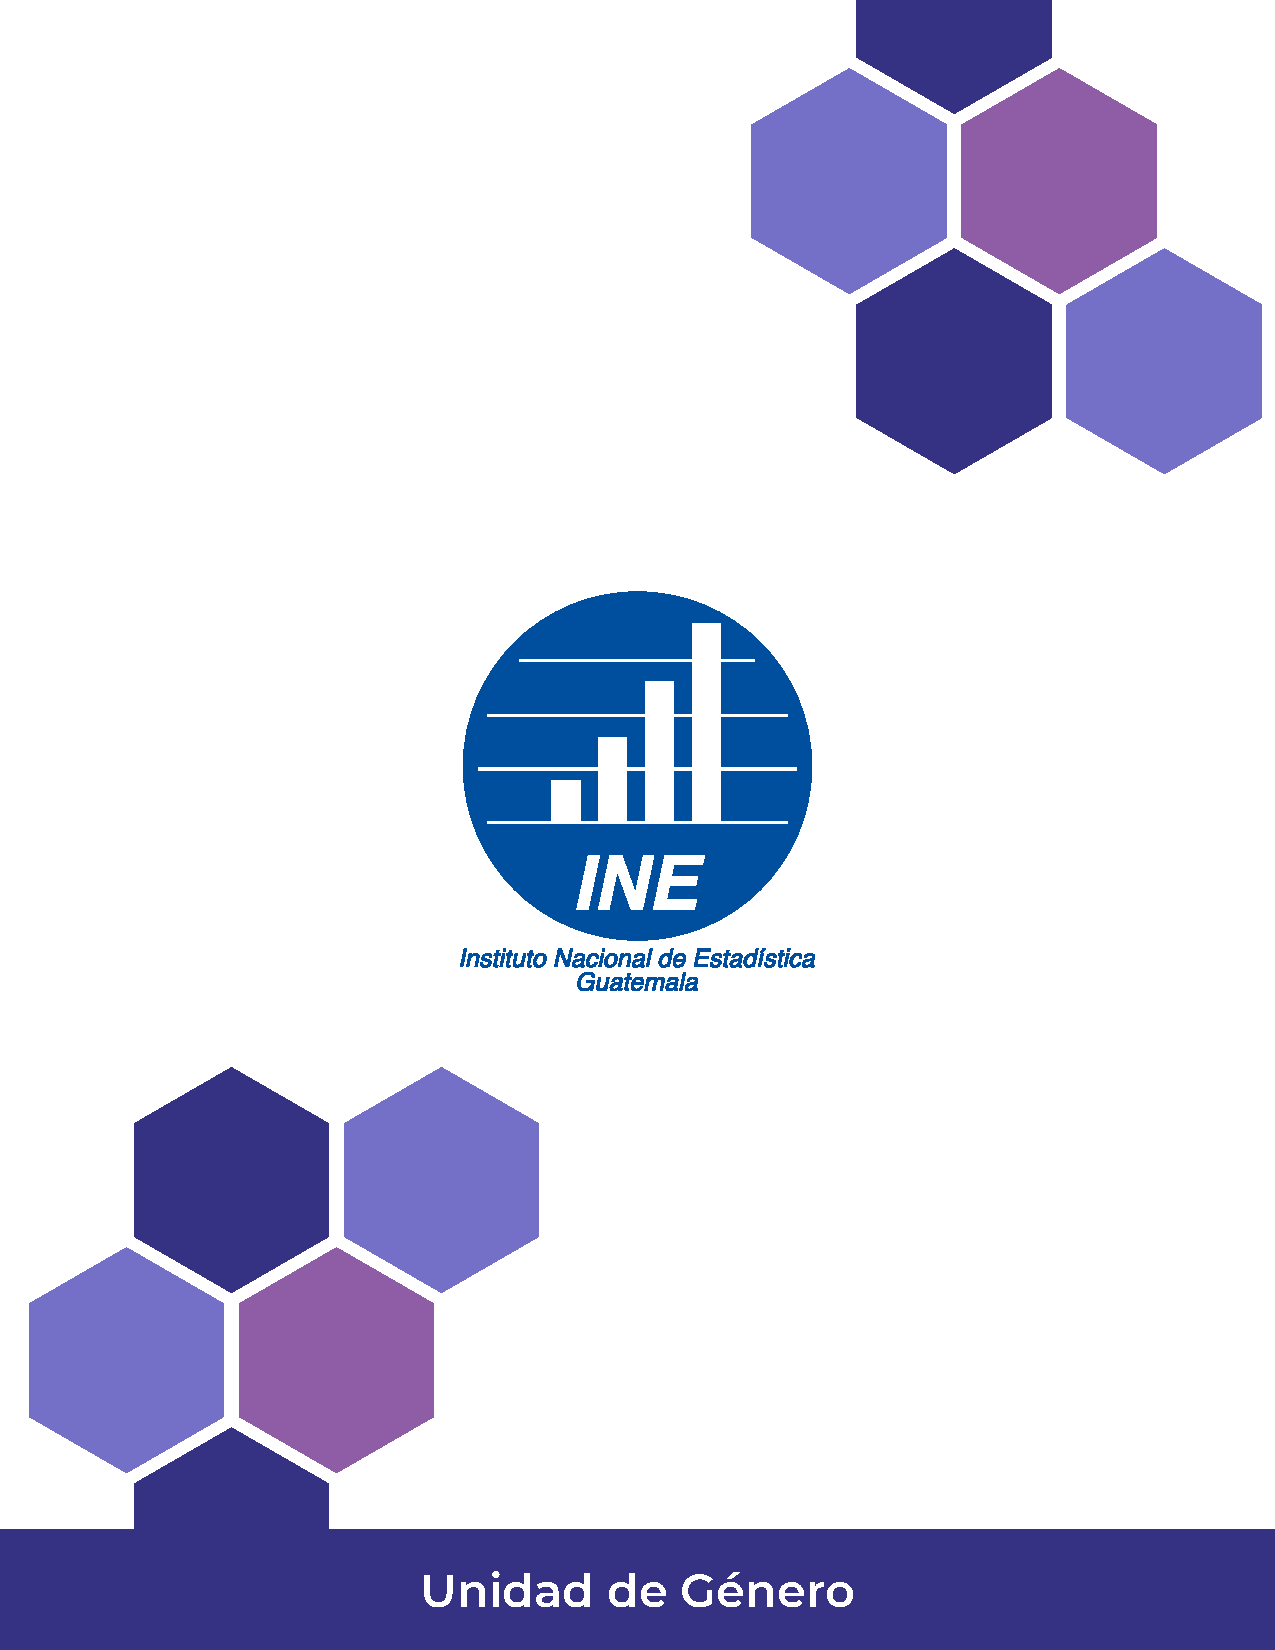
\includepdf{Plantilla/Contraportada_CEEG_2022.pdf}
	
	
\end{document}